% Copyright (C) 2007 Technical University of Liberec.  All rights reserved.
%
% Please make a following reference to Flow123d on your project site if you use the program for any purpose,
% especially for academic research:
% Flow123d, Research Centre: Advanced Remedial Technologies, Technical University of Liberec, Czech Republic
%
% This program is free software; you can redistribute it and/or modify it under the terms
% of the GNU General Public License version 3 as published by the Free Software Foundation.
%
% This program is distributed in the hope that it will be useful, but WITHOUT ANY WARRANTY;
% without even the implied warranty of MERCHANTABILITY or FITNESS FOR A PARTICULAR PURPOSE.
% See the GNU General Public License for more details.
%
% You should have received a copy of the GNU General Public License along with this program; if not,
% write to the Free Software Foundation, Inc., 59 Temple Place - Suite 330, Boston, MA 021110-1307, USA.
%
%%%%%%%%%%%%%%%%%%%%%%%%%%%%%%%%%%%%%%%%%%%%%%%%%%%%%%%%%%%%%%%%%%
%
% use PDFLatex to compile this
%

\documentclass[12pt,a4paper]{report}


\usepackage[utf8]{inputenc}
\usepackage{rotating}
\usepackage{pdflscape}
\usepackage{amssymb}
\usepackage{amsmath}
\usepackage{array}
\usepackage{longtable}
\usepackage[usenames,dvipsnames]{color}   %colors
\usepackage{colortbl}   %colorful tables
\usepackage{tabularx}
\usepackage{booktabs}
\usepackage{graphicx} %[dvips]
% it is note used \usepackage{cooltooltips}

%these two can be found in caption package
\usepackage{caption}
\usepackage{subcaption}

\usepackage[numbers]{natbib}

\usepackage{fancyvrb}   % extended verbatim environments (for examples of IO files)

\usepackage{multicol}
\usepackage{packages/multirow}
\usepackage{imakeidx}

% our own flow_doc.sty
% use hyperref package that must come after the imakeidx
\usepackage{flow_doc}


\renewcommand{\_}{\texttt{\symbol{'137}}}
\newcommand{\vari}[1]{{\it #1}}
\newcommand{\ditem}[2]{\item[\vari{#1} {\tt #2}]}
\newenvironment{fileformat}{\tt\begin{flushleft}}{\end{flushleft}}
%
%% ini table environment
\newcommand{\key}[1]{{\tt #1 }}
\newcommand{\type}[1]{{\bf #1}}
%
\newenvironment{initable}[1]{%
        \vspace{4ex}
        \noindent
        Section: \textbf{[#1]}\\
        \begingroup
        %%
        %% internal commands of initable environment
        %%
       \newcommand{\br}{\hfill\break}
        %%
        \renewcommand{\arraystretch}{1.4}
        \renewcommand{\tabcolsep}{2mm}
        \small
        \baselineskip 3ex
        %\begin{longtable}{@{}lp{5cm}p{5cm}p{9cm}}%
        \tabularx{\textwidth}{l>{\centering}p{2cm}>{\raggedright}p{2cm}>{\raggedright\arraybackslash}X}%
        %\renewcommand{\\}{\\[3ex]}%
        \hline\hline
        KEY & TYPE & DEFAULT & DESCRIPTION \\%\endhead
        \hline\hline
}{%
        %\end{longtable}
        \endtabularx
        \endgroup
}

%%%%%%%%%%%%%%%%%%%% specific math macros
\def\prtl{\partial}
\def\vc#1{\mathbf{\boldsymbol{#1}}}     % vector
\def\tn#1{{\mathbb{#1}}}    % tensor
\def\abs#1{\lvert#1\rvert}
\def\Abs#1{\bigl\lvert#1\bigr\rvert}
\def\div{{\rm div}}
\def\Lapl{\Delta}
\def\grad{\nabla}
\def\Real{{\mathbf R}}
\def\d {\,{\rm d}}
%% ini_table members


%paths to images
\def\fig{figures}
\def\test_fig{test_graphics}

\newcommand{\note}[1]{{\textbf{Note:} \textit{#1}}}
\newcommand{\tbd}[1]{{\textcolor{green}{TBD: #1}}}

%%%%%%%%%%%%%%%%%%%%%%%%%%%%%%%%%%%%%%%%%%%%%%%%%%%%%%%%%%%%%%%%%%%%%%%%%%%%%%%%%%%%%%%%%%%%% BEGIN DOCUMENT
%% set specific page layout
\addtolength{\textwidth}{2cm}
\addtolength{\hoffset}{-1.5cm}
\addtolength{\textheight}{4cm}
\addtolength{\voffset}{-2.5cm}

\makeindex[title=Alphabetical Index of Types]

\begin{document}

%%% remove comment delimiter ('%') and select language if required
%\selectlanguage{spanish} 
\thispagestyle{empty}
\begin{center}
\noindent 
\textbf{\LARGE{
  Technical university of Liberec
}}

\vspace{2ex}
\textbf{\LARGE{
  Faculty of mechatronics, informatics\\
  and interdisciplinary studies
}}

\vspace{160pt}

\textbf{\Huge{
Flow123d
}}

\vspace{1cm}
\textbf{\Large{
\input{flow_version}
}}

\vspace{1cm}

\textbf{\Large{
User Guide and Input Reference
}}

\vspace{9cm}




\noindent \textbf{\Large{Liberec, \the\year}}

\vspace{1cm}
\pagebreak
\end{center}

\noindent
{\bf Authors:}

\vspace{3ex}    
\noindent
Jan B\v rezina, Jan Stebel, David Flanderka, Pavel Exner

\vspace{3cm}
\noindent
{\bf Acknowledgment}

\vspace{3ex}
\noindent Release 3.9.0 was supported by the TA\v CR project no. TH03010227: Software pro komplexní a stochastické hydrogeologické modely.


% \noindent This work was supported by S\'URAO within the project Decovalex 2015, SO2013-077 and by the TA\v CR project no. TA04020506: 
% "Softwarov\'e n\'astroje pro simulaci a~anal\'yzu proces\r u v geosf\'e\v re".
\noindent 
\pagebreak
\noindent

\tableofcontents
\pagebreak
%\setcounter{page}{2}

\parindent=0pt
\parskip=1ex


\chapter{Getting Started}
\label{chapter:getting_started}

% Copyright (C) 2007 Technical University of Liberec.  All rights reserved.
%
% Please make a following reference to Flow123d on your project site if you use the program for any purpose,
% especially for academic research:
% Flow123d, Research Centre: Advanced Remedial Technologies, Technical University of Liberec, Czech Republic
%
% This program is free software; you can redistribute it and/or modify it under the terms
% of the GNU General Public License version 3 as published by the Free Software Foundation.
%
% This program is distributed in the hope that it will be useful, but WITHOUT ANY WARRANTY;
% without even the implied warranty of MERCHANTABILITY or FITNESS FOR A PARTICULAR PURPOSE.
% See the GNU General Public License for more details.
%
% You should have received a copy of the GNU General Public License along with this program; if not,
% write to the Free Software Foundation, Inc., 59 Temple Place - Suite 330, Boston, MA 021110-1307, USA.
%


\section{Introduction}
Flow123d is a~software for simulating water flow, reactionary solute transport, heat transfer, and mechanics in a~heterogeneous
porous and fractured medium. In particular, it is well-suited for simulations of underground processes in a~granite rock.
The program is able to describe explicitly processes in 3D medium, 2D fractures, and 1D channels and exchange between 
domains of different dimensions. Therefore, the computational mesh is a~collection of tetrahedra, triangles, and line segments.

Two water flow models are available: a model for a~saturated medium based on the Darcy law
and a~model for a~partially saturated medium described by Richards' equation.
Both models use the mixed-hybrid finite element method for the space discretization and the implicit Euler method for the time discretization.
Both models can also switch between a~transient case and a~sequence of steady states within a~single simulation. The model for unsaturated medium uses
a lumped variant of the mixed-hybrid method to satisfy the maximum principle and to guarantee stability for short time steps.

In the current version,  only the model for saturated media can be sequentially coupled  with the transport models, including
two models for the solute transport and one model for the heat transfer.

The first solute transport model can deal only with a~pure advection of several substances without any diffusion-dispersion term. It uses
the explicit Euler method for the time discretization and the finite volume method for the space discretization.
The second solute transport model describes a~general advection with hydrodynamic dispersion for several substances.
It uses the implicit Euler method for time discretization and the discontinuous Galerkin method of
the first, second, or third order for the discretization in space.
The operator splitting method can be used to couple any of these two solute transport models with  
 various processes described by the reaction term. The reaction term can treat any meaningful combination of the dual porosity,
equilibrium sorptions, decays, and linear reactions.

The heat transfer model assumes equilibrium between the temperature of the rock and of the fluid phase. It uses the same numerical scheme as the second transport model, i.e., the DG method with the implicit time discretization.

The mechanical model computes linear elastic problems, taking into account the reduced dimension approach.
It can be coupled with the flow model and solve linear poroelastic problems. This coupling is realized by an iterative scheme. Nonlinear dependency between strain and hydraulic conductivity and nonlinearity due to contacts and shear stress effects is the focus of ongoing development.

The program supports the output of all input and output fields into two file formats. One can use the GMSH mesh generator and post-processor file format or the output into widely supported VTK format. In particular, we recommend Paraview software for the visualization and post-processing of the VTK data.

The program is implemented in C/C++ using the PETSc library for linear algebra. All models can run in parallel using the MPI environment; however, the scalability of the whole program is limited due to serial mesh data structures and serial outputs.


The program is distributed under GNU GPL v. 3 license and is available on the project web page:
\url{http://flow123d.github.io}

with sources on the GitHub:
\url{https://github.com/flow123d/flow123d}.


\section{Reading Documentation}
The Flow123d documentation has two main parts. Chapters \ref{chapter:getting_started} to \ref{chapter:tutorials} form a user
manual, while the last Chapter \ref{chapter:input-tree-reference} provides an input reference.
The user manual starts with Chapter \ref{chapter:getting_started} giving instructions for the installation and execution of the program.
The Chapter \ref{chapter:mathematical_models} provides a detailed description of the implemented mathematical models. The
Chapter \ref{chapter:numerical} presents used numerical methods.
The input and output file formats are documented in Chapter \ref{chapter:file-formats}.
Finally, Chapter \ref{chapter:tutorials} consists of tutorial problems.

The input reference guide, consisting only of Chapter \ref{chapter:input-tree-reference}, is automatically generated.
It mirrors the code directly and describes the whole structure of the main input file. Description
of input records, their structure, and default values are supplied there, and bidirectional links to the user manual are provided.

The document is interactive; the {\color{blue}blue text} marks the links in the document, and the {\color{magenta}magenta text} marks the web links.




\section{Installing Flow123d}
Software Flow123d requires the tool \href{https://www.docker.com}{Docker}. Docker is an open-source project that automates
the deployment of Linux applications inside software containers. Entire Flow123d software is packed in a~Docker image that
also contains necessary libraries and crucial components of the Linux operating system.

The installation process imports the Docker image into the user's machine and personalizes the Docker image.
The installation instructions for Linux and Windows operating systems are provided in the two following sections.


\subsection{Installing Flow123d on Linux}
The installation is done under a~regular user, who must be in the group 'docker'.
Download the Linux installation package archive
\begin{center}
\verb'flow123d_<version>_linux_install.tar.gz'
\end{center}
from \href{http://flow123d.github.io/}{Official pages} and extract it to any folder:
\begin{verbatim}
  $> tar -xzf flow123d_<version>_linux_install.tar.gz
\end{verbatim}
This will create a~directory \verb'flow123d_<version>'. In the next step, navigate to this directory
and execute the \verb'install.sh' script. Example output:
\begin{verbatim}
  $> cd flow123d_3.0.4
  $> ./install.sh
  Pulling docker image 'flow123d/3.0.4'
  ...
  flow123d/3.0.4
  Installation of Flow123d finished successfully.
  Run Flow123d using script fterm.sh or flow123d.sh in bin folder.
  You can start by printing the version of Flow123d:
    bin/fterm.sh run --version
\end{verbatim}
The install script will download Docker image from the \href{https://hub.docker.com/u/flow123d}{Docker Hub}.
% The script will also print additional information during personalization process.
Whole process may take several minutes (depending on user's machine performance and internet connectivity).


% \subsubsection{Alternate way to install}
% Assuming having \href{https://www.docker.com}{Docker} installed, one can simply run:
% \begin{verbatim}
%   > curl -s https://flow.nti.tul.cz/get | bash
% \end{verbatim}
% This will check user's system and download scripts \verb'flow123d' and \verb'fterm'.
% Then the user can continue by running 
% \begin{verbatim}
%   > fterm --version 3.0.4 run
% \end{verbatim}
% to open the shell of the Docker container. This will download the Docker image of the selected version
% if it is not already available.

\subsection{Installing Flow123d on Windows}
\subsubsection{Before you install}

This version uses \verb'Docker for Windows', previous versions which used \verb'Docker Toolbox' will \textbf{stop working}.

Make sure your system fullfills following requirements in order to support \verb'Docker for Windows':
\begin{itemize}
    \item Windows 10 64bit: Pro, Enterprise or Education (1607 Anniversary Update, Build 14393 or later).
    \item Virtualization is enabled in BIOS. Typically, virtualization is enabled by default. This is different from having Hyper-V enabled. For more detail see \href{https://docs.docker.com/docker-for-windows/troubleshoot/#virtualization-must-be-enabled}{Virtualization must be enabled} in Troubleshooting.
    \item CPU SLAT-capable feature.
    \item At least 4GB of RAM.
\end{itemize}


\subsubsection{Installation}

To install Flow123d on Windows, download installer from \href{http://flow123d.github.io/}{Official pages}, execute it and follow instructions
on your screen. To make things easier, you can also \href{https://www.youtube.com/watch?v=xDR2vU-1IhM}{watch a installation video}.

If for some reason the installation failed, make sure eveything below is in order:


\subsubsection{Flow123d troubleshooting}

\begin{itemize}
  \item \textbf{Powershell is installed}: On the Windows systems we require PowerShell. Windows PowerShell needs to be installed on Windows Server 2008 and Windows Vista only.
  It is already installed on Windows Server 2008 R2 and Windows 7 and higher. To install PowerShell follow instructions at
  \href{https://msdn.microsoft.com/en-us/powershell/scripting/setup/installing-windows-powershell}{Microsoft pages}.

  \item \textbf{Powershell is in the system PATH}: Make sure \verb'powershell' command is in the system PATH.
  \href{http://www.powershelladmin.com/wiki/PowerShell_Executables_File_System_Locations}{PowerShell executable location}
   is specific to the particular Windows version, but usual location is:
   \begin{verbatim}
      %SystemRoot%\system32\WindowsPowerShell\v1.0\powershell.exe
   \end{verbatim}
   To add this location to the system PATH variable follow the instructions at
   \href{https://msdn.microsoft.com/en-us/library/office/ee537574(v=office.14).aspx}{Microsoft pages}.

   \item For detailed instructions refer to \href{https://docs.docker.com/docker-for-windows/}{Docker docs}.
\end{itemize}


\subsubsection{Uninstalling Flow123d}
To uninstall Flow123d, in Windows open \verb'Apps & features' (\verb'Aplikace a funkce' in Czech), find the Flow123d in the list
and click uninstall. This will only uninstall the Flow123d but not \verb'Docker for Windows'.


\subsubsection{Reinstalling Flow123d}
\label{duplicit-image}
If you are installing same version of Flow123d again, installation process will be the same,
except \verb'Docker for Windows' installation will be skipped.


\section{Running Flow123d}
\subsection{Running Flow123d on Linux}
\label{subsec:running-flow123d-on-linux}
All necessary scripts for running Flow123d are located in the \verb'bin' subdirectory of the installation directory \verb'flow123d_<version>'.
From the user's perspective, an unpleasant issue with the Docker container is that it cannot easily interact with the host file system by default.
Using the supplied scripts in \verb'bin' will make things a~lot easier for the user.
The directory \verb'bin' contains:
\begin{itemize}
	\item \verb'fterm.sh' \\
	 The script will invoke a~shell inside the Docker container and mount the user's home directory.
	 In this shell, the user has access to the system path where Flow123d is installed.
	 By default, the command \verb'flow123d' is in the \verb'PATH' variable.
	 
	\note{ On some systems, the shell's font is extremely small, you can change this behavior by right-clicking on the window bar and selecting} 
	\verb'default' \emph{or} (\verb'vychozi' in Czech) \emph{see \autoref{fig:TerminalFont}.}
	 \begin{figure}
		 \center
		 \includegraphics[width=1\textwidth]{\fig/TerminalFont.png}
		 \caption{Changing default font family and font size}
		 \label{fig:TerminalFont}
	 \end{figure}

	\item \verb'flow123d.sh' \\
	 The script will run Flow123d inside the Docker container and mount the user's home directory.
	 All arguments passed to this script will be passed to \verb'flow123d' binary file inside the container.

	\item \verb'runtest.sh' \\
	 The script will run Flow123d tests inside the Docker container and mount the user's home directory.
	 All arguments passed to this script will be passed to \verb'runtest.py' Python script inside the container.
\end{itemize}

\note{ Using the above} \verb'.sh'
\emph{scripts will mount the user's home directory to the Docker container under the same name.
Also your current working directory will be the same. The example below shows the behavior of the scripts:}
\begin{verbatim}
$> pwd
/home/username/local/flow123d_3.0.4

$> ls
bin  doc  install.sh  tests uninstall.sh

$> bin/fterm.sh
 ___ _            _ ___ ____   _
| __| |_____ __ _/ |_  )__ / __| |
| _|| / _ \ V  V / |/ / |_ \/ _  |
|_| |_\___/\_/\_/|_/___|___/\__,_|
                         3.0.4
flow@flow:3.0.4 /home/username/local/flow123d_3.0.4$> ls
bin  doc  install.sh  tests uninstall.sh
\end{verbatim}


\subsection{Running Flow123d on Windows}
On system Windows you will have a shortcut on your desktop, to verify everything is working. To run flow123d from anywhere simple type
\verb'flow123d.bat' or \verb'fterm.bat' (in terminal, powershell, Total Commander, \dots).

Each bat file serves a different purpose:
\begin{itemize}
  \item \verb'flow123d.bat' serves as a binary, it possible to run the bat file multiple times (useful for a batch processing)
  \item \verb'fterm.bat' serves as an interactive shell console session invoked inside Docker container.
\end{itemize}

By default \verb'flow123d.bat' will run the last installed version on your system. If you have multiple version installed and want to run specific one, each version has a unique bat files \verb'flow123d-<version>.bat' and \verb'fterm-<version>.bat' file (e.g. \verb'flow123d-3.0.9.bat' and \verb'fterm-3.0.9.bat').


\subsubsection{Running from other batch file}
The Windows system calls the batch files in the different way then the binaries. In particular the calling batch file is not processed further after the child batch
file is done. In order to do so, one have to use the \verb'CALL' command. This is especially necessary for various calibration tools. The correct calling batch file
may look like:
\begin{verbatim}
    echo "Starting Flow123d ..."
    call flow123d.bat a_simulation.yaml
    echo "... simulation done."
\end{verbatim}


\subsubsection{Adjusting memory of virtual machine}
To change the memory limits of the Virtual machine, open the Docker Settings dialog (right click on the whale icon) and select \verb'Settings'.
Navigate to \verb'Advanced' tab and adjust the memory. Detailed instructions can be found \href{https://docs.docker.com/docker-for-windows/#advanced}{Docker docs}.


\section{Flow123d arguments}
When you are inside of the Docker container, you have access to the entire file system of the container. Flow123d is installed in \verb'/opt/flow123d' directory. Folder \verb'bin' contains binary files and is automatically
added to the variable \verb'PATH', so that every executable in this folder can be called from anywhere.

The main Flow123d binary is located in \verb'bin/flow123d' and accepts the following arguments:
\begin{description}
 \item[{\tt --help}] \hfill\\
        Help for parameters interpreted by Flow123d. Remaining parameters are passed to PETSC.
 \item[ {\tt -s, --solve} ] \verb'<file>' \hfill\\
 	 Set principal input file. Can be in YAML (or  JSON) file format. All relative paths of the input
 	 files are relative to the location of the principal input file.
 \item[{\tt -i, --input\_dir}] \verb'<directory>' \hfill\\
 	The placeholder \verb"${INPUT}" %$
  	used in the path of an input file will be replaced by the \verb'<directory>'. Default value is \verb'input'.
 \item[{\tt -o, --output\_dir}] \verb'<directory>' \hfill\\
 	All paths for output files will be relative to this \verb'<directory>'. Default value is \verb'output'.
 \item[{\tt -l, --log}] \verb'<file_name>' \hfill\\
 	Set base name of log files. Default value is \verb'flow123d'. The log files are individual for every MPI process, placed in the output directory.
 	The MPI rank of the process and the \verb'log' suffix are appended to the base name.
 \item[{\tt --version}] \hfill\\
        Display version and build information.
 \item[{\tt --no\_log}] \hfill\\
        Turn off logging.
 \item[{\tt --no\_profiler}] \hfill\\
        Turn off profiler output.
 \item[{\tt --petsc\_redirect <file>}] \hfill\\
        Redirect all PETSc stdout and stderr to given file.
 \item[{\tt --input\_format}] \hfill\\
        Print a~description of the main input file in JSON format.
        This is used by GeoMop model editor and by python scripts for
        generating reference documentation in Latex or HTML format.
 \item[{\tt --yaml\_balance}] \hfill\\
        Generate balance file also in machine readable YAML format. Will be default in future, used by GeoMop.
 \item[{\tt --no\_signal\_handler}] \hfill\\
        For debugging purpose.
\end{description}

The {\tt -s} identifier can be skipped:
\begin{verbatim}
  flow123d <main_input>.yaml <options> <PETSC options>
\end{verbatim}

Any different parameters are passed to the PETSC library. An advanced user can influence lot of parameters of linear solvers. In order to get list of supported options
use parameter \verb'-help' together with a~valid input file. Options for various PETSC modules are displayed when the module is used for the first time.

Alternatively, you can use python script \verb'exec_parallel' located in \verb'bin/python' to start parallel jobs or limit resources used by the program.

After double dash specify which \verb'mpiexec' binary will be used (\verb'MPI-EXECUTABLE') and then specify what should be executed.
The script does not need to run solely \verb'flow123d'.

If we want to run command \verb'whoami' in parallel we can do:
\begin{verbatim}
	bin $> exec_parallel -n 4 -- ./mpiexec whoami
\end{verbatim}

To execute Flow123d in parallel we can do:
\begin{verbatim}
	bin $> exec_parallel -n 4 -- ./mpiexec ./flow123d --help
\end{verbatim}


\begin{verbatim}
  exec_parallel [OPTIONS] -- [MPI-EXECUTABLE] [PARAMS]
\end{verbatim}

The script has following options:

\begin{description}
  \item[{\tt -h, --help}] \hfill\\
  	Usage overview.
  \item[{\tt --host}] \verb'<hostname>' \hfill\\
  		Valid only when option \verb'--queue' is set.
        Default value is the host name obtained by python \verb'platform.node()' call, this argument can be used to override it.
        Resulting value is used to select a~correct PBS module from lookup table \verb'config/host_table.yaml'.
  \item[{\tt -n}] \verb'<number of processes>' \hfill\\
  	Specify number of MPI parallel processes for calculation.
  \item[{\tt -t, --limit-time}] \verb'<timeout>' \hfill\\
  	Upper estimate for real running time of the calculation. Kill calculation after {\it timeout} seconds.
  	Value can also be \verb'float' number. When in PBS mode, value can also affect PBS queue.
  \item[{\tt -m, --limit-memory}] \verb'<memory limit>' \hfill\\
  	Limits total available memory to \verb'<memory limit>' MB in total.
  \item[{\tt -q, --queue}] \verb'<queue>' \hfill\\
  		If set activates PBS mode. If argument \verb'queue' is also set selects particular job queue
  		on PBS systems otherwise default PBS queue is used. Default PBS queue automatically
  		choose valid queue based on resources.
\end{description}


Another script which runs Flow123d is \verb'runtest.sh'. This script will run tests specified as arguments. Script accepts both folders
and yaml files. To see full details run \verb'runtest.sh --help'. The script will run yaml tests and then compare results with reference
output. Example usage of the script:

\begin{verbatim}
$> bin/runtest.sh tests/10_darcy/01_source.yaml
configuration:
------------------------------------------------------------
  yaml files       1
  total cases      2
------------------------------------------------------------
execution:
  done [01 of 02] 1 x 10_darcy/01_source [00:03.070] [31 MiB] exitcode 0
  done [02 of 02] 2 x 10_darcy/01_source [00:01.378] [31 MiB] exitcode 0
------------------------------------------------------------
SUMMARY 
------------------------------------------------------------
  [ PASSED ]  | 1 x 10_darcy/01_source                        [ 2.76 sec] 
  [ PASSED ]  | 2 x 10_darcy/01_source                        [ 1.07 sec] 
  ------------------------------------------------------------
  [ PASSED ]  | passed=2, failed=0, skipped=0 in              [ 3.83 sec]
------------------------------------------------------------
\end{verbatim}




\section{Tutorial Problem}
In the following section, we shall provide an example cookbook for preparing and running a~model
based on one of the test problems, namely
\begin{verbatim}
    tests/21_solute_fv_frac/03_fv_dp_sorp_small.yaml.
\end{verbatim}
We shall start with the preparation of the geometry using external software, and then we shall go step by step through the
commented main input file. The problem includes steady Darcy flow, transport of two substances with explicit
time discretization, and a~reaction term consisting of dual porosity and sorption models.
More tutorials focused on particular features can be found in Chapter \ref{chapter:tutorials}.

\subsection{Geometry}
We consider a~simple 2D problem with a~branching 1D fracture (see Figure \ref{fig:tutorial} for the geometry). 
To prepare a~mesh file we use the \href{http://geuz.org/gmsh/}{GMSH software}.
First, we construct a~geometry file. In our case the geometry consists of: 
\begin{itemize}
 \item one physical 2D domain corresponding to the whole square
 \item three 1D physical domains of the fracture
 \item four 1D boundary physical domains of the 2D domain
 \item three 0D boundary physical domains of the 1D domain
\end{itemize}
In this simple example, we can in fact combine physical domains in every group, however we use this more complex setting for
demonstration purposes. Using GMSH graphical interface we can prepare the GEO file where physical domains are referenced by numbers, then we use 
any text editor and replace numbers with string labels in such a~way that the labels of boundary physical domains start with the dot character. 
These are the domains where we will not do any calculations but we will use them for setting boundary conditions.
Finally, we get the GEO file like this:

\begin{multicols}{2}
{\small
\begin{Verbatim}[numbers=left]
cl1 = 0.16;
Point(1) = {0, 1, 0, cl1};
Point(2) = {1, 1, 0, cl1};
Point(3) = {1, 0, 0, cl1};
Point(4) = {0, 0, 0, cl1};
Point(6) = {0.25, -0, 0, cl1};
Point(7) = {0, 0.25, 0, cl1};
Point(8) = {0.5, 0.5, -0, cl1};
Point(9) = {0.75, 1, 0, cl1};
Line(19) = {9, 8};
Line(20) = {7, 8};
Line(21) = {8, 6};
Line(22) = {2, 3};
Line(23) = {2, 9};
Line(24) = {9, 1};
Line(25) = {1, 7};
Line(26) = {7, 4};
Line(27) = {4, 6};
Line(28) = {6, 3};
\end{Verbatim}
\columnbreak
\begin{Verbatim}[numbers=left, firstnumber=last]
Line Loop(30) = {20, -19, 24, 25};
Plane Surface(30) = {30};
Line Loop(32) = {23, 19, 21, 28, -22};
Plane Surface(32) = {32};
Line Loop(34) = {26, 27, -21, -20};
Plane Surface(34) = {34};
Physical Point(".1d_top") = {9};
Physical Point(".1d_left") = {7};
Physical Point(".1d_bottom") = {6};
Physical Line("1d_upper") = {19};
Physical Line("1d_lower") = {21};
Physical Line("1d_left_branch") = {20};
Physical Line(".2d_top") = {23, 24};
Physical Line(".2d_right") = {22};
Physical Line(".2d_bottom") = {27, 28};
Physical Line(".2d_left") = {25, 26};
Physical Surface("2d") = {30, 32, 34};
\end{Verbatim}
}
\end{multicols}

Notice the labeled physical domains on lines 26 -- 36. Then we just set the discretization step \verb'cl1' and use GMSH to create the mesh file.
The mesh file contains both the 'bulk' elements where we perform calculations and the 'boundary' elements (on the boundary physical domains) where we only set the boundary conditions.

\subsection{YAML File Format}
The main input file uses the YAML file format with some restrictions. 
We prefer to call YAML objects \emph{records} and we introduce also \emph{abstract records}
that mimic C++ abstract classes.
Arrays have only elements of the same type (possibly using abstract record types for polymorphism). 
The usual keys are in lower case and without spaces (using underscores instead).
For detailed description see Section \ref{sec:CONformat}.


Having the computational mesh from the previous step, we can create the main input file with the description of our problem. 
\begin{Verbatim}[numbers=left]
flow123d_version: 3.1.0
problem: !Coupling_Sequential
  description: 'Transport 1D-2D (convection, reaction term, sources).'
  mesh:
    mesh_file: ../00_mesh/square_1x1_frac_fork.msh
    regions:
      - !Union
        name: 1d_domain
        regions:
          - 1d_upper
          - 1d_lower
          - 1d_left_branch
\end{Verbatim}
The version of Flow123d for which the file is a~valid input is specified at the first line.
Then the description starts with a~selection of the problem type (\verb'Coupling_Sequential'), and a~textual problem description.
Next, the computational mesh is defined; here it consists of the name of the mesh file and the declaration of one region
given as the union of all 1D regions, i.e., representing the whole fracture. Other keys of the \Alink{IT::Mesh}{\tt mesh} record allow labeling regions given only by numbers,
defining new regions in terms of element numbers (e.g to have a~leakage on single element),
defining boundary regions, and several operations with region sets, see Section \ref{sec:Mesh} for details.

\subsection{Flow Setting}
Next, we setup the flow problem. We shall consider a~steady flow (i.e. with zero storativity) driven only by the pressure gradient (no gravity),
setting the Dirichlet boundary condition on the whole boundary with the pressure head equal to $x+y$. 
The \Alink{Flow-Darcy-MH-Data::conductivity}{\tt conductivity} will be $k_2=10^{-7}$ \unitss{}{1}{-1} on the 2D domain and $k_1=10^{-6}$ \unitss{}{1}{-1} on the 1D domain.
We leave the default value for the \Alink{Flow-Darcy-MH-Data::cross-section}{\tt cross\_section} of the 2D domain,
meaning that the thickness of 2D domain is $\delta_2=1$ \unitss{}{1}{}.
For the 1D fractures cross-section, we prescribe $\delta_1=0.04$ \unitss{}{2}{} on the 1D domain.
The transition coefficient $\sigma_2$ between dimensions can be scaled by setting the dimensionless parameter 
$\sigma_{21}$ (\Alink{Flow-Darcy-MH-Data::sigma}{\tt sigma}). This can be used for simulating additional
effects which prevent the liquid transition from/to a~fracture, like a~thin resistance layer.
Notice that the scaling parameter is set on the lower dimensional domain, i.e. $\sigma_{21}=0.9$ on line \ref{vrb:tutorial_flow_input_sigma}.
Read Section \ref{sec:darcy_flow} for more details.

\begin{Verbatim}[numbers=left, firstnumber=last,commandchars=\\\{\}]
  flow_equation: !Flow_Darcy_MH\label{vrb:tutorial_floweq}
    input_fields:\label{vrb:tutorial_flow_input_start}
      - region: 1d_domain
        conductivity: 1.0e-06
        cross_section: 0.04
        sigma: 0.9\label{vrb:tutorial_flow_input_sigma}
      - region: 2d
        conductivity: 1.0e-07
      - region: .BOUNDARY
        bc_type: dirichlet
        bc_pressure: !FieldFormula
          value: x+y\label{vrb:tutorial_flow_input_end}
    nonlinear_solver:
      linear_solver: !Petsc
        a_tol: 1.0e-12
        r_tol: 1.0e-12
    output:\label{vrb:tutorial_output_start}
      fields:
        - pressure_p0
        - velocity_p0\label{vrb:tutorial_output_end}
    output_stream:
      file: flow.pvd
      format: !vtk
        variant: ascii
\end{Verbatim}
% Tutorial also has output of pressure_p1 is it still supported?
%
On line \ref{vrb:tutorial_floweq}, we specify particular implementation (numerical method) of the flow solver, in this case the Mixed-Hybrid
solver for steady problems. On lines \ref{vrb:tutorial_flow_input_start} -- \ref{vrb:tutorial_flow_input_end} in the array \hyperA{IT::Flow-Darcy-MH-Data}{\tt input\_fields}, 
we set both mathematical fields that live on the computational domain 
and those defining the boundary conditions.
We use implicitly defined region \verb'.BOUNDARY' that contains all boundary regions and we set there Dirichlet boundary condition in terms of the
pressure head. In this case, the field is not of the implicit type {\tt FieldConstant}, so we must specify the type of the field {\tt !FieldFormula}.
See Section \ref{sec:Fields} for other field types. 
Next, we specify the type of the linear solver and its tolerances.
On lines \ref{vrb:tutorial_output_start} -- \ref{vrb:tutorial_output_end}, we specify which output fields should be written to the output stream
(that means particular output file, with given format). See Section \ref{section_output} for the list of available output \Alink{IT::Flow-Darcy-MH-OutputFields}{\tt fields}.
Currently, we support only one \Alink{IT::OutputStream}{\tt output\_stream} per equation. We specify the filename and the format of the output stream (the used ASCII VTK format is the default).



\subsection{Transport Setting}
The flow model is followed by a~transport model in the record \Alink{Coupling-Sequential::solute-equation}{\tt solute\_equation}
beginning on line \ref{vrb:tutorial_solute_start}. Here, we use an implementation called \hyperA{IT::Solute-Advection-FV}{Solute\_Advection\_FV}
which stands for an explicit finite volume solver of the convection equation (without diffusion).
The operator splitting method is used for equilibrium sorption as well as for dual porosity model and 
first order reactions simulation.

\begin{Verbatim}[numbers=left, firstnumber=last,commandchars=\\\{\}]
  solute_equation: !Coupling_OperatorSplitting\label{vrb:tutorial_solute_start}
    substances:\label{vrb:tutorial_substances_start}
      - name: age # water age
        molar_mass: 0.018
      - name: U235 # uranium 235
        molar_mass: 0.235\label{vrb:tutorial_substances_end}
    transport: !Solute_Advection_FV
      input_fields:\label{vrb:tutorial_transport_input_start}
        - region: ALL
          init_conc: 0\label{vrb:tutorial_transport_init_conc}
          porosity: 0.25
          # source is in the whole volume (l+s) -> times porosity
          sources_density:
            - 0.25
            - 0
        - region: .BOUNDARY\label{vrb:tutorial_transport_boundary}
          bc_conc:
            - 0.0
            - 1.0\label{vrb:tutorial_transport_input_end}
    time:
      end_time: 1000000
    balance:
      cumulative: true
\end{Verbatim}

On lines \ref{vrb:tutorial_substances_start} -- \ref{vrb:tutorial_substances_end}, we set the transported \Alink{Coupling-OperatorSplitting::substances}{\tt substances}, 
which are identified by their names. Here, the first one is the \verb'age' of the water, with the molar mass of water, 
and the second one \verb'U235' is the uranium isotope 235. 
On lines \ref{vrb:tutorial_transport_input_start} -- \ref{vrb:tutorial_transport_input_end}, we set the input fields, in particular zero initial concentration for all substances,
\Alink{Solute-Advection-FV-Data::porosity}{\tt porosity} $\theta = 0.25$ and 
sources of concentration by \Alink{Solute-Advection-FV-Data::sources-density}{\tt sources\_density}. 
Notice line \ref{vrb:tutorial_transport_init_conc} where we can see only single value since an automatic conversion is applied to turn the scalar 
zero into the zero vector (of size 2 according to the number of substances). 

The boundary fields are set on lines \ref{vrb:tutorial_transport_boundary} -- \ref{vrb:tutorial_transport_input_end}. We do not need to specify the type of the condition since there is 
only one type in the {\tt Solute\_Advection\_FV} transport model. The boundary condition is equal to $1$ for the uranium 235 and $0$ 
for the age of the water and is automatically applied only on the inflow part of the boundary. 

We also have to prescribe the \hyperA{IT::TimeGovernor}{\tt time} setting -- here it is only the end time of the simulation
(in seconds: $10^6\,\rm{s}\approx 11.57$ days). The step size is determined automatically from the CFL condition,
however, a~smaller time step can be enforced if necessary.

Reaction term of the transport model is described in the next subsection, including dual porosity and sorption.

\subsection{Reaction Term}\label{subsubsec:reactions}
The input information for dual porosity, equilibrial sorption and possibly first order reactions are enclosed in the record 
\Alink{Coupling-OperatorSplitting::reaction-term}{\tt reaction\_term}, lines \ref{vrb:tutorial_dp_start} -- \ref{vrb:tutorial_dp_end}. Go to section \ref{sec:reaction_term}
to see how the models can be chained.

The type of the first process is determined by {\tt !DualPorosity}, on line \ref{vrb:tutorial_dp_start}. 
The \Alink{DualPorosity::input-fields}{\tt input\_fields}
of the dual porosity model are set on lines \ref{vrb:tutorial_dp_input_start} -- \ref{vrb:tutorial_dp_input_end} and the output is disabled by setting an empty array on line \ref{vrb:tutorial_dp_output}.

\begin{Verbatim}[numbers=left, firstnumber=last,commandchars=\\\{\}]
    reaction_term: !DualPorosity\label{vrb:tutorial_dp_start}
      input_fields:\label{vrb:tutorial_dp_input_start}
        - region: ALL
          diffusion_rate_immobile:
            - 0.01
            - 0.01
          porosity_immobile: 0.25
          init_conc_immobile:
            - 0.0
            - 0.0\label{vrb:tutorial_dp_input_end}
      output:
        fields: []\label{vrb:tutorial_dp_output}
      reaction_mobile: !SorptionMobile\label{vrb:tutorial_sorp_mob}
        solvent_density: 1000.0 # water\label{vrb:tutorial_sorp_mob_param_start}
        substances:
          - age
          - U235
        solubility:
          - 1.0
          - 1.0\label{vrb:tutorial_sorp_mob_param_end}
        input_fields: &anchor1\label{vrb:tutorial_sorp_mob_input_start}
          - region: ALL
            rock_density: 2800.0 # granite
            sorption_type:
              - none
              - freundlich
            distribution_coefficient:
              - 0
              - 1.598e-4
            isotherm_other:
              - 0
              - 1.0\label{vrb:tutorial_sorp_mob_input_end}
        output:
          fields: []\label{vrb:tutorial_sorp_mob_output}
      reaction_immobile: !SorptionImmobile\label{vrb:tutorial_sorp_immob}
        solvent_density: 1000.0 # water
        substances:
          - age
          - U235
        solubility:
          - 1.0
          - 1.0
        input_fields: *anchor1\label{vrb:tutorial_sorp_immob_input}
        output:
          fields: []\label{vrb:tutorial_dp_end}
    output_stream:\label{vrb:tutorial_trans_output_start}
      file: transport.pvd
      format: !vtk
        variant: ascii
      times:
        - step: 100000.0\label{vrb:tutorial_trans_output_end}
\end{Verbatim}

Next, we define the equilibrial sorption model such that \hyperA{IT::SorptionMobile}{\tt SorptionMobile} type takes place in the mobile 
zone of the dual porosity model while \hyperA{IT::SorptionImmobile}{\tt SorptionImmobile} type takes place in its immobile zone, see lines \ref{vrb:tutorial_sorp_mob} and \ref{vrb:tutorial_sorp_immob}.
Isothermally described sorption simulation can be used in the case of low concentrated solutions without competition between multiple dissolved species.

On lines \ref{vrb:tutorial_sorp_mob_param_start} -- \ref{vrb:tutorial_sorp_mob_param_end}, we set the sorption related input information. The solvent is water so the \Alink{Sorption::solvent-density}{\tt solvent\_density} 
is supposed to be constant all over the simulated area. The vector \Alink{Sorption::substances}{\tt substances} 
contains the list of names of solute substances which are considered to be affected by the sorption.
Solubility is a~material characteristic of a~sorbing substance related to the solvent. Elements of the vector 
\Alink{Sorption::solubility}{\tt solubility} define the upper bound of aqueous concentration which can appear.
This constrain is necessary because some substances might have limited solubility and if the solubility exceeds 
its limit they start to precipitate. {\tt solubility} is a~crucial parameter for solving a~set of nonlinear 
equations, described further. 

The record \hyperA{IT::Sorption-Data}{\tt input\_fields} covers the region specific parameters.
All implemented types of sorption can take the rock density in the region into account. The value of 
\Alink{Sorption-Data::rock-density}{\tt rock\_density} is a~constant in our case. 
The \Alink{Sorption-Data::sorption-type}{\tt sorption\_type} represents the empirically determined isotherm 
type and can have one of four possible values: \{{\tt"none"}, {\tt"linear"}, {\tt"freundlich"}, {\tt"langmuir"}\}. 
Linear isotherm needs just one parameter given whereas Freundlich and Langmuir isotherms require two parameters. 
We will use Freundlich isotherm for demonstration but we will set the other parameter (exponent) $\alpha=1$ 
which means it will be the same as the linear type. We use value 
$K_d=1.598\cdot10^{-4}$ \unitss{-1}{3}{} for the 
\Alink{Sorption-Data::distribution-coefficient}{\tt distribution\_coefficient} 
according to (www.skb.se, report R-10-48 by James Crawford, 2010).
 

On line \ref{vrb:tutorial_sorp_immob_input}, notice the reference pointing to the definition of input fields on lines \ref{vrb:tutorial_sorp_mob_input_start} -- \ref{vrb:tutorial_sorp_mob_input_end}. Only entire records 
can be referenced which is why we have to repeat parts of the input such as solvent density and solubility 
(records for reaction mobile and reaction immobile have different types).

On lines \ref{vrb:tutorial_sorp_mob_output} and \ref{vrb:tutorial_dp_end}, we define which sorption specific outputs are to be written to the output file. 
An implicit set of outputs exists. In this case we define an empty set of outputs thus overriding the implicit one. 
This means that no sorption specific outputs will be written to the output file.
On lines \ref{vrb:tutorial_trans_output_start} -- \ref{vrb:tutorial_trans_output_end} we specify which output fields should be written to the output stream. Currently, we support output into VTK and GMSH data format.
In the output record for time-dependent process we have to specify the time {\tt step} (line \ref{vrb:tutorial_trans_output_end}) which determines the frequency of output data writing.



\subsection{Results}
In Figure \ref{fig:tutorial} one can see the results: the pressure and the velocity field on the left and the 
concentration of U235 at time $t=9\cdot10^{5}$ s on the right. Even though the pressure gradient is the same both in the 
2D domain and in the fracture, the velocity field is ten times faster in the fracture due to its higher conductivity. 
Since porosity is the same, the substance is transported faster by the fracture. Therefore nonzero concentration appears in the bottom 
left of the 2D domain long before the main wave propagating solely through the 2D domain reaches that corner.


\begin{figure}[!ht]
    \centering
    \begin{subfigure}[b]{0.48\textwidth}
        \centering
        \includegraphics[width=\textwidth]{\fig/03_flow.pdf}
        % 03_flow.pdf: no raster
        \caption{Elementwise pressure head and\\velocity field denoted by triangles.\\ (Steady flow.)}
        \label{fig:tut-flow}
    \end{subfigure}
    ~
    \begin{subfigure}[b]{0.48\textwidth}
        \centering
        \includegraphics[width=\textwidth]{\fig/03_trans.pdf}
        % 03_trans.pdf: no raster
        \caption{Propagation of U235 from the inflow part of the boundary. \\ (At the time $9\cdot10^{5}$ s.)}
        \label{fig:tut-trans}
    \end{subfigure}
    \caption{Results of the tutorial problem.}
    \label{fig:tutorial}
\end{figure}




\chapter[Mathematical Models of Physical Reality]{Mathematical Models \\of Physical Reality}
\label{chapter:mathematical_models}

In this chapter we describe mathematical models used in Flow123d.
Then in chapter \ref{chapter:file-formats} we briefly describe structure of individual input files, in particular the main YAML file.
The complete description of the YAML format is given in chapter \ref{chapter:input-tree-reference}.

Flow123d provides models for Darcy flow in porous media as well as for the transport and reactions of solutes. In this section, we describe 
mathematical formulations of these models together with physical meaning and units of all involved quantities. In the first section we present 
basic notation and assumptions about computational domains and meshes that combine different dimensions. In the next section we
derive approximation of thin fractures by lower dimensional interfaces for a~general transport process. Latter sections describe details for models of particular
physical processes.

\input{abstract_models}



\section{Darcy Flow Model} \label{sec:darcy_flow}
We consider the simplest model for the velocity of the steady or unsteady flow in porous and fractured medium given by 
the Darcy flow:
\begin{equation}
    \label{eq:darcy}
    \vc w = -\tn K \grad H \quad\text{in }\Omega_d,\ \text{for $d=1,2,3$}.
\end{equation}
Here and later on, we drop the dimension index $d$ of the quantities if it can be deduced from the context.
In \eqref{eq:darcy}, $\vc w$ \units{}{1}{-1} is \href{http://en.wikipedia.org/wiki/Superficial_velocity}{the superficial velocity},
$\tn K_d$ is the conductivity tensor, and $H$ \units{}{1}{} is the piezometric head. The velocity $\vc w_d$ is related to the flux $\vc q_d$ 
\units{}{4-d}{-1} through
\[
    \vc q_d = \delta_d \vc w_d,
\]
where $\delta_d$ \units{}{3-d}{} is the \hyperA{Flow-Darcy-MH-Data::cross-section}{cross section} coefficient,
in particular $\delta_3=1$, $\delta_2$ \units{}{1}{} is the thickness of a~fracture, and $\delta_1$ \units{}{2}{} is the cross-section of a~channel.
The flux $\vc q_d\cdot\vc n$ is the volume of the liquid (water) that passes through a~unit square ($d=3$),
unit line ($d=2$), or through a~point ($d=1$) per one second. 
The conductivity tensor is given by the product \penalty-500
$\tn K_d = k_d \tn A_d$, where $k_d>0$ \units{}{1}{-1}
 is the \hyperA{Flow-Darcy-MH-Data::conductivity}{hydraulic conductivity}  and 
$\tn A_d$  is the 
$3\times 3$ dimensionless \hyperA{Flow-Darcy-MH-Data::anisotropy}{anisotropy tensor} which has to be symmetric and positive definite.
The piezometric-head $H_d$ is related to the pressure head
$h_d$ through
\begin{equation}
    \label{eq:piezo_head}
    H_d = h_d + z
\end{equation}
assuming that the gravity force acts in the negative direction of the $z$-axis. 
Combining these relations, we get the Darcy law in the form:
\begin{equation}
    \label{eq:darcy_flux}
    \vc q = -\delta k\tn A \grad (h+z)  \qquad\text{in }\Omega_d,\ \text{for $d=1,2,3$}.
\end{equation}

Next, we employ the continuity equation for saturated porous medium and the dimensional reduction from the preceding section
(with $w=u:=H$, $\vc j:=\vc w$, $\tn A:=\tn K$ and $\vc b:=\vc 0$), which yields:
\begin{equation}
    \label{eq:continuity}
    \prtl_t (\delta S\, h) + \div \vc q = F + F_M\qquad \text{in }\Omega_d,\ \text{for $d=1,2,3$},
\end{equation}
where  $S_d$ \units{}{-1}{} is the \hyperA{Flow-Darcy-MH-Data::storativity}{storativity} and $F_d$ \units{}{3-d}{-1} is 
the source term. The extra source term $F_M$ \units{}{3-d}{-1} due to mechanics is described in \eqref{eq:fluid_source_div_u}. In our setting the principal unknowns of the system 
(\ref{eq:darcy_flux}, \ref{eq:continuity}) are the pressure head $h_d$ and the flux $\vc q_d$.


The storativity (or the volumetric specific storage) $S_d>0$ can be expressed as
\begin{equation}
  S_d = \gamma_w(\beta_r + \vartheta \beta_w),
\end{equation}
where $\gamma_w$ \units{1}{-2}{-2} is the specific weight of water, $\vartheta$ \units{}{}{} is the porosity,
$\beta_r$ is compressibility of the bulk material of the pores (rock)
and $\beta_w$ is compressibility of the water, both with units \units{-1}{1}{-2}. For steady problems, we set $S_d=0$ for all dimensions $d=1,2,3$.
The source term $F_d$ on the right hand side of \eqref{eq:continuity} consists of the volume density of the 
\hyperA{Flow-Darcy-MH-Data::water-source-density}{water source} 
 $f_d$\units{}{}{-1} and flux from the from the higher dimension. 
Precise form of $F_d$ slightly differs for every dimension and will be discussed presently.

In $\Omega_3$ we simply have $F_3  = f_3$ \units{}{}{-1}.

\subsection{Coupling on mixed meshes}
In the set $\Omega_2 \cap \Omega_3$ the fracture is surrounded by at most one 3D surface from every side.
On $\prtl\Omega_3 \cap \Omega_2$ we prescribe a~boundary condition of the Robin type:
\begin{align*}
        \vc{q}_3\cdot \vc n^{+} &= q_{32}^{+} =\sigma_{3} (h_3^{+}-h_2),\\
        \vc{q}_3\cdot \vc n^{-} &= q_{32}^{-} =\sigma_{3} (h_3^{-}-h_2),
\end{align*}
where $\vc{q}_3\cdot\vc n^{+/-}$ \units{}{1}{-1} is the outflow from $\Omega_3$, $h_3^{+/-}$ is
a trace of the pressure head in $\Omega_3$, $h_2$ is the pressure head in $\Omega_2$, and 
$\sigma_{3}$ \units{}{}{-1} is the transition coefficient given by (see section \ref{sc:ad_on_fractures} and \cite{martin_modeling_2005})
\[
\label{e:sigma3_law}
  \sigma_3 = \sigma_{32} \frac{2\tn K_2 :\vc n_2\otimes\vc n_2 }{\delta_2}.
\]
Here $\vc n_2$ is the unit normal to the fracture (sign does not matter).
On the other hand, the sum of the interchange fluxes $q_{32}^{+/-}$ forms
a volume source in $\Omega_2$.  Therefore $F_2$ \units{}{1}{-1} on the right hand side of \eqref{eq:continuity} is
given by
\begin{equation}
   \label{source_2D}
   F_2 = \delta_2 f_2 + (q_{32}^{+} + q_{32}^{-}).
\end{equation}

The communication between $\Omega_2$  and  $\Omega_1$ is similar.  However, in the 3D ambient space,
a 1D channel can join multiple 2D fractures $1,\dots, n$. Therefore, we have $n$
independent outflows from $\Omega_2$:
\begin{equation*}
        \vc{q}_2\cdot \vc n^{i} = q_{21}^{i} =\sigma_{2} (h_2^{i}-h_1),
\end{equation*}
where $\sigma_2$ \units{}{1}{-1} is the transition coefficient integrated over the width of the fracture $i$:
\[
\label{e:sigma2_law}
  \sigma_2 = \sigma_{21} \frac{2\delta_2^2\tn K_1:{\vc n_1^i}\otimes{\vc n_1^i}}{\delta_1}.
\]
Here $\vc n_1^i$ is the unit normal to the channel that is tangential to the fracture $i$.
Sum of the fluxes forms a~part of $F_1$ \units{}{2}{-1}:
\begin{equation}
   \label{source_1D}
   F_1 = \delta_1 f_1 + \sum_{i=1}^n q_{21}^{i}. 
\end{equation}
We remark that the direct communication between 3D and 1D (e.g. model of a~well) is not supported yet.
The \hyperA{Flow-Darcy-MH-Data::sigma}{transition coefficients} 
{$\sigma_{32}$} \units{}{}{} and
{$\sigma_{21}$} \units{}{}{} are independent scaling parameters which represent 
the ratio of the crosswind and the tangential conductivity in the fracture. For example, in the case of impermeable film
on the fracture walls one may choice $\sigma_{32} < 1$.

\subsection{Boundary conditions}
In order to obtain unique solution we have to prescribe boundary conditions.
Currently we consider a~disjoint decomposition of the boundary
\[
    \prtl\Omega_d = \Gamma_d^D \cup \Gamma_d^{TF} \cup \Gamma_d^{Sp} \cup \Gamma_d^{Ri}
\]
where we support the following
\hyperA{Flow-Darcy-MH-Data::bc-type}{types of boundary conditions}:

{\bf Dirichlet} boundary condition
\[
    h_d = h_d^D        \text{ on }\Gamma_d^D,
\]
where $h_d^D$ \units{}{1}{} is the \hyperA{Flow-Darcy-MH-Data::bc-pressure}{boundary pressure head} .
Alternatively one can prescribe the \hyperA{Flow-Darcy-MH-Data::bc-piezo-head}{boundary piezometric head}
$H_d^D$ \units{}{1}{} related to the pressure head through \eqref{eq:piezo_head}.

{\bf Total flux} boundary condition (combination of Neumann and Robin type)
\[
    -\vc q_d \cdot \vc n = \delta_d\left(q_d^N + \sigma_d^R ( h_d^R - h_d)\right)        \text{ on }\Gamma_d^{TF},
\]
where $q_d^N$ \units{}{1}{-1} is the \hyperA{Flow-Darcy-MH-Data::bc-flux}{surface density of the water inflow},
$h_d^R$ \units{}{1}{} is the \Alink{Flow-Darcy-MH-Data::bc-pressure}{boundary pressure head} and
$\sigma_d^R$ \units{}{}{-1}  
is the \hyperA{Flow-Darcy-MH-Data::bc-robin-sigma}{transition coefficient}.
As before one can also prescribe the \Alink{Flow-Darcy-MH-Data::bc-piezo-head}{boundary piezo head}
$H_d^R$ to specify $h_d^R$.

{\bf Seepage face} condition is used to model a~surface with possible springs:
\begin{equation}\label{eq:seepage}
    h_d \le h_d^S\quad \text{and} \quad -\vc q_d \cdot \vc n \le \delta_d q_d^N
\end{equation}
while the equality holds in at least one inequality. The \hyperA{Flow-Darcy-MH-Data::bc-switch-pressure}{switch pressure head} 
$h_d^S$ \units{}{1}{} can alternatively be given by \hyperA{Flow-Darcy-MH-Data::bc-switch-piezo-head}{switch piezometric head}.

The first inequality in \eqref{eq:seepage}
with the default value $h_d^S=0$ disallows non-zero water height on the surface, the later
inequality with default value $q_d^N=0$ allows only outflow from the domain (i.e. spring).
In practice one may want to allow given water height $h_d^S$ or given infiltration (e.g. precipitation-evaporation) $q_d^N$.

{\bf River} boundary condition models free water surface with bedrock of given conductivity. 
We prescribe:
\begin{align}
  -\vc q_d \cdot \vc n &= \delta_d\left(\sigma_d^R ( H_d - H_d^D) + q_d^N\right), \quad \text{for } H_d \ge H_d^S,\\
  -\vc q_d \cdot \vc n &= \delta_d\left(\sigma_d^R ( H_d^S - H_d^D)+q_d^N\right), \quad \text{for } H_d < H_d^S,
\end{align}
where $H_d$ is piezometric head.
The parameters of the condition are given by similar fields of other boundary conditions: 
the \hyperA{Flow-Darcy-MH-Data::bc-robin-sigma}{transition coefficient} of the bedrock $\sigma_d^R$ \units{}{}{-1}, 
the piezometric head of the water surface given as \Alink{Flow-Darcy-MH-Data::bc-piezo-head}{boundary piezometric head}  $H_d^D$ \units{}{1}{},
the head of the bottom of the river given as the \Alink{Flow-Darcy-MH-Data::bc-switch-piezo-head}{switch piezometric head} 
$H_d^S$ \units{}{1}{}. The boundary flux $q_d^N$ is zero by default, but can be used to express approximation of the seepage face condition 
(see discussion below).  The piezometric heads  $H_d^S$ and $H_d^R$ may be alternatively 
given by pressure heads $h_d^S$ and $h_d^R$, respectively.

The physical interpretation of the condition is as follows. For the water level $H_d$ above the bottom of the river $H_d^S$ the infiltration is given 
as Robin boundary condition with respect to the surface of the river $H_d^D$. 
For the water level below the bottom the infiltration is given by the water column of the river and transition coefficient of the bedrock.

The river could be used to approximate the seepage face condition in the similar way as the Robin boundary condition with large $\sigma$ 
can approximate Dirichlet boundary condition. We rewrite the condition as follows
\begin{align}
  -\vc q_d \cdot \vc n &= \delta_d\left(\sigma_d^R ( h_d - h_d^D) + q_d^N\right), \quad \text{for } -\vc q_d \cdot \vc n \ge \delta_d\left(\sigma_d^R ( h_d^S - h_d^D) + q_d^N\right),\\
  -\vc q_d \cdot \vc n &= \delta_d\left(\sigma_d^R ( h_d^S - h_d^D)+q_d^N\right), \quad \text{for } h_d < h_d^S.
\end{align}
Now if we take $h_d^S=h_d^D$, we obtain
\begin{align}
  -\vc q_d \cdot \vc n &= \delta_d\left(\sigma_d^R ( h_d - h_d^S) + q_d^N\right), \quad \text{for } -\vc q_d \cdot \vc n \ge \delta_d q_d^N,\\
  -\vc q_d \cdot \vc n &= \delta_d q_d^N, \quad \text{for } h_d < h_d^S,
\end{align}
where the first equation approximates $h_d = h_d^S$ if $\sigma_d^R$ is sufficiently large.

% \tbd{TODO: Once we implement mixing of BC on  a~single element. This may be usefull. Mixing seepage and river condition on single element using weighting.
% \begin{align}
%   \vc q_d \cdot \vc n &= \alpha \sigma_d^R ( H_d - H_d^D) + (1-\alpha) \sigma_{big}(H_d - H_d^S), \quad \text{for} H_d \ge H_d^S,\\
%   \vc q_d \cdot \vc n &= \alpha \sigma_d^R ( H_d^S - H_d^D)+(1-\alpha) q_d^N, \quad \text{for} H_d < H_d^S,
% \end{align}
% Since $\alpha$ is small and $\sigma_{big} \gg \sigma_d^R$ the first equation can be simplified to 
% \[
%     \vc q_d \cdot \vc n = \sigma_{big}(H_d - H_d^S) + \alpha \sigma_d^R ( H_d^S - H_d^D)+(1-\alpha) q_d^N, \quad \text{for} H_d \ge H_d^S,
% \]
% where the additional terms are to preserve continuity of the condition in the switch point.
% }

%This boundary condition models small scale free water surface, namely a~watercourse.
%To begin with consider a~small scale case where elements have scale of the width of the watercourse and the boundary match the free water surface of the water course.
%In such a~case we can prescribe the boundary condition:
%\[
%  h_d \le h_r\quad \text{and}\quad \vc q_d \cdot \vc n \ge \sigma (h - h_r)
%\]
%where $\sigma$ is a~transmissivity of the river bedrock and $h_r=0$ is the height of the water column above the discrete boundary.
%This condition use the information about water depth $h_0$ clearly can not be smaller then the pressure head at the same place. However, if the pressure head is 
%smaller, we do not allow arbitrary infiltration as in the seepage face boundary condition, but limit the infiltration by the transmissivity of the bedrock. 
%Next, if discrete boundary do not match the free surface of height $H_r$, we should rather use the piezometric head in boundary condition, getting:
%\begin{equation}
%  \label{BC:river_raw}
%  H_d \le H_r\quad \text{and}\quad \vc q_d \cdot \vc n \ge \sigma (H - H_r).
%\end{equation}
%Finally, let us assume elements significantly larger then width of the watercourse. Let, $A_e$ be the surface of a~boundary element face
%containing a~water source with the surface $A_R=\alpha_r A_e$. We want to combine the seepage face condition out of the watercourse with 
%the river condition \eqref{BC:river_raw} in to single condition. The inequality for the flux is weighted by the area:
%\[
%   \vc q\cdot \vc n \ge \alpha_r \sigma(H-H_r) + (1-\alpha_r)q_i
%\]
%where $q_i$ is the infiltration (negative) or evaporation (positive) on the surface out of the watercourse. Similarly, we consider
%\[
%  H_d \le H_c = (\alpha_r) H_r + (1-\alpha_r) H_s
%\]
%where the critical piezometric head $H_c$ is a~weighted average of the river head and the average height $H_s$ of the real surface.
%
%
%Parameters: $\alpha_r$ \units{}{}{} the \hyperA{Flow-Darcy-MH-Data::bc-river-fraction}{river surface fraction}, $H_r$ \units{1}{}{} 
%the \hyperA{Flow-Darcy-MH-Data::bc-river-head}{river head}, 
%alternatively $H_c=H_d^D$ \units{1}{}{} the critical piezometric head or $h_c=h_d^D$ \units{1}{}{} the critical pressure head, $q_i=q_d^N$ \units{}{4-d}{-1}
%the infiltration or evapotranspiration rate, $\sigma=\sigma_d^R$ \units{}{3-d}{-1}  
%the \hyperA{Flow-Darcy-MH-Data::bc-robin-sigma}{transition coefficient} of the bedrock.
%
%Implementation: prescribing $\alpha_r$ as a~field makes only sense for the case of element-wise field since the value depends on the cross-section 
%of the river and the boundary element. Ultimate goal should be to prescribe river as an 1D line and set width of the river on its elements. Then we can 
%modify non-compatible intersection algorithms to compute value of $\alpha_r$ for individual elements.
%


\subsection{Steady and unsteady Darcian flow}

By default, the \hyperA{Flow-Darcy-MH-Data::storativity}{storativity} is zero which means that the flow is calculated steady.
If, in addition, some input fields are time-dependent, a~sequence of steady problems is calculated for times in which the data change.
When storativity is nonzero, the problem becomes unsteady and one has to specify the initial condition and the computational time interval.

\subsection{Initial condition}
For unsteady problems one has to specify an initial condition in terms of the 
\hyperA{Flow-Darcy-MH-Data::init-pressure}{initial pressure head}
$h_d^0$ \units{}{1}{}
or the \hyperA{Flow-Darcy-MH-Data::init-piezo-head}{initial piezometric head}
$H_d^0$ \units{}{1}{}.

\subsection{Water balance}
The equation \eqref{eq:continuity} satisfies the volume balance of the liquid in the following form:
\[ V(0) + \int_0^t s(\tau) \,d\tau + \int_0^t f(\tau) \,d\tau = V(t) \]
for any instant $t$ in the computational time interval.
Here
$$ V(t) := \sum_{d=1}^3\int_{\Omega^d}(\delta S h)(t,\vc x)\,d\vc x, $$
$$ s(t) := \sum_{d=1}^3\int_{\Omega^d}F(t,\vc x)\,d\vc x, $$
$$ f(t) := -\sum_{d=1}^3\int_{\partial\Omega^d}\vc q(t,\vc x)\cdot\vc n(\vc x) \,d\vc x $$
is the volume \units{}{3}{}, the volume source \units{}{3}{-1} and the volume flux \units{}{3}{-1} of the liquid at time $t$, respectively.
The volume, flux and source on every geometrical region is calculated at each output time and the values together with the control sums are written to the \Alink{Balance::file}{file} \texttt{water\_balance.\{dat\textbar txt\}}.
If, in addition, \Alink{Balance::cumulative}{cumulative} is set to true then the time-integrated flux and source is written.
The format of balance output is described in Section \ref{sec:balance_output}.

\subsection{Richards Equation}
This section contains a~preliminary documentation to the unsaturated water flow model. We use the Richards equation in the form:

\begin{equation}
 \prtl_t \delta \theta_t + \div \vc q = F\quad \in\Omega_d, \text{ for } d=1,2,3
\end{equation}
where the total water content $\theta_t(h)$ \units{}{}{} is a~function of the principal unknown $h$ and the water flux $\vc q$ is given by \eqref{eq:darcy_flux} 
in which the conductivity $k_d$ is function of the pressure head $h$ as well.
Currently the total water content is given as:
\begin{equation}
    \theta_t(h) = \theta(h) + Sh
\end{equation}
where $S$ is the storativity and $\theta(h)$ is the water content. The functions $\theta(h)$ and $k(h)$ are given by the chosen soil model.
Two soil models are currently supported.

\subsubsection{van Genuchten}
Classical van Genuchten model use:
\[
    \theta(h) = (\theta_s-\theta_r)\theta_e + \theta_r,\quad \theta_e = (1+ (\alpha h)^n)^m
\]
for the negative pressure head $h<0$ and $\theta = \theta_s$ for $h\ge 0$.

The model parameters are:
    $\theta_s$ \units{}{}{} the saturated water content,
    $\theta_r$ \units{}{}{} the residual water content,
    $\alpha$ \units{}{-1}{} the pressure scaling parameter,
    $n$ \units{}{}{} the exponent parameter.
The exponent $m$ is taken as $1/n-1$ and $\theta_e$ \units{}{}{} is called the effective water content.

The conductivity function $k(h)$ is then derived from the capillary model due to Mualem with result:
\[
    k(h) = \theta_e^{0.5} \left[ \frac{1-F(\theta)}{1-F(\theta_s)} \right]^2,\quad F(\theta)= \left[ 1- \theta_e^{1/m} \right]^m
\]
In fact we use slight modification due to Vogel and Císlerová where the saturation happens at some pressure head slightly smaller then zero.
Then the water content curve is given by 
\[
    \theta(h) = (\theta_m-\theta_r)\theta_e + \theta_r,
\]
for $h< h_s$ and $\theta = \theta_s$ for $h\ge h_s$. Currently the fraction $\theta_m / \theta_s$ is fixed to $0.001$.

\subsubsection{Irmay}
The model used for bentonite is due to Irmay and use simple power relation for the conductivity:
\[
   k(h) = \theta_e^{3}.
\]


\subsection{Coupling of dimensions for non-conforming meshes}
Version 3.0.0 introduce an experimental support for the non-conforming meshes of mixed dimension. 
In particular 1D-2D coupling is supported in the 2D ambient space and 2D-3D and 2D-2D coupling is 
supported for the 3D ambient space. Non-conforming coupling is supported only by the Darcy flow model
and lower dimensional elements can not represent barriers, i.e. we consider that the pressure 
and the velocity fields are continuous across the lower dimensional fractures. Search for the non-conforming intersections 
and assembly of the associated terms in the weak formulation is turned on by the key \hyperA{Flow-Darcy-MH::mortar-method}{mortar\_method}.
One of two methods can be selected: $P0$ method is faster but can be a~bit unstable for coarse meshes, $P1$ method should be more robust.

    



% ***************************************** SYMBOLS
\def\abs#1{\lvert#1\rvert}
\def\argdot{{\hspace{0.18em}\cdot\hspace{0.18em}}}
% \def\avg#1{\left\{#1\right\}_\omega}
\def\D{{\tn D}}
\def\div{\operatorname{div}}
% \def\Eh{\mathcal E_h}       % edges of \Th
% \def\Ehcom{\mathcal E_{h,C}}         % edges of \Th on interface with lower dimension
% \def\Ehdir{\mathcal E_{h,D}}         % Dirichlet edges of \Th
% \def\Ehint{\mathcal E_{h,I}}       % interior edges of \Th
\def\grad{\nabla}
% \def\jmp#1{[#1]}
\def\n{\vc n}
\def\vc#1{\mathbf{\boldsymbol{#1}}}     % vector
\def\R{\mathbb R}
\def\sc#1#2{\left(#1,#2\right)}
% \def\Th{\mathcal T_h}       % triangulation
\def\th{\vartheta}
% \def\tn#1{{\mathbb{#1}}}    % tensor
\def\Tr{\operatorname{Tr}}
\def\where{\,|\,}
%***************************************************************************


\section{Transport of Substances}
\label{sc:transport_model}

The motion of substances dissolved in water is governed by the \emph{advection}, and the \emph{hydrodynamic dispersion}.
In $\Omega_d$, $d\in\{1,2,3\}$, we consider the following system of mass balance equations\footnote{For $d\in\{1,2\}$ this form can be derived as in Section \ref{sc:ad_on_fractures} using $w:=\delta\th c^i$, $u:=c^i$, $\tn A:=\delta\th\tn D^i$, $\vc b:=\vc v=\frac{\vc q}{\th\delta}$.}:
\begin{equation}
    \label{e:ADE}
   \partial_t ( \delta \th c^i) + \div ( \vc q c^i ) - \div (\th \delta \D^i \grad c^i ) = F_S^i + F^c_C + F_R(c^1,\dots, c^s).
\end{equation}
The principal unknown is the concentration $c^i$ \units{1}{-3}{} of a~substance $i\in\{1,\dots, s\}$, which means the weight of the substance in the unit volume of water.
Other quantities are:
\begin{itemize}
\item The \hyperA{Solute-AdvectionDiffusion-DG-Data::porosity}{porosity} $\th$ \units{}{}{}, i.e. the fraction of space occupied by water and the total volume.
\item The hydrodynamic dispersivity tensor $\D^i$ \units{}{2}{-1} has the form
\begin{equation} 
  \label{eqn:transport_disp}
  \D^i =\tau \D_m^i + \abs{\vc v}\left(\alpha_T^i \tn I + (\alpha_L^i - \alpha_T^i) \frac{\vc v \otimes \vc v}{\abs{\vc v}^2}\right),
\end{equation}
which represents (generally anisotropic) molecular diffusion, and mechanical dispersion in longitudinal and transverse direction to the flow.
Here $\D_m^i$ \units{}{2}{-1} is the $2^{\text{nd}}$-order \hyperA{Solute-AdvectionDiffusion-DG-Data::diff-m}{molecular diffusion coefficient} of the $i$-th substance 
(usual magnitude in clear water is $10^{-9}$), $\tau=\th^{1/3}$ is the tortuosity (by \cite{millington_quirk}), 
$\alpha_L^i$ \units{}{1}{} and $\alpha_T^i$ \units{}{1}{} is the \hyperA{Solute-AdvectionDiffusion-DG-Data::disp-l}{longitudinal dispersivity} 
and the \hyperA{Solute-AdvectionDiffusion-DG-Data::disp-t}{transverse dispersivity}, respectively.
The diffusion and dispersion coefficients are related to the liquid phase.
Note that although we allow dispersivity to have different values for different substances, it is often assumed that they are intrinsic parameters
of the porous medium.
Finally, $\vc v$ \units{}{1}{-1} is the \emph{microscopic} water velocity, also called \emph{seepage velocity}, 
related to the Darcy flux $\vc q$ by the relation $\vc q = \th\delta\vc v$.
The value of $\D_m^i$ for specific substances can be found in literature (see e.g. \cite{cislerova_vogel}).
For instructions on how to determine $\alpha_L^i$, $\alpha_T^i$ we refer to \cite{marsily,domenico_schwartz}.

\item $F_S^i$ \units{1}{-d}{-1} represents the density of concentration sources in the porous medium.
Its form is:
\begin{equation}
 F_S^i = \delta f^i_S + \delta(c_S^i-c^i)\sigma_S^i. \label{eqn:transport_sources}
\end{equation}
Here $f_S^i$ \units{1}{-3}{-1} is the \hyperA{Solute-AdvectionDiffusion-DG-Data::sources-density}{density of concentration sources}, $c_S^i$ \units{1}{-3}{} is an \hyperA{Solute-AdvectionDiffusion-DG-Data::sources-conc}{equilibrium concentration} and $\sigma_S^i$ \units{}{}{-1} is the \hyperA{Solute-AdvectionDiffusion-DG-Data::sources-sigma}{concentration flux}.
One has to pay attention when prescribing the source, namely to determine whether it is related to the \emph{liquid} or the \emph{porous medium}. We mention several examples:
\begin{itemize}
\item extraction of solution: $f_S^i = 0$, $c_S^i = 0$, $\sigma_S^i>0$ is the intensity of extraction, i.e. volume of liquid extracted from a~unit volume of porous medium per second;
\item injection of solution: $f_S^i = 0$, $c_S^i$ is the concentration of the substance in the injected liquid, $\sigma_S^i>0$ is the intensity of injection (volume of liquid injected into a~unit volume of porous medium per second);
% \item source of contamination
\item production or degradation of substances due to bacteria present in liquid: $f_S^i=\th p^i$, where $p^i$ is the production/degradation rate in a~unit volume of liquid;
\item age of liquid: if $f_S^i=\th$ then $c^i$ is the age of liquid, i.e. the time spent in the domain.
\end{itemize}

\item $F^c_C$ \units{1}{-d}{-1} is the density of concentration sources due to exchange between regions with different dimensions, see \eqref{e:FC} below.

\item The reaction term $F_R(\dots)$ \units{1}{-d}{-1} is thoroughly described in the next section \ref{sec:reaction_term}, see also paragraph "Two transport models" below.
\end{itemize}



\paragraph{Initial and boundary conditions.}
At time $t=0$ the concentration is determined by the \hyperA{Solute-AdvectionDiffusion-DG-Data::init-conc}{initial condition}
$$ c^i(0,\vc x) = c^i_0(\vc x). $$
The physical boundary $\partial\Omega_d$ is decomposed into the parts $\Gamma_I\cup\Gamma_D\cup\Gamma_{TF}\cup\Gamma_{DF}$, which may change during simulation time.
The first part $\Gamma_I$ is further divided into two segments:
\begin{align*}
\Gamma_I^+(t) &= \{\vc x\in \partial\Omega_d\where \vc q(t,\vc x)\cdot\vc n(\vc x)<0\},\\
\Gamma_I^-(t) &= \{\vc x\in \partial\Omega_d\where \vc q(t,\vc x)\cdot\vc n(\vc x)\ge 0\},
\end{align*}
where $\vc n$ stands for the unit outward normal vector to $\partial\Omega_d$.
We prescribe the following \hyperA{Solute-AdvectionDiffusion-DG-Data::bc-type}{boundary conditions}:
\begin{itemize}
\item \textbf{inflow} Default transport boundary condition. On the inflow $\Gamma_I^+$ the \hyperA{Solute-AdvectionDiffusion-DG-Data::bc-conc}{reference concentration} $c_D^i$ \units{1}{-3}{} is enforced through total flux:
$$ (\vc q c^i - \th\delta\D^i\nabla c^i)\cdot\vc n = \vc q\cdot\vc n c_D^i \mbox{ on }\Gamma_I^+, $$
while on the outflow $\Gamma_I^-$ we prescribe zero diffusive flux:
$$ -\th\delta\D^i\nabla c^i\cdot\vc n = 0 \mbox{ on }\Gamma_I^-. $$
\item \textbf{Dirichlet} On $\Gamma_D$, the Dirichlet condition is imposed via \hyperA{Solute-AdvectionDiffusion-DG-Data::bc-conc}{prescribed concentration} $c_D^i$:
$$ c^i = c^i_D \mbox{ on }\Gamma_D. $$
\item \textbf{total\_flux}
On $\Gamma_{TF}$ we impose total mass flux condition:
$$ (-\vc q c^i + \th\delta\D^i\nabla c^i)\cdot\vc n = \delta(f^i_N + \sigma^i_R(c^i_D-c^i)), $$
with user-defined \hyperA{Solute-AdvectionDiffusion-DG-Data::bc-flux}{incoming concentration flux} $f^i_N$ \units{1}{-2}{-1},
\hyperA{Solute-AdvectionDiffusion-DG-Data::bc-robin-sigma}{transition parameter} $\sigma^i_R$ \units{}{1}{-1},
and \hyperA{Solute-AdvectionDiffusion-DG-Data::bc-conc}{reference concentration} $c^i_D$ \units{1}{-3}{}.
\item \textbf{diffusive\_flux} Finally on $\Gamma_{DF}$ we prescribe diffusive mass flux (analogously to the previous case):
$$ \th\delta\D^i\nabla c^i\cdot\vc n = \delta(f^i_N+\sigma^i_R(c^i_D-c^i)). $$
\end{itemize}
We mention several typical uses of boundary conditions:
\begin{itemize}
\item natural inflow: Use Dirichlet or inflow b.c. (the later type is useful when the location of liquid inflow is not known a~priori) and specify $c_D^i$.
\item natural outflow: The substance leaves the domain only due to advection by the liquid. Use zero diffusive\_flux or inflow (the latter in case that the outflow boundary is not known a~priori).
\item boundary with known mass flux: Use total\_flux and $f_N^i$.
\item impermeable boundary: Use zero total\_flux.
\item partially permeable boundary: When the exterior of the domain represents a~reservoir with known concentration and the Darcy flux is reasonably small, the mass exchange is proportional to the concentration difference inside and outside the domain.
Use diffusive\_flux, $c_D^i$ and $\sigma_R^i$. 
\end{itemize}






\paragraph{Communication between dimensions.}
Transport of substances is considered also on interfaces of physical domains with adjacent dimensions (i.e. 3D-2D and 2D-1D, but not 3D-1D).
Denoting $c_{d+1}$, $c_d$ the concentration of a~given substance in $\Omega_{d+1}$ and $\Omega_d$, respectively, the communication on the interface between $\Omega_{d+1}$ and $\Omega_d$ is described by the quantity
\begin{equation}
  \label{e:inter_dim_flux}
  q^c_{d+1,d} = \sigma^c_{d+1,d} \frac{\delta_{d+1}^2}{\delta_d}2\th_d\D_d:\n\otimes\n ( c_{d+1} - c_d) + q^l_{d+1,d}\begin{cases} c_{d+1} & \mbox{ if }q^l_{d+1,d}\ge 0,\\ c_d & \mbox{ if }q^l_{d+1,d}<0,\end{cases}
\end{equation}
where
\begin{itemize}
\item $q^c_{d+1,d}$ \units{1}{-d}{-1} is the density of concentration flux from $\Omega_{d+1}$ to $\Omega_d$,
\item $\sigma^c_{d+1,d}$ \units{}{}{} is a~\hyperA{Solute-AdvectionDiffusion-DG-Data::fracture-sigma}{transition parameter}.
Its value determines the mass exchange between dimensions whenever the concentrations differ.
In general, it is recommended to leave the default value $\sigma^c=1$ or to set $\sigma^c=0$ (when exchange is due to water flux only).
\item $q^l_{d+1,d}$ \units{}{3-d}{-1} is the water flux from $\Omega_{d+1}$ to $\Omega_d$, i.e. $q^l_{d+1,d} = \vc q_{d+1}\cdot\n_{d+1}$.
\end{itemize}
The communication between dimensions is incorporated as the total flux boundary condition for the problem on $\Omega_{d+1}$:
\begin{equation}
\label{e:FC}
-\th\delta\D\nabla c\cdot\vc n + q^l c = q^c
\end{equation}
and a~source term in $\Omega_d$:
\begin{equation}
F^c_{C3} = 0,\quad
F^c_{C2} = q^c_{32},\quad
F^c_{C1} = q^c_{21}.
\end{equation}


\paragraph{Transport models.}
Within the above presented model, Flow123d presents two possible approaches to solute transport.
\begin{itemize}
%
\item For modeling pure advection ($\tn D=0$) one can choose \Alink{IT::Solute-Advection-FV}{\tt Solute\_Advection\_FV} method, which represents an explicit in time finite volume solver. 
Only the inflow/outflow boundary condition is available and the source term has the form
\[ F_S^i = \delta f_S^i + \delta(c_S^i-c^i)^+\sigma_S^i. \]
The solution process for one time step is faster, but the maximal time step is restricted. The resulting concentration is piecewise constant on mesh elements. This solver supports reaction term (involving simple chemical reactions, dual porosity and sorptions).
%
\item The full model including dispersion is solved by \Alink{IT::Solute-AdvectionDiffusion-DG}{\tt Solute\_AdvectionDiffusion\_DG}, an implicit in time discontinuous Galerkin solver. It has no restriction of the computational time step and the space approximation is piecewise polynomial, currently up to order 3.
Reaction term is implemented only for the case of linear sorption, i.e.
\[ F_R^i = -\partial_t\left((1-\th)\delta \varrho_s c_s^i\right), \quad c_s^i = k_l^i c, \]
where $c_s^i$ \units{}{}{} is the relative concentration of sorbed substance, $k_l^i$ \units{-1}{3}{} is the \hyperA{Solute-AdvectionDiffusion-DG-Data::sorption-coefficient}{sorption coefficient}, $\varrho_s$ and $\varrho_l$ \units{1}{-3}{} is the \hyperA{Solute-AdvectionDiffusion-DG-Data::rock-density}{density of the solid} (rock) and of the \hyperA{Solute-AdvectionDiffusion-DG::solvent-density}{liquid} (solvent), respectively.
The initial concentration in solid is assumed to be in equilibrium with the concentration in liquid. 
%
\item Finally, both previous methods can be coupled with the reaction term (see \ref{sec:reaction_term})
using the \hyperA{IT::Coupling-OperatorSplitting}{\tt Coupling\_OperatorSplitting} model. The operator splitting 
is essentially an explicit method requiring the time step set in its 
{\tt time} key should be reasonable, however no automatic restriction 
on the time step is forced. However this time step makes an upper bound for the time step 
of the underlaying transport equation in use.
\end{itemize}


\paragraph{Mass balance.}
The advection-dispersion equation satisfies the balance of mass in the following form:
$$ m^i(0) + \int_0^t s^i(\tau) \,d\tau + \int_0^t f^i(\tau) \,d\tau = m^i(t) $$
for any instant $t$ in the computational time interval and any substance $i$.
Here
$$ m^i(t) := \sum_{d=1}^3\int_{\Omega^d}(\delta\th c^i)(t,\vc x)\,d\vc x, $$
$$ s^i(t) := \sum_{d=1}^3\int_{\Omega^d}F_S^i(t,\vc x)\,d\vc x, $$
$$ f^i(t) := \sum_{d=1}^3\int_{\partial\Omega^d}\left(-\vc q c^i + \th\delta\D^i\nabla c^i\right)(t,\vc x)\cdot\vc n \,d\vc x $$
is the mass \units{1}{}{}, the volume source \units{1}{}{-1} and the mass flux \units{1}{}{-1} of $i$-th substance at time $t$, respectively.
The mass, flux and source on every geometrical region is calculated at each output time and the values are written to the \Alink{Balance::file}{file} \texttt{mass\_balance.\{dat\textbar txt\}}.
If, in addition, \Alink{Balance::cumulative}{cumulative} is set to true then the time-integrated flux and source is written.
In that case the cumulative source contains also contribution due to reactions.
The format of balance output is described in Section \ref{sec:balance_output}.








% ***************************************** SYMBOLS
\def\abs#1{\lvert#1\rvert}
\def\argdot{{\hspace{0.18em}\cdot\hspace{0.18em}}}
\def\avg#1{\left\{#1\right\}_\omega}
\def\D{{\tn D}}
\def\div{\operatorname{div}}
\def\Eh{\mathcal E_h}       % edges of \Th
\def\Ehcom{\mathcal E_{h,C}}         % edges of \Th on interface with lower dimension
\def\Ehdir{\mathcal E_{h,D}}         % Dirichlet edges of \Th
\def\Ehint{\mathcal E_{h,I}}       % interior edges of \Th
\def\grad{\nabla}
\def\jmp#1{[#1]}
\def\n{\vc n}
\def\vc#1{\mathbf{\boldsymbol{#1}}}     % vector
\def\R{\mathbb R}
\def\sc#1#2{\left(#1,#2\right)}
\def\Th{\mathcal T_h}       % triangulation
\def\th{\vartheta}
\def\tn#1{{\mathbb{#1}}}    % tensor
\def\Tr{\operatorname{Tr}}
\def\where{\,|\,}
%***************************************************************************

\section{Reaction Term in Transport}
\label{sec:reaction_term}

The {\tt TransportOperatorSplitting} method supports the reaction term $F_R(c^1,\ldots,c^s)$ on the right hand side of the equation (\ref{e:ADE}).
It can represent several models of chemical or physical nature. 
Figure \ref{fig:reaction_term} shows all possible reactional models that we support in combination with the transport process. The Operator Splitting method enables 
us to deal with the convection part and reaction term independently.
Transport of the substances is computed independently using either are convected quantities do not influence each other in the convectional
process and are balanced over the elements. On the other hand the reaction term relates the convected quantities and can be computed 
separately on each element.


We move now to the description of the reaction models which can be seen again in Figure \ref{fig:reaction_term}. 
The convected quantity is considered to be the concentration of substances. 
Up to now we can have \emph{dual porosity}, \emph{sorption} (these two are more of a~physical nature) and (chemical) \emph{reaction} models in the reaction term. 

\begin{figure}
  \centering
  \includegraphics[width=\textwidth]{\fig/reaction_term.pdf}
  \caption{The scheme of the reaction term objects. The lines represents connections between different models. 
  The tables under model name include the possible models which can be connected to the model above.}
  \label{fig:reaction_term}
\end{figure}

The \emph{reaction} model acts only on the specified substances and computes exchange of concentration 
among them. It does not have its own output because it only changes the concentration of substances 
in the specified zone where the reaction takes place.
% See Section \ref{sec:linear_reactions} for thorough description.

The \emph{sorption} model describes the exchange of concentration of the substances between liquid and solid. It can be
followed by another \emph{reaction} that can run in both phases. The concentration in solid is an additional output 
of this model. See Subsection \ref{sec:sorp_math}.


The \emph{dual porosity} model, described in Subsection \ref{sec:dual_porosity}, introduces the so called immobile (or dead-end) pores in the matrix. 
The convection process operates only on the concentration of the substances in the mobile zone (open pores) 
and the exchange of concentrations from/to immobile zone is governed by molecular diffusion. This process can be followed by 
\emph{sorption} model and/or chemical \emph{reaction}, both in mobile and immobile zone. The immobile concentration is an
additional output.


\subsection{Dual Porosity} 
\label{sec:dual_porosity}

Up to now, we have described the transport equation for the single porosity model. The dual porosity model splits the mass into 
two zones -- the mobile zone and the immobile zone. Both occupy the same macroscopic volume, however on the microscopic scale, 
the immobile zone is formed by the dead-end pores, where the liquid is trapped and cannot pass through. The rest of the pore volume 
is occupied by the mobile zone. Since the liquid in the immobile pores is immobile, the exchange of the substance is only due 
to molecular diffusion. We consider simple non-equilibrium linear model:
\begin{subequations}
\label{eq:odes_dual_por}
\begin{align}
    \vartheta_m \partial_t c_m &= D_{dp} ( c_i - c_m), \label{eqn:dual_porosity_ode1}\\
    \vartheta_i \partial_t c_i &= D_{dp} ( c_m - c_i), \label{eqn:dual_porosity_ode2}
\end{align}
\end{subequations}
where $c_m$ is the concentration in the mobile zone, $c_i$ is the concentration in the immobile zone and
$D_{dp}$ is a~\hyperA{DualPorosity-Data::diffusion-rate-immobile}{diffusion rate} between the zones.
$\vartheta_i$~denotes \hyperA{DualPorosity-Data::porosity-immobile}{porosity of the immobile zone} and 
$\vartheta_m = \vartheta$ the \hyperA{Solute-Advection-FV-Data::porosity}{mobile porosity} from 
transport equation \eqref{e:ADE}. One can also set non-zero \hyperA{DualPorosity-Data::init-conc-immobile}{initial 
concentration in the immobile zone} $c_i(0)$.

To solve the system of first order differential equation, we use analytic solution or Euler's method,
which are switched according to a~given error tolerance. See subsection \ref{sec:num_dual_porosity} 
in numerical methods.
 

\subsection{Equilibrial Sorption}
\label{sec:sorp_math}

The simulation of an equilibrium sorption is based on the solution of two algebraic equations, namely the mass balance (in unit volume)
\begin{equation}
\label{eq:mass_balance_sorption}
\th \varrho_l c_l + (1-\th) \varrho_s c_s = c_T = const.
\end{equation}
and an empirical sorption law
\begin{equation}
\label{eq:relation_cs_cl}
c_s = f(c_l),
\end{equation}
given in terms of the so-called isotherm function $f$.  In these equations we use following notation. 
The concentration in the solid phase, $c_s = \frac{m_{sorbed}}{m_s}$ \units{}{}{} is the adsorbed mass of the substance
per the unit mass of the solid adsorbent in a~reference volume. The concentration
in the solid can be selected for \Alink{IT::Sorption-OutputFields}{output}.
The concentration in the liquid phase, $c_l = \frac{m}{m_l}$ \units{}{}{} is the mass of dissolved substance
per the unit mass of the liquid. The relation between $c_l$ and the concentration $c$ from 
       the transport equation \eqref{e:ADE} is $c = c_l \varrho_l$.
 Finally, $\theta$ is the porosity, $\varrho_s$ is the \hyperA{Sorption-Data::rock-density}{solid density} i.e. density of a~compact rock with zero porosity,
 and $\varrho_l$ is the \hyperA{Sorption::solvent-density}{liquid density}, i.e. density of the solvent.


The form of the isotherm $f$ is determined by the parameter \hyperA{Sorption-Data::sorption-type}{sorption type}:
\begin{center}
\def\arraystretch{2}
\begin{tabular}{|c|c|p{8cm}|}
\hline
\texttt{sorption\_type} & $f(c_l)$ & \\\hline
``$none$'' & $0$ & The sorption model returns zero concentration in solid.\\\hline
``$linear$'' & $k_l\varrho_l c_l$ &\\\hline
``$freundlich$'' & $k_F \varrho_l c_l^{\alpha}$ &\\\hline
``$langmuir$'' & $k_L \varrho_l \frac{\alpha c_l}{1 + \alpha c_l}$ &
       Langmuir isotherm has been derived from thermodynamic laws. The number $k_L\varrho_l$ denotes the maximal amount 
       of sorbing specie which can be kept in an unit volume of a~bulk matrix. Coefficient $\alpha$ is 
       a~fraction of sorption and desorption rate constant $\alpha = \frac{k_a}{k_d}$.\\\hline
\end{tabular}
\end{center}
Main parameter of these isotherms is the \hyperA{Sorption-Data::distribution-coefficient}{distribution coefficient} $k_i, i\in\{ l,F,L\}$ \units{-1}{3}{}.
Nonlinear isotherms have an \hyperA{Sorption-Data::isotherm-other}{additional parameter} $\alpha$ \units{}{}{}.
Note that older versions of Flow123d prior to 2.0.0 used a~different coefficient $k_i$ denoted \texttt{isotherm\_mult} with the unit [mol$\,\mathrm{kg}^{-1}$].
The conversion rule between the old and new distribution coefficient is
\[ k_i^{new} = \frac{M_s}{\varrho_l} k_i^{old}, \]
where $M_s$ stands for the \hyperA{Substance::molar-mass}{molar mass} of a~substance.

Concept of the general distribution coefficient is thoroughly discussed e.g. in \cite{ORIA1999}. Key assumptions about $k$ are:
\begin{itemize}
 \item Density $\rho_l$ in isotherm expressions is technically the density of the solvent used during measurement of $k$, 
 which could be different then the density of the solvent used in calculation.
 E.g. slight changes in the density of water according to variations in chemical composition and isotopes. But usually the difference is negligible. 
 \item Concentrations in both liquid and solid phase are very small. In particular the number of unoccupied adsorption sites 
 dominates the number of occupied sites. 
 \item All adsorption sites are equivalent.
 \item Sorption is understood in general manner including all linear processes that are able to store the substance.
 \item System is considered in thermodynamic equilibrium.
 \item Single distribution coefficient $K$ is specific for combination adsorbent, solvent, substance.
\end{itemize}


Non-zero \hyperA{Sorption-Data::init-conc-solid}{initial concentration} in the solid phase $c_s(0)$ can be set in the input record. 
Now, further denoting \[ \mu_l = \varrho_l \th, \quad \mu_s = \varrho_s\cdot(1-\th), \]
and using \eqref{eq:relation_cs_cl}, the mass balance \eqref{eq:mass_balance_sorption} reduces to the equation
\begin{equation}
 c_T = \mu_l c_l + \mu_s f(c_l),
 \label{eq:nonlin_sorption}
\end{equation}
which can be either solved iteratively or using interpolation. See subsection \ref{sec:num_sorp_math} 
in numerical methods for details.

The units of $c_l$, $c_s$ and $k_i$ can vary in literature. For an example of conversion rules 
in the case of Freundlich isotherm we refer to Bowman~\cite{bowman_conversion_1982}.

% \paragraph{Units conversion.} Let us have $c$ \units{1}{-3}{}, the mass concentration in liquid, and $s$~[kg\,$\mathrm{kg}^{-1}$], 
% the fraction of the amount of the solute adsorbed and the amount of the adsorbent in solid. 
% The unit of $K$ follows from the dimensional analysis of $s=Kc^{\alpha}$:
% \[[K] = \frac{\rm{kg}^{1-\alpha}\rm{m}^{3\alpha}}{\rm{kg}},\]
% which we want to convert to $k_F$ [mol\,$\mathrm{kg}^{-1}$] in the formula $c_s=k_Fc_l^\alpha$.
% 
% The first step is a~conversion of the mass of the solute to moles by dividing it by the
% molar mass $M_s$. We then have the formula 
% \begin{eqnarray}
% s&=&Kc^{\alpha} \nonumber \\
% \frac{s}{M_s} &=& K'\left(\frac{c}{M_s}\right)^\alpha, \label{eqn:sorp_molar_conc}\\
% s &=& K'M_s^{1-\alpha}c^\alpha, \nonumber 
% \end{eqnarray}
% where $s=c_sM_s$ and $K'=KM_s^{\alpha-1}$ [$\rm{mol}^{1-\alpha}\rm{kg}^{-1}\rm{m}^{3\alpha}$] is a~new constant,
% distributing the molar concentration in liquid to the ratio of the molar mass and the amount of sorbent in solid.
% 
% The second step is introducing $c_l = \frac{c}{\varrho_l}$ into the formula \eqref{eqn:sorp_molar_conc}
% \begin{equation}
% c_s = K'\left(\frac{c_l \rho_l }{M_s}\right)^\alpha
% = K' M_s^{-\alpha}\rho_l^{\alpha}c_l^\alpha 
% = \left( K M_s^{-1}\rho_l^{\alpha} \right) c_l^\alpha,
% \end{equation}
% where we can denote 
% \begin{equation}
% k_F=K M_s^{-1}\rho_l^{\alpha},
% \end{equation} 
% which is the constant we are looking for. This can be also translated to the case of the linear isotherm, where
% $\alpha=1$ and $[K] = \rm{kg}^{-1}\rm{m}^{3}$, and we get the conversion rule
% \begin{equation}
% k_l=K M_s^{-1}\rho_l.
% \end{equation} 
% The conversion of different prefixes of units are left on the user. One should be careful using the 
% Freundlich isotherm, though, where the exponent $\alpha$ must not be forgotten.


\subsection{Sorption in Dual Porosity Model} 
\label{subsec:sorp_dual_por}
There are two parameters $\mu_l$ and $\mu_s$, scale of aqueous concentration and scale of sorbed concentration, respectively.  
There is a~difference in computation of these in the dual porosity model because both work on different concentrations
and different zones.

Let $c_{ml}$ and $c_{ms}$ be concentration in liquid and in solid in the mobile zone, 
$c_{il}$ and $c_{is}$ be concentration in liquid and in solid in the immobile zone,
$\vartheta_m$ and $\vartheta_i$ be the mobile and the immobile porosity,
and $\varphi$ be the sorbing surface.

The sorbing surface in the mobile zone is given by
\begin{equation}
  \varphi = \frac{\vartheta_m}{\vartheta_m + \vartheta_i}, 
\end{equation}

while in the immobile zone it becomes
\[ 1 - \varphi = 1-\frac{\vartheta_m}{\vartheta_m + \vartheta_i} = \frac{\vartheta_i}{\vartheta_m + \vartheta_i}. \]

Remind the mass balance equation \eqref{eq:nonlin_sorption}.
In the dual porosity model, the scaling parameters $\mu_l$, $\mu_s$ are slightly different.
In particular, the mass balance in the mobile zone reads:
\begin{eqnarray}
 \begin{array}{l}
  c_T = \mu_l\cdot c_{ml} + \mu_s\cdot c_{ms},\\
  \mu_l = \varrho_l \cdot \vartheta_m, \\
  \mu_s = \varrho_s\cdot(1-\vartheta_m - \vartheta_i)\varphi,
 \end{array}
 \label{eq:scale_params_m}
\end{eqnarray}
while in the immobile zone it has the form:
\begin{eqnarray}
 \begin{array}{l}
  c_T = \mu_l\cdot c_{il} + \mu_s\cdot c_{is},\\
  \mu_l = \varrho_l \cdot \vartheta_i, \\
  \mu_s = \varrho_s\cdot(1-\vartheta_m - \vartheta_i)(1 - \varphi).
 \end{array}
 \label{eq:scale_params_i}
\end{eqnarray}


\input{chemistry}

\input{heat}

\section{Mechanics}
\def\ee{\vc\varepsilon}
\newcommand{\eq}[1]{\begin{equation}#1\end{equation}}
\def\nn{\vc n}
% \def{\tr}{\operatorname{tr}}
\def\uu{\vc u}

Deformation of the porous media is modelled by the stationary linear elasticity equation:
\eq{\label{eq:lin_el} -\div(\delta\tn \sigma(\uu)) = \delta\vc f + \vc f_C + \vc f_H. }
Here $\uu$ \units{}{1}{} is the unknown displacement vector field with 3 components. The stress tensor is given by the Hooke law
\eq{ \tn\sigma(\uu) - \tn\sigma_0 = \tn C\widetilde\ee(\uu) = 2\mu\widetilde\ee(\uu) + \lambda(\tn I:\widetilde\ee(\uu))\tn I }
in terms of the \hyperA{Mechanics-LinearElasticity-FE-Data::initial-stress}{initial stress} $\tn\sigma_0$ [$\mathrm{Pa}$], and the Lam\'e parameters
\eq{ \mu = \frac{E}{2(1+\nu)},\quad \lambda = \frac{E\nu}{(1+\nu)(1-2\nu)}, }
where $E$ [$\mathrm{Pa}$] is the \hyperA{Mechanics-LinearElasticity-FE-Data::young-modulus}{Young modulus} and  $\nu$ \units{}{}{} is the \hyperA{Mechanics-LinearElasticity-FE-Data::poisson-ratio}{Poisson's ratio}.
The strain tensor in $\Omega_d$ is defined as follows:
\eq{ \widetilde\ee(\uu) = \frac12(\nabla\uu_d+\nabla\uu_d^\top) + \begin{cases}0&\mbox{ if }d=3,\\\frac1\delta\sum_{i=1}^n\uu_{d+1}^i\otimes_s\nn_{d+1}^i & \mbox{ else}.\end{cases} }
Here $\vc a\otimes_s\vc b:=\frac12(\vc a\otimes\vc b+\vc b\otimes\vc a)$.

The symbol $\vc f$ stands for the \hyperA{Mechanics-LinearElasticity-FE-Data::load}{body load} [$\mathrm{Nm}^{-3}$].


\paragraph{Hydromechanical coupling.}
The mechanics equation \eqref{eq:lin_el} is coupled to flow by the term
\eq{ \vc f_H = -\nabla(\delta\alpha p), \quad p = \varrho_l g h, }
where $p$ [$\mathrm{Pa}$] is the pressure, $\alpha$ \units{}{}{} is the \hyperA{Coupling-Iterative-Data::biot-alpha}{Biot coefficient}, $\varrho_l$ \units{1}{-3}{} is the \hyperA{Coupling-Iterative-Data::fluid-density}{fluid density} and $g$ \units{}{1}{-2} is the \hyperA{Coupling-Iterative-Data::gravity}{gravitational acceleration}.
Conversely, the deformation affects the flow via the additional term
\eq{\label{eq:fluid_source_div_u} F_M = -\partial_t(\delta\alpha\widetilde\div\uu) }
on the right hand side of \eqref{eq:continuity}.
The expression $\widetilde\div\uu$ is defined as follows:
\eq{ \widetilde\div\uu_d = \div\uu_d + \begin{cases}0 & \mbox{ if }d=3,\\\frac{\delta_{d+1}}{\delta_d}\sum_{i=1}^n\uu^i_{d+1}\cdot\nn^i_{d+1} & \mbox{ else}.\end{cases} }
The numerical solution of coupled hydro-mechanical problems is solved by an iterative splitting, where, in order to achieve convergence, the flow equation is modified as follows:
\eq{ \partial_t(\delta(S+S_{extra})h) + \div\vc q = F + F_M + \partial_t(\delta S_{extra} h_{old}). }
Here $h_{old}$ is the previous value of piezometric head in the iteration process and $S_{extra}$ is an extra storativity coefficient whose value affects the rate of convergence.
It can be manually tuned using the \hyperA{Coupling-Iterative::iteration-parameter}{iteration parameter}.


\paragraph{Boundary conditions.}
Given the decomposition $\partial\Omega_d=\Gamma_D\cup\Gamma_{DN}\cup\Gamma_T\cup\Gamma_S$, we impose the following \hyperA{Mechanics-LinearElasticity-FE-Data::bc-type}{boundary conditions}:
\begin{itemize}
\item \textbf{displacement} condition prescribes
\eq{ \uu = \uu_D \mbox{ on }\Gamma_D }
via \hyperA{Mechanics-LinearElasticity-FE-Data::bc-displacement}{given displacement} $\uu_D$ \units{}{1}{}.
\item \textbf{displacement\_n}: Displacement is prescribed only in the normal component, in tangent directions(s) zero traction is assumed:
\eq{ \left.\begin{aligned}\uu\cdot\nn &= \uu_D\cdot\nn\\
(\sigma(\uu)\nn)_\tau &= \vc 0\end{aligned}\right\} \mbox{ on }\Gamma_{DN}. }
Here $\vc a_\tau := \vc a - (\vc a\cdot\nn)\nn$ is the projection of a vector $\vc a$ to the tangent plane of the boundary.
\item \textbf{traction} condition (default) is imposed via \hyperA{Mechanics-LinearElasticity-FE-Data::bc-traction}{given traction} $\vc t_N$ [$\mathrm{Pa}$]:
\eq{ \sigma(\uu)\nn = \vc t_N \mbox{ on }\Gamma_T. }
\item \textbf{stress} condition is the same type as \textbf{traction}, but instead of traction the user supplies the full \hyperA{Mechanics-LinearElasticity-FE-Data::bc-stress}{stress tensor} $\tn\sigma_N$ [$\mathrm{Pa}$]:
\eq{ \sigma(\uu)\nn = \tn\sigma_N\nn \mbox{ on }\Gamma_S. }
\end{itemize}


\paragraph{Communication between dimensions.}
The mechanical interaction on the interface between $\Omega_{d+1}$ and $\Omega_d$ is realized via the traction condition on the boundary of $\Omega_{d+1}$:
\eq{ \delta_{d+1}(\sigma(\uu^i_{d+1})-\alpha_{d+1}p_{d+1}\tn I)\nn^i_{d+1} = \vc t^i_{d+1,d}, }
where
\eq{ \vc t^i_{d+1,d} = \sigma^U_{d+1,d}\delta_{d+1}\left(\frac{2\delta_{d+1}}{\delta_d}\tn C_d\left((\uu_{d+1}^i-\uu_d)\otimes\nn_{d+1}^i\right)-\alpha_d p_d\tn I\right)\nn_{d+1}^i }
and $\sigma^U_{d+1,d}$ \units{}{}{} is the \hyperA{Mechanics-LinearElasticity-FE-Data::fracture-sigma}{transition coefficient}.
The force term in $\Omega_d$ due to the interaction with $\Omega_{d+1}$ is
\eq{ \vc f_{Cd} = \begin{cases}\vc 0 & \mbox{ if }d=3,\\\sum_{i=1}^n\vc t^i_{d+1,d} & \mbox{ else}.\end{cases} }

\paragraph{Fracture contact mechanics.}
The linear elastic model does not prevent the self-penetration of the deformed porous material.
To avoid this unphysical behaviour, the user has to switch on the \hyperA{Mechanics-LinearElasticity-FE::contact}{contact} parameter.
Then the following contact condition is applied to all fracture elements:
\eq{ \delta_d-\sum_{i=1}^n\delta_{d+1}^i\uu_{d+1}^i\cdot\nn_{d+1}^i \ge \delta_{contact}, }
where $\delta_{contact}$ is the minimal cross-section of the fracture.
In the case $d=2$, the minimal cross-section is just the contact distance.
For $1d$ fractures/channels $\delta_{min}$ corresponds to the minimal contact area.

The real fracture surface is never flat. To simulate the roughness of the fracture, we use the following shear dilation model.
If the rock surfaces adjacent to the fracture move in tangential direction, then the minimal contact distance increases according to the formula:
\eq{ \delta_{contact} = \delta_{min} + \min\{\tan(\alpha_{rough}) j_\tau,\delta_{rough}\}, }
where $\delta_{min}$ \units{}{3-d}{} is the \hyperA{Mechanics-LinearElasticity-FE-Data::cross-section-min}{minimal cross-section},
$\alpha_{rough}$ \units{}{}{} is the \hyperA{Mechanics-LinearElasticity-FE-Data::roughness-angle}{roughness angle} (in radians),
$\delta_{rough}$ \units{}{3-d}{} is the \hyperA{Mechanics-LinearElasticity-FE-Data::roughness-height}{roughness height}
and $j_\tau$ \units{}{3-d}{} is the jump of tangential displacements of adjacent rock blocks (see Figure \ref{fig:shear_dilation} for illustration).
\begin{figure}
\centering
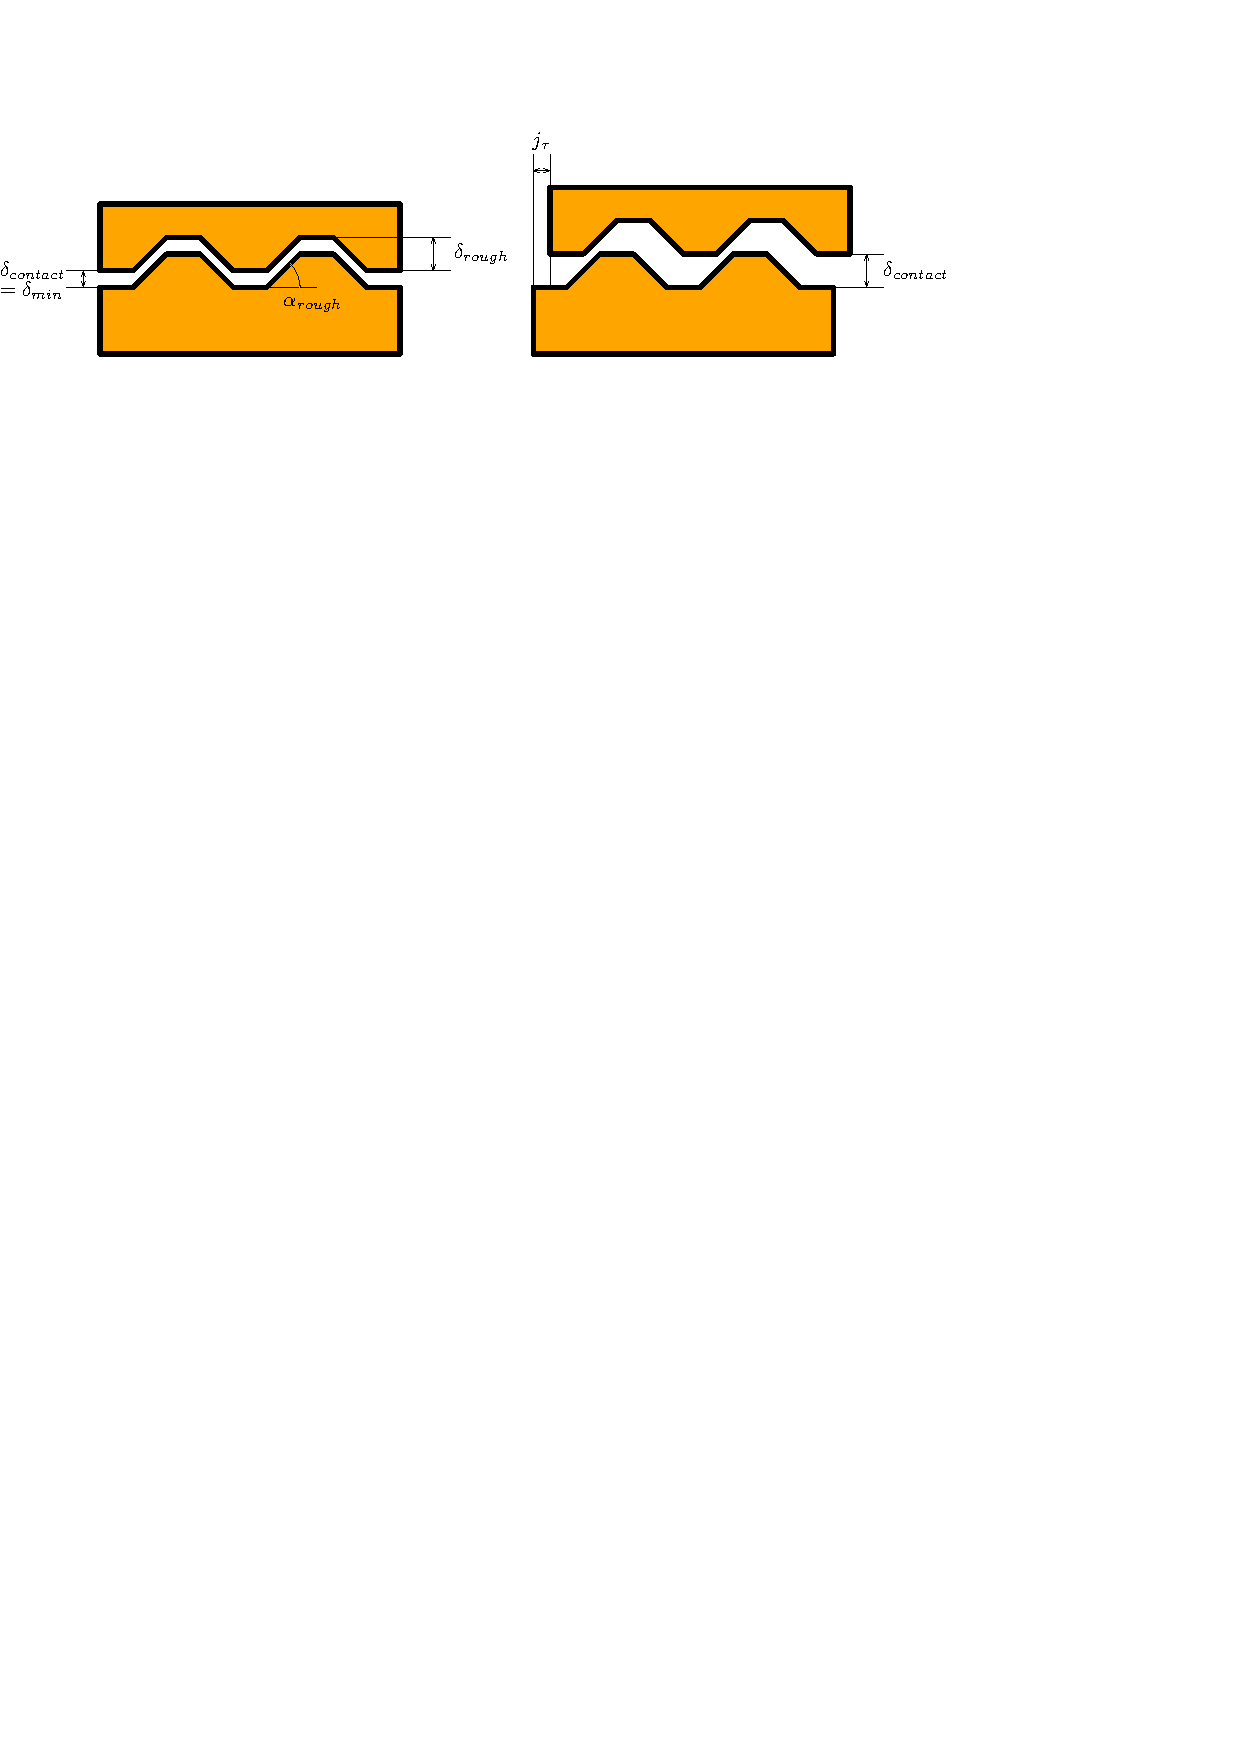
\includegraphics{figures/shear_dilation}
\caption{Ilustration of shear dilation effect: The contact distance increases with tangential displacement.}
\label{fig:shear_dilation}
\end{figure}
For the case of 1d intersections of three or more 2d fractures, $j_\tau$ is generalized to the following formula:
\eq{ j_\tau = \sqrt{ \sum_{i,j=1}^n \delta^i\delta^j(\uu^i_{\tau}\cdot\uu^j_{\tau}) (\nn^i\cdot\nn^j), } }
where $\uu_{i\tau}$ is the tangential displacement on $i$-th branch.

When contact conditions are active, the mechanical model is solved as a quadratic programming problem with linear constraints.

\paragraph{Output fields.}
The mechanics equation provides several fields for output:
\begin{itemize}
    \item \hyperA{Mechanics-LinearElasticity-FE-OutputFields::displacement}{displacement}: The computed displacement vector field $\uu$;
    \item \hyperA{Mechanics-LinearElasticity-FE-OutputFields::stress}{stress}: The mechanical stress tensor $\tn\sigma(\uu)$;
    \item \hyperA{Mechanics-LinearElasticity-FE-OutputFields::mean-stress}{mean\_stress}: The mean of the principal stresses, i.e. $\sigma_m:=\frac13\tn I:\tn\sigma(\uu)$;
    \item \hyperA{Mechanics-LinearElasticity-FE-OutputFields::von-mises-stress}{von\_mises\_stress}: $\sigma_{VM}:=\sqrt{\frac32\tn\sigma_d:\tn\sigma_d}$, where $\tn\sigma_d:=\tn\sigma(\uu)-\sigma_m\tn I$ is the deviatoric stress.
    Equivalently, von Mises stress can be expressed as
    \[ \sigma_{VM} = \sqrt{\frac12\left((\sigma_1-\sigma_2)^2+(\sigma_1-\sigma_3)^2+(\sigma_2-\sigma_3)^2\right)}, \]
    where $\sigma_{1,2,3}$ are the principal stresses, i.e. eigenvalues of $\tn\sigma(\uu)$;
    \item \hyperA{Mechanics-LinearElasticity-FE-OutputFields::cross-section-updated}{cross\_section\_updated}: This field expresses the cross-section of fractures after deformation and is defined as $\delta_d-\sum_{i=1}^n\uu^i_{d+1}\cdot\nn^i_{d+1}$;
    \item \hyperA{Mechanics-LinearElasticity-FE-OutputFields::displacement-divergence}{displacement\_divergence}: $\widetilde\div\uu_d$;
    \item \hyperA{Mechanics-LinearElasticity-FE-OutputFields::normal-displacement-jump}{normal\_displacement\_jump}: Displacement jump in normal direction: $\sum_{i=1}^n\uu^i_{d+1}\cdot\nn^i_{d+1}$;
    \item \hyperA{Mechanics-LinearElasticity-FE-OutputFields::tangential-displacement-jump}{tangential\_displacement\_jump}: Displacement jump in tangential direction ($j_\tau$).
\end{itemize}





\chapter{Numerical Methods}
\label{chapter:numerical}

\input{lumped_mh}

\input{dg}

\input{reaction_term_numerical}

%\input{semchem}



\chapter{File Formats}
\label{chapter:file-formats}


In this chapter, we shall describe structure of the main input file and data formats of other input files.
In particular we briefly describe the GMSH file format used for both the computational mesh as well as for the input of general spatial data.


\section{Main Input File}
\label{sec:CONformat}

In this section, we shall describe structure of the main input file that is given either as the first positional argument or through 
the parameter \verb'-s' on the command line. First, we provide a~quick introduction to the YAML file format. Then, we demonstrate the most important 
input structures on the examples. 







\subsection{YAML basics}
YAML is a~human readable data format. It is designed to be both human readable and human editable. As it is not a~markup languages, there are
no tags to determine type of the data. The indentation and justification is used instead for data organization. Moreover the used YAML format (version 1.2) is 
superset of the JSON format, another minimalist data serialization format where braces and brackets are used instead of indentation.
For the more detailed description see \href{https://en.wikipedia.org/wiki/YAML}{Wikipedia} 
for further technical details and for reference parsers for various programming languages see YAML \href{http://yaml.org/}{home page} .

\subsubsection{Hierarchy of Mappings and Lists}
Elementary data are organized to lists and mappings. Let us start with an example of a~list:
\begin{verbatim}
# Example of list 
- 3.14                  # a number
- 2014-01-14            # a date
- Simple string.        # a string
- "3 is three"          # quoting necessary
- '3 is three'          # other quoting
- true                  # boolean
\end{verbatim}
Comments are started by a~hash (\verb'#') which can appear anywhere on a~line and marks the comment up to the end of line.
The the list follows with single item per line preceded by a~dash (\verb'-'). Any value starting by a~digit is interpreted as a~number
or date. Values starting with letter is interpreted as a~string. Otherwise one may use double (\verb'""') or single (\verb"''") 
quotas to mark a~string value explicitly. Finally some strings are interpreted as Boolean values, it is recommended to use 
\verb'true' and \verb'false' (other possible pairs are e.g. \verb'yes/no', \verb'y/n', \verb'on/off'). 

Alternatively a~list may be written in compact "JSON" way enclosing the list into brackets:
\begin{verbatim}
# Compact list
[ 3.14, 2014-01-14, Simple string.,
"3 is three", '3 is three'] 
\end{verbatim}

Other data structure is called mapping, which is also known as directory or associative array:
\begin{verbatim}
# Example of a mapping
pi: 3.14
date: 2014-01-14   
name: Mr. Simple String
\end{verbatim}

Again one may use also JSON syntax with mapping enclosed in braces:
\begin{verbatim}
# Compact mapping
{ pi: 3.14, date: 2014-01-14,   
name: Mr. Simple String }
\end{verbatim}

Mappings and lists may by mutually nested:
\begin{verbatim}
list:
    - one
    - two
    - 
        - three one 
        - three two
map:
    a: one 
    b: two
\end{verbatim}

A string may be split to more lines using {\it greater then} (\verb'>') and multi-line strings may be entered after {\it vertical line} (\verb'|'):
\begin{verbatim}
# single long string
one_line: >
    Single line string
    broken into two lines.
# multi line string
multi_line: |
    First line.
    Second line.
\end{verbatim}
In the first case the line breaks are replaced by space, in the second case the line breaks are preserved.
In both cases the leading indentation is removed.


\subsubsection{Tags}
YAML format defines a~syntax for explicit specification of types of values including the types specific to an application.
The application specific tags are used by Flow123d to specify particular implementation of various algorithms or data types.
The general syntax of tags is quite complicated, so we present only the syntax used in the Flow123d input.
\begin{verbatim}
    field_a: !FieldFormula
        value: !!str "5 * x" 
    field_b:  !FieldFormula "5 * x"   
\end{verbatim}

The \verb'field_a' have specified evaluation algorithm \verb'FieldFormula', the key value have explicitly specified the default tag \verb'str'.
Note that default types are detected automatically and need not to be specified. On the third line we use even more compact way to 
express the same thing. Further details about usage of tags in Flow123d follows in Section \ref{sec:abstract}.

\subsubsection{References}
Anchors and references allows to reduce redundancy in the input data:
\begin{verbatim}
aux_name: &anchor_name John Smith
aux_man: &common_man
    sex: man
    city: Prague
    
people:
   - << *_common_man
     name: John Paul
   - << *_common_man
     name: *anchor_name
\end{verbatim}
On the first line, we define the anchor \verb'&anchor_name' for the value \verb'John Smith'. On the second line, 
we define the anchor \verb'&common_man' for the dictionary. Later, we use \verb'<<' to inject the dictionary 
referenced by \verb'*common_man'. Finally the anchor \verb'&anchor_name' is referenced by \verb'*anchor_name' to reuse the 
name \verb'John Smith'.

Ignoring the auxiliary keys \verb'aux_name' and \verb'aux_man' this is equivalent to:
\begin{verbatim}
people:
   - sex: man
     city: Prague
     name: John Paul
   - sex: man
     city: Prague
     name: John Smith
\end{verbatim}


\subsubsection{Gotchas}
\begin{itemize}
 \item Unquoted string values can not contain characters: colon \verb':', hash \verb'#', 
 brackets \verb'[]', braces \verb'{}', less then \verb'<', vertical bar \verb'|'.
 \item For indentation one can use only spaces; tabs are not allowed. However, your editor may automatically convert tabs to spaces.
 \item Boolean special strings must be quoted if you want to express a~string. This is not problem for the Flow123d input.
 \item Numbers starting with digit zero are interpreted as octal numbers. 
\end{itemize}

\subsection{Flow123d input types}
\label{sec:input_types}
Flow123d have a~subsystem for definition of the structure of the input file including preliminary checks for the 
correctness of the values. This subsystem works with elementary data types:
\begin{itemize}
 \item {\it Bool} corresponds to the YAML Boolean values
 \item {\it Double}, {\it Integer} initialized from YAML numeric values. 
 \item {\it String}, {\it FileName}, {\it Selections} initialized from YAML strings.
\end{itemize}
Numerical values have defined valid ranges. FileName values are used for reference to external files either for input or for output.
Selection type defines a~finite number of valid string values which may appear on the input. 
These elementary types are further organized into Records and Arrays in order to specify strongly typed definition of the 
input data file. Array and Records forms so called input structure tree (IST).

In order to make {\it "simple things simple and complex things possible" (Alan Kay)} the input system provides
so called {\it automatic conversions}. If the YAML type on input does not match the expected data type automatic conversion tries to convert 
the input to the expected type. Automatic conversion rules for individual composed types follows.

\subsubsection{Record (YAML Mapping, JSON object)}
A Record is initialized from the YAML mapping. However, in contrast to YAML mappings 
the Records have fixed keys with fixed types. 
This is natural as Records are used for initialization of C++ objects which 
are also strongly typed. Every Record type have unique name and have defined list of its keys.
Keys are lowercase strings without spaces, possibly using digits and underscore. Every key has
a type and default value specification. Default value specification can be:
\begin{description} 
 \item[obligatory] --- means no default value, which has to be specified at input. 
 \item[optional] --- means no default value, but value is needs not to be specified. Unspecified value usually means that you turn off some functionality.
 \item[default at declaration] --- the default value is explicitly given in declaration and is automatically provided by the input subsystem if needed
 \item[default at read time] --- the default value is provided at read time, usually from some other variable. In the documentation, 
 there is only textual description where the default value comes from.
\end{description}

Records that have all keys with default value or optional safe the single key $K$ may support autoconversion from an input of the type that match 
the type of the key $K$. For example:
\begin{verbatim}
  mesh: "mesh_file.msh"
\end{verbatim}
is converted to:
\begin{verbatim}
  mesh:
    mesh_file: "mesh_file.msh"
    regions: null
    partitioning: any_neighboring
    print_regions: false
    intersection_search: BIHsearch
\end{verbatim}
with the key \verb'regions' being optional and the last three keys having its default values. 


\subsubsection{Array (YAML List, JSON array)}
An Array is initialized from a~YAML list. But, in opposition to the YAML mapping, the values in a~single Array 
have all the same type. So the particular Array type is given by the type of its elements and a~specification of its size range.

Automatic conversion performs kind of transposition of the data. It simplifies input of the list of records (or arrays) 
with redundant structure, e.g. consider input
\begin{verbatim}
  list:
    a: [1,2)
    b: 4
    c: [5,6]
\end{verbatim}
Assuming that key \verb'list' have the type Array of Records and keys \verb'a', \verb'b', \verb'c' are all numerical scalars this input is equivalent to
\begin{verbatim}
  list:
    - a: 1
      b: 4
      c: 5
    - a: 2
      b: 4
      c: 6
\end{verbatim}
The rule works as follows, if a~key $K$ should have type Array, but some other type is on the input, 
we search through the input under the key $K$ for all Arrays $S$ standing instead of scalars.
All these arrays must have the same length $n$. Then the $i$-th element of the key $A$ array is
copy of the input keeping only $i$-th elements of the Arrays $S$.
As a~special case if there are no Arrays $S$ a~list with single element equal to the input is created.
Only this simplest conversion to an Array is applied if inappropriate type is found 
while the transposition is processed.





\subsubsection{Abstract}
\label{sec:abstract}
An Abstract type allows a~certain kind of polymorphism corresponding to a~pure abstract class in C++ or to an interface in Java. 
Every Abstract type have unique name and set of Records that implements the Abstract. The particular type must be provided on input through the YAML tag.
See description of \hyperlink{sec:Fields}{Fields} below for examples.

An Abstract type may have specified the default implementation. If this default Record supports automatic conversion from one of its keys
we can see it as an automatic conversion from that key to the Abstract. For example
\begin{verbatim}
 conductivity: 2.0
\end{verbatim}
where conductivity is of Abstract type \verb'Field' with scalar values, is in fact converted to
\begin{verbatim}
 conductivity: !FieldConstant
    value: 2.0
\end{verbatim}
as the \verb'FieldConstant' is default implementation of the field and it is auto=convertible from the key \verb'value'. 

\subsubsection{Flow123d specific tags}
\label{sec:spec_tags}
Currently just two specific tags are implemented, both allowing inclusion of data in other files.

{\bf Include other YAML file} The tag \verb'!include' can be used to read a~key value from other YAML file.
Path to the file is specified as the value of the key. A relative path is rooted in the folder of the main input file.
A particular type of an Abstract key is specified as a~composed tag \verb'!include,<TYPE>'.

Example, the main input file:
\begin{verbatim}
    flow123d_version: 2.0.0
    problem: !Coupling_Sequential
        description: Test8 - Steady flow with sources
        mesh:
            mesh_file: ../00_mesh/square_1x1_shift.msh
        flow_equation: !include,Flow_Darcy_MH
            input_darcy.yaml
\end{verbatim}
Content of \verb'input_darcy.yaml', included Record:
\begin{verbatim}
    nonlinear_solver:
        linear_solver: !Petsc
    input_fields:
        darcy_input_fields.yaml
    balance: {}
    output_stream: 
        file: ./flow.pvd
\end{verbatim}
Content of \verb'darcy_input_fields.yaml', included Array:
\begin{verbatim}
    - region: plane
        anisotropy: 1
        water_source_density: !FieldFormula
        value: 2*(1-x^2)+2*(1-y^2)
    - region: .plane_boundary
        bc_type: dirichlet
        bc_pressure: 0    
\end{verbatim}

{\bf Include general CSV data}
The custom tag \verb'include_csv' can be used to include a~table (e.g. coma separated values, CSV file) as an Array of Records. 
Every line of the input table is converted to a~single element of the Array.
The tag is followed by a~Record with several keys to specify format of the data:
\begin{description}
  \item {\bf\verb'file'} \\A valid path to a~text data file. Relative to the main input file.
  \item {\bf\verb'separator'}\\ A string of characters used as separators of the values on the single line (default is coma ",").
  Tab and space are always added. Double quotas can be used to express string values containing separators, 
  backslash can be used to escaping any character with special meaning. Consecutive row of separators is interpreted as a~single separator. 
  \item {\bf\verb'n_head_lines'}\\ Skip given number of lines at the beginning.
  \item {\bf\verb'format'}\\ An input structure of a~single element in the resulting array. Type of Abstracts must be same through 
  the whole resulting Array. String scalar values with a~placeholder \verb"'$<column>'" will be replaced by the value 
  at corresponding column in the input file.
\end{description}

Current implementation have substantial limitation as it can not be combined with auto conversions. This makes these includes
little bit verbose. For example consider this section from a~main input file:
\begin{verbatim}
    ...
    substances: [A, B]
    ...    
    input_fields:
    - region: A
      porosity: !FieldTimeFunction
        time_function: !include_csv
          values:
            file: data.txt  
            separator: " "
            n_head_lines: 1
            format: 
              time: #0
              value: #1
              
    - region: .boundary_A        
      bc_conc: 
        - !FieldTimeFunction    # Substance A
          time_function: !include_csv
            values:
              file: data.txt  
              separator: " "
              n_head_lines: 1
              format: 
                time: #0
                value: #2
        - !FieldTimeFunction    # Substance B
          time_function: !include_csv
            values:
              file: data.txt  
              separator: " "
              n_head_lines: 1
              format: 
                time: #0
                value: #3
\end{verbatim}
Content of \verb'data.txt':
\begin{verbatim}
time    porosity        bc_conc_X     bc_conc_Y
0.0     0.01            1.0           0.6
0.1     0.015           0.9           0.5
0.2     0.03            0.8           0.4
\end{verbatim}

This together will be equivalent to:
\begin{verbatim}
    input_fields:
    - region: A
      porosity: !FieldTimeFunction
        time_function: 
          - time: 0.0
            value: 0.01
          - time: 0.1
            value: 0.015
          - time: 0.2
            value: 0.03
           
    - region: .boundary_A        
      bc_conc: !FieldTimeFunction
        time_function: 
          - time: 0.0
            value: [ 1.0, 0.6]
          - time: 0.1
            value: [ 0.9, 0.5]
          - time:  0.2
            value: [ 0.8, 0.4]
\end{verbatim}

So in this particular case it would be simpler to write data directly into the main file. The include from 
the text table is efficient for the long time series.




\subsection{Input subsystem}
This section provides some implementation details about the Flow123d input subsystem. This may be helpful to better understand behavior of the program for 
some special input constructions.

\begin{figure}[!hb]
 \begin{center}
 \includegraphics[scale=0.4]{\fig/input_subsystem.pdf}
 % input_subsystem.pdf: 0x0 pixel, -2147483648dpi, 0.00x0.00 cm, bb=
 \caption{Structure of the input subsystem. HDF5 format not yet supported.}
 \label{fig:input_subsystem}
 \end{center}
\end{figure}

The input subsystem of Flow123d is designed with the aim to provide uniform initialization of 
C++ classes and data structures. The scheme of the input is depicted on Figure \ref{fig:input_subsystem}.
The structure of the input file is described by the Input Structure Tree (IST) consisting of the input objects describing 
the types discussed in the previous Section \ref{sec:input_types}. The structure of the tree mostly follows follows the structure of the computational classes.

When reading the input file, the file is first parsed by the specific format parser. Using a~common interface to the parsed data, the 
structure of the data is checked against the IST and the data are pushed into the storage tree. If the input data and IST do not match
the automatic conversions described above are applied, where appropriate.
An accessor object to the root data record is the result of the file reading. The data can be retrieved through the 
accessors which combine raw data of the storage with their meaning described in IST. The IST can be written out in the JSON format
providing the description of the input file structure. This IST file is used both for generation of the input reference in HTML and \LaTeX
formats and for the Model editor --- specialized editor for the input file that is part of the GeoMop tools currently in development.

While the recommended format of the input file is YAML the JSON format can be used as well. This may be useful in particular if the input file
should be machine generated. Although the JSON format is technically subset of the YAML format. We use separate parser and use special keys in order to
mimic tags and references supported by the YAML. The type of an abstract is specified by the key \verb'TYPE'. A reference is given by a~record with the only key 
\verb'REF' which contains a~string specifying the address of the value that should be substituted.



\section{Important Record Types of Flow123d Input}
Complete description of the input structure tree can be generated into HTML or LaTeX format. While the former one provides better interactivity 
through the hyperlinks the later one is part of this user manual. The generated documentation provides whole details for all keys, but 
it may be difficult to understand the concept of the input structures. This section is aimed to provide this higher level picture.

\subsection{Mesh Record}
\label{sec:Mesh}
The \hyperA{IT::Mesh}{mesh record} provides initialization of the computational mesh consisting of points, lines, triangles and tetrahedrons in the 3D ambient space.
Currently, we support only GMSH mesh file format \href{http://geuz.org/gmsh/doc/texinfo/gmsh.html#MSH-ASCII-file-format}{MSH ASCII}. 
The input file is provided by the key \hyperA{Mesh::mesh-file}{{\tt mesh\_file}}. The file format allows to group elements into {\it regions} 
identified by a~unique label (or by ID number). The regions with labels starting with the dot character are treated as {\it boundary regions}. 
Their elements are removed from the computational domain, however they can be used to specify boundary
conditions. Other regions are called {\it bulk regions}. Every element lies directly in just one {\it simple region} while the simple regions may be 
grouped into composed regions called also region sets. A simple region may be part of any number of composed regions.
Initial assignment of the simple regions to the elements is given by the physical groups of the input GMSH file. Further
modification of this assignment as well as creation of new simple or composed regions can be done 
through the list of operations under the key \hyperA{Mesh::regions}{{\tt regions}}. The operations are performed in the order given by the input.
Operation \hyperA{IT::From-Id}{{\tt From\_Id}} sets the name of a~simple region having only ID in the input GMSH file. Operation 
\hyperA{IT::From-Label}{{\tt From\_Label}} can rename a~simple region. Operation \hyperA{IT::From-Elements}{{\tt From\_Elements}}
assign new simple region to the given list of elements overwriting their region given by the input mesh file. Finally operations 
\hyperA{IT::Union}{{\tt Union}}, \hyperA{IT::Difference}{{\tt Difference}} and \hyperA{IT::Intersection}{{\tt Intersection}}
implements standard set operations with both simple and complex regions resulting in new composed regions.




\subsection{Input Fields}
Input of every equation contains the key \verb'input_fields' used consistently for the input of the equation parameters 
in form of general time--space dependent fields.  The input fields are organized into a~list of {\it field descriptors}, see 
e.g. \hyperA{IT::Flow-Darcy-MH-Data}{\tt Data} record, the field descriptor of the Darcy flow equation.
The field descriptor is a~Record with keys 
\hyperA{Flow-Darcy-MH-Data::time}{{\tt time}}, 
\hyperA{Flow-Darcy-MH-Data::region}{{\tt region}}, 
\hyperA{Flow-Darcy-MH-Data::rid}{{\tt rid}}
and further keys corresponding to the 
names of input fields supported by the equation. The field descriptor is used to prescribe
a change of one or more fields in particular time (key \verb'time') and on particular region given  by the name (key \verb'region', preferred way) 
or by the region id (key \verb'rid'). 
The array is processed sequentially and latter values overwrite the previous ones. Change times of a~single field must form a~non-decreasing sequence.
Changes in fields given by the fields descriptor are interpreted as discontinuous changes of the changed fields
and equations try to adopt its time stepping to match these time points. This is in contrast with changes of the field values given by
the evaluation algorithms, these are always assumed to be continuous and the time steps are not adapted. 



Example:
\begin{verbatim}
input_fields:
  - # time=0.0  - default value
    region: BULK
    conductivity: 1   # setting the conductivity field on all regions
  - region: 2d_part
    conductivity: 2  # overwriting the previous value
  - time: 1.0
    region: 2d_part
    conductivity: !FieldFormula
      # from time=1.0 we switch to the linear function in time
      value: 2+t
  - time: 2.0
    region: 2d_part
    conductivity: !FieldElementwise
      # from time=2.0 we switch to elementwise field, but only
      # on the region "2d_part"
      gmsh_file: ./input/data.msh
      field_name: conductivity
\end{verbatim}



\subsubsection{Field Algorithms}
\label{sec:Fields}\hypertarget{sec:Fields}{}

A general time and space dependent, scalar, vector, or  tensor valued function can be specified through the family of abstract records 
\verb'Field:R3 -> X', where $X$ is a~type of value returned by the field, which can be:
\begin{itemize}
 \item $T$ --- scalar valued field, with scalars of type $T$
 \item $T[d]$ --- vector valued field, with vector of fixed size $d$ and elements of type $T$
 \item $T[d, d]$ --- tensor valued field, with square tensor of fixed size and elements of type $T$
\end{itemize}
the scalar type $T$ can be one of
\begin{itemize}
 \item {\bf Real} --- scalar real valued field
 \item {\bf Int}  --- scalar integer valued field
 \item {\bf Enum} --- scalar non negative integer valued field. Values on the input are of the type Selection.
\end{itemize}

Each of these abstract records have the same set of descendants which implement various evaluation algorithms of the fields. These are
\begin{description}
 \item[FieldConstant] --- field that is constant both in space and time
 \item[TimeFunction] --- field that is constant in space and continuous in time. Values are interpolated (currently only linear interpolation) from 
 the sequence of time-value pairs provided on input.
 \item[FieldFormula] --- field that is given by runtime parsed formula using $x,y,z,t$ coordinates. The \href{http://warp.povusers.org/FunctionParser/}{Function Parser} library is used
 with syntax rules described \href{http://warp.povusers.org/FunctionParser/fparser.html#literals}{here}.
 \item[FieldPython] --- field can be implemented by Python script either specified by string (key \hyperA{FieldPython::script-string}{{\tt script\_string}}) 
 or in external file (key \hyperA{FieldPython::script-file}{{\tt script\_file}}. 
 \item[FieldElementwise] --- discrete field, currently only piecewise constant field on elements is supported, the field can given by 
 the \href{http://geuz.org/gmsh/doc/texinfo/gmsh.html#MSH-ASCII-file-format}{MSH ASCII} file specified in key \hyperA{FieldElementwise::gmsh-file}{{\tt gmsh\_file}} and field name in the file given 
 by key \hyperA{FieldElementwise::field-name}{{\tt field\_name}}. The file must contain same mesh as is used for computation.
 \item[FieldInterpolated] --- allows interpolation between different meshes. Not yet fully supported.
\end{description}

Several automatic conversions are implemented. Scalar values can be used to set constant vectors or tensors. Vector value of size $d$ can be used to set diagonal tensor $d\times d$.
Vector value of size $d(d-1)/2$, e.g. $6$ for $d=3$, can be used to set symmetric tensor. These rules apply only for FieldConstant and FieldFormula.
Moreover, all Field abstract types have default value \verb'TYPE=FieldConstant'. Thus you can just use the constant value instead of the whole record.

Examples:
\begin{verbatim}
input fields:
   - conductivity: 1.0
     # is equivalent to
   - conductivity: !FieldConstant
        value=1.0
   
   - anisotropy: [1 ,2, 3] # diagonal tensor
     # is equivalent to
   - anisotropy: !FieldConstant
        value=[[1,0,0],[0,2,0],[0,0,3]]

     # concentration for 2 components   
   - conc: !FieldFormula  ["x+y", "x+z"]
     # is equivalent to
   - conc: 
       - !FieldFormula
         value: "x+y"
       - !FieldFormula
         value: "x+z"
\end{verbatim}

\subsubsection{Field Units}
Every field (e.g. conductivity or storativity) have specified unit in terms of powers of the base SI units. 
The user, however, may set input in different units specified by the key \verb'unit' 
supported by every field algorithm. The key have type \hyperA{IT::Unit}{\tt Unit} record, auto convertible from its only key 
\verb'unit_formula' of the string type. Effectively the \hyperA{IT::Unit}{\tt Unit} is a string with particular syntax. 
The unit formula is evaluated  into a~coefficient and an SI unit. The resulting SI unit 
must match expected SI unit of the field, while the input value 
of the field (including values from external files or returned by Python functions)  
is multiplied by the coefficient before further processing.

The syntax of unit formula is: {\tt <UnitExpr>;<Variable>=<Number>*<UnitExpr>;...,}
where {\tt <Variable>} is a~variable name and {\tt <UnitExpr>} is a~units expression
which consists of products and divisions of terms, where a~term has form \verb'<Base>^<N>', 
where {\tt <N>} is an integer exponent and {\tt <Base>} is either a~base SI unit, 
a derived unit, or a~variable defined in the same unit formula.
Example, unit for the pressure head: 
\begin{verbatim}
   pressure_head: !FieldConstant      # [m] expected
     value: 100                       # [MPa] 
     unit:  MPa/rho/g_; rho = 990*kg*m^-3; g_ = 9.8*m*s^-2     
\end{verbatim}

Standard single letter prefixes: a,f,p,n,u,m,d,c,h,k,M,G,T,P,E\\
are supported for the basic SI units: m,g,s,A,K,cd,mol\\
and for the derived SI units: N, J, W, Pa, C, D, l.

Moreover several specific units are supported: 
t = 1000 kg
min = 60 s 
h = 60 min
d = 24 h
y = 365.2425 d




\subsection{Output Records}
Output from the models is controlled by an interplay of following records: \hyperA{IT::OutputStream}{{\tt OutputStream}},
\hyperA{IT::Balance}{{\tt Balance}}, and \hyperA{IT::EquationOutput}{{\tt EquationOutput}}. The first two are part of the 
records of so called {\it balance equations} which provides complete description of some balanced quantity. 
Every such equation have its own balance output controlled by the \verb'Balance' record and its own output stream for the 
spatial data controlled by the \verb'OutputStream' record. Further every equation with its own output fields 
(every input field is also output field) have the \verb'EquationOutput' record to setup output of its fields.

\subsubsection{Balance}
The balance output is performed in times given by the key \hyperA{Balance::times}{{\tt times}}
with type \verb'TimeGrid' described \hyperlink{sec:TimeGrid}{below}. Setting the key \hyperA{Balance::add-output-times}{{\tt add\_output\_times}} 
to \verb'true' the set of balance output times is enriched by the output times of the output stream of the same equation.

\subsubsection{OutputStream}
Set the file format of the output stream, possibly setting the output name, however the default value for the file name is preferred and the corresponding key 
\hyperA{OutputStream::file}{{\tt file}} is obsolete.
The time set provided by the optional key \hyperA{OutputStream::times}{{\tt times}} is used as a~default time set for a~similar key in associated 
\verb'EquationOutput' records. Finally, the key \hyperA{OutputStream::observe-points}{{\tt observe\_points}} is used to specify observation points
in which the associated equation output evaluates the observed fields.

\subsubsection{EquationOuput}
The output of the fields can be done in two ways: full spatial information saved only at selected time points in form of 
VTU or GMSH file, or full temporal information saved for every computational time, but only in selected output points.
The list of fields for spatial output is given by key \hyperA{EquationOutput::fields}{{\tt fields}} while the fields 
evaluated in the observation points are selected by the key \hyperA{EquationOutput::observe-fields}{{\tt observe\_fields}}.
The outputs times for the spatial output can be selected individually for every field in the 
\hyperA{EquationOutput::fields}{{\tt fields}} however the default list of output times is given by the key
\hyperA{EquationOutput::times}{{\tt times}} which can by optionally extended by the list of input times
using the key \hyperA{EquationOutput::add-input-times}{{\tt add\_input\_times}}.

\subsubsection{TimeGrid Array}
\hypertarget{sec:TimeGrid}{}

An array of the \hyperA{IT::TimeGrid}{{\tt TimeGrid}} records may be used to setup a~sequence of times. Such sequence is used in particular 
to trigger various types of output. A single TimeGrid represents a~regular grid of times with given start time, end time and step.


% Copyright (C) 2007 Technical University of Liberec.  All rights reserved.
%
% Please make a following refer to Flow123d on your project site if you use the program for any purpose,
% especially for academic research:
% Flow123d, Research Centre: Advanced Remedial Technologies, Technical University of Liberec, Czech Republic
%
% This program is free software; you can redistribute it and/or modify it under the terms
% of the GNU General Public License version 3 as published by the Free Software Foundation.
%
% This program is distributed in the hope that it will be useful, but WITHOUT ANY WARRANTY;
% without even the implied warranty of MERCHANTABILITY or FITNESS FOR A PARTICULAR PURPOSE.
% See the GNU General Public License for more details.
%
% You should have received a copy of the GNU General Public License along with this program; if not,
% write to the Free Software Foundation, Inc., 59 Temple Place - Suite 330, Boston, MA 021110-1307, USA.


\section{Mesh and Data File Format MSH ASCII}
\label{mesh_file}

Currently, the only supported format for the computational mesh is MSH ASCII format in version 2 used
by the GMSH software described as a 
\href{http://gmsh.info//doc/texinfo/gmsh.html#MSH-file-format-version-2-_0028Legacy_0029}{legacy format}.
Same format can be used for the FieldFE data. Support for the new version 4 format is planed for the version 4.0.0 of Flow123d.

The scheme of the file is as follows:
\begin{verbatim}
$MeshFormat
<format version>
$EndMeshFormat

$PhysicalNames
<number of items>
<dimension>     <region ID>     <region label>
...
$EndPhysicalNames

$Nodes
<number of nodes>
<node ID> <X coord> <Y coord> <Z coord>
...
$EndNodes

$Elements
<number of elements>
<element ID> <element shape> <n of tags> <tags> <nodes>
...
$EndElements

$ElementData
<n of string tags>
    <field name>
    <interpolation scheme>
<n of double tags>
    <time>
<n of integer tags>
    <time step index>
    <n of components>
    <n of items>
    <partition index>
<element ID> <component 1> <component 2> ...
...
$EndElementData
\end{verbatim}
Detailed description of individual sections:
\begin{description}
 \item[{\tt PhysicalNames}] : Assign labels to region IDs. Elements of one region should have common dimension. 
    Flow123d interprets regions with labels starting with period as the boundary elements that are not used for calculations.
 \item[{\tt Nodes}] : {\tt <number of nodes>} is also number of data lines that follows. 
    Node IDs are unique but need not to form an arithmetic sequence. Coordinates are float numbers.
 \item[{\tt Elements}] : Element IDs are unique but need not to form an arithmetic sequence. 
    Integer code {\tt <element shape>} represents the shape of element, we support only points (15), lines (1), triangles (2), and tetrahedrons (4).
    Default number of tags is 3. The first is the region ID, the second is ID of the geometrical entity (that was used in original geometry file from which the mesh was generated),
    and the third tag is the partition number. {\tt nodes} is list of node IDs with size according to the element shape.
 \item[{\tt ElementData}] : The header has 2 string tags, 1 double tag, and 4 integer tags with default meaning. For the purpose of the \verb'FieldElementwise' the tags
    \verb'<field name>', \verb'<n of components>', and \verb'<n of items>' are obligatory. This header is followed by field data on individual elements. 
    Flow123d assumes that elements are sorted by {\tt element ID}, but doesn't need to form a~continuous sequence.
\end{description}


%%%%%%%%%%%%%%%%%%%%%%%%%%%%%%%%%%%%%%%%%%%%%%%%%%%%%%%%%%%%%%%%%%%%%%%%%%%%%%%%%%%%%%%%%%%%%


% Copyright (C) 2007 Technical University of Liberec.  All rights reserved.
%
% Please make a following refer to Flow123d on your project site if you use the program for any purpose,
% especially for academic research:
% Flow123d, Research Centre: Advanced Remedial Technologies, Technical University of Liberec, Czech Republic
%
% This program is free software; you can redistribute it and/or modify it under the terms
% of the GNU General Public License version 3 as published by the Free Software Foundation.
%
% This program is distributed in the hope that it will be useful, but WITHOUT ANY WARRANTY;
% without even the implied warranty of MERCHANTABILITY or FITNESS FOR A PARTICULAR PURPOSE.
% See the GNU General Public License for more details.
%
% You should have received a copy of the GNU General Public License along with this program; if not,
% write to the Free Software Foundation, Inc., 59 Temple Place - Suite 330, Boston, MA 021110-1307, USA.

\section{Output Files}
\label{section_output}

Flow123d supports output of scalar, vector and tensor data fields into two formats. The first is the native format of the GMSH software (usually with extension \verb'msh')
which contains computational mesh followed by data fields for sequence of time levels. The second is the XML version of VTK files. These files can be 
viewed and post-processed by several visualization software packages. However, our primal goal is to support data transfer into the Paraview visualization software.
See key \hyperA{OutputStream::format}{{\tt format}}.

Input records of most equations (flow, transport, heat, some reaction models) contain the keys {\tt output\_stream} and {\tt output}.
In {\tt output\_stream}, the name and type of the output file is specified.
Further, in {\tt output}, one determines the list of fields intended for output.
The available output fields include input data as well as the simulation results.

We mention the most important output fields of all equations and link to the complete lists in Table \ref{tab:output_fields}.

\begin{table}[!h]
    \centering
    \caption{Most important output fields.}
    \label{tab:output_fields}
    \begin{tabular}{|l|p{10cm}|}
    \hline
    \multicolumn{2}{|l|}{\bf Flow\_Darcy\_MH and Richards\_LMH}\\
    \hline
    \tt pressure\_p0 & Pressure head \units{}{1}{}, piecewise constant on every element. This field is directly produced by the MH method and thus contains no postprocessing error. \\
    \hline
    \tt velocity\_p0 & Vector field of water flux \units{}{3}{-1}. For every element we evaluate discrete flux field at barycenter.\\
    \hline
    \tt piezo\_head\_p0 & Piezometric head \units{}{1}{}, piecewise constant on every element. This is just pressure on element  plus z-coordinate of the barycenter. This field is produced only on demand
    (see key \hyperA{IT::Flow-Darcy-MH-OutputFields}{\tt piezo\_head\_p0}).\\
    \hline
    complete list & See \hyperA{IT::Flow-Darcy-MH-OutputFields}{Darcy flow output fields}.\\
    \hline
    % \end{tabular}
    % 
    % \begin{tabular}{|l|p{10cm}|}
    % \hline
    \multicolumn{2}{|l|}{\bf Solute\_Advection\_FV}\\
    \hline
    \tt conc & Concentration \units{1}{-3}{}, piecewise constant on every element.\\
    \hline
    complete list & See \hyperA{IT::Solute-Advection-FV-OutputFields}{Convection transport output fields}.\\
    \hline
    % \end{tabular}
    % 
    % \begin{tabular}{|l|p{10cm}|}
    % \hline
    \multicolumn{2}{|l|}{\bf Solute\_AdvectionDiffusion\_DG}\\
    \hline
    \tt conc & Concentration \units{1}{-3}{}, piecewise linear on every element. Even if higher order polynomial approximation is used in simulation, the results are saved only in element corners.\\
    \hline
    complete list & See \hyperA{IT::Solute-AdvectionDiffusion-DG-OutputFields}{Transport with dispersion output fields}.\\
    \hline
    % \end{tabular}
    % 
    % \begin{tabular}{|l|p{10cm}|}
    % \hline
    \multicolumn{2}{|l|}{\bf DualPorosity}\\
    \hline
    \tt conc\_immobile & Concentration \units{1}{-3}{} in immobile zone, piecewise linear on every element.\\
    \hline
    complete list & See \hyperA{IT::DualPorosity-OutputFields}{Dual porosity output fields}.\\
    \hline
    % 
    \multicolumn{2}{|l|}{\bf Sorption, SorptionMobile, SorptionImmobile}\\
    \hline
    \tt conc\_solid & Concentration [mol\,$\mathrm{kg}^{-1}$] of sorbed substance, piecewise linear on every element.\\
    \hline
    complete list & See \hyperA{IT::Sorption-OutputFields}{Sorption output fields}, 
    \hyperA{IT::SorptionMobile-OutputFields}{Mobile sorption output fields}, 
    \hyperA{IT::SorptionImmobile-OutputFields}{Immobile sorption output fields}.\\
    \hline
    % 
    \multicolumn{2}{|l|}{\bf Heat\_AdvectionDiffusion\_DG}\\
    \hline
    \tt temperature & Temperature [K], piecewise linear on every element. Even if higher order polynomial approximation is used in simulation, the results are saved only in element corners.\\
    \hline
    complete list & See \hyperA{IT::Heat-AdvectionDiffusion-DG-OutputFields}{Heat transfer output fields}.\\
    \hline
    \end{tabular}
\end{table}



% \subsection{Output data fields of water flow module}
% Water flow module provides output of four data fields. 
% \begin{description}
%  \item[pressure on elements] Pressure head in length units $[L]$ piecewise constant on every element. This field is directly produced by the MH method and thus contains no postprocessing error.
%  \item[pressure in nodes] Same pressure head field, but interpolated into $P1$ continuous scalar field. Namely you lost dicontinuities on fractures.
%  \item[velocity on elements] Vector field of water flux volume unit per time unit $[L^3 / T]$. For every element we evaluate discrete flux field in barycenter.
%  \item[piezometric head on elements] Piezometric head in length units $[L]$ piecewise constant on every element. This is just pressure on element  plus z-coordinate of the barycenter. This field is produced only on demand
%  (see key \hyperA{DarcyMHOutput::piezo-head-p0}{\tt piezo\_head\_p0}).
% \end{description}
% 
% \subsection{Output data fields of transport}
% Transport module provides output only for concentrations (in mobile phase) as a~field piecewise constant over elements. There is one field for every substance and names of those fields contain 
% names of substances given by key \hyperA{TransportOperatorSplitting::substances}{{\tt substances}}. The physical unit is mass unit over volume unit $[M / L^3]$.



%\subsection{GMSH viewer remarks}

%\subsection{Paraview viewer remarks}

\subsection{Auxiliary Output Files}

\subsubsection{Profiling Information}
On every run we collect some basic profiling information. After all computations these data are written into the file
\verb'profiler%y%m%d_%H.%M.%S.out' where \verb'%y', \verb'%m', \verb'%d', \verb'%H', \verb'%M', \verb'%S' are 
two digit numbers representing year, month, day, hour, minute, and second of the program start time.

\subsubsection{Balance of Conservative Quantities}\label{sec:balance_output}
Primary and secondary equations can produce additional information on fluxes, sources and state of conservative quantities (for flow it is the volume of water, for transport the mass of a~substance, for heat transfer the energy).
The computation of balance is governed by the key \verb'balance'.
The balance file (default \verb'water_balance.txt', \verb'mass_balance.txt', \verb'energy_balance.txt') contains the following information:
\begin{itemize}
\item \texttt{time}
\item \texttt{region}
\item \texttt{quantity [unit]}: name and unit of the conservative quantity
\item \texttt{flux}, \texttt{flux\_in}, \texttt{flux\_out}: flux through boundary regions (positive value stands for flux into the domain)
\item \texttt{mass}: current mass in bulk regions
\item \texttt{source}, \texttt{source\_in}, \texttt{source\_out}: volume source in bulk regions, its positive and negative part 
\end{itemize}
In addition, the following values for cumulative balance are shown when \texttt{region} is \texttt{ALL}:
\begin{itemize}
\item \texttt{flux\_increment}, \texttt{source\_increment}: flux and source increment since the last balance time
\item \texttt{flux\_cumulative}, \texttt{source\_cumulative}: cumulative flux and source from the initial time
\item \texttt{error}: current mass $-$ (initial mass + cumulative sources + cumulative fluxes)
\end{itemize}


\subsubsection{Raw Water Flow Data File}
You can force Flow123d to write raw data about results of MH method. The file format is:
\begin{verbatim}
$FlowField
T=<time>
<number of elements>
<eid> <pressure> <flux x> <flux y> <flux z> <number of sides> <pressures on sides> <fluxes on sides> 
...
$EndFlowField
\end{verbatim}

where 
\begin{description}
 \item \verb'<time>' --- is simulation time of the raw output.
 \item \verb'<number of elements>' --- is number of elements in mesh, which is same as number of subsequent lines.
 \item \verb'<eid>' --- element id same as in the input mesh.
 \item \verb'<flux x,y,z>' --- components of water flux interpolated to barycenter of the element
 \item \verb'<number of sides>' --- number of sides of the element, influence number of remaining values
 \item \verb'<pressures on sides>' --- for every side average of the pressure over the side
 \item \verb'<fluxes on sides>' --- for ever side total flux through the side 
\end{description}

The side values are reported according to the side order, with sides numbering given by Table \ref{tab:side-numbers}.
\begin{table}[!h]
    \centering
    \caption{Side numbering relative to vertices.}
    \label{tab:side-numbers}
    \begin{tabular}{ccl}
        \toprule
        element dimension   &   side       &   vertices \\
        \toprule
        \multirow{2}{*}{1}  &   0          &   0  \\
                            &   1          &   1  \\
        \midrule
        \multirow{3}{*}{2}  &   0          &   0 1  \\
                            &   1          &   0 2  \\
                            &   2          &   1 2  \\    
        \midrule
        \multirow{4}{*}{3}  &   0          &   0 1 2 \\
                            &   1          &   0 1 3 \\
                            &   2          &   0 2 3 \\
                            &   3          &   1 2 3 \\    
        \bottomrule
    \end{tabular}    
\end{table}



% TODO: Update description of tests
% \chapter{Test and tutorial problems (WORK IN PROGRESS)}
%  \label{chapter:tests}
%  \input{tests}
% 
%  \chapter{Comparision of versions (WORK IN PROGRESS)}
%  \label{chapter:version_comparision}
%  \input{version_comparision}

\chapter{Tutorials}
\label{chapter:tutorials}
\input{tutorial_new}

\chapter{Main Input File Reference}
\label{chapter:input-tree-reference}
% support macros
This chapter contains generated reference to the main input file. Described types are ordered according to the 
deep first search of the input structure tree which somehow keep description of related types close to each other.
Interactive links allows passing through the tree structure in top-bottom manner. 

Ranges of arrays, integers and doubles use following notation: \verb'INT' for maximum of a~signed 32-bit integer ($\approx 2.147\times 10^9$), 
\verb'UINT' for maximum of unsigned 32-bit integer ($\approx 4.295\times 10^9$), and
\verb'inf' for maximum of the double precision floating point number ($\approx1.798\times 10^{308}$). 
\pagebreak

% generated file
\begin{RecordType}
	{IT::Root}
	{Root}
	{}% implements
	{}% reducible to key
	{{{Root record of JSON input for Flow123d.}% 
}}
		\RecKey
			{Root::flow123d-version}
			{flow123d{\_}version}
			{{String}}{}
			{ \it{Obligatory}}
			{{{Version of Flow123d for which the input file was created.
Flow123d only warn about version incompatibility.
However, external tools may use this information to provide conversion of the input file to the structure required by another version of Flow123d.}% 
}}
		\RecKey
			{Root::problem}
			{problem}
			{{abstract: }\TypeLink{IT::Coupling-Base}{Coupling{\_}Base}}{}
			{ \it{Obligatory}}
			{{{Simulation problem to be solved.}% 
}}
		\RecKey
			{Root::pause-after-run}
			{pause{\_}after{\_}run}
			{{Bool}}{}
			{ \ValueDefault{false}}
			{{{If true, the program will wait for key press before it terminates.}% 
}}
\end{RecordType}
\begin{AbstractType}
	{IT::Coupling-Base}
	{Coupling{\_}Base}
	{}
	{{{The root record of description of particular the problem to solve.}% 
}}
		\Descendant{\TypeLink{IT::Coupling-Sequential}{Coupling{\_}Sequential}}% 
\end{AbstractType}
\begin{RecordType}
	{IT::Coupling-Sequential}
	{Coupling{\_}Sequential}
	{\TypeLink{IT::Coupling-Base}{Coupling{\_}Base}}% implements
	{}% reducible to key
	{{{Record with data for a general sequential coupling.}% 
}}
		\RecKey
			{Coupling-Sequential::time}
			{time}
			{{record: }\TypeLink{IT::TimeGovernor}{TimeGovernor}}{}
			{ \ValueDefault{{\{}{\}}}}
			{{{Time governor setting.}% 
}}
		\RecKey
			{Coupling-Sequential::description}
			{description}
			{{String}}{}
			{ \it{Optional}}
			{{{Short description of the solved problem.}\\{
Is displayed in the main log, and possibly in other text output files.}% 
}}
		\RecKey
			{Coupling-Sequential::mesh}
			{mesh}
			{{record: }\TypeLink{IT::Mesh}{Mesh}}{}
			{ \it{Obligatory}}
			{{{Computational mesh common to all equations.}% 
}}
		\RecKey
			{Coupling-Sequential::flow-equation}
			{flow{\_}equation}
			{{abstract: }\TypeLink{IT::DarcyFlow}{DarcyFlow}}{}
			{ \it{Obligatory}}
			{{{Flow equation, provides the velocity field as a result.}% 
}}
		\RecKey
			{Coupling-Sequential::solute-equation}
			{solute{\_}equation}
			{{abstract: }\TypeLink{IT::AdvectionProcess}{AdvectionProcess}}{}
			{ \it{Optional}}
			{{{Transport of soluted substances, depends on the velocity field from a Flow equation.}% 
}}
		\RecKey
			{Coupling-Sequential::heat-equation}
			{heat{\_}equation}
			{{abstract: }\TypeLink{IT::AdvectionProcess}{AdvectionProcess}}{}
			{ \it{Optional}}
			{{{Heat transfer, depends on the velocity field from a Flow equation.}% 
}}
\end{RecordType}
\begin{RecordType}
	{IT::TimeGovernor}
	{TimeGovernor}
	{}% implements
	{\TypeLink{TimeGovernor::max-dt}{max{\_}dt}}% reducible to key
	{{{Time axis settings of the simulation.}\\{
The settings is specific to a particular equation.}\\{
TimeGovernor allows to:}\\{
 - define start time and end time of simulation}\\{
 - define lower and upper limits of time steps}\\{
 - direct fixed time marks of whole simulation}\\{
 - set global time unit of equation (see 'common{\_}time{\_}unit' key)}\\{
Limits of time steps are defined by keys 'min{\_}dt', 'max{\_}dt', 'init{\_}dt' and 'dt{\_}limits'. Key 'init{\_}dt' has the highest priority and allows set fix size of time steps.
Pair of keys 'min{\_}dt' and 'max{\_}dt' define interval of time steps.
Both previous cases ('init{\_}dt' or pair 'min{\_}dt' and 'max{\_}dt') set global limits of whole simulation.
In contrasts, 'dt{\_}limits' allow set time-dependent function of min{\_}dt/max{\_}dt.
Used time steps of simulation can be printed to YAML output file (see 'write{\_}used{\_}timesteps'.}\\{
Fixed time marks define exact values of time steps.
They are defined in:}\\{
 - start time and end time of simulation}\\{
 - output times printed to output mesh file}\\{
 - times defined in 'dt{\_}limits' table (optional, see 'add{\_}dt{\_}limits{\_}time{\_}marks' key)}% 
}}
		\RecKey
			{TimeGovernor::start-time}
			{start{\_}time}
			{{tuple: }\TypeLink{IT::TimeValue}{TimeValue}}{}
			{ \ValueDefault{0.0}}
			{{{Start time of the simulation.}% 
}}
		\RecKey
			{TimeGovernor::end-time}
			{end{\_}time}
			{{tuple: }\TypeLink{IT::TimeValue}{TimeValue}}{}
			{ \ValueDefault{5e+17}}
			{{{End time of the simulation.}\\{
The default value is higher than the age of the Universe (given in seconds).}% 
}}
		\RecKey
			{TimeGovernor::init-dt}
			{init{\_}dt}
			{{tuple: }\TypeLink{IT::TimeValue-2}{TimeValue}}{}
			{ \ValueDefault{0.0}}
			{{{Initial guess for the time step.}\\{
It applies to equations that use an adaptive time stepping.
If set to 0.0, the time step is determined in fully autonomous way, assuming the equation supports it.}% 
}}
		\RecKey
			{TimeGovernor::min-dt}
			{min{\_}dt}
			{{tuple: }\TypeLink{IT::TimeValue-2}{TimeValue}}{}
			{implicit value: "{Machine precision.}"}
			{{{Soft lower limit for the time step.}\\{
Equation using an adaptive time stepping cannot suggest smaller time step.
The actual time step can only decrease below the limit in order to match the prescribed input or output times.}% 
}}
		\RecKey
			{TimeGovernor::max-dt}
			{max{\_}dt}
			{{tuple: }\TypeLink{IT::TimeValue-2}{TimeValue}}{}
			{implicit value: "{Whole time of the simulation if specified, infinity else.}"}
			{{{Hard upper limit for the time step.}\\{
The actual time step can only increase above the limit in order to match the prescribed input or output times.}% 
}}
		\RecKey
			{TimeGovernor::dt-limits}
			{dt{\_}limits}
			{{array [0, UINT] of }{tuple: }\TypeLink{IT::DtLimits}{DtLimits}}{}
			{ \it{Optional}}
			{{{Allow to set a time dependent changes in }\begin{ttfamily}min{\_}dt\end{ttfamily}{ and }\begin{ttfamily}max{\_}dt\end{ttfamily}{ limits.
This list is processed at individual times overwriting previous values of }\begin{ttfamily}min{\_}dt\end{ttfamily}{/}\begin{ttfamily}max{\_}dt\end{ttfamily}{. Limits equal to 0 are ignored and replaced with }\begin{ttfamily}min{\_}dt\end{ttfamily}{/}\begin{ttfamily}max{\_}dt\end{ttfamily}{ values.}% 
}}
		\RecKey
			{TimeGovernor::add-dt-limits-time-marks}
			{add{\_}dt{\_}limits{\_}time{\_}marks}
			{{Bool}}{}
			{ \ValueDefault{false}}
			{{{Add all times defined in }\begin{ttfamily}dt{\_}limits\end{ttfamily}{ table to the list of fixed TimeMarks.}% 
}}
		\RecKey
			{TimeGovernor::write-used-timesteps}
			{write{\_}used{\_}timesteps}
			{{Filename}}{}
			{ \it{Optional}}
			{{{Write used time steps to the given file in YAML format corresponding with the format of }\begin{ttfamily}dt{\_}limits\end{ttfamily}{.}% 
}}
		\RecKey
			{TimeGovernor::common-time-unit}
			{common{\_}time{\_}unit}
			{{record: }\TypeLink{IT::Unit}{Unit}}{}
			{ \ValueDefault{"s"}}
			{{{Common time unit of the equation.}\\{
This unit will be used for all time inputs and outputs within the equation.
Individually, the common time unit can be overwritten for every declared time.}\\{
Time units are used in the following cases:}\\{
1) Time units of time value keys in: TimeGovernor, FieldDescriptors.}\\{
   The common time unit can be overwritten for every declared time.}\\{
2) Time units in: }\\{
   a) input fields: FieldFE and FieldTimeFunction}\\{
   b) time steps definition of OutputTimeSet}\\{
   Common time unit can be overwritten by one unit value for every whole mesh data file or time function.}\\{
3) Time units in output files: observation times, balance times, frame times of VTK and GMSH}\\{
   Common time unit cannot be overwritten in these cases.}% 
}}
\end{RecordType}
\begin{TupleType}
	{IT::TimeValue}
	{TimeValue}
	{}% implements
	{\TypeLink{TimeValue::time}{time}}% reducible to key
	{{{A time with optional unit specification.}% 
}}
		\RecKey
			{TimeValue::time}
			{time}
			{{Double (-inf, +inf)}}{}
			{ \it{Obligatory}}
			{{{The time value.}% 
}}
		\RecKey
			{TimeValue::unit}
			{unit}
			{{record: }\TypeLink{IT::Unit}{Unit}}{}
			{implicit value: "{Common time unit of the equation's Time Governor.
See the key 'common{\_}time{\_}unit'.}"}
			{{{{Predefined units include: }\begin{ttfamily}s\end{ttfamily}{ seconds, }\begin{ttfamily}min\end{ttfamily}{ minutes, }\begin{ttfamily}h\end{ttfamily}{ hours, }\begin{ttfamily}d\end{ttfamily}{ days, }\begin{ttfamily}y\end{ttfamily}{ years.}\\{
The default time unit is set from the equation's time governor, see the key }\begin{ttfamily}common{\_}time{\_}unit\end{ttfamily}{in the equation's time record.}
% 
}{{User can benefit from the Unit Convertor funcionality and create different time units.}\\{
Year length example considering leap years (Gregorian calendar): }\begin{ttfamily}year; year = 365.2425*d\end{ttfamily}{.}\\{
Miliseconds example : }\begin{ttfamily}milisec; milisec = 0.001*s\end{ttfamily}{.}% 
}}}
\end{TupleType}
\begin{RecordType}
	{IT::Unit}
	{Unit}
	{}% implements
	{\TypeLink{Unit::unit-formula}{unit{\_}formula}}% reducible to key
	{{{{Specify the unit of an input value.
Evaluation of the unit formula results into a coeficient and a unit in terms of powers of base SI units.
The unit must match theexpected SI unit of the value, while the value provided on the input is multiplied by the coefficient before further processing.
The unit formula have a form:}\\
\begin{ttfamily}{\textless}UnitExpr{\textgreater};{\textless}Variable{\textgreater}={\textless}Number{\textgreater}*{\textless}UnitExpr{\textgreater};...,\end{ttfamily}\\{
where }\begin{ttfamily}{\textless}Variable{\textgreater}\end{ttfamily}{ is a variable name and }\begin{ttfamily}{\textless}UnitExpr{\textgreater}\end{ttfamily}{ is a units expression which consists of products and divisions of terms.}
% 
}{{A term has a form: }\begin{ttfamily}{\textless}Base{\textgreater}{\^{}}{\textless}N{\textgreater}\end{ttfamily}{, where }\begin{ttfamily}{\textless}N{\textgreater}\end{ttfamily}{ is an integer exponent and }\begin{ttfamily}{\textless}Base{\textgreater}\end{ttfamily}{ is either a base SI unit, a derived unit, or a variable defined in the same unit formula.
Example, unit for the pressure head:}
% 
}{{}\begin{ttfamily}MPa/rho/g{\_}; rho = 990*kg*m{\^{}}-3; g{\_} = 9.8*m*s{\^{}}-2\end{ttfamily}% 
}}}
		\RecKey
			{Unit::unit-formula}
			{unit{\_}formula}
			{{String}}{}
			{ \it{Obligatory}}
			{{{Definition of unit.}% 
}}
\end{RecordType}
\begin{TupleType}
	{IT::TimeValue-2}
	{TimeValue}
	{}% implements
	{\TypeLink{TimeValue-2::time}{time}}% reducible to key
	{{{A time with optional unit specification.}% 
}}
		\RecKey
			{TimeValue-2::time}
			{time}
			{{Double [0, +inf)}}{}
			{ \it{Obligatory}}
			{{{The time value.}% 
}}
		\RecKey
			{TimeValue-2::unit}
			{unit}
			{{record: }\TypeLink{IT::Unit}{Unit}}{}
			{implicit value: "{Common time unit of the equation's Time Governor.
See the key 'common{\_}time{\_}unit'.}"}
			{{{{Predefined units include: }\begin{ttfamily}s\end{ttfamily}{ seconds, }\begin{ttfamily}min\end{ttfamily}{ minutes, }\begin{ttfamily}h\end{ttfamily}{ hours, }\begin{ttfamily}d\end{ttfamily}{ days, }\begin{ttfamily}y\end{ttfamily}{ years.}\\{
The default time unit is set from the equation's time governor, see the key }\begin{ttfamily}common{\_}time{\_}unit\end{ttfamily}{in the equation's time record.}
% 
}{{User can benefit from the Unit Convertor funcionality and create different time units.}\\{
Year length example considering leap years (Gregorian calendar): }\begin{ttfamily}year; year = 365.2425*d\end{ttfamily}{.}\\{
Miliseconds example : }\begin{ttfamily}milisec; milisec = 0.001*s\end{ttfamily}{.}% 
}}}
\end{TupleType}
\begin{TupleType}
	{IT::DtLimits}
	{DtLimits}
	{}% implements
	{\TypeLink{DtLimits::time}{time}}% reducible to key
	{{{Time dependent changes in min{\_}dt and max{\_}dt limits.}% 
}}
		\RecKey
			{DtLimits::time}
			{time}
			{{tuple: }\TypeLink{IT::TimeValue}{TimeValue}}{}
			{ \it{Obligatory}}
			{{{The start time of dt step set.}% 
}}
		\RecKey
			{DtLimits::min-dt}
			{min{\_}dt}
			{{tuple: }\TypeLink{IT::TimeValue}{TimeValue}}{}
			{implicit value: "{'min{\_}dt' value of TimeGovernor.}"}
			{{{Soft lower limit for the time step.}% 
}}
		\RecKey
			{DtLimits::max-dt}
			{max{\_}dt}
			{{tuple: }\TypeLink{IT::TimeValue}{TimeValue}}{}
			{implicit value: "{'max{\_}dt' value of TimeGovernor.}"}
			{{{Whole time of the simulation if specified, infinity else.}% 
}}
\end{TupleType}
\begin{RecordType}
	{IT::Mesh}
	{Mesh}
	{}% implements
	{\TypeLink{Mesh::mesh-file}{mesh{\_}file}}% reducible to key
	{{{Record with mesh related data.}% 
}}
		\RecKey
			{Mesh::mesh-file}
			{mesh{\_}file}
			{{Filename}}{}
			{ \it{Obligatory}}
			{{{Input file with mesh description.}% 
}}
		\RecKey
			{Mesh::regions}
			{regions}
			{{array [0, UINT] of }{abstract: }\TypeLink{IT::Region}{Region}}{}
			{ \it{Optional}}
			{{{{List of additional region and region set definitions not contained in the mesh.
There are three region sets implicitly defined:}
% 
}
\begin{itemize}
\item {ALL (all regions of the mesh)}
\item {.BOUNDARY (all boundary regions)}
\item {BULK (all bulk regions)}
\end{itemize}
}}
		\RecKey
			{Mesh::partitioning}
			{partitioning}
			{{record: }\TypeLink{IT::Partition}{Partition}}{}
			{ \ValueDefault{"any{\_}neighboring"}}
			{{{Parameters of mesh partitioning algorithms.}% 
}}
		\RecKey
			{Mesh::print-regions}
			{print{\_}regions}
			{{Bool}}{}
			{ \ValueDefault{true}}
			{{{If true, print table of all used regions.}% 
}}
		\RecKey
			{Mesh::intersection-search}
			{intersection{\_}search}
			{{selection: }\TypeLink{IT::Types-of-search-algorithm-for-finding-intersection-candidates-}{Types of search algorithm for finding intersection candidates.}}{}
			{ \ValueDefault{"BIHsearch"}}
			{{{Search algorithm for element intersections.}% 
}}
		\RecKey
			{Mesh::global-snap-radius}
			{global{\_}snap{\_}radius}
			{{Double [0, +inf)}}{}
			{ \ValueDefault{0.001}}
			{{{Maximal snapping distance from the mesh in various search operations.
In particular, it is used to find the closest mesh element of an observe point; and in FieldFormula to find closest surface element in plan view (Z projection).}% 
}}
		\RecKey
			{Mesh::raw-ngh-output}
			{raw{\_}ngh{\_}output}
			{{Filename}}{}
			{ \it{Optional}}
			{{{Output file with neighboring data from mesh.}% 
}}
		\RecKey
			{Mesh::optimize-mesh}
			{optimize{\_}mesh}
			{{Bool}}{}
			{ \ValueDefault{true}}
			{{{If true, make optimization of nodes and elements order.
This will speed up the calculations in assembations.}% 
}}
\end{RecordType}
\begin{AbstractType}
	{IT::Region}
	{Region}
	{}
	{{{Abstract record for Region.}% 
}}
		\Descendant{\TypeLink{IT::From-Id}{From{\_}Id}}% 
		\Descendant{\TypeLink{IT::From-Label}{From{\_}Label}}% 
		\Descendant{\TypeLink{IT::From-Elements}{From{\_}Elements}}% 
		\Descendant{\TypeLink{IT::Union}{Union}}% 
		\Descendant{\TypeLink{IT::Difference}{Difference}}% 
		\Descendant{\TypeLink{IT::Intersection}{Intersection}}% 
\end{AbstractType}
\begin{RecordType}
	{IT::From-Id}
	{From{\_}Id}
	{\TypeLink{IT::Region}{Region}}% implements
	{}% reducible to key
	{{{Elementary region declared by its id.}\\{
It allows to create a new region with given id and name, or to rename an existing region of given id.}% 
}}
		\RecKey
			{From-Id::name}
			{name}
			{{String}}{}
			{ \it{Obligatory}}
			{{{Name (label) of the region.
It has to be unique per single mesh.}% 
}}
		\RecKey
			{From-Id::id}
			{id}
			{{Integer [0, INT]}}{}
			{ \it{Obligatory}}
			{{{Id of the region to which you assign the name.}% 
}}
		\RecKey
			{From-Id::dim}
			{dim}
			{{Integer [0, INT]}}{}
			{ \it{Optional}}
			{{{Dimension of the region to which you assign the name.}\\{
The value is taken into account only if a new region is created.}% 
}}
\end{RecordType}
\begin{RecordType}
	{IT::From-Label}
	{From{\_}Label}
	{\TypeLink{IT::Region}{Region}}% implements
	{}% reducible to key
	{{{Elementary region declared by its name (label).}\\{
It gives a new name to an elementary region with the original name (in the mesh file) given by the }\begin{ttfamily}mesh{\_}label.\end{ttfamily}% 
}}
		\RecKey
			{From-Label::name}
			{name}
			{{String}}{}
			{ \it{Obligatory}}
			{{{New name (label) of the region.
It has to be unique per single mesh.}% 
}}
		\RecKey
			{From-Label::mesh-label}
			{mesh{\_}label}
			{{String}}{}
			{ \it{Obligatory}}
			{{{The original region name in the input file, e.g. a physical volume name in the GMSH format.}% 
}}
		\RecKey
			{From-Label::allow-empty}
			{allow{\_}empty}
			{{Bool}}{}
			{ \ValueDefault{false}}
			{{{If true it allows to the region set to be empty (no elements).}% 
}}
\end{RecordType}
\begin{RecordType}
	{IT::From-Elements}
	{From{\_}Elements}
	{\TypeLink{IT::Region}{Region}}% implements
	{}% reducible to key
	{{{Elementary region declared by a list of elements.}\\{
The new region is assigned to the list of elements specified by the key }\begin{ttfamily}element{\_}list\end{ttfamily}{.}% 
}}
		\RecKey
			{From-Elements::name}
			{name}
			{{String}}{}
			{ \it{Obligatory}}
			{{{Name (label) of the region.
It has to be unique per single mesh.}% 
}}
		\RecKey
			{From-Elements::id}
			{id}
			{{Integer [0, INT]}}{}
			{ \it{Optional}}
			{{{Id of the region.
If unset, a unique id will be generated automatically.}% 
}}
		\RecKey
			{From-Elements::element-list}
			{element{\_}list}
			{{array [1, UINT] of }{Integer [0, INT]}}{}
			{ \it{Obligatory}}
			{{{List of ids of elements.}% 
}}
\end{RecordType}
\begin{RecordType}
	{IT::Union}
	{Union}
	{\TypeLink{IT::Region}{Region}}% implements
	{}% reducible to key
	{{{Defines a new region (set) as a union of two or more regions.
The regions can be given by their names or ids or both.}% 
}}
		\RecKey
			{Union::name}
			{name}
			{{String}}{}
			{ \it{Obligatory}}
			{{{Name (label) of the new region.
It has to be unique per single mesh.}% 
}}
		\RecKey
			{Union::region-ids}
			{region{\_}ids}
			{{array [0, UINT] of }{Integer [0, INT]}}{}
			{ \it{Optional}}
			{{{List of region ids to be added to the new region set.}% 
}}
		\RecKey
			{Union::regions}
			{regions}
			{{array [0, UINT] of }{String}}{}
			{ \it{Optional}}
			{{{List of region names (labels) to be added to the new region set.}% 
}}
\end{RecordType}
\begin{RecordType}
	{IT::Difference}
	{Difference}
	{\TypeLink{IT::Region}{Region}}% implements
	{}% reducible to key
	{{{Defines a new region (set) as a difference of two regions (sets), given by their names.}% 
}}
		\RecKey
			{Difference::name}
			{name}
			{{String}}{}
			{ \it{Obligatory}}
			{{{Name (label) of the new region.
It has to be unique per single mesh.}% 
}}
		\RecKey
			{Difference::regions}
			{regions}
			{{array [2, 2] of }{String}}{}
			{ \it{Obligatory}}
			{{{List of exactly two region (set) names.}\\{
Supposing region sets r1, r2, the result includes all regions of r1 that are not in r2.}% 
}}
\end{RecordType}
\begin{RecordType}
	{IT::Intersection}
	{Intersection}
	{\TypeLink{IT::Region}{Region}}% implements
	{}% reducible to key
	{{{Defines a new region (set) as an intersection of two or more regions (sets), given by their names.}% 
}}
		\RecKey
			{Intersection::name}
			{name}
			{{String}}{}
			{ \it{Obligatory}}
			{{{Name (label) of the new region.
It has to be unique per single mesh.}% 
}}
		\RecKey
			{Intersection::regions}
			{regions}
			{{array [2, UINT] of }{String}}{}
			{ \it{Obligatory}}
			{{{List of two or more region (set) names.}% 
}}
\end{RecordType}
\begin{RecordType}
	{IT::Partition}
	{Partition}
	{}% implements
	{\TypeLink{Partition::graph-type}{graph{\_}type}}% reducible to key
	{{{Setting for various types of mesh partitioning.}% 
}}
		\RecKey
			{Partition::tool}
			{tool}
			{{selection: }\TypeLink{IT::PartTool}{PartTool}}{}
			{ \ValueDefault{"METIS"}}
			{{{Software package used for partitioning.
See corresponding selection.}% 
}}
		\RecKey
			{Partition::graph-type}
			{graph{\_}type}
			{{selection: }\TypeLink{IT::GraphType}{GraphType}}{}
			{ \ValueDefault{"any{\_}neighboring"}}
			{{{Algorithm for generating graph and its weights from a multidimensional mesh.}% 
}}
\end{RecordType}
\begin{SelectionType}
	{IT::PartTool}
	{PartTool}
	{{{Select the partitioning tool to use.}% 
}}
		\SelectionItem
			{PartTool::PETSc}
			{PETSc}
			{{{Use PETSc interface to various partitioning tools.}% 
}}
		\SelectionItem
			{PartTool::METIS}
			{METIS}
			{{{Use direct interface to Metis.}% 
}}
\end{SelectionType}
\begin{SelectionType}
	{IT::GraphType}
	{GraphType}
	{{{Different algorithms to make the sparse graph with weighted edges}\\{
from the multidimensional mesh.
Main difference is dealing with }\\{
neighboring of elements of different dimension.}% 
}}
		\SelectionItem
			{GraphType::any-neighboring}
			{any{\_}neighboring}
			{{{Add an edge for any pair of neighboring elements.}% 
}}
		\SelectionItem
			{GraphType::any-weight-lower-dim-cuts}
			{any{\_}weight{\_}lower{\_}dim{\_}cuts}
			{{{Same as before and assign higher weight to cuts of lower dimension in order to make them stick to one face.}% 
}}
		\SelectionItem
			{GraphType::same-dimension-neighboring}
			{same{\_}dimension{\_}neighboring}
			{{{Add an edge for any pair of neighboring elements of the same dimension (bad for matrix multiply).}% 
}}
\end{SelectionType}
\begin{SelectionType}
	{IT::Types-of-search-algorithm-for-finding-intersection-candidates-}
	{Types of search algorithm for finding intersection candidates.}
	{}
		\SelectionItem
			{Types-of-search-algorithm-for-finding-intersection-candidates-::BIHsearch}
			{BIHsearch}
			{{{Use BIH for finding initial candidates, then continue by prolongation.}% 
}}
		\SelectionItem
			{Types-of-search-algorithm-for-finding-intersection-candidates-::BIHonly}
			{BIHonly}
			{{{Use BIH for finding all candidates.}% 
}}
		\SelectionItem
			{Types-of-search-algorithm-for-finding-intersection-candidates-::BBsearch}
			{BBsearch}
			{{{Use bounding boxes for finding initial candidates, then continue by prolongation.}% 
}}
\end{SelectionType}
\begin{AbstractType}
	{IT::DarcyFlow}
	{DarcyFlow}
	{}
	{{{Darcy flow model.
Abstraction of various porous media flow models.}% 
}}
		\Descendant{\TypeLink{IT::Flow-Darcy-LMH}{Flow{\_}Darcy{\_}LMH}}% 
		\Descendant{\TypeLink{IT::Flow-Richards-LMH}{Flow{\_}Richards{\_}LMH}}% 
		\Descendant{\TypeLink{IT::Coupling-Iterative}{Coupling{\_}Iterative}}% 
		\Descendant{\TypeLink{IT::Flow-Darcy-MH}{Flow{\_}Darcy{\_}MH}}% 
\end{AbstractType}
\begin{RecordType}
	{IT::Flow-Darcy-LMH}
	{Flow{\_}Darcy{\_}LMH}
	{\TypeLink{IT::DarcyFlow}{DarcyFlow}}% implements
	{}% reducible to key
	{{{Lumped Mixed-Hybrid solver for saturated Darcy flow.}% 
}}
		\RecKey
			{Flow-Darcy-LMH::time}
			{time}
			{{record: }\TypeLink{IT::TimeGovernor}{TimeGovernor}}{}
			{ \ValueDefault{{\{}{\}}}}
			{{{Time governor setting.}% 
}}
		\RecKey
			{Flow-Darcy-LMH::gravity}
			{gravity}
			{{array [3, 3] of }{Double (-inf, +inf)}}{}
			{ \ValueDefault{[0, 0, -1]}}
			{{{Vector of the gravity force.
Dimensionless.}% 
}}
		\RecKey
			{Flow-Darcy-LMH::input-fields}
			{input{\_}fields}
			{{array [0, UINT] of }{record: }\TypeLink{IT::Flow-Darcy-LMH-Data}{Flow{\_}Darcy{\_}LMH{\_}Data}}{}
			{ \it{Obligatory}}
			{{{Input data for Darcy flow model.}% 
}}
		\RecKey
			{Flow-Darcy-LMH::nonlinear-solver}
			{nonlinear{\_}solver}
			{{record: }\TypeLink{IT::NonlinearSolver}{NonlinearSolver}}{}
			{ \ValueDefault{{\{}{\}}}}
			{{{Non-linear solver for MH problem.}% 
}}
		\RecKey
			{Flow-Darcy-LMH::output-stream}
			{output{\_}stream}
			{{record: }\TypeLink{IT::OutputStream}{OutputStream}}{}
			{ \ValueDefault{{\{}{\}}}}
			{{{Output stream settings.}\\{
 Specify file format, precision etc.}% 
}}
		\RecKey
			{Flow-Darcy-LMH::output}
			{output}
			{{gen. record: }\TypeLink{IT::EquationOutput}{EquationOutput}}{{output{\_}field{\_}selection}{ = }\TypeLink{IT::Flow-Darcy-LMH-OutputFields}{Flow{\_}Darcy{\_}LMH:OutputFields}}
			{ \ValueDefault{{\{}"fields": ["pressure{\_}p0", "velocity{\_}p0"]{\}}}}
			{{{Specification of output fields and output times.}% 
}}
		\RecKey
			{Flow-Darcy-LMH::output-specific}
			{output{\_}specific}
			{{gen. record: }\TypeLink{IT::Output-DarcyMHSpecific}{Output{\_}DarcyMHSpecific}}{{output{\_}field{\_}selection}{ = }\TypeLink{IT::Flow-Darcy-MH-specific-OutputFields}{Flow{\_}Darcy{\_}MH{\_}specific:OutputFields}}
			{ \it{Optional}}
			{{{Output settings specific to Darcy flow model.}\\{
Includes raw output and some experimental functionality.}% 
}}
		\RecKey
			{Flow-Darcy-LMH::balance}
			{balance}
			{{record: }\TypeLink{IT::Balance}{Balance}}{}
			{ \ValueDefault{{\{}{\}}}}
			{{{Settings for computing mass balance.}% 
}}
		\RecKey
			{Flow-Darcy-LMH::mortar-method}
			{mortar{\_}method}
			{{selection: }\TypeLink{IT::MH-MortarMethod}{MH{\_}MortarMethod}}{}
			{ \ValueDefault{"None"}}
			{{{Method for coupling Darcy flow between dimensions on incompatible meshes. [Experimental]}% 
}}
\end{RecordType}
\begin{RecordType}
	{IT::Flow-Darcy-LMH-Data}
	{Flow{\_}Darcy{\_}LMH{\_}Data}
	{}% implements
	{}% reducible to key
	{{{Record to set fields of the equation.}\\{
The fields are set only on the domain specified by one of the keys: 'region', 'rid'}\\{
and after the time given by the key 'time'. The field setting can be overridden by}\\{
 any Flow{\_}Darcy{\_}LMH{\_}Data record that comes later in the boundary data array.}% 
}}
		\RecKey
			{Flow-Darcy-LMH-Data::region}
			{region}
			{{array [1, UINT] of }{String}}{}
			{ \it{Optional}}
			{{{Labels of the regions where to set fields. }% 
}}
		\RecKey
			{Flow-Darcy-LMH-Data::rid}
			{rid}
			{{Integer [0, INT]}}{}
			{ \it{Optional}}
			{{{ID of the region where to set fields.}% 
}}
		\RecKey
			{Flow-Darcy-LMH-Data::time}
			{time}
			{{tuple: }\TypeLink{IT::TimeValue}{TimeValue}}{}
			{ \ValueDefault{0.0}}
			{{{Apply field setting in this record after this time.}\\{
These times have to form an increasing sequence.}% 
}}
		\RecKey
			{Flow-Darcy-LMH-Data::anisotropy}
			{anisotropy}
			{{gen. abstract: }\TypeLink{IT::Field-R3-to-R-3-3-}{Field{\_}R3{\_}to{\_}R[3,3]}}{{element{\_}input{\_}type}{ = }\TypeLink{IT::Double}{Double}}
			{ \it{Optional}}
			{{{Anisotropy of the conductivity tensor. }{$[-]$}% 
}}
		\RecKey
			{Flow-Darcy-LMH-Data::cross-section}
			{cross{\_}section}
			{{gen. abstract: }\TypeLink{IT::Field-R3-to-R}{Field{\_}R3{\_}to{\_}R}}{{element{\_}input{\_}type}{ = }\TypeLink{IT::Double}{Double}}
			{ \it{Optional}}
			{{{Complement dimension parameter (cross section for 1D, thickness for 2D). }{$[m^{3-d}]$}% 
}}
		\RecKey
			{Flow-Darcy-LMH-Data::conductivity}
			{conductivity}
			{{gen. abstract: }\TypeLink{IT::Field-R3-to-R}{Field{\_}R3{\_}to{\_}R}}{{element{\_}input{\_}type}{ = }\TypeLink{IT::Double}{Double}}
			{ \it{Optional}}
			{{{Isotropic conductivity scalar. }{$[ms^{-1}]$}% 
}}
		\RecKey
			{Flow-Darcy-LMH-Data::sigma}
			{sigma}
			{{gen. abstract: }\TypeLink{IT::Field-R3-to-R}{Field{\_}R3{\_}to{\_}R}}{{element{\_}input{\_}type}{ = }\TypeLink{IT::Double}{Double}}
			{ \it{Optional}}
			{{{Transition coefficient between dimensions. }{$[-]$}% 
}}
		\RecKey
			{Flow-Darcy-LMH-Data::water-source-density}
			{water{\_}source{\_}density}
			{{gen. abstract: }\TypeLink{IT::Field-R3-to-R}{Field{\_}R3{\_}to{\_}R}}{{element{\_}input{\_}type}{ = }\TypeLink{IT::Double}{Double}}
			{ \it{Optional}}
			{{{Water source density. }{$[s^{-1}]$}% 
}}
		\RecKey
			{Flow-Darcy-LMH-Data::bc-type}
			{bc{\_}type}
			{{gen. abstract: }\TypeLink{IT::Field-R3-to-R}{Field{\_}R3{\_}to{\_}R}}{{element{\_}input{\_}type}{ = }\TypeLink{IT::Flow-Darcy-BC-Type}{Flow{\_}Darcy{\_}BC{\_}Type}}
			{ \it{Optional}}
			{{{Boundary condition type. }{$[-]$}% 
}}
		\RecKey
			{Flow-Darcy-LMH-Data::bc-pressure}
			{bc{\_}pressure}
			{{gen. abstract: }\TypeLink{IT::Field-R3-to-R}{Field{\_}R3{\_}to{\_}R}}{{element{\_}input{\_}type}{ = }\TypeLink{IT::Double}{Double}}
			{ \it{Optional}}
			{{{Prescribed pressure value on the boundary.
Used for all values of }\begin{ttfamily}bc{\_}type\end{ttfamily}{ except }\begin{ttfamily}none\end{ttfamily}{ and }\begin{ttfamily}seepage\end{ttfamily}{. See documentation of }\begin{ttfamily}bc{\_}type\end{ttfamily}{ for exact meaning of }\begin{ttfamily}bc{\_}pressure\end{ttfamily}{ in individual boundary condition types. }{$[m]$}% 
}}
		\RecKey
			{Flow-Darcy-LMH-Data::bc-flux}
			{bc{\_}flux}
			{{gen. abstract: }\TypeLink{IT::Field-R3-to-R}{Field{\_}R3{\_}to{\_}R}}{{element{\_}input{\_}type}{ = }\TypeLink{IT::Double}{Double}}
			{ \it{Optional}}
			{{{Incoming water boundary flux.
Used for bc{\_}types : }\begin{ttfamily}total{\_}flux\end{ttfamily}{, }\begin{ttfamily}seepage\end{ttfamily}{, }\begin{ttfamily}river\end{ttfamily}{. }{$[ms^{-1}]$}% 
}}
		\RecKey
			{Flow-Darcy-LMH-Data::bc-robin-sigma}
			{bc{\_}robin{\_}sigma}
			{{gen. abstract: }\TypeLink{IT::Field-R3-to-R}{Field{\_}R3{\_}to{\_}R}}{{element{\_}input{\_}type}{ = }\TypeLink{IT::Double}{Double}}
			{ \it{Optional}}
			{{{Conductivity coefficient in the }\begin{ttfamily}total{\_}flux\end{ttfamily}{ or the }\begin{ttfamily}river\end{ttfamily}{ boundary condition type. }{$[s^{-1}]$}% 
}}
		\RecKey
			{Flow-Darcy-LMH-Data::bc-switch-pressure}
			{bc{\_}switch{\_}pressure}
			{{gen. abstract: }\TypeLink{IT::Field-R3-to-R}{Field{\_}R3{\_}to{\_}R}}{{element{\_}input{\_}type}{ = }\TypeLink{IT::Double}{Double}}
			{ \it{Optional}}
			{{{Critical switch pressure for }\begin{ttfamily}seepage\end{ttfamily}{ and }\begin{ttfamily}river\end{ttfamily}{ boundary conditions. }{$[m]$}% 
}}
		\RecKey
			{Flow-Darcy-LMH-Data::init-pressure}
			{init{\_}pressure}
			{{gen. abstract: }\TypeLink{IT::Field-R3-to-R}{Field{\_}R3{\_}to{\_}R}}{{element{\_}input{\_}type}{ = }\TypeLink{IT::Double}{Double}}
			{ \it{Optional}}
			{{{Initial condition for pressure in time dependent problems. }{$[m]$}% 
}}
		\RecKey
			{Flow-Darcy-LMH-Data::storativity}
			{storativity}
			{{gen. abstract: }\TypeLink{IT::Field-R3-to-R}{Field{\_}R3{\_}to{\_}R}}{{element{\_}input{\_}type}{ = }\TypeLink{IT::Double}{Double}}
			{ \it{Optional}}
			{{{Storativity (in time dependent problems). }{$[m^{-1}]$}% 
}}
		\RecKey
			{Flow-Darcy-LMH-Data::bc-piezo-head}
			{bc{\_}piezo{\_}head}
			{{gen. abstract: }\TypeLink{IT::Field-R3-to-R}{Field{\_}R3{\_}to{\_}R}}{{element{\_}input{\_}type}{ = }\TypeLink{IT::Double}{Double}}
			{ \it{Optional}}
			{{{Boundary piezometric head for BC types: dirichlet, robin, and river.}% 
}}
		\RecKey
			{Flow-Darcy-LMH-Data::bc-switch-piezo-head}
			{bc{\_}switch{\_}piezo{\_}head}
			{{gen. abstract: }\TypeLink{IT::Field-R3-to-R}{Field{\_}R3{\_}to{\_}R}}{{element{\_}input{\_}type}{ = }\TypeLink{IT::Double}{Double}}
			{ \it{Optional}}
			{{{Boundary switch piezometric head for BC types: seepage, river.}% 
}}
		\RecKey
			{Flow-Darcy-LMH-Data::init-piezo-head}
			{init{\_}piezo{\_}head}
			{{gen. abstract: }\TypeLink{IT::Field-R3-to-R}{Field{\_}R3{\_}to{\_}R}}{{element{\_}input{\_}type}{ = }\TypeLink{IT::Double}{Double}}
			{ \it{Optional}}
			{{{Initial condition for the pressure given as the piezometric head.}% 
}}
\end{RecordType}
\begin{AbstractType}
	{IT::Field-R3-to-R-3-3-}
	{Field{\_}R3{\_}to{\_}R[3,3]}
	{\TypeLink{IT::FieldConstant}{FieldConstant}}
	{{{Abstract for all time-space functions.}% 
}}
		\Descendant{\TypeLink{IT::FieldPython}{FieldPython}}% 
		\Descendant{\TypeLink{IT::FieldConstant}{FieldConstant}}% 
		\Descendant{\TypeLink{IT::FieldFormula}{FieldFormula}}% 
		\Descendant{\TypeLink{IT::FieldTimeFunction}{FieldTimeFunction}}% 
		\Descendant{\TypeLink{IT::FieldFE}{FieldFE}}% 
\end{AbstractType}
\begin{RecordType}
	{IT::FieldPython}
	{FieldPython}
	{\TypeLink{IT::Field-R3-to-R-3-3-}{Field{\_}R3{\_}to{\_}R[3,3]}}% implements
	{}% reducible to key
	{{{R3{\_}to{\_}R[3,3] Field given by a Python script.}% 
}}
		\RecKey
			{FieldPython::unit}
			{unit}
			{{record: }\TypeLink{IT::Unit}{Unit}}{}
			{ \it{Optional}}
			{{{Unit of the field values provided in the main input file, in the external file, or by a function (FieldPython).}% 
}}
		\RecKey
			{FieldPython::script-string}
			{script{\_}string}
			{{String}}{}
			{implicit value: "{Obligatory if 'script{\_}file' is not given. }"}
			{{{Python script given as in place string}% 
}}
		\RecKey
			{FieldPython::script-file}
			{script{\_}file}
			{{Filename}}{}
			{implicit value: "{Obligatory if 'script{\_}striong' is not given. }"}
			{{{Python script given as external file}% 
}}
		\RecKey
			{FieldPython::function}
			{function}
			{{String}}{}
			{ \it{Obligatory}}
			{{{Function in the given script that returns tuple containing components of the return type.}\\{
For NxM tensor values: tensor(row,col) = tuple( M*row + col ).}% 
}}
\end{RecordType}
\begin{RecordType}
	{IT::FieldConstant}
	{FieldConstant}
	{\TypeLink{IT::Field-R3-to-R-3-3-}{Field{\_}R3{\_}to{\_}R[3,3]}}% implements
	{\TypeLink{FieldConstant::value}{value}}% reducible to key
	{{{R3{\_}to{\_}R[3,3] Field constant in space.}% 
}}
		\RecKey
			{FieldConstant::unit}
			{unit}
			{{record: }\TypeLink{IT::Unit}{Unit}}{}
			{ \it{Optional}}
			{{{Unit of the field values provided in the main input file, in the external file, or by a function (FieldPython).}% 
}}
		\RecKey
			{FieldConstant::value}
			{value}
			{{array [1, UINT] of }{array [1, UINT] of }{parameter: element{\_}input{\_}type}}{}
			{ \it{Obligatory}}
			{{{{Value of the constant field.
For vector values, you can use scalar value to enter constant vector.
For square }{$N\times N$}{-matrix values, you can use:  - vector of size }{$N$}{ to enter diagonal matrix}
% 
}
\begin{itemize}
\item {vector of size }{$\frac12N(N+1)$}{ to enter symmetric matrix (upper triangle, row by row)}
\item {scalar to enter multiple of the unit matrix.}
\end{itemize}
}}
\end{RecordType}
\begin{RecordType}
	{IT::FieldFormula}
	{FieldFormula}
	{\TypeLink{IT::Field-R3-to-R-3-3-}{Field{\_}R3{\_}to{\_}R[3,3]}}% implements
	{\TypeLink{FieldFormula::value}{value}}% reducible to key
	{{{R3{\_}to{\_}R[3,3] Field given by runtime interpreted formula.}% 
}}
		\RecKey
			{FieldFormula::unit}
			{unit}
			{{record: }\TypeLink{IT::Unit}{Unit}}{}
			{ \it{Optional}}
			{{{Unit of the field values provided in the main input file, in the external file, or by a function (FieldPython).}% 
}}
		\RecKey
			{FieldFormula::value}
			{value}
			{{array [1, UINT] of }{array [1, UINT] of }{String}}{}
			{ \it{Obligatory}}
			{{{{String, array of strings, or matrix of strings with formulas for individual entries of scalar, vector, or tensor value respectively.}\\{
For vector values, you can use just one string to enter homogeneous vector.}\\{
For square }{$N\times N$}{-matrix values, you can use:}
% 
}
\begin{itemize}
\item {array of strings of size }{$N$}{ to enter diagonal matrix}
\item {array of strings of size }{$\frac12N(N+1)$}{ to enter symmetric matrix (upper triangle, row by row)}
\item {just one string to enter (spatially variable) multiple of the unit matrix.}\\{
Formula can contain variables }\begin{ttfamily}x,y,z,t,d\end{ttfamily}{ and usual operators and functions.}
\end{itemize}
}}
		\RecKey
			{FieldFormula::surface-direction}
			{surface{\_}direction}
			{{String}}{}
			{ \ValueDefault{"0 0 1"}}
			{{{The vector used to project evaluation point onto the surface.}% 
}}
		\RecKey
			{FieldFormula::surface-region}
			{surface{\_}region}
			{{String}}{}
			{ \it{Optional}}
			{{{The name of region set considered as the surface.
You have to set surface region if you want to use formula variable }\begin{ttfamily}d\end{ttfamily}{.}% 
}}
\end{RecordType}
\begin{RecordType}
	{IT::FieldTimeFunction}
	{FieldTimeFunction}
	{\TypeLink{IT::Field-R3-to-R-3-3-}{Field{\_}R3{\_}to{\_}R[3,3]}}% implements
	{\TypeLink{FieldTimeFunction::time-function}{time{\_}function}}% reducible to key
	{{{R3{\_}to{\_}R[3,3] Field time-dependent function in space.}% 
}}
		\RecKey
			{FieldTimeFunction::unit}
			{unit}
			{{record: }\TypeLink{IT::Unit}{Unit}}{}
			{ \it{Optional}}
			{{{Unit of the field values provided in the main input file, in the external file, or by a function (FieldPython).}% 
}}
		\RecKey
			{FieldTimeFunction::time-function}
			{time{\_}function}
			{{record: }\TypeLink{IT::TableFunction}{TableFunction}}{}
			{ \it{Obligatory}}
			{{{Values of time series initialization of Field.}% 
}}
\end{RecordType}
\begin{RecordType}
	{IT::TableFunction}
	{TableFunction}
	{}% implements
	{\TypeLink{TableFunction::values}{values}}% reducible to key
	{{{Allow set variable series initialization of Fields.}% 
}}
		\RecKey
			{TableFunction::values}
			{values}
			{{array [2, UINT] of }{tuple: }\TypeLink{IT::IndependentValue}{IndependentValue}}{}
			{ \it{Obligatory}}
			{{{Initizaliation values of Field.}% 
}}
\end{RecordType}
\begin{TupleType}
	{IT::IndependentValue}
	{IndependentValue}
	{}% implements
	{}% reducible to key
	{{{Value of Field for time variable.}% 
}}
		\RecKey
			{IndependentValue::t}
			{t}
			{{tuple: }\TypeLink{IT::TimeValue-2}{TimeValue}}{}
			{ \it{Obligatory}}
			{{{Time stamp.}% 
}}
		\RecKey
			{IndependentValue::value}
			{value}
			{{array [1, UINT] of }{array [1, UINT] of }{parameter: element{\_}input{\_}type}}{}
			{ \it{Obligatory}}
			{{{Value of the field in given stamp.}% 
}}
\end{TupleType}
\begin{RecordType}
	{IT::FieldFE}
	{FieldFE}
	{\TypeLink{IT::Field-R3-to-R-3-3-}{Field{\_}R3{\_}to{\_}R[3,3]}}% implements
	{}% reducible to key
	{{{R3{\_}to{\_}R[3,3] Field given by finite element approximation.}% 
}}
		\RecKey
			{FieldFE::unit}
			{unit}
			{{record: }\TypeLink{IT::Unit}{Unit}}{}
			{ \it{Optional}}
			{{{Unit of the field values provided in the main input file, in the external file, or by a function (FieldPython).}% 
}}
		\RecKey
			{FieldFE::mesh-data-file}
			{mesh{\_}data{\_}file}
			{{Filename}}{}
			{ \it{Obligatory}}
			{{{GMSH mesh with data.
Can be different from actual computational mesh.}% 
}}
		\RecKey
			{FieldFE::input-discretization}
			{input{\_}discretization}
			{{selection: }\TypeLink{IT::FE-discretization}{FE{\_}discretization}}{}
			{ \it{Optional}}
			{{{Section where to find the field.}\\{
 Some sections are specific to file format: point{\_}data/node{\_}data, cell{\_}data/element{\_}data, -/element{\_}node{\_}data, native/-.}\\{
If not given by a user, we try to find the field in all sections, but we report an error if it is found in more than one section.}% 
}}
		\RecKey
			{FieldFE::field-name}
			{field{\_}name}
			{{String}}{}
			{ \it{Obligatory}}
			{{{The values of the Field are read from the }\begin{ttfamily}{\$}ElementData\end{ttfamily}{ section with field name given by this key.}% 
}}
		\RecKey
			{FieldFE::default-value}
			{default{\_}value}
			{{Double (-inf, +inf)}}{}
			{ \it{Optional}}
			{{{Default value is set on elements which values have not been listed in the mesh data file.}% 
}}
		\RecKey
			{FieldFE::time-unit}
			{time{\_}unit}
			{{record: }\TypeLink{IT::Unit}{Unit}}{}
			{implicit value: "{Common time unit of the equation's Time Governor.
See the key 'common{\_}time{\_}unit'.}"}
			{{{Definition of the unit of all times defined in the mesh data file.}% 
}}
		\RecKey
			{FieldFE::read-time-shift}
			{read{\_}time{\_}shift}
			{{tuple: }\TypeLink{IT::TimeValue}{TimeValue}}{}
			{ \ValueDefault{0.0}}
			{{{This key allows reading field data from the mesh data file shifted in time.
Considering the time 't', field descriptor with time 'T', time shift 'S', then if 't {\textgreater} T', we read the time frame 't + S'.}% 
}}
		\RecKey
			{FieldFE::interpolation}
			{interpolation}
			{{selection: }\TypeLink{IT::interpolation}{interpolation}}{}
			{ \ValueDefault{"equivalent{\_}mesh"}}
			{{{Type of interpolation applied to the input spatial data.}\\{
The default value 'equivalent{\_}mesh' assumes the data being constant on elements living on the same mesh as the computational mesh, but possibly with different numbering.
In the case of the same numbering, the user can set 'identical{\_}mesh' to omit algorithm for guessing node and element renumbering.
Alternatively, in case of different input mesh, several interpolation algorithms are available.}% 
}}
\end{RecordType}
\begin{SelectionType}
	{IT::FE-discretization}
	{FE{\_}discretization}
	{{{Specify the section in mesh input file where field data is listed.}\\{
Some sections are specific to file format.}% 
}}
		\SelectionItem
			{FE-discretization::node-data}
			{node{\_}data}
			{{{point{\_}data (VTK) / node{\_}data (GMSH)}% 
}}
		\SelectionItem
			{FE-discretization::element-data}
			{element{\_}data}
			{{{cell{\_}data (VTK) / element{\_}data (GMSH)}% 
}}
		\SelectionItem
			{FE-discretization::element-node-data}
			{element{\_}node{\_}data}
			{{{element{\_}node{\_}data (only for GMSH)}% 
}}
		\SelectionItem
			{FE-discretization::native-data}
			{native{\_}data}
			{{{native{\_}data (only for VTK)}% 
}}
\end{SelectionType}
\begin{SelectionType}
	{IT::interpolation}
	{interpolation}
	{{{Specify interpolation of the input data from its input mesh to the computational mesh.}% 
}}
		\SelectionItem
			{interpolation::identic-mesh}
			{identic{\_}mesh}
			{{{Topology and indices of nodes and elements ofthe input mesh and the computational mesh are identical.
This interpolation is typically used for GMSH input files containing only the field values without explicit mesh specification.}% 
}}
		\SelectionItem
			{interpolation::equivalent-mesh}
			{equivalent{\_}mesh}
			{{{Topologies of the input mesh and the computational mesh are the same, the node and element numbering may differ.
This interpolation can be used also for VTK input data.}% 
}}
		\SelectionItem
			{interpolation::P0-gauss}
			{P0{\_}gauss}
			{{{Topologies of the input mesh and the computational mesh may differ.
Constant values on the elements of the computational mesh are evaluated using the Gaussian quadrature of the fixed order 4, where the quadrature points and their values are found in the input mesh and input data using the BIH tree search.}% 
}}
		\SelectionItem
			{interpolation::P0-intersection}
			{P0{\_}intersection}
			{{{Topologies of the input mesh and the computational mesh may differ.
Can be applied only for boundary fields.
For every (boundary) element of the computational mesh the intersection with the input mesh is computed.
Constant values on the elements of the computational mesh are evaluated as the weighted average of the (constant) values on the intersecting elements of the input mesh.}% 
}}
\end{SelectionType}
\begin{AbstractType}
	{IT::Field-R3-to-R}
	{Field{\_}R3{\_}to{\_}R}
	{\TypeLink{IT::FieldConstant-2}{FieldConstant}}
	{{{Abstract for all time-space functions.}% 
}}
		\Descendant{\TypeLink{IT::FieldPython-2}{FieldPython}}% 
		\Descendant{\TypeLink{IT::FieldConstant-2}{FieldConstant}}% 
		\Descendant{\TypeLink{IT::FieldFormula-2}{FieldFormula}}% 
		\Descendant{\TypeLink{IT::FieldTimeFunction-2}{FieldTimeFunction}}% 
		\Descendant{\TypeLink{IT::FieldFE-2}{FieldFE}}% 
\end{AbstractType}
\begin{RecordType}
	{IT::FieldPython-2}
	{FieldPython}
	{\TypeLink{IT::Field-R3-to-R}{Field{\_}R3{\_}to{\_}R}}% implements
	{}% reducible to key
	{{{R3{\_}to{\_}R Field given by a Python script.}% 
}}
		\RecKey
			{FieldPython-2::unit}
			{unit}
			{{record: }\TypeLink{IT::Unit}{Unit}}{}
			{ \it{Optional}}
			{{{Unit of the field values provided in the main input file, in the external file, or by a function (FieldPython).}% 
}}
		\RecKey
			{FieldPython-2::script-string}
			{script{\_}string}
			{{String}}{}
			{implicit value: "{Obligatory if 'script{\_}file' is not given. }"}
			{{{Python script given as in place string}% 
}}
		\RecKey
			{FieldPython-2::script-file}
			{script{\_}file}
			{{Filename}}{}
			{implicit value: "{Obligatory if 'script{\_}striong' is not given. }"}
			{{{Python script given as external file}% 
}}
		\RecKey
			{FieldPython-2::function}
			{function}
			{{String}}{}
			{ \it{Obligatory}}
			{{{Function in the given script that returns tuple containing components of the return type.}\\{
For NxM tensor values: tensor(row,col) = tuple( M*row + col ).}% 
}}
\end{RecordType}
\begin{RecordType}
	{IT::FieldConstant-2}
	{FieldConstant}
	{\TypeLink{IT::Field-R3-to-R}{Field{\_}R3{\_}to{\_}R}}% implements
	{\TypeLink{FieldConstant-2::value}{value}}% reducible to key
	{{{R3{\_}to{\_}R Field constant in space.}% 
}}
		\RecKey
			{FieldConstant-2::unit}
			{unit}
			{{record: }\TypeLink{IT::Unit}{Unit}}{}
			{ \it{Optional}}
			{{{Unit of the field values provided in the main input file, in the external file, or by a function (FieldPython).}% 
}}
		\RecKey
			{FieldConstant-2::value}
			{value}
			{{parameter: element{\_}input{\_}type}}{}
			{ \it{Obligatory}}
			{{{{Value of the constant field.
For vector values, you can use scalar value to enter constant vector.
For square }{$N\times N$}{-matrix values, you can use:  - vector of size }{$N$}{ to enter diagonal matrix}
% 
}
\begin{itemize}
\item {vector of size }{$\frac12N(N+1)$}{ to enter symmetric matrix (upper triangle, row by row)}
\item {scalar to enter multiple of the unit matrix.}
\end{itemize}
}}
\end{RecordType}
\begin{RecordType}
	{IT::FieldFormula-2}
	{FieldFormula}
	{\TypeLink{IT::Field-R3-to-R}{Field{\_}R3{\_}to{\_}R}}% implements
	{\TypeLink{FieldFormula-2::value}{value}}% reducible to key
	{{{R3{\_}to{\_}R Field given by runtime interpreted formula.}% 
}}
		\RecKey
			{FieldFormula-2::unit}
			{unit}
			{{record: }\TypeLink{IT::Unit}{Unit}}{}
			{ \it{Optional}}
			{{{Unit of the field values provided in the main input file, in the external file, or by a function (FieldPython).}% 
}}
		\RecKey
			{FieldFormula-2::value}
			{value}
			{{String}}{}
			{ \it{Obligatory}}
			{{{{String, array of strings, or matrix of strings with formulas for individual entries of scalar, vector, or tensor value respectively.}\\{
For vector values, you can use just one string to enter homogeneous vector.}\\{
For square }{$N\times N$}{-matrix values, you can use:}
% 
}
\begin{itemize}
\item {array of strings of size }{$N$}{ to enter diagonal matrix}
\item {array of strings of size }{$\frac12N(N+1)$}{ to enter symmetric matrix (upper triangle, row by row)}
\item {just one string to enter (spatially variable) multiple of the unit matrix.}\\{
Formula can contain variables }\begin{ttfamily}x,y,z,t,d\end{ttfamily}{ and usual operators and functions.}
\end{itemize}
}}
		\RecKey
			{FieldFormula-2::surface-direction}
			{surface{\_}direction}
			{{String}}{}
			{ \ValueDefault{"0 0 1"}}
			{{{The vector used to project evaluation point onto the surface.}% 
}}
		\RecKey
			{FieldFormula-2::surface-region}
			{surface{\_}region}
			{{String}}{}
			{ \it{Optional}}
			{{{The name of region set considered as the surface.
You have to set surface region if you want to use formula variable }\begin{ttfamily}d\end{ttfamily}{.}% 
}}
\end{RecordType}
\begin{RecordType}
	{IT::FieldTimeFunction-2}
	{FieldTimeFunction}
	{\TypeLink{IT::Field-R3-to-R}{Field{\_}R3{\_}to{\_}R}}% implements
	{\TypeLink{FieldTimeFunction-2::time-function}{time{\_}function}}% reducible to key
	{{{R3{\_}to{\_}R Field time-dependent function in space.}% 
}}
		\RecKey
			{FieldTimeFunction-2::unit}
			{unit}
			{{record: }\TypeLink{IT::Unit}{Unit}}{}
			{ \it{Optional}}
			{{{Unit of the field values provided in the main input file, in the external file, or by a function (FieldPython).}% 
}}
		\RecKey
			{FieldTimeFunction-2::time-function}
			{time{\_}function}
			{{record: }\TypeLink{IT::TableFunction-2}{TableFunction}}{}
			{ \it{Obligatory}}
			{{{Values of time series initialization of Field.}% 
}}
\end{RecordType}
\begin{RecordType}
	{IT::TableFunction-2}
	{TableFunction}
	{}% implements
	{\TypeLink{TableFunction-2::values}{values}}% reducible to key
	{{{Allow set variable series initialization of Fields.}% 
}}
		\RecKey
			{TableFunction-2::values}
			{values}
			{{array [2, UINT] of }{tuple: }\TypeLink{IT::IndependentValue-2}{IndependentValue}}{}
			{ \it{Obligatory}}
			{{{Initizaliation values of Field.}% 
}}
\end{RecordType}
\begin{TupleType}
	{IT::IndependentValue-2}
	{IndependentValue}
	{}% implements
	{}% reducible to key
	{{{Value of Field for time variable.}% 
}}
		\RecKey
			{IndependentValue-2::t}
			{t}
			{{tuple: }\TypeLink{IT::TimeValue-2}{TimeValue}}{}
			{ \it{Obligatory}}
			{{{Time stamp.}% 
}}
		\RecKey
			{IndependentValue-2::value}
			{value}
			{{parameter: element{\_}input{\_}type}}{}
			{ \it{Obligatory}}
			{{{Value of the field in given stamp.}% 
}}
\end{TupleType}
\begin{RecordType}
	{IT::FieldFE-2}
	{FieldFE}
	{\TypeLink{IT::Field-R3-to-R}{Field{\_}R3{\_}to{\_}R}}% implements
	{}% reducible to key
	{{{R3{\_}to{\_}R Field given by finite element approximation.}% 
}}
		\RecKey
			{FieldFE-2::unit}
			{unit}
			{{record: }\TypeLink{IT::Unit}{Unit}}{}
			{ \it{Optional}}
			{{{Unit of the field values provided in the main input file, in the external file, or by a function (FieldPython).}% 
}}
		\RecKey
			{FieldFE-2::mesh-data-file}
			{mesh{\_}data{\_}file}
			{{Filename}}{}
			{ \it{Obligatory}}
			{{{GMSH mesh with data.
Can be different from actual computational mesh.}% 
}}
		\RecKey
			{FieldFE-2::input-discretization}
			{input{\_}discretization}
			{{selection: }\TypeLink{IT::FE-discretization}{FE{\_}discretization}}{}
			{ \it{Optional}}
			{{{Section where to find the field.}\\{
 Some sections are specific to file format: point{\_}data/node{\_}data, cell{\_}data/element{\_}data, -/element{\_}node{\_}data, native/-.}\\{
If not given by a user, we try to find the field in all sections, but we report an error if it is found in more than one section.}% 
}}
		\RecKey
			{FieldFE-2::field-name}
			{field{\_}name}
			{{String}}{}
			{ \it{Obligatory}}
			{{{The values of the Field are read from the }\begin{ttfamily}{\$}ElementData\end{ttfamily}{ section with field name given by this key.}% 
}}
		\RecKey
			{FieldFE-2::default-value}
			{default{\_}value}
			{{Double (-inf, +inf)}}{}
			{ \it{Optional}}
			{{{Default value is set on elements which values have not been listed in the mesh data file.}% 
}}
		\RecKey
			{FieldFE-2::time-unit}
			{time{\_}unit}
			{{record: }\TypeLink{IT::Unit}{Unit}}{}
			{implicit value: "{Common time unit of the equation's Time Governor.
See the key 'common{\_}time{\_}unit'.}"}
			{{{Definition of the unit of all times defined in the mesh data file.}% 
}}
		\RecKey
			{FieldFE-2::read-time-shift}
			{read{\_}time{\_}shift}
			{{tuple: }\TypeLink{IT::TimeValue}{TimeValue}}{}
			{ \ValueDefault{0.0}}
			{{{This key allows reading field data from the mesh data file shifted in time.
Considering the time 't', field descriptor with time 'T', time shift 'S', then if 't {\textgreater} T', we read the time frame 't + S'.}% 
}}
		\RecKey
			{FieldFE-2::interpolation}
			{interpolation}
			{{selection: }\TypeLink{IT::interpolation}{interpolation}}{}
			{ \ValueDefault{"equivalent{\_}mesh"}}
			{{{Type of interpolation applied to the input spatial data.}\\{
The default value 'equivalent{\_}mesh' assumes the data being constant on elements living on the same mesh as the computational mesh, but possibly with different numbering.
In the case of the same numbering, the user can set 'identical{\_}mesh' to omit algorithm for guessing node and element renumbering.
Alternatively, in case of different input mesh, several interpolation algorithms are available.}% 
}}
\end{RecordType}
\begin{SelectionType}
	{IT::Flow-Darcy-BC-Type}
	{Flow{\_}Darcy{\_}BC{\_}Type}
	{}
		\SelectionItem
			{Flow-Darcy-BC-Type::none}
			{none}
			{{{Homogeneous Neumann boundary condition}\\{
(zero normal flux over the boundary).}% 
}}
		\SelectionItem
			{Flow-Darcy-BC-Type::dirichlet}
			{dirichlet}
			{{{Dirichlet boundary condition.
Specify the pressure head through the }\begin{ttfamily}bc{\_}pressure\end{ttfamily}{ field or the piezometric head through the }\begin{ttfamily}bc{\_}piezo{\_}head\end{ttfamily}{ field.}% 
}}
		\SelectionItem
			{Flow-Darcy-BC-Type::total-flux}
			{total{\_}flux}
			{{{Flux boundary condition (combines Neumann and Robin type). Water inflow equal to }{$ \delta_d(q_d^N + \sigma_d (h_d^R - h_d) )$}{. Specify the water inflow by the }\begin{ttfamily}bc{\_}flux\end{ttfamily}{ field, the transition coefficient by }\begin{ttfamily}bc{\_}robin{\_}sigma\end{ttfamily}{ and the reference pressure head or piezometric head through }\begin{ttfamily}bc{\_}pressure\end{ttfamily}{ or }\begin{ttfamily}bc{\_}piezo{\_}head\end{ttfamily}{ respectively.}% 
}}
		\SelectionItem
			{Flow-Darcy-BC-Type::seepage}
			{seepage}
			{{{Seepage face boundary condition.
Pressure and inflow bounded from above.
Boundary with potential seepage flow is described by the pair of inequalities: }{$h_d \le h_d^D$}{ and }{$ -\boldsymbol q_d\cdot\boldsymbol n \le \delta q_d^N$}{, where the equality holds in at least one of them.
Caution: setting }{$q_d^N$}{ strictly negative may lead to an ill posed problem since a positive outflow is enforced.
Parameters }{$h_d^D$}{ and }{$q_d^N$}{ are given by the fields }\begin{ttfamily}bc{\_}switch{\_}pressure\end{ttfamily}{ (or }\begin{ttfamily}bc{\_}switch{\_}piezo{\_}head\end{ttfamily}{) and }\begin{ttfamily}bc{\_}flux\end{ttfamily}{ respectively.}% 
}}
		\SelectionItem
			{Flow-Darcy-BC-Type::river}
			{river}
			{{{River boundary condition.
For the water level above the bedrock, }{$H_d > H_d^S$}{, the Robin boundary condition is used with the inflow given by: }{ $ \delta_d(q_d^N + \sigma_d(H_d^D - H_d) )$}{. For the water level under the bedrock, constant infiltration is used: }{ $ \delta_d(q_d^N + \sigma_d(H_d^D - H_d^S) )$}{. Parameters: }\begin{ttfamily}bc{\_}pressure\end{ttfamily}{, }\begin{ttfamily}bc{\_}switch{\_}pressure\end{ttfamily}{,  }\begin{ttfamily}bc{\_}sigma\end{ttfamily}{, }\begin{ttfamily}bc{\_}flux\end{ttfamily}{.}% 
}}
\end{SelectionType}
\begin{RecordType}
	{IT::NonlinearSolver}
	{NonlinearSolver}
	{}% implements
	{}% reducible to key
	{{{Non-linear solver settings.}% 
}}
		\RecKey
			{NonlinearSolver::linear-solver}
			{linear{\_}solver}
			{{abstract: }\TypeLink{IT::LinSys}{LinSys}}{}
			{ \ValueDefault{{\{}{\}}}}
			{{{Linear solver for MH problem.}% 
}}
		\RecKey
			{NonlinearSolver::tolerance}
			{tolerance}
			{{Double [0, +inf)}}{}
			{ \ValueDefault{1e-06}}
			{{{Residual tolerance.}% 
}}
		\RecKey
			{NonlinearSolver::min-it}
			{min{\_}it}
			{{Integer [0, INT]}}{}
			{ \ValueDefault{1}}
			{{{Minimum number of iterations (linear solutions) to use.}\\{
This is usefull if the convergence criteria does not characterize your goal well enough so it converges prematurely, possibly even without a single linear solution.
If greater then 'max{\_}it' the value is set to 'max{\_}it'.}% 
}}
		\RecKey
			{NonlinearSolver::max-it}
			{max{\_}it}
			{{Integer [0, INT]}}{}
			{ \ValueDefault{100}}
			{{{Maximum number of iterations (linear solutions) of the non-linear solver.}% 
}}
		\RecKey
			{NonlinearSolver::converge-on-stagnation}
			{converge{\_}on{\_}stagnation}
			{{Bool}}{}
			{ \ValueDefault{false}}
			{{{If a stagnation of the nonlinear solver is detected the solver stops.
A divergence is reported by default, forcing the end of the simulation.
By setting this flag to 'true', the solver ends with convergence success on stagnation, but it reports warning about it.}% 
}}
\end{RecordType}
\begin{AbstractType}
	{IT::LinSys}
	{LinSys}
	{\TypeLink{IT::Petsc}{Petsc}}
	{{{Linear solver settings.}% 
}}
		\Descendant{\TypeLink{IT::Petsc}{Petsc}}% 
		\Descendant{\TypeLink{IT::Bddc}{Bddc}}% 
\end{AbstractType}
\begin{RecordType}
	{IT::Petsc}
	{Petsc}
	{\TypeLink{IT::LinSys}{LinSys}}% implements
	{}% reducible to key
	{{{PETSc solver settings.}\\{
 It provides interface to various PETSc solvers.
The convergence criteria is:}\\
\begin{ttfamily}norm( res{\_}i )  {\textless} max( norm( res{\_}0 ) * r{\_}tol, a{\_}tol )\end{ttfamily}\\{
where }\begin{ttfamily}res{\_}i\end{ttfamily}{ is the residuum vector after i-th iteration of the solver and }\begin{ttfamily}res{\_}0\end{ttfamily}{ is the estimate of the norm of the initial residual.
If the initial guess of the solution is provided (usually only for transient equations) the residual of this estimate is used, otherwise the norm of preconditioned RHS is used.
The default norm is }{$L_2$}{ norm of preconditioned residual: }{$ P^{-1}(Ax-b)$}{, usage of other norm may be prescribed using the 'option' key.
See also PETSc documentation for KSPSetNormType.}% 
}}
		\RecKey
			{Petsc::r-tol}
			{r{\_}tol}
			{{Double [0, 1]}}{}
			{implicit value: "{Default value is set by the nonlinear solver or the equation. If not, we use the value 1.0e-7.}"}
			{{{Residual tolerance relative to the initial error.}% 
}}
		\RecKey
			{Petsc::a-tol}
			{a{\_}tol}
			{{Double [0, +inf)}}{}
			{implicit value: "{Default value is set by the nonlinear solver or the equation. If not, we use the value 1.0e-11.}"}
			{{{Absolute residual tolerance.}% 
}}
		\RecKey
			{Petsc::max-it}
			{max{\_}it}
			{{Integer [0, INT]}}{}
			{implicit value: "{Default value is set by the nonlinear solver or the equation. If not, we use the value 1000.}"}
			{{{Maximum number of outer iterations of the linear solver.}% 
}}
		\RecKey
			{Petsc::options}
			{options}
			{{String}}{}
			{ \ValueDefault{""}}
			{{{This options is passed to PETSC to create a particular KSP (Krylov space method).}\\{
If the string is left empty (by default), the internal default options is used.}% 
}}
\end{RecordType}
\begin{RecordType}
	{IT::Bddc}
	{Bddc}
	{\TypeLink{IT::LinSys}{LinSys}}% implements
	{}% reducible to key
	{{{BDDCML (Balancing Domain Decomposition by Constraints - Multi-Level) solver settings.}% 
}}
		\RecKey
			{Bddc::r-tol}
			{r{\_}tol}
			{{Double [0, 1]}}{}
			{implicit value: "{Default value is set by the nonlinear solver or the equation. If not, we use the value 1.0e-7.}"}
			{{{Residual tolerance relative to the initial error.}% 
}}
		\RecKey
			{Bddc::max-it}
			{max{\_}it}
			{{Integer [0, INT]}}{}
			{implicit value: "{Default value is set by the nonlinear solver or the equation. If not, we use the value 1000.}"}
			{{{Maximum number of outer iterations of the linear solver.}% 
}}
		\RecKey
			{Bddc::max-nondecr-it}
			{max{\_}nondecr{\_}it}
			{{Integer [0, INT]}}{}
			{ \ValueDefault{30}}
			{{{Maximum number of iterations of the linear solver with non-decreasing residual.}% 
}}
		\RecKey
			{Bddc::number-of-levels}
			{number{\_}of{\_}levels}
			{{Integer [0, INT]}}{}
			{ \ValueDefault{2}}
			{{{Number of levels in the multilevel method (=2 for the standard BDDC).}% 
}}
		\RecKey
			{Bddc::use-adaptive-bddc}
			{use{\_}adaptive{\_}bddc}
			{{Bool}}{}
			{ \ValueDefault{false}}
			{{{Use adaptive selection of constraints in BDDCML.}% 
}}
		\RecKey
			{Bddc::bddcml-verbosity-level}
			{bddcml{\_}verbosity{\_}level}
			{{Integer [0, 2]}}{}
			{ \ValueDefault{0}}
			{{{{Level of verbosity of the BDDCML library:}
% 
}
\begin{itemize}
\item {0 - no output,}
\item {1 - mild output,}
\item {2 - detailed output.}
\end{itemize}
}}
\end{RecordType}
\begin{RecordType}
	{IT::OutputStream}
	{OutputStream}
	{}% implements
	{}% reducible to key
	{{{Configuration of the spatial output of a single balance equation.}% 
}}
		\RecKey
			{OutputStream::file}
			{file}
			{{Filename}}{}
			{implicit value: "{Name of the equation associated with the output stream.}"}
			{{{File path to the connected output file.}% 
}}
		\RecKey
			{OutputStream::format}
			{format}
			{{abstract: }\TypeLink{IT::OutputTime}{OutputTime}}{}
			{ \ValueDefault{{\{}{\}}}}
			{{{File format of the output stream and possible parameters.}% 
}}
		\RecKey
			{OutputStream::times}
			{times}
			{{array [0, UINT] of }{record: }\TypeLink{IT::TimeGrid}{TimeGrid}}{}
			{ \it{Optional}}
			{{{Output times used for fields that do not have their own output times defined.}% 
}}
		\RecKey
			{OutputStream::output-mesh}
			{output{\_}mesh}
			{{record: }\TypeLink{IT::OutputMesh}{OutputMesh}}{}
			{ \it{Optional}}
			{{{Output mesh record enables output on a refined mesh [EXPERIMENTAL, VTK only].Sofar refinement is performed only in discontinous sense.
Therefore only corner and element data can be written on refined output mesh.
Node data are to be transformed to corner data, native data cannot be written.
Do not include any node or native data in output fields.}% 
}}
		\RecKey
			{OutputStream::precision}
			{precision}
			{{Integer [0, INT]}}{}
			{ \ValueDefault{17}}
			{{{The number of decimal digits used in output of floating point values.}\\{
Default is 17 decimal digits which are necessary to reproduce double values exactly after write-read cycle.}% 
}}
		\RecKey
			{OutputStream::observe-points}
			{observe{\_}points}
			{{array [0, UINT] of }{record: }\TypeLink{IT::ObservePoint}{ObservePoint}}{}
			{ \ValueDefault{[]}}
			{{{Array of observe points.}% 
}}
\end{RecordType}
\begin{AbstractType}
	{IT::OutputTime}
	{OutputTime}
	{\TypeLink{IT::vtk}{vtk}}
	{{{Format of output stream and possible parameters.}% 
}}
		\Descendant{\TypeLink{IT::vtk}{vtk}}% 
		\Descendant{\TypeLink{IT::gmsh}{gmsh}}% 
\end{AbstractType}
\begin{RecordType}
	{IT::vtk}
	{vtk}
	{\TypeLink{IT::OutputTime}{OutputTime}}% implements
	{}% reducible to key
	{{{Parameters of vtk output format.}% 
}}
		\RecKey
			{vtk::variant}
			{variant}
			{{selection: }\TypeLink{IT::VTK-variant-ascii-or-binary-}{VTK variant (ascii or binary)}}{}
			{ \ValueDefault{"ascii"}}
			{{{Variant of output stream file format.}% 
}}
		\RecKey
			{vtk::parallel}
			{parallel}
			{{Bool}}{}
			{ \ValueDefault{false}}
			{{{Parallel or serial version of file format.}% 
}}
\end{RecordType}
\begin{SelectionType}
	{IT::VTK-variant-ascii-or-binary-}
	{VTK variant (ascii or binary)}
	{}
		\SelectionItem
			{VTK-variant-ascii-or-binary-::ascii}
			{ascii}
			{{{ASCII variant of VTK file format}% 
}}
		\SelectionItem
			{VTK-variant-ascii-or-binary-::binary}
			{binary}
			{{{Uncompressed appended binary XML VTK format without usage of base64 encoding of appended data.}% 
}}
		\SelectionItem
			{VTK-variant-ascii-or-binary-::binary-zlib}
			{binary{\_}zlib}
			{{{Appended binary XML VTK format without usage of base64 encoding of appended data.
Compressed with ZLib.}% 
}}
\end{SelectionType}
\begin{RecordType}
	{IT::gmsh}
	{gmsh}
	{\TypeLink{IT::OutputTime}{OutputTime}}% implements
	{}% reducible to key
	{{{Parameters of gmsh output format.}% 
}}
\end{RecordType}
\begin{RecordType}
	{IT::TimeGrid}
	{TimeGrid}
	{}% implements
	{\TypeLink{TimeGrid::begin}{begin}}% reducible to key
	{{{Equally spaced grid of time points.}% 
}}
		\RecKey
			{TimeGrid::begin}
			{begin}
			{{tuple: }\TypeLink{IT::TimeValue}{TimeValue}}{}
			{implicit value: "{The initial time of the associated equation.}"}
			{{{The start time of the grid.}% 
}}
		\RecKey
			{TimeGrid::step}
			{step}
			{{tuple: }\TypeLink{IT::TimeValue-2}{TimeValue}}{}
			{ \it{Optional}}
			{{{The step of the grid.
If not specified, the grid consists of the single time given by the }\begin{ttfamily}begin\end{ttfamily}{ key.}% 
}}
		\RecKey
			{TimeGrid::end}
			{end}
			{{tuple: }\TypeLink{IT::TimeValue}{TimeValue}}{}
			{implicit value: "{The end time of the simulation.}"}
			{{{The time greater or equal to the last time in the grid.}% 
}}
\end{RecordType}
\begin{RecordType}
	{IT::OutputMesh}
	{OutputMesh}
	{}% implements
	{}% reducible to key
	{{{Parameters of the refined output mesh. [Not impemented]}% 
}}
		\RecKey
			{OutputMesh::max-level}
			{max{\_}level}
			{{Integer [1, 20]}}{}
			{ \ValueDefault{3}}
			{{{Maximal level of refinement of the output mesh.}% 
}}
		\RecKey
			{OutputMesh::refine-by-error}
			{refine{\_}by{\_}error}
			{{Bool}}{}
			{ \ValueDefault{false}}
			{{{Set true for using }\begin{ttfamily}error{\_}control{\_}field\end{ttfamily}{. Set false for global uniform refinement to max{\_}level.}% 
}}
		\RecKey
			{OutputMesh::error-control-field}
			{error{\_}control{\_}field}
			{{String}}{}
			{ \it{Optional}}
			{{{Name of an output field, according to which the output mesh will be refined.
The field must be a SCALAR one.}% 
}}
		\RecKey
			{OutputMesh::refinement-error-tolerance}
			{refinement{\_}error{\_}tolerance}
			{{Double [0, +inf)}}{}
			{ \ValueDefault{0.01}}
			{{{Tolerance for element refinement by error.
If tolerance is reached, refinement is stopped.
Relative difference between error control field and its linear approximation on element is computedand compared with tolerance.}% 
}}
\end{RecordType}
\begin{RecordType}
	{IT::ObservePoint}
	{ObservePoint}
	{}% implements
	{\TypeLink{ObservePoint::point}{point}}% reducible to key
	{{{{Specification of the observation point.}\\{
The actual observation element and the observation point on it is determined as follows:}
% 
}
\begin{enumerate}
\item {Find an initial element containing the initial point.
If no such element exists, we report an error.}
\item {Use BFS (Breadth-first search) starting from the inital element to find the 'observe element'. The observe element is the closest element.}
\item {Find the closest projection of the inital point on the observe element and snap this projection according to the }\begin{ttfamily}snap{\_}dim\end{ttfamily}{.}
\end{enumerate}
}}
		\RecKey
			{ObservePoint::name}
			{name}
			{{String}}{}
			{implicit value: "{Default name have the form 'obs{\_}{\textless}id{\textgreater}', where 'id' is the rank of the point on the input.}"}
			{{{Optional point name, which has to be unique.}\\{
Any string that is a valid YAML key in record without any quoting can be used, however, using just alpha-numerical characters, and underscore instead of the space, is recommended.}% 
}}
		\RecKey
			{ObservePoint::point}
			{point}
			{{array [3, 3] of }{Double (-inf, +inf)}}{}
			{ \it{Obligatory}}
			{{{Initial point for the observe point search.}% 
}}
		\RecKey
			{ObservePoint::snap-dim}
			{snap{\_}dim}
			{{Integer [0, 4]}}{}
			{ \ValueDefault{4}}
			{{{The dimension of the sub-element to which center we snap.
For value 4 no snapping is done.
For values 0 up to 3 the element containing the initial point is found and then the observepoint is snapped to the nearest center of the sub-element of the given dimension.
E.g. for dimension 2 we snap to the nearest center of the face of the initial element.}% 
}}
		\RecKey
			{ObservePoint::snap-region}
			{snap{\_}region}
			{{String}}{}
			{ \ValueDefault{"ALL"}}
			{{{The region of the initial element for snapping.
Without snapping we make a projection to the initial element.}% 
}}
		\RecKey
			{ObservePoint::search-radius}
			{search{\_}radius}
			{{Double [0, +inf)}}{}
			{implicit value: "{Maximal distance of the observe point from the mesh relative to the mesh diameter. }"}
			{{{Global value is defined in mesh record by the key global{\_}snap{\_}radius.}% 
}}
\end{RecordType}
\begin{RecordType}
	{IT::EquationOutput}
	{EquationOutput}
	{}% implements
	{}% reducible to key
	{{{Output of the equation's fields.
The output is done through the output stream of the associated balance law equation.
The stream defines output format for the full space information in selected times and observe points for the full time information.
The key 'fields' select the fields for the full spatial output.
The set of output times may be specified  per field otherwise common time set 'times' is used.
If even this is not providedthe time set of the output{\_}stream is used.
The initial time of the equation is automatically added to the time set of every selected field.
The end time of the equation is automatically added to the common output time set.}% 
}}
		\RecKey
			{EquationOutput::times}
			{times}
			{{array [0, UINT] of }{record: }\TypeLink{IT::TimeGrid}{TimeGrid}}{}
			{ \it{Optional}}
			{{{Output times used for the output fields without is own time series specification.}% 
}}
		\RecKey
			{EquationOutput::add-input-times}
			{add{\_}input{\_}times}
			{{Bool}}{}
			{ \ValueDefault{false}}
			{{{Add all input time points of the equation, mentioned in the 'input{\_}fields' list, also as the output points.}% 
}}
		\RecKey
			{EquationOutput::fields}
			{fields}
			{{array [0, UINT] of }{record: }\TypeLink{IT::FieldOutputSetting}{FieldOutputSetting}}{}
			{ \ValueDefault{[]}}
			{{{Array of output fields and their individual output settings.}% 
}}
		\RecKey
			{EquationOutput::observe-fields}
			{observe{\_}fields}
			{{array [0, UINT] of }{parameter: output{\_}field{\_}selection}}{}
			{ \ValueDefault{[]}}
			{{{Array of the fields evaluated in the observe points of the associated output stream.}% 
}}
\end{RecordType}
\begin{RecordType}
	{IT::FieldOutputSetting}
	{FieldOutputSetting}
	{}% implements
	{\TypeLink{FieldOutputSetting::field}{field}}% reducible to key
	{{{Setting of the field output.
The field name, output times, output interpolation (future).}% 
}}
		\RecKey
			{FieldOutputSetting::field}
			{field}
			{{parameter: output{\_}field{\_}selection}}{}
			{ \it{Obligatory}}
			{{{The field name (from selection).}% 
}}
		\RecKey
			{FieldOutputSetting::times}
			{times}
			{{array [0, UINT] of }{record: }\TypeLink{IT::TimeGrid}{TimeGrid}}{}
			{ \it{Optional}}
			{{{Output times specific to particular field.}% 
}}
		\RecKey
			{FieldOutputSetting::interpolation}
			{interpolation}
			{{selection: }\TypeLink{IT::Discrete-output}{Discrete{\_}output}}{}
			{implicit value: "{Interpolation type of output data.}"}
			{{{Optional value.
Implicit value is given by field and can be changed.}% 
}}
\end{RecordType}
\begin{SelectionType}
	{IT::Discrete-output}
	{Discrete{\_}output}
	{{{Discrete type of output.
Determines type of output data (element, node, native etc).}% 
}}
		\SelectionItem
			{Discrete-output::P1-average}
			{P1{\_}average}
			{{{Node data / point data.}% 
}}
		\SelectionItem
			{Discrete-output::D1-value}
			{D1{\_}value}
			{{{Corner data.}% 
}}
		\SelectionItem
			{Discrete-output::P0-value}
			{P0{\_}value}
			{{{Element data / cell data.}% 
}}
		\SelectionItem
			{Discrete-output::Native}
			{Native}
			{{{Native data (Flow123D data).}% 
}}
\end{SelectionType}
\begin{SelectionType}
	{IT::Flow-Darcy-LMH-OutputFields}
	{Flow{\_}Darcy{\_}LMH:OutputFields}
	{{{Selection of output fields for the Flow{\_}Darcy{\_}LMH model.}% 
}}
		\SelectionItem
			{Flow-Darcy-LMH-OutputFields::subdomain}
			{subdomain}
			{{{}{$[-]$}{ Input field: Subdomain ids of the domain decomposition.}% 
}}
		\SelectionItem
			{Flow-Darcy-LMH-OutputFields::region-id}
			{region{\_}id}
			{{{}{$[-]$}{ Input field: Region ids.}% 
}}
		\SelectionItem
			{Flow-Darcy-LMH-OutputFields::pressure-p0}
			{pressure{\_}p0}
			{{{}{$[m]$}{ Pressure solution - P0 interpolation.}% 
}}
		\SelectionItem
			{Flow-Darcy-LMH-OutputFields::piezo-head-p0}
			{piezo{\_}head{\_}p0}
			{{{}{$[m]$}{ Piezo head solution - P0 interpolation.}% 
}}
		\SelectionItem
			{Flow-Darcy-LMH-OutputFields::velocity-p0}
			{velocity{\_}p0}
			{{{}{$[ms^{-1}]$}{ Velocity solution - P0 interpolation.}% 
}}
		\SelectionItem
			{Flow-Darcy-LMH-OutputFields::flux}
			{flux}
			{{{}{$[ms^{-1}]$}{ Darcy flow flux.}% 
}}
		\SelectionItem
			{Flow-Darcy-LMH-OutputFields::anisotropy}
			{anisotropy}
			{{{}{$[-]$}{ Input field: Anisotropy of the conductivity tensor.}% 
}}
		\SelectionItem
			{Flow-Darcy-LMH-OutputFields::cross-section}
			{cross{\_}section}
			{{{}{$[m^{3-d}]$}{ Input field: Complement dimension parameter (cross section for 1D, thickness for 2D).}% 
}}
		\SelectionItem
			{Flow-Darcy-LMH-OutputFields::conductivity}
			{conductivity}
			{{{}{$[ms^{-1}]$}{ Input field: Isotropic conductivity scalar.}% 
}}
		\SelectionItem
			{Flow-Darcy-LMH-OutputFields::sigma}
			{sigma}
			{{{}{$[-]$}{ Input field: Transition coefficient between dimensions.}% 
}}
		\SelectionItem
			{Flow-Darcy-LMH-OutputFields::water-source-density}
			{water{\_}source{\_}density}
			{{{}{$[s^{-1}]$}{ Input field: Water source density.}% 
}}
		\SelectionItem
			{Flow-Darcy-LMH-OutputFields::init-pressure}
			{init{\_}pressure}
			{{{}{$[m]$}{ Input field: Initial condition for pressure in time dependent problems.}% 
}}
		\SelectionItem
			{Flow-Darcy-LMH-OutputFields::storativity}
			{storativity}
			{{{}{$[m^{-1}]$}{ Input field: Storativity (in time dependent problems).}% 
}}
\end{SelectionType}
\begin{RecordType}
	{IT::Output-DarcyMHSpecific}
	{Output{\_}DarcyMHSpecific}
	{}% implements
	{}% reducible to key
	{{{Specific Darcy flow MH output.}% 
}}
		\RecKey
			{Output-DarcyMHSpecific::times}
			{times}
			{{array [0, UINT] of }{record: }\TypeLink{IT::TimeGrid}{TimeGrid}}{}
			{ \it{Optional}}
			{{{Output times used for the output fields without is own time series specification.}% 
}}
		\RecKey
			{Output-DarcyMHSpecific::add-input-times}
			{add{\_}input{\_}times}
			{{Bool}}{}
			{ \ValueDefault{false}}
			{{{Add all input time points of the equation, mentioned in the 'input{\_}fields' list, also as the output points.}% 
}}
		\RecKey
			{Output-DarcyMHSpecific::fields}
			{fields}
			{{array [0, UINT] of }{record: }\TypeLink{IT::FieldOutputSetting}{FieldOutputSetting}}{}
			{ \ValueDefault{[]}}
			{{{Array of output fields and their individual output settings.}% 
}}
		\RecKey
			{Output-DarcyMHSpecific::observe-fields}
			{observe{\_}fields}
			{{array [0, UINT] of }{parameter: output{\_}field{\_}selection}}{}
			{ \ValueDefault{[]}}
			{{{Array of the fields evaluated in the observe points of the associated output stream.}% 
}}
		\RecKey
			{Output-DarcyMHSpecific::compute-errors}
			{compute{\_}errors}
			{{Bool}}{}
			{ \ValueDefault{false}}
			{{{SPECIAL PURPOSE. Computes error norms of the solution, particulary suited for non-compatible coupling models.}% 
}}
		\RecKey
			{Output-DarcyMHSpecific::raw-flow-output}
			{raw{\_}flow{\_}output}
			{{Filename}}{}
			{ \it{Optional}}
			{{{Output file with raw data from MH module.}% 
}}
\end{RecordType}
\begin{SelectionType}
	{IT::Flow-Darcy-MH-specific-OutputFields}
	{Flow{\_}Darcy{\_}MH{\_}specific:OutputFields}
	{{{Selection of output fields for the Flow{\_}Darcy{\_}MH{\_}specific model.}% 
}}
		\SelectionItem
			{Flow-Darcy-MH-specific-OutputFields::pressure-diff}
			{pressure{\_}diff}
			{{{}{$[m]$}{ Error norm of the pressure solution. [Experimental]}% 
}}
		\SelectionItem
			{Flow-Darcy-MH-specific-OutputFields::velocity-diff}
			{velocity{\_}diff}
			{{{}{$[ms^{-1}]$}{ Error norm of the velocity solution. [Experimental]}% 
}}
		\SelectionItem
			{Flow-Darcy-MH-specific-OutputFields::div-diff}
			{div{\_}diff}
			{{{}{$[s^{-1}]$}{ Error norm of the divergence of the velocity solution. [Experimental]}% 
}}
\end{SelectionType}
\begin{RecordType}
	{IT::Balance}
	{Balance}
	{}% implements
	{}% reducible to key
	{{{Balance of a conservative quantity, boundary fluxes and sources.}% 
}}
		\RecKey
			{Balance::times}
			{times}
			{{array [0, UINT] of }{record: }\TypeLink{IT::TimeGrid}{TimeGrid}}{}
			{ \ValueDefault{[]}}
			{}
		\RecKey
			{Balance::add-output-times}
			{add{\_}output{\_}times}
			{{Bool}}{}
			{ \ValueDefault{true}}
			{{{Add all output times of the balanced equation to the balance output times set.
Note that this is not the time set of the output stream.}% 
}}
		\RecKey
			{Balance::format}
			{format}
			{{selection: }\TypeLink{IT::Balance-output-format}{Balance{\_}output{\_}format}}{}
			{ \ValueDefault{"txt"}}
			{{{Format of output file.}% 
}}
		\RecKey
			{Balance::cumulative}
			{cumulative}
			{{Bool}}{}
			{ \ValueDefault{false}}
			{{{Compute cumulative balance over time.
If true, then balance is calculated at each computational time step, which can slow down the program.}% 
}}
		\RecKey
			{Balance::file}
			{file}
			{{Filename}}{}
			{implicit value: "{File name generated from the balanced quantity: {\textless}quantity{\_}name{\textgreater}{\_}balance.*}"}
			{{{File name for output of balance.}% 
}}
\end{RecordType}
\begin{SelectionType}
	{IT::Balance-output-format}
	{Balance{\_}output{\_}format}
	{{{Format of output file for balance.}% 
}}
		\SelectionItem
			{Balance-output-format::legacy}
			{legacy}
			{{{Legacy format used by previous program versions.}% 
}}
		\SelectionItem
			{Balance-output-format::txt}
			{txt}
			{{{Excel format with tab delimiter.}% 
}}
		\SelectionItem
			{Balance-output-format::gnuplot}
			{gnuplot}
			{{{Format compatible with GnuPlot datafile with fixed column width.}% 
}}
\end{SelectionType}
\begin{SelectionType}
	{IT::MH-MortarMethod}
	{MH{\_}MortarMethod}
	{}
		\SelectionItem
			{MH-MortarMethod::None}
			{None}
			{{{No Mortar method is applied.}% 
}}
		\SelectionItem
			{MH-MortarMethod::P0}
			{P0}
			{{{Mortar space: P0 on elements of lower dimension.}% 
}}
		\SelectionItem
			{MH-MortarMethod::P1}
			{P1}
			{{{Mortar space: P1 on intersections, using non-conforming pressures.}% 
}}
\end{SelectionType}
\begin{RecordType}
	{IT::Flow-Richards-LMH}
	{Flow{\_}Richards{\_}LMH}
	{\TypeLink{IT::DarcyFlow}{DarcyFlow}}% implements
	{}% reducible to key
	{{{Lumped Mixed-Hybrid solver for unsteady unsaturated Darcy flow.}% 
}}
		\RecKey
			{Flow-Richards-LMH::time}
			{time}
			{{record: }\TypeLink{IT::TimeGovernor}{TimeGovernor}}{}
			{ \ValueDefault{{\{}{\}}}}
			{{{Time governor setting.}% 
}}
		\RecKey
			{Flow-Richards-LMH::gravity}
			{gravity}
			{{array [3, 3] of }{Double (-inf, +inf)}}{}
			{ \ValueDefault{[0, 0, -1]}}
			{{{Vector of the gravity force.
Dimensionless.}% 
}}
		\RecKey
			{Flow-Richards-LMH::input-fields}
			{input{\_}fields}
			{{array [0, UINT] of }{record: }\TypeLink{IT::RichardsLMH-Data}{RichardsLMH{\_}Data}}{}
			{ \it{Obligatory}}
			{{{Input data for Darcy flow model.}% 
}}
		\RecKey
			{Flow-Richards-LMH::nonlinear-solver}
			{nonlinear{\_}solver}
			{{record: }\TypeLink{IT::NonlinearSolver}{NonlinearSolver}}{}
			{ \ValueDefault{{\{}{\}}}}
			{{{Non-linear solver for MH problem.}% 
}}
		\RecKey
			{Flow-Richards-LMH::output-stream}
			{output{\_}stream}
			{{record: }\TypeLink{IT::OutputStream}{OutputStream}}{}
			{ \ValueDefault{{\{}{\}}}}
			{{{Output stream settings.}\\{
 Specify file format, precision etc.}% 
}}
		\RecKey
			{Flow-Richards-LMH::output}
			{output}
			{{gen. record: }\TypeLink{IT::EquationOutput}{EquationOutput}}{{output{\_}field{\_}selection}{ = }\TypeLink{IT::Flow-Richards-LMH-OutputFields}{Flow{\_}Richards{\_}LMH:OutputFields}}
			{ \ValueDefault{{\{}"fields": ["pressure{\_}p0", "velocity{\_}p0"]{\}}}}
			{{{Specification of output fields and output times.}% 
}}
		\RecKey
			{Flow-Richards-LMH::output-specific}
			{output{\_}specific}
			{{gen. record: }\TypeLink{IT::Output-DarcyMHSpecific}{Output{\_}DarcyMHSpecific}}{{output{\_}field{\_}selection}{ = }\TypeLink{IT::Flow-Darcy-MH-specific-OutputFields}{Flow{\_}Darcy{\_}MH{\_}specific:OutputFields}}
			{ \it{Optional}}
			{{{Output settings specific to Darcy flow model.}\\{
Includes raw output and some experimental functionality.}% 
}}
		\RecKey
			{Flow-Richards-LMH::balance}
			{balance}
			{{record: }\TypeLink{IT::Balance}{Balance}}{}
			{ \ValueDefault{{\{}{\}}}}
			{{{Settings for computing mass balance.}% 
}}
		\RecKey
			{Flow-Richards-LMH::mortar-method}
			{mortar{\_}method}
			{{selection: }\TypeLink{IT::MH-MortarMethod}{MH{\_}MortarMethod}}{}
			{ \ValueDefault{"None"}}
			{{{Method for coupling Darcy flow between dimensions on incompatible meshes. [Experimental]}% 
}}
		\RecKey
			{Flow-Richards-LMH::soil-model}
			{soil{\_}model}
			{{record: }\TypeLink{IT::SoilModel}{SoilModel}}{}
			{ \ValueDefault{"van{\_}genuchten"}}
			{{{Soil model settings.}% 
}}
\end{RecordType}
\begin{RecordType}
	{IT::RichardsLMH-Data}
	{RichardsLMH{\_}Data}
	{}% implements
	{}% reducible to key
	{{{Record to set fields of the equation.}\\{
The fields are set only on the domain specified by one of the keys: 'region', 'rid'}\\{
and after the time given by the key 'time'. The field setting can be overridden by}\\{
 any RichardsLMH{\_}Data record that comes later in the boundary data array.}% 
}}
		\RecKey
			{RichardsLMH-Data::region}
			{region}
			{{array [1, UINT] of }{String}}{}
			{ \it{Optional}}
			{{{Labels of the regions where to set fields. }% 
}}
		\RecKey
			{RichardsLMH-Data::rid}
			{rid}
			{{Integer [0, INT]}}{}
			{ \it{Optional}}
			{{{ID of the region where to set fields.}% 
}}
		\RecKey
			{RichardsLMH-Data::time}
			{time}
			{{tuple: }\TypeLink{IT::TimeValue}{TimeValue}}{}
			{ \ValueDefault{0.0}}
			{{{Apply field setting in this record after this time.}\\{
These times have to form an increasing sequence.}% 
}}
		\RecKey
			{RichardsLMH-Data::anisotropy}
			{anisotropy}
			{{gen. abstract: }\TypeLink{IT::Field-R3-to-R-3-3-}{Field{\_}R3{\_}to{\_}R[3,3]}}{{element{\_}input{\_}type}{ = }\TypeLink{IT::Double}{Double}}
			{ \it{Optional}}
			{{{Anisotropy of the conductivity tensor. }{$[-]$}% 
}}
		\RecKey
			{RichardsLMH-Data::cross-section}
			{cross{\_}section}
			{{gen. abstract: }\TypeLink{IT::Field-R3-to-R}{Field{\_}R3{\_}to{\_}R}}{{element{\_}input{\_}type}{ = }\TypeLink{IT::Double}{Double}}
			{ \it{Optional}}
			{{{Complement dimension parameter (cross section for 1D, thickness for 2D). }{$[m^{3-d}]$}% 
}}
		\RecKey
			{RichardsLMH-Data::conductivity}
			{conductivity}
			{{gen. abstract: }\TypeLink{IT::Field-R3-to-R}{Field{\_}R3{\_}to{\_}R}}{{element{\_}input{\_}type}{ = }\TypeLink{IT::Double}{Double}}
			{ \it{Optional}}
			{{{Isotropic conductivity scalar. }{$[ms^{-1}]$}% 
}}
		\RecKey
			{RichardsLMH-Data::sigma}
			{sigma}
			{{gen. abstract: }\TypeLink{IT::Field-R3-to-R}{Field{\_}R3{\_}to{\_}R}}{{element{\_}input{\_}type}{ = }\TypeLink{IT::Double}{Double}}
			{ \it{Optional}}
			{{{Transition coefficient between dimensions. }{$[-]$}% 
}}
		\RecKey
			{RichardsLMH-Data::water-source-density}
			{water{\_}source{\_}density}
			{{gen. abstract: }\TypeLink{IT::Field-R3-to-R}{Field{\_}R3{\_}to{\_}R}}{{element{\_}input{\_}type}{ = }\TypeLink{IT::Double}{Double}}
			{ \it{Optional}}
			{{{Water source density. }{$[s^{-1}]$}% 
}}
		\RecKey
			{RichardsLMH-Data::bc-type}
			{bc{\_}type}
			{{gen. abstract: }\TypeLink{IT::Field-R3-to-R}{Field{\_}R3{\_}to{\_}R}}{{element{\_}input{\_}type}{ = }\TypeLink{IT::Flow-Darcy-BC-Type}{Flow{\_}Darcy{\_}BC{\_}Type}}
			{ \it{Optional}}
			{{{Boundary condition type. }{$[-]$}% 
}}
		\RecKey
			{RichardsLMH-Data::bc-pressure}
			{bc{\_}pressure}
			{{gen. abstract: }\TypeLink{IT::Field-R3-to-R}{Field{\_}R3{\_}to{\_}R}}{{element{\_}input{\_}type}{ = }\TypeLink{IT::Double}{Double}}
			{ \it{Optional}}
			{{{Prescribed pressure value on the boundary.
Used for all values of }\begin{ttfamily}bc{\_}type\end{ttfamily}{ except }\begin{ttfamily}none\end{ttfamily}{ and }\begin{ttfamily}seepage\end{ttfamily}{. See documentation of }\begin{ttfamily}bc{\_}type\end{ttfamily}{ for exact meaning of }\begin{ttfamily}bc{\_}pressure\end{ttfamily}{ in individual boundary condition types. }{$[m]$}% 
}}
		\RecKey
			{RichardsLMH-Data::bc-flux}
			{bc{\_}flux}
			{{gen. abstract: }\TypeLink{IT::Field-R3-to-R}{Field{\_}R3{\_}to{\_}R}}{{element{\_}input{\_}type}{ = }\TypeLink{IT::Double}{Double}}
			{ \it{Optional}}
			{{{Incoming water boundary flux.
Used for bc{\_}types : }\begin{ttfamily}total{\_}flux\end{ttfamily}{, }\begin{ttfamily}seepage\end{ttfamily}{, }\begin{ttfamily}river\end{ttfamily}{. }{$[ms^{-1}]$}% 
}}
		\RecKey
			{RichardsLMH-Data::bc-robin-sigma}
			{bc{\_}robin{\_}sigma}
			{{gen. abstract: }\TypeLink{IT::Field-R3-to-R}{Field{\_}R3{\_}to{\_}R}}{{element{\_}input{\_}type}{ = }\TypeLink{IT::Double}{Double}}
			{ \it{Optional}}
			{{{Conductivity coefficient in the }\begin{ttfamily}total{\_}flux\end{ttfamily}{ or the }\begin{ttfamily}river\end{ttfamily}{ boundary condition type. }{$[s^{-1}]$}% 
}}
		\RecKey
			{RichardsLMH-Data::bc-switch-pressure}
			{bc{\_}switch{\_}pressure}
			{{gen. abstract: }\TypeLink{IT::Field-R3-to-R}{Field{\_}R3{\_}to{\_}R}}{{element{\_}input{\_}type}{ = }\TypeLink{IT::Double}{Double}}
			{ \it{Optional}}
			{{{Critical switch pressure for }\begin{ttfamily}seepage\end{ttfamily}{ and }\begin{ttfamily}river\end{ttfamily}{ boundary conditions. }{$[m]$}% 
}}
		\RecKey
			{RichardsLMH-Data::init-pressure}
			{init{\_}pressure}
			{{gen. abstract: }\TypeLink{IT::Field-R3-to-R}{Field{\_}R3{\_}to{\_}R}}{{element{\_}input{\_}type}{ = }\TypeLink{IT::Double}{Double}}
			{ \it{Optional}}
			{{{Initial condition for pressure in time dependent problems. }{$[m]$}% 
}}
		\RecKey
			{RichardsLMH-Data::storativity}
			{storativity}
			{{gen. abstract: }\TypeLink{IT::Field-R3-to-R}{Field{\_}R3{\_}to{\_}R}}{{element{\_}input{\_}type}{ = }\TypeLink{IT::Double}{Double}}
			{ \it{Optional}}
			{{{Storativity (in time dependent problems). }{$[m^{-1}]$}% 
}}
		\RecKey
			{RichardsLMH-Data::water-content-saturated}
			{water{\_}content{\_}saturated}
			{{gen. abstract: }\TypeLink{IT::Field-R3-to-R}{Field{\_}R3{\_}to{\_}R}}{{element{\_}input{\_}type}{ = }\TypeLink{IT::Double}{Double}}
			{ \it{Optional}}
			{{{Saturated water content }{$ \theta_s $}{.}\\{
                Relative volume of water in a reference volume of a saturated porous media. }{$[-]$}% 
}}
		\RecKey
			{RichardsLMH-Data::water-content-residual}
			{water{\_}content{\_}residual}
			{{gen. abstract: }\TypeLink{IT::Field-R3-to-R}{Field{\_}R3{\_}to{\_}R}}{{element{\_}input{\_}type}{ = }\TypeLink{IT::Double}{Double}}
			{ \it{Optional}}
			{{{Residual water content }{$ \theta_r $}{.}\\{
                Relative volume of water in a reference volume of an ideally dry porous media. }{$[-]$}% 
}}
		\RecKey
			{RichardsLMH-Data::genuchten-p-head-scale}
			{genuchten{\_}p{\_}head{\_}scale}
			{{gen. abstract: }\TypeLink{IT::Field-R3-to-R}{Field{\_}R3{\_}to{\_}R}}{{element{\_}input{\_}type}{ = }\TypeLink{IT::Double}{Double}}
			{ \it{Optional}}
			{{{The van Genuchten pressure head scaling parameter }{$ \alpha $}{.}\\{
                It is related to the inverse of the air entry pressure, i.e. the pressure}\\{
                where the relative water content starts to decrease below 1. }{$[m^{-1}]$}% 
}}
		\RecKey
			{RichardsLMH-Data::genuchten-n-exponent}
			{genuchten{\_}n{\_}exponent}
			{{gen. abstract: }\TypeLink{IT::Field-R3-to-R}{Field{\_}R3{\_}to{\_}R}}{{element{\_}input{\_}type}{ = }\TypeLink{IT::Double}{Double}}
			{ \it{Optional}}
			{{{The van Genuchten exponent parameter }{$ n $}{. }{$[-]$}% 
}}
		\RecKey
			{RichardsLMH-Data::bc-piezo-head}
			{bc{\_}piezo{\_}head}
			{{gen. abstract: }\TypeLink{IT::Field-R3-to-R}{Field{\_}R3{\_}to{\_}R}}{{element{\_}input{\_}type}{ = }\TypeLink{IT::Double}{Double}}
			{ \it{Optional}}
			{{{Boundary piezometric head for BC types: dirichlet, robin, and river.}% 
}}
		\RecKey
			{RichardsLMH-Data::bc-switch-piezo-head}
			{bc{\_}switch{\_}piezo{\_}head}
			{{gen. abstract: }\TypeLink{IT::Field-R3-to-R}{Field{\_}R3{\_}to{\_}R}}{{element{\_}input{\_}type}{ = }\TypeLink{IT::Double}{Double}}
			{ \it{Optional}}
			{{{Boundary switch piezometric head for BC types: seepage, river.}% 
}}
		\RecKey
			{RichardsLMH-Data::init-piezo-head}
			{init{\_}piezo{\_}head}
			{{gen. abstract: }\TypeLink{IT::Field-R3-to-R}{Field{\_}R3{\_}to{\_}R}}{{element{\_}input{\_}type}{ = }\TypeLink{IT::Double}{Double}}
			{ \it{Optional}}
			{{{Initial condition for the pressure given as the piezometric head.}% 
}}
\end{RecordType}
\begin{SelectionType}
	{IT::Flow-Richards-LMH-OutputFields}
	{Flow{\_}Richards{\_}LMH:OutputFields}
	{{{Selection of output fields for the Flow{\_}Richards{\_}LMH model.}% 
}}
		\SelectionItem
			{Flow-Richards-LMH-OutputFields::subdomain}
			{subdomain}
			{{{}{$[-]$}{ Input field: Subdomain ids of the domain decomposition.}% 
}}
		\SelectionItem
			{Flow-Richards-LMH-OutputFields::region-id}
			{region{\_}id}
			{{{}{$[-]$}{ Input field: Region ids.}% 
}}
		\SelectionItem
			{Flow-Richards-LMH-OutputFields::pressure-p0}
			{pressure{\_}p0}
			{{{}{$[m]$}{ Pressure solution - P0 interpolation.}% 
}}
		\SelectionItem
			{Flow-Richards-LMH-OutputFields::piezo-head-p0}
			{piezo{\_}head{\_}p0}
			{{{}{$[m]$}{ Piezo head solution - P0 interpolation.}% 
}}
		\SelectionItem
			{Flow-Richards-LMH-OutputFields::velocity-p0}
			{velocity{\_}p0}
			{{{}{$[ms^{-1}]$}{ Velocity solution - P0 interpolation.}% 
}}
		\SelectionItem
			{Flow-Richards-LMH-OutputFields::flux}
			{flux}
			{{{}{$[ms^{-1}]$}{ Darcy flow flux.}% 
}}
		\SelectionItem
			{Flow-Richards-LMH-OutputFields::anisotropy}
			{anisotropy}
			{{{}{$[-]$}{ Input field: Anisotropy of the conductivity tensor.}% 
}}
		\SelectionItem
			{Flow-Richards-LMH-OutputFields::cross-section}
			{cross{\_}section}
			{{{}{$[m^{3-d}]$}{ Input field: Complement dimension parameter (cross section for 1D, thickness for 2D).}% 
}}
		\SelectionItem
			{Flow-Richards-LMH-OutputFields::conductivity}
			{conductivity}
			{{{}{$[ms^{-1}]$}{ Input field: Isotropic conductivity scalar.}% 
}}
		\SelectionItem
			{Flow-Richards-LMH-OutputFields::sigma}
			{sigma}
			{{{}{$[-]$}{ Input field: Transition coefficient between dimensions.}% 
}}
		\SelectionItem
			{Flow-Richards-LMH-OutputFields::water-source-density}
			{water{\_}source{\_}density}
			{{{}{$[s^{-1}]$}{ Input field: Water source density.}% 
}}
		\SelectionItem
			{Flow-Richards-LMH-OutputFields::init-pressure}
			{init{\_}pressure}
			{{{}{$[m]$}{ Input field: Initial condition for pressure in time dependent problems.}% 
}}
		\SelectionItem
			{Flow-Richards-LMH-OutputFields::storativity}
			{storativity}
			{{{}{$[m^{-1}]$}{ Input field: Storativity (in time dependent problems).}% 
}}
		\SelectionItem
			{Flow-Richards-LMH-OutputFields::water-content}
			{water{\_}content}
			{{{}{$[-]$}{ Water content.}\\{
                It is a fraction of water volume to the whole volume.}% 
}}
		\SelectionItem
			{Flow-Richards-LMH-OutputFields::conductivity-richards}
			{conductivity{\_}richards}
			{{{}{$[ms^{-1}]$}{ Computed isotropic scalar conductivity by the soil model.}% 
}}
		\SelectionItem
			{Flow-Richards-LMH-OutputFields::water-content-saturated}
			{water{\_}content{\_}saturated}
			{{{}{$[-]$}{ Input field: Saturated water content }{$ \theta_s $}{.}\\{
                Relative volume of water in a reference volume of a saturated porous media.}% 
}}
		\SelectionItem
			{Flow-Richards-LMH-OutputFields::water-content-residual}
			{water{\_}content{\_}residual}
			{{{}{$[-]$}{ Input field: Residual water content }{$ \theta_r $}{.}\\{
                Relative volume of water in a reference volume of an ideally dry porous media.}% 
}}
		\SelectionItem
			{Flow-Richards-LMH-OutputFields::genuchten-p-head-scale}
			{genuchten{\_}p{\_}head{\_}scale}
			{{{}{$[m^{-1}]$}{ Input field: The van Genuchten pressure head scaling parameter }{$ \alpha $}{.}\\{
                It is related to the inverse of the air entry pressure, i.e. the pressure}\\{
                where the relative water content starts to decrease below 1.}% 
}}
		\SelectionItem
			{Flow-Richards-LMH-OutputFields::genuchten-n-exponent}
			{genuchten{\_}n{\_}exponent}
			{{{}{$[-]$}{ Input field: The van Genuchten exponent parameter }{$ n $}{.}% 
}}
\end{SelectionType}
\begin{RecordType}
	{IT::SoilModel}
	{SoilModel}
	{}% implements
	{\TypeLink{SoilModel::model-type}{model{\_}type}}% reducible to key
	{{{Soil model settings.}% 
}}
		\RecKey
			{SoilModel::model-type}
			{model{\_}type}
			{{selection: }\TypeLink{IT::Soil-Model-Type}{Soil{\_}Model{\_}Type}}{}
			{ \ValueDefault{"van{\_}genuchten"}}
			{{{Selection of the globally applied soil model.
In future we replace this key by a field for selection of the model.
That will allow usage of different soil model in a single simulation.}% 
}}
		\RecKey
			{SoilModel::cut-fraction}
			{cut{\_}fraction}
			{{Double [0, 1]}}{}
			{ \ValueDefault{0.999}}
			{{{Fraction of the water content where we cut  and rescale the curve.}% 
}}
\end{RecordType}
\begin{SelectionType}
	{IT::Soil-Model-Type}
	{Soil{\_}Model{\_}Type}
	{}
		\SelectionItem
			{Soil-Model-Type::van-genuchten}
			{van{\_}genuchten}
			{{{Van Genuchten soil model with cutting near zero.}% 
}}
		\SelectionItem
			{Soil-Model-Type::irmay}
			{irmay}
			{{{Irmay model for conductivity, Van Genuchten model for the water content.
Suitable for bentonite.}% 
}}
\end{SelectionType}
\begin{RecordType}
	{IT::Coupling-Iterative}
	{Coupling{\_}Iterative}
	{\TypeLink{IT::DarcyFlow}{DarcyFlow}}% implements
	{}% reducible to key
	{{{Record with data for iterative coupling of flow and mechanics.}% 
}}
		\RecKey
			{Coupling-Iterative::max-it}
			{max{\_}it}
			{{Integer [0, INT]}}{}
			{ \ValueDefault{100}}
			{{{Maximal count of HM iterations.}% 
}}
		\RecKey
			{Coupling-Iterative::min-it}
			{min{\_}it}
			{{Integer [0, INT]}}{}
			{ \ValueDefault{1}}
			{{{Minimal count of HM iterations.}% 
}}
		\RecKey
			{Coupling-Iterative::a-tol}
			{a{\_}tol}
			{{Double [0, +inf)}}{}
			{ \ValueDefault{0}}
			{{{Absolute tolerance for difference in HM iteration.}% 
}}
		\RecKey
			{Coupling-Iterative::r-tol}
			{r{\_}tol}
			{{Double [0, +inf)}}{}
			{ \ValueDefault{1e-07}}
			{{{Relative tolerance for difference in HM iteration.}% 
}}
		\RecKey
			{Coupling-Iterative::time}
			{time}
			{{record: }\TypeLink{IT::TimeGovernor}{TimeGovernor}}{}
			{ \ValueDefault{{\{}{\}}}}
			{{{Time governor setting.}% 
}}
		\RecKey
			{Coupling-Iterative::flow-equation}
			{flow{\_}equation}
			{{record: }\TypeLink{IT::Flow-Richards-LMH}{Flow{\_}Richards{\_}LMH}}{}
			{ \it{Obligatory}}
			{{{Flow equation, provides the velocity field as a result.}% 
}}
		\RecKey
			{Coupling-Iterative::mechanics-equation}
			{mechanics{\_}equation}
			{{record: }\TypeLink{IT::Mechanics-LinearElasticity-FE}{Mechanics{\_}LinearElasticity{\_}FE}}{}
			{ \it{Optional}}
			{{{Mechanics, provides the displacement field.}% 
}}
		\RecKey
			{Coupling-Iterative::input-fields}
			{input{\_}fields}
			{{array [0, UINT] of }{record: }\TypeLink{IT::Coupling-Iterative-Data}{Coupling{\_}Iterative:Data}}{}
			{ \it{Obligatory}}
			{{{Input fields of the HM coupling.}% 
}}
		\RecKey
			{Coupling-Iterative::iteration-parameter}
			{iteration{\_}parameter}
			{{Double (-inf, +inf)}}{}
			{ \ValueDefault{1}}
			{{{Tuning parameter for iterative splitting.
Its default valuecorresponds to a theoretically optimal value with fastest convergence.}% 
}}
\end{RecordType}
\begin{RecordType}
	{IT::Mechanics-LinearElasticity-FE}
	{Mechanics{\_}LinearElasticity{\_}FE}
	{}% implements
	{}% reducible to key
	{{{FEM for linear elasticity.}% 
}}
		\RecKey
			{Mechanics-LinearElasticity-FE::time}
			{time}
			{{record: }\TypeLink{IT::TimeGovernor}{TimeGovernor}}{}
			{ \ValueDefault{{\{}{\}}}}
			{{{Time governor setting.}% 
}}
		\RecKey
			{Mechanics-LinearElasticity-FE::balance}
			{balance}
			{{record: }\TypeLink{IT::Balance}{Balance}}{}
			{ \ValueDefault{{\{}{\}}}}
			{{{Settings for computing balance.}% 
}}
		\RecKey
			{Mechanics-LinearElasticity-FE::output-stream}
			{output{\_}stream}
			{{record: }\TypeLink{IT::OutputStream}{OutputStream}}{}
			{ \it{Obligatory}}
			{{{Parameters of output stream.}% 
}}
		\RecKey
			{Mechanics-LinearElasticity-FE::solver}
			{solver}
			{{record: }\TypeLink{IT::Petsc}{Petsc}}{}
			{ \it{Obligatory}}
			{{{Linear solver for elasticity.}% 
}}
		\RecKey
			{Mechanics-LinearElasticity-FE::input-fields}
			{input{\_}fields}
			{{array [0, UINT] of }{record: }\TypeLink{IT::Mechanics-LinearElasticity-FE-Data}{Mechanics{\_}LinearElasticity{\_}FE:Data}}{}
			{ \it{Obligatory}}
			{{{Input fields of the equation.}% 
}}
		\RecKey
			{Mechanics-LinearElasticity-FE::output}
			{output}
			{{gen. record: }\TypeLink{IT::EquationOutput}{EquationOutput}}{{output{\_}field{\_}selection}{ = }\TypeLink{IT::Mechanics-LinearElasticity-FE-OutputFields}{Mechanics{\_}LinearElasticity{\_}FE:OutputFields}}
			{ \ValueDefault{{\{}"fields": ["displacement"]{\}}}}
			{{{Setting of the field output.}% 
}}
\end{RecordType}
\begin{RecordType}
	{IT::Mechanics-LinearElasticity-FE-Data}
	{Mechanics{\_}LinearElasticity{\_}FE:Data}
	{}% implements
	{}% reducible to key
	{{{Record to set fields of the equation.}\\{
The fields are set only on the domain specified by one of the keys: 'region', 'rid'}\\{
and after the time given by the key 'time'. The field setting can be overridden by}\\{
 any Mechanics{\_}LinearElasticity{\_}FE:Data record that comes later in the boundary data array.}% 
}}
		\RecKey
			{Mechanics-LinearElasticity-FE-Data::region}
			{region}
			{{array [1, UINT] of }{String}}{}
			{ \it{Optional}}
			{{{Labels of the regions where to set fields. }% 
}}
		\RecKey
			{Mechanics-LinearElasticity-FE-Data::rid}
			{rid}
			{{Integer [0, INT]}}{}
			{ \it{Optional}}
			{{{ID of the region where to set fields.}% 
}}
		\RecKey
			{Mechanics-LinearElasticity-FE-Data::time}
			{time}
			{{tuple: }\TypeLink{IT::TimeValue}{TimeValue}}{}
			{ \ValueDefault{0.0}}
			{{{Apply field setting in this record after this time.}\\{
These times have to form an increasing sequence.}% 
}}
		\RecKey
			{Mechanics-LinearElasticity-FE-Data::bc-type}
			{bc{\_}type}
			{{gen. abstract: }\TypeLink{IT::Field-R3-to-R}{Field{\_}R3{\_}to{\_}R}}{{element{\_}input{\_}type}{ = }\TypeLink{IT::Elasticity-BC-Type}{Elasticity{\_}BC{\_}Type}}
			{ \it{Optional}}
			{{{Type of boundary condition. }{$[-]$}% 
}}
		\RecKey
			{Mechanics-LinearElasticity-FE-Data::bc-displacement}
			{bc{\_}displacement}
			{{gen. abstract: }\TypeLink{IT::Field-R3-to-R-3-}{Field{\_}R3{\_}to{\_}R[3]}}{{element{\_}input{\_}type}{ = }\TypeLink{IT::Double}{Double}}
			{ \it{Optional}}
			{{{Prescribed displacement on boundary. }{$[m]$}% 
}}
		\RecKey
			{Mechanics-LinearElasticity-FE-Data::bc-traction}
			{bc{\_}traction}
			{{gen. abstract: }\TypeLink{IT::Field-R3-to-R-3-}{Field{\_}R3{\_}to{\_}R[3]}}{{element{\_}input{\_}type}{ = }\TypeLink{IT::Double}{Double}}
			{ \it{Optional}}
			{{{Prescribed traction on boundary. }{$[m^{-1}kgs^{-2}]$}% 
}}
		\RecKey
			{Mechanics-LinearElasticity-FE-Data::load}
			{load}
			{{gen. abstract: }\TypeLink{IT::Field-R3-to-R-3-}{Field{\_}R3{\_}to{\_}R[3]}}{{element{\_}input{\_}type}{ = }\TypeLink{IT::Double}{Double}}
			{ \it{Optional}}
			{{{Prescribed bulk load. }{$[m^{-3}kgs^{-2}]$}% 
}}
		\RecKey
			{Mechanics-LinearElasticity-FE-Data::young-modulus}
			{young{\_}modulus}
			{{gen. abstract: }\TypeLink{IT::Field-R3-to-R}{Field{\_}R3{\_}to{\_}R}}{{element{\_}input{\_}type}{ = }\TypeLink{IT::Double}{Double}}
			{ \it{Optional}}
			{{{Young's modulus. }{$[m^{-1}kgs^{-2}]$}% 
}}
		\RecKey
			{Mechanics-LinearElasticity-FE-Data::poisson-ratio}
			{poisson{\_}ratio}
			{{gen. abstract: }\TypeLink{IT::Field-R3-to-R}{Field{\_}R3{\_}to{\_}R}}{{element{\_}input{\_}type}{ = }\TypeLink{IT::Double}{Double}}
			{ \it{Optional}}
			{{{Poisson's ratio. }{$[-]$}% 
}}
		\RecKey
			{Mechanics-LinearElasticity-FE-Data::fracture-sigma}
			{fracture{\_}sigma}
			{{gen. abstract: }\TypeLink{IT::Field-R3-to-R}{Field{\_}R3{\_}to{\_}R}}{{element{\_}input{\_}type}{ = }\TypeLink{IT::Double}{Double}}
			{ \it{Optional}}
			{{{Coefficient of transfer of forces through fractures. }{$[-]$}% 
}}
		\RecKey
			{Mechanics-LinearElasticity-FE-Data::lame-mu}
			{lame{\_}mu}
			{{gen. abstract: }\TypeLink{IT::Field-R3-to-R}{Field{\_}R3{\_}to{\_}R}}{{element{\_}input{\_}type}{ = }\TypeLink{IT::Double}{Double}}
			{ \it{Optional}}
			{{{Field lame{\_}mu. }{$[m^{-1}kgs^{-2}]$}% 
}}
		\RecKey
			{Mechanics-LinearElasticity-FE-Data::lame-lambda}
			{lame{\_}lambda}
			{{gen. abstract: }\TypeLink{IT::Field-R3-to-R}{Field{\_}R3{\_}to{\_}R}}{{element{\_}input{\_}type}{ = }\TypeLink{IT::Double}{Double}}
			{ \it{Optional}}
			{{{Field lame{\_}lambda. }{$[m^{-1}kgs^{-2}]$}% 
}}
		\RecKey
			{Mechanics-LinearElasticity-FE-Data::dirichlet-penalty}
			{dirichlet{\_}penalty}
			{{gen. abstract: }\TypeLink{IT::Field-R3-to-R}{Field{\_}R3{\_}to{\_}R}}{{element{\_}input{\_}type}{ = }\TypeLink{IT::Double}{Double}}
			{ \it{Optional}}
			{{{Field dirichlet{\_}penalty. }{$[m^{-1}kgs^{-2}]$}% 
}}
\end{RecordType}
\begin{SelectionType}
	{IT::Elasticity-BC-Type}
	{Elasticity{\_}BC{\_}Type}
	{{{Types of boundary conditions for mechanics.}% 
}}
		\SelectionItem
			{Elasticity-BC-Type::displacement}
			{displacement}
			{{{Prescribed displacement.}% 
}}
		\SelectionItem
			{Elasticity-BC-Type::displacement-n}
			{displacement{\_}n}
			{{{Prescribed displacement in the normal direction to the boundary.}% 
}}
		\SelectionItem
			{Elasticity-BC-Type::traction}
			{traction}
			{{{Prescribed traction.}% 
}}
\end{SelectionType}
\begin{AbstractType}
	{IT::Field-R3-to-R-3-}
	{Field{\_}R3{\_}to{\_}R[3]}
	{\TypeLink{IT::FieldConstant-3}{FieldConstant}}
	{{{Abstract for all time-space functions.}% 
}}
		\Descendant{\TypeLink{IT::FieldPython-3}{FieldPython}}% 
		\Descendant{\TypeLink{IT::FieldConstant-3}{FieldConstant}}% 
		\Descendant{\TypeLink{IT::FieldFormula-3}{FieldFormula}}% 
		\Descendant{\TypeLink{IT::FieldTimeFunction-3}{FieldTimeFunction}}% 
		\Descendant{\TypeLink{IT::FieldFE-3}{FieldFE}}% 
\end{AbstractType}
\begin{RecordType}
	{IT::FieldPython-3}
	{FieldPython}
	{\TypeLink{IT::Field-R3-to-R-3-}{Field{\_}R3{\_}to{\_}R[3]}}% implements
	{}% reducible to key
	{{{R3{\_}to{\_}R[3] Field given by a Python script.}% 
}}
		\RecKey
			{FieldPython-3::unit}
			{unit}
			{{record: }\TypeLink{IT::Unit}{Unit}}{}
			{ \it{Optional}}
			{{{Unit of the field values provided in the main input file, in the external file, or by a function (FieldPython).}% 
}}
		\RecKey
			{FieldPython-3::script-string}
			{script{\_}string}
			{{String}}{}
			{implicit value: "{Obligatory if 'script{\_}file' is not given. }"}
			{{{Python script given as in place string}% 
}}
		\RecKey
			{FieldPython-3::script-file}
			{script{\_}file}
			{{Filename}}{}
			{implicit value: "{Obligatory if 'script{\_}striong' is not given. }"}
			{{{Python script given as external file}% 
}}
		\RecKey
			{FieldPython-3::function}
			{function}
			{{String}}{}
			{ \it{Obligatory}}
			{{{Function in the given script that returns tuple containing components of the return type.}\\{
For NxM tensor values: tensor(row,col) = tuple( M*row + col ).}% 
}}
\end{RecordType}
\begin{RecordType}
	{IT::FieldConstant-3}
	{FieldConstant}
	{\TypeLink{IT::Field-R3-to-R-3-}{Field{\_}R3{\_}to{\_}R[3]}}% implements
	{\TypeLink{FieldConstant-3::value}{value}}% reducible to key
	{{{R3{\_}to{\_}R[3] Field constant in space.}% 
}}
		\RecKey
			{FieldConstant-3::unit}
			{unit}
			{{record: }\TypeLink{IT::Unit}{Unit}}{}
			{ \it{Optional}}
			{{{Unit of the field values provided in the main input file, in the external file, or by a function (FieldPython).}% 
}}
		\RecKey
			{FieldConstant-3::value}
			{value}
			{{array [1, 3] of }{parameter: element{\_}input{\_}type}}{}
			{ \it{Obligatory}}
			{{{{Value of the constant field.
For vector values, you can use scalar value to enter constant vector.
For square }{$N\times N$}{-matrix values, you can use:  - vector of size }{$N$}{ to enter diagonal matrix}
% 
}
\begin{itemize}
\item {vector of size }{$\frac12N(N+1)$}{ to enter symmetric matrix (upper triangle, row by row)}
\item {scalar to enter multiple of the unit matrix.}
\end{itemize}
}}
\end{RecordType}
\begin{RecordType}
	{IT::FieldFormula-3}
	{FieldFormula}
	{\TypeLink{IT::Field-R3-to-R-3-}{Field{\_}R3{\_}to{\_}R[3]}}% implements
	{\TypeLink{FieldFormula-3::value}{value}}% reducible to key
	{{{R3{\_}to{\_}R[3] Field given by runtime interpreted formula.}% 
}}
		\RecKey
			{FieldFormula-3::unit}
			{unit}
			{{record: }\TypeLink{IT::Unit}{Unit}}{}
			{ \it{Optional}}
			{{{Unit of the field values provided in the main input file, in the external file, or by a function (FieldPython).}% 
}}
		\RecKey
			{FieldFormula-3::value}
			{value}
			{{array [1, UINT] of }{String}}{}
			{ \it{Obligatory}}
			{{{{String, array of strings, or matrix of strings with formulas for individual entries of scalar, vector, or tensor value respectively.}\\{
For vector values, you can use just one string to enter homogeneous vector.}\\{
For square }{$N\times N$}{-matrix values, you can use:}
% 
}
\begin{itemize}
\item {array of strings of size }{$N$}{ to enter diagonal matrix}
\item {array of strings of size }{$\frac12N(N+1)$}{ to enter symmetric matrix (upper triangle, row by row)}
\item {just one string to enter (spatially variable) multiple of the unit matrix.}\\{
Formula can contain variables }\begin{ttfamily}x,y,z,t,d\end{ttfamily}{ and usual operators and functions.}
\end{itemize}
}}
		\RecKey
			{FieldFormula-3::surface-direction}
			{surface{\_}direction}
			{{String}}{}
			{ \ValueDefault{"0 0 1"}}
			{{{The vector used to project evaluation point onto the surface.}% 
}}
		\RecKey
			{FieldFormula-3::surface-region}
			{surface{\_}region}
			{{String}}{}
			{ \it{Optional}}
			{{{The name of region set considered as the surface.
You have to set surface region if you want to use formula variable }\begin{ttfamily}d\end{ttfamily}{.}% 
}}
\end{RecordType}
\begin{RecordType}
	{IT::FieldTimeFunction-3}
	{FieldTimeFunction}
	{\TypeLink{IT::Field-R3-to-R-3-}{Field{\_}R3{\_}to{\_}R[3]}}% implements
	{\TypeLink{FieldTimeFunction-3::time-function}{time{\_}function}}% reducible to key
	{{{R3{\_}to{\_}R[3] Field time-dependent function in space.}% 
}}
		\RecKey
			{FieldTimeFunction-3::unit}
			{unit}
			{{record: }\TypeLink{IT::Unit}{Unit}}{}
			{ \it{Optional}}
			{{{Unit of the field values provided in the main input file, in the external file, or by a function (FieldPython).}% 
}}
		\RecKey
			{FieldTimeFunction-3::time-function}
			{time{\_}function}
			{{record: }\TypeLink{IT::TableFunction-3}{TableFunction}}{}
			{ \it{Obligatory}}
			{{{Values of time series initialization of Field.}% 
}}
\end{RecordType}
\begin{RecordType}
	{IT::TableFunction-3}
	{TableFunction}
	{}% implements
	{\TypeLink{TableFunction-3::values}{values}}% reducible to key
	{{{Allow set variable series initialization of Fields.}% 
}}
		\RecKey
			{TableFunction-3::values}
			{values}
			{{array [2, UINT] of }{tuple: }\TypeLink{IT::IndependentValue-3}{IndependentValue}}{}
			{ \it{Obligatory}}
			{{{Initizaliation values of Field.}% 
}}
\end{RecordType}
\begin{TupleType}
	{IT::IndependentValue-3}
	{IndependentValue}
	{}% implements
	{}% reducible to key
	{{{Value of Field for time variable.}% 
}}
		\RecKey
			{IndependentValue-3::t}
			{t}
			{{tuple: }\TypeLink{IT::TimeValue-2}{TimeValue}}{}
			{ \it{Obligatory}}
			{{{Time stamp.}% 
}}
		\RecKey
			{IndependentValue-3::value}
			{value}
			{{array [1, 3] of }{parameter: element{\_}input{\_}type}}{}
			{ \it{Obligatory}}
			{{{Value of the field in given stamp.}% 
}}
\end{TupleType}
\begin{RecordType}
	{IT::FieldFE-3}
	{FieldFE}
	{\TypeLink{IT::Field-R3-to-R-3-}{Field{\_}R3{\_}to{\_}R[3]}}% implements
	{}% reducible to key
	{{{R3{\_}to{\_}R[3] Field given by finite element approximation.}% 
}}
		\RecKey
			{FieldFE-3::unit}
			{unit}
			{{record: }\TypeLink{IT::Unit}{Unit}}{}
			{ \it{Optional}}
			{{{Unit of the field values provided in the main input file, in the external file, or by a function (FieldPython).}% 
}}
		\RecKey
			{FieldFE-3::mesh-data-file}
			{mesh{\_}data{\_}file}
			{{Filename}}{}
			{ \it{Obligatory}}
			{{{GMSH mesh with data.
Can be different from actual computational mesh.}% 
}}
		\RecKey
			{FieldFE-3::input-discretization}
			{input{\_}discretization}
			{{selection: }\TypeLink{IT::FE-discretization}{FE{\_}discretization}}{}
			{ \it{Optional}}
			{{{Section where to find the field.}\\{
 Some sections are specific to file format: point{\_}data/node{\_}data, cell{\_}data/element{\_}data, -/element{\_}node{\_}data, native/-.}\\{
If not given by a user, we try to find the field in all sections, but we report an error if it is found in more than one section.}% 
}}
		\RecKey
			{FieldFE-3::field-name}
			{field{\_}name}
			{{String}}{}
			{ \it{Obligatory}}
			{{{The values of the Field are read from the }\begin{ttfamily}{\$}ElementData\end{ttfamily}{ section with field name given by this key.}% 
}}
		\RecKey
			{FieldFE-3::default-value}
			{default{\_}value}
			{{Double (-inf, +inf)}}{}
			{ \it{Optional}}
			{{{Default value is set on elements which values have not been listed in the mesh data file.}% 
}}
		\RecKey
			{FieldFE-3::time-unit}
			{time{\_}unit}
			{{record: }\TypeLink{IT::Unit}{Unit}}{}
			{implicit value: "{Common time unit of the equation's Time Governor.
See the key 'common{\_}time{\_}unit'.}"}
			{{{Definition of the unit of all times defined in the mesh data file.}% 
}}
		\RecKey
			{FieldFE-3::read-time-shift}
			{read{\_}time{\_}shift}
			{{tuple: }\TypeLink{IT::TimeValue}{TimeValue}}{}
			{ \ValueDefault{0.0}}
			{{{This key allows reading field data from the mesh data file shifted in time.
Considering the time 't', field descriptor with time 'T', time shift 'S', then if 't {\textgreater} T', we read the time frame 't + S'.}% 
}}
		\RecKey
			{FieldFE-3::interpolation}
			{interpolation}
			{{selection: }\TypeLink{IT::interpolation}{interpolation}}{}
			{ \ValueDefault{"equivalent{\_}mesh"}}
			{{{Type of interpolation applied to the input spatial data.}\\{
The default value 'equivalent{\_}mesh' assumes the data being constant on elements living on the same mesh as the computational mesh, but possibly with different numbering.
In the case of the same numbering, the user can set 'identical{\_}mesh' to omit algorithm for guessing node and element renumbering.
Alternatively, in case of different input mesh, several interpolation algorithms are available.}% 
}}
\end{RecordType}
\begin{SelectionType}
	{IT::Mechanics-LinearElasticity-FE-OutputFields}
	{Mechanics{\_}LinearElasticity{\_}FE:OutputFields}
	{{{Selection of output fields for the Mechanics{\_}LinearElasticity{\_}FE model.}% 
}}
		\SelectionItem
			{Mechanics-LinearElasticity-FE-OutputFields::load}
			{load}
			{{{}{$[m^{-3}kgs^{-2}]$}{ Input field: Prescribed bulk load.}% 
}}
		\SelectionItem
			{Mechanics-LinearElasticity-FE-OutputFields::young-modulus}
			{young{\_}modulus}
			{{{}{$[m^{-1}kgs^{-2}]$}{ Input field: Young's modulus.}% 
}}
		\SelectionItem
			{Mechanics-LinearElasticity-FE-OutputFields::poisson-ratio}
			{poisson{\_}ratio}
			{{{}{$[-]$}{ Input field: Poisson's ratio.}% 
}}
		\SelectionItem
			{Mechanics-LinearElasticity-FE-OutputFields::fracture-sigma}
			{fracture{\_}sigma}
			{{{}{$[-]$}{ Input field: Coefficient of transfer of forces through fractures.}% 
}}
		\SelectionItem
			{Mechanics-LinearElasticity-FE-OutputFields::region-id}
			{region{\_}id}
			{{{}{$[-]$}{ Input field: }% 
}}
		\SelectionItem
			{Mechanics-LinearElasticity-FE-OutputFields::subdomain}
			{subdomain}
			{{{}{$[-]$}{ Input field: }% 
}}
		\SelectionItem
			{Mechanics-LinearElasticity-FE-OutputFields::displacement}
			{displacement}
			{{{}{$[m]$}{ Displacement vector field output.}% 
}}
		\SelectionItem
			{Mechanics-LinearElasticity-FE-OutputFields::stress}
			{stress}
			{{{}{$[m^{-1}kgs^{-2}]$}{ Stress tensor output.}% 
}}
		\SelectionItem
			{Mechanics-LinearElasticity-FE-OutputFields::von-mises-stress}
			{von{\_}mises{\_}stress}
			{{{}{$[m^{-1}kgs^{-2}]$}{ von Mises stress output.}% 
}}
		\SelectionItem
			{Mechanics-LinearElasticity-FE-OutputFields::cross-section-updated}
			{cross{\_}section{\_}updated}
			{{{}{$[m]$}{ Cross-section after deformation - output.}% 
}}
		\SelectionItem
			{Mechanics-LinearElasticity-FE-OutputFields::displacement-divergence}
			{displacement{\_}divergence}
			{{{}{$[-]$}{ Displacement divergence output.}% 
}}
		\SelectionItem
			{Mechanics-LinearElasticity-FE-OutputFields::lame-mu}
			{lame{\_}mu}
			{{{}{$[m^{-1}kgs^{-2}]$}{ Input field: Field lame{\_}mu.}% 
}}
		\SelectionItem
			{Mechanics-LinearElasticity-FE-OutputFields::lame-lambda}
			{lame{\_}lambda}
			{{{}{$[m^{-1}kgs^{-2}]$}{ Input field: Field lame{\_}lambda.}% 
}}
		\SelectionItem
			{Mechanics-LinearElasticity-FE-OutputFields::dirichlet-penalty}
			{dirichlet{\_}penalty}
			{{{}{$[m^{-1}kgs^{-2}]$}{ Input field: Field dirichlet{\_}penalty.}% 
}}
\end{SelectionType}
\begin{RecordType}
	{IT::Coupling-Iterative-Data}
	{Coupling{\_}Iterative:Data}
	{}% implements
	{}% reducible to key
	{{{Record to set fields of the equation.}\\{
The fields are set only on the domain specified by one of the keys: 'region', 'rid'}\\{
and after the time given by the key 'time'. The field setting can be overridden by}\\{
 any Coupling{\_}Iterative:Data record that comes later in the boundary data array.}% 
}}
		\RecKey
			{Coupling-Iterative-Data::region}
			{region}
			{{array [1, UINT] of }{String}}{}
			{ \it{Optional}}
			{{{Labels of the regions where to set fields. }% 
}}
		\RecKey
			{Coupling-Iterative-Data::rid}
			{rid}
			{{Integer [0, INT]}}{}
			{ \it{Optional}}
			{{{ID of the region where to set fields.}% 
}}
		\RecKey
			{Coupling-Iterative-Data::time}
			{time}
			{{tuple: }\TypeLink{IT::TimeValue}{TimeValue}}{}
			{ \ValueDefault{0.0}}
			{{{Apply field setting in this record after this time.}\\{
These times have to form an increasing sequence.}% 
}}
		\RecKey
			{Coupling-Iterative-Data::biot-alpha}
			{biot{\_}alpha}
			{{gen. abstract: }\TypeLink{IT::Field-R3-to-R}{Field{\_}R3{\_}to{\_}R}}{{element{\_}input{\_}type}{ = }\TypeLink{IT::Double}{Double}}
			{ \it{Optional}}
			{{{}{$[-]$}% 
}}
		\RecKey
			{Coupling-Iterative-Data::fluid-density}
			{fluid{\_}density}
			{{gen. abstract: }\TypeLink{IT::Field-R3-to-R}{Field{\_}R3{\_}to{\_}R}}{{element{\_}input{\_}type}{ = }\TypeLink{IT::Double}{Double}}
			{ \it{Optional}}
			{{{}{$[m^{-3}kg]$}% 
}}
		\RecKey
			{Coupling-Iterative-Data::gravity}
			{gravity}
			{{gen. abstract: }\TypeLink{IT::Field-R3-to-R}{Field{\_}R3{\_}to{\_}R}}{{element{\_}input{\_}type}{ = }\TypeLink{IT::Double}{Double}}
			{ \it{Optional}}
			{{{}{$[ms^{-2}]$}% 
}}
\end{RecordType}
\begin{RecordType}
	{IT::Flow-Darcy-MH}
	{Flow{\_}Darcy{\_}MH}
	{\TypeLink{IT::DarcyFlow}{DarcyFlow}}% implements
	{}% reducible to key
	{{{Mixed-Hybrid  solver for saturated Darcy flow.}% 
}}
		\RecKey
			{Flow-Darcy-MH::time}
			{time}
			{{record: }\TypeLink{IT::TimeGovernor}{TimeGovernor}}{}
			{ \ValueDefault{{\{}{\}}}}
			{{{Time governor setting.}% 
}}
		\RecKey
			{Flow-Darcy-MH::gravity}
			{gravity}
			{{array [3, 3] of }{Double (-inf, +inf)}}{}
			{ \ValueDefault{[0, 0, -1]}}
			{{{Vector of the gravity force.
Dimensionless.}% 
}}
		\RecKey
			{Flow-Darcy-MH::input-fields}
			{input{\_}fields}
			{{array [0, UINT] of }{record: }\TypeLink{IT::Flow-Darcy-MH-Data}{Flow{\_}Darcy{\_}MH{\_}Data}}{}
			{ \it{Obligatory}}
			{{{Input data for Darcy flow model.}% 
}}
		\RecKey
			{Flow-Darcy-MH::nonlinear-solver}
			{nonlinear{\_}solver}
			{{record: }\TypeLink{IT::NonlinearSolver}{NonlinearSolver}}{}
			{ \ValueDefault{{\{}{\}}}}
			{{{Non-linear solver for MH problem.}% 
}}
		\RecKey
			{Flow-Darcy-MH::output-stream}
			{output{\_}stream}
			{{record: }\TypeLink{IT::OutputStream}{OutputStream}}{}
			{ \ValueDefault{{\{}{\}}}}
			{{{Output stream settings.}\\{
 Specify file format, precision etc.}% 
}}
		\RecKey
			{Flow-Darcy-MH::output}
			{output}
			{{gen. record: }\TypeLink{IT::EquationOutput}{EquationOutput}}{{output{\_}field{\_}selection}{ = }\TypeLink{IT::Flow-Darcy-MH-OutputFields}{Flow{\_}Darcy{\_}MH:OutputFields}}
			{ \ValueDefault{{\{}"fields": ["pressure{\_}p0", "velocity{\_}p0"]{\}}}}
			{{{Specification of output fields and output times.}% 
}}
		\RecKey
			{Flow-Darcy-MH::output-specific}
			{output{\_}specific}
			{{gen. record: }\TypeLink{IT::Output-DarcyMHSpecific}{Output{\_}DarcyMHSpecific}}{{output{\_}field{\_}selection}{ = }\TypeLink{IT::Flow-Darcy-MH-specific-OutputFields}{Flow{\_}Darcy{\_}MH{\_}specific:OutputFields}}
			{ \it{Optional}}
			{{{Output settings specific to Darcy flow model.}\\{
Includes raw output and some experimental functionality.}% 
}}
		\RecKey
			{Flow-Darcy-MH::balance}
			{balance}
			{{record: }\TypeLink{IT::Balance}{Balance}}{}
			{ \ValueDefault{{\{}{\}}}}
			{{{Settings for computing mass balance.}% 
}}
		\RecKey
			{Flow-Darcy-MH::n-schurs}
			{n{\_}schurs}
			{{Integer [0, 2]}}{}
			{ \ValueDefault{2}}
			{{{Number of Schur complements to perform when solving MH system.}% 
}}
		\RecKey
			{Flow-Darcy-MH::mortar-method}
			{mortar{\_}method}
			{{selection: }\TypeLink{IT::MH-MortarMethod}{MH{\_}MortarMethod}}{}
			{ \ValueDefault{"None"}}
			{{{Method for coupling Darcy flow between dimensions on incompatible meshes. [Experimental]}% 
}}
\end{RecordType}
\begin{RecordType}
	{IT::Flow-Darcy-MH-Data}
	{Flow{\_}Darcy{\_}MH{\_}Data}
	{}% implements
	{}% reducible to key
	{{{Record to set fields of the equation.}\\{
The fields are set only on the domain specified by one of the keys: 'region', 'rid'}\\{
and after the time given by the key 'time'. The field setting can be overridden by}\\{
 any Flow{\_}Darcy{\_}MH{\_}Data record that comes later in the boundary data array.}% 
}}
		\RecKey
			{Flow-Darcy-MH-Data::region}
			{region}
			{{array [1, UINT] of }{String}}{}
			{ \it{Optional}}
			{{{Labels of the regions where to set fields. }% 
}}
		\RecKey
			{Flow-Darcy-MH-Data::rid}
			{rid}
			{{Integer [0, INT]}}{}
			{ \it{Optional}}
			{{{ID of the region where to set fields.}% 
}}
		\RecKey
			{Flow-Darcy-MH-Data::time}
			{time}
			{{tuple: }\TypeLink{IT::TimeValue}{TimeValue}}{}
			{ \ValueDefault{0.0}}
			{{{Apply field setting in this record after this time.}\\{
These times have to form an increasing sequence.}% 
}}
		\RecKey
			{Flow-Darcy-MH-Data::anisotropy}
			{anisotropy}
			{{gen. abstract: }\TypeLink{IT::Field-R3-to-R-3-3-}{Field{\_}R3{\_}to{\_}R[3,3]}}{{element{\_}input{\_}type}{ = }\TypeLink{IT::Double}{Double}}
			{ \it{Optional}}
			{{{Anisotropy of the conductivity tensor. }{$[-]$}% 
}}
		\RecKey
			{Flow-Darcy-MH-Data::cross-section}
			{cross{\_}section}
			{{gen. abstract: }\TypeLink{IT::Field-R3-to-R}{Field{\_}R3{\_}to{\_}R}}{{element{\_}input{\_}type}{ = }\TypeLink{IT::Double}{Double}}
			{ \it{Optional}}
			{{{Complement dimension parameter (cross section for 1D, thickness for 2D). }{$[m^{3-d}]$}% 
}}
		\RecKey
			{Flow-Darcy-MH-Data::conductivity}
			{conductivity}
			{{gen. abstract: }\TypeLink{IT::Field-R3-to-R}{Field{\_}R3{\_}to{\_}R}}{{element{\_}input{\_}type}{ = }\TypeLink{IT::Double}{Double}}
			{ \it{Optional}}
			{{{Isotropic conductivity scalar. }{$[ms^{-1}]$}% 
}}
		\RecKey
			{Flow-Darcy-MH-Data::sigma}
			{sigma}
			{{gen. abstract: }\TypeLink{IT::Field-R3-to-R}{Field{\_}R3{\_}to{\_}R}}{{element{\_}input{\_}type}{ = }\TypeLink{IT::Double}{Double}}
			{ \it{Optional}}
			{{{Transition coefficient between dimensions. }{$[-]$}% 
}}
		\RecKey
			{Flow-Darcy-MH-Data::water-source-density}
			{water{\_}source{\_}density}
			{{gen. abstract: }\TypeLink{IT::Field-R3-to-R}{Field{\_}R3{\_}to{\_}R}}{{element{\_}input{\_}type}{ = }\TypeLink{IT::Double}{Double}}
			{ \it{Optional}}
			{{{Water source density. }{$[s^{-1}]$}% 
}}
		\RecKey
			{Flow-Darcy-MH-Data::bc-type}
			{bc{\_}type}
			{{gen. abstract: }\TypeLink{IT::Field-R3-to-R}{Field{\_}R3{\_}to{\_}R}}{{element{\_}input{\_}type}{ = }\TypeLink{IT::Flow-Darcy-BC-Type}{Flow{\_}Darcy{\_}BC{\_}Type}}
			{ \it{Optional}}
			{{{Boundary condition type. }{$[-]$}% 
}}
		\RecKey
			{Flow-Darcy-MH-Data::bc-pressure}
			{bc{\_}pressure}
			{{gen. abstract: }\TypeLink{IT::Field-R3-to-R}{Field{\_}R3{\_}to{\_}R}}{{element{\_}input{\_}type}{ = }\TypeLink{IT::Double}{Double}}
			{ \it{Optional}}
			{{{Prescribed pressure value on the boundary.
Used for all values of }\begin{ttfamily}bc{\_}type\end{ttfamily}{ except }\begin{ttfamily}none\end{ttfamily}{ and }\begin{ttfamily}seepage\end{ttfamily}{. See documentation of }\begin{ttfamily}bc{\_}type\end{ttfamily}{ for exact meaning of }\begin{ttfamily}bc{\_}pressure\end{ttfamily}{ in individual boundary condition types. }{$[m]$}% 
}}
		\RecKey
			{Flow-Darcy-MH-Data::bc-flux}
			{bc{\_}flux}
			{{gen. abstract: }\TypeLink{IT::Field-R3-to-R}{Field{\_}R3{\_}to{\_}R}}{{element{\_}input{\_}type}{ = }\TypeLink{IT::Double}{Double}}
			{ \it{Optional}}
			{{{Incoming water boundary flux.
Used for bc{\_}types : }\begin{ttfamily}total{\_}flux\end{ttfamily}{, }\begin{ttfamily}seepage\end{ttfamily}{, }\begin{ttfamily}river\end{ttfamily}{. }{$[ms^{-1}]$}% 
}}
		\RecKey
			{Flow-Darcy-MH-Data::bc-robin-sigma}
			{bc{\_}robin{\_}sigma}
			{{gen. abstract: }\TypeLink{IT::Field-R3-to-R}{Field{\_}R3{\_}to{\_}R}}{{element{\_}input{\_}type}{ = }\TypeLink{IT::Double}{Double}}
			{ \it{Optional}}
			{{{Conductivity coefficient in the }\begin{ttfamily}total{\_}flux\end{ttfamily}{ or the }\begin{ttfamily}river\end{ttfamily}{ boundary condition type. }{$[s^{-1}]$}% 
}}
		\RecKey
			{Flow-Darcy-MH-Data::bc-switch-pressure}
			{bc{\_}switch{\_}pressure}
			{{gen. abstract: }\TypeLink{IT::Field-R3-to-R}{Field{\_}R3{\_}to{\_}R}}{{element{\_}input{\_}type}{ = }\TypeLink{IT::Double}{Double}}
			{ \it{Optional}}
			{{{Critical switch pressure for }\begin{ttfamily}seepage\end{ttfamily}{ and }\begin{ttfamily}river\end{ttfamily}{ boundary conditions. }{$[m]$}% 
}}
		\RecKey
			{Flow-Darcy-MH-Data::init-pressure}
			{init{\_}pressure}
			{{gen. abstract: }\TypeLink{IT::Field-R3-to-R}{Field{\_}R3{\_}to{\_}R}}{{element{\_}input{\_}type}{ = }\TypeLink{IT::Double}{Double}}
			{ \it{Optional}}
			{{{Initial condition for pressure in time dependent problems. }{$[m]$}% 
}}
		\RecKey
			{Flow-Darcy-MH-Data::storativity}
			{storativity}
			{{gen. abstract: }\TypeLink{IT::Field-R3-to-R}{Field{\_}R3{\_}to{\_}R}}{{element{\_}input{\_}type}{ = }\TypeLink{IT::Double}{Double}}
			{ \it{Optional}}
			{{{Storativity (in time dependent problems). }{$[m^{-1}]$}% 
}}
		\RecKey
			{Flow-Darcy-MH-Data::bc-piezo-head}
			{bc{\_}piezo{\_}head}
			{{gen. abstract: }\TypeLink{IT::Field-R3-to-R}{Field{\_}R3{\_}to{\_}R}}{{element{\_}input{\_}type}{ = }\TypeLink{IT::Double}{Double}}
			{ \it{Optional}}
			{{{Boundary piezometric head for BC types: dirichlet, robin, and river.}% 
}}
		\RecKey
			{Flow-Darcy-MH-Data::bc-switch-piezo-head}
			{bc{\_}switch{\_}piezo{\_}head}
			{{gen. abstract: }\TypeLink{IT::Field-R3-to-R}{Field{\_}R3{\_}to{\_}R}}{{element{\_}input{\_}type}{ = }\TypeLink{IT::Double}{Double}}
			{ \it{Optional}}
			{{{Boundary switch piezometric head for BC types: seepage, river.}% 
}}
		\RecKey
			{Flow-Darcy-MH-Data::init-piezo-head}
			{init{\_}piezo{\_}head}
			{{gen. abstract: }\TypeLink{IT::Field-R3-to-R}{Field{\_}R3{\_}to{\_}R}}{{element{\_}input{\_}type}{ = }\TypeLink{IT::Double}{Double}}
			{ \it{Optional}}
			{{{Initial condition for the pressure given as the piezometric head.}% 
}}
\end{RecordType}
\begin{SelectionType}
	{IT::Flow-Darcy-MH-OutputFields}
	{Flow{\_}Darcy{\_}MH:OutputFields}
	{{{Selection of output fields for the Flow{\_}Darcy{\_}MH model.}% 
}}
		\SelectionItem
			{Flow-Darcy-MH-OutputFields::subdomain}
			{subdomain}
			{{{}{$[-]$}{ Input field: Subdomain ids of the domain decomposition.}% 
}}
		\SelectionItem
			{Flow-Darcy-MH-OutputFields::region-id}
			{region{\_}id}
			{{{}{$[-]$}{ Input field: Region ids.}% 
}}
		\SelectionItem
			{Flow-Darcy-MH-OutputFields::pressure-p0}
			{pressure{\_}p0}
			{{{}{$[m]$}{ Pressure solution - P0 interpolation.}% 
}}
		\SelectionItem
			{Flow-Darcy-MH-OutputFields::piezo-head-p0}
			{piezo{\_}head{\_}p0}
			{{{}{$[m]$}{ Piezo head solution - P0 interpolation.}% 
}}
		\SelectionItem
			{Flow-Darcy-MH-OutputFields::velocity-p0}
			{velocity{\_}p0}
			{{{}{$[ms^{-1}]$}{ Velocity solution - P0 interpolation.}% 
}}
		\SelectionItem
			{Flow-Darcy-MH-OutputFields::flux}
			{flux}
			{{{}{$[ms^{-1}]$}{ Darcy flow flux.}% 
}}
		\SelectionItem
			{Flow-Darcy-MH-OutputFields::anisotropy}
			{anisotropy}
			{{{}{$[-]$}{ Input field: Anisotropy of the conductivity tensor.}% 
}}
		\SelectionItem
			{Flow-Darcy-MH-OutputFields::cross-section}
			{cross{\_}section}
			{{{}{$[m^{3-d}]$}{ Input field: Complement dimension parameter (cross section for 1D, thickness for 2D).}% 
}}
		\SelectionItem
			{Flow-Darcy-MH-OutputFields::conductivity}
			{conductivity}
			{{{}{$[ms^{-1}]$}{ Input field: Isotropic conductivity scalar.}% 
}}
		\SelectionItem
			{Flow-Darcy-MH-OutputFields::sigma}
			{sigma}
			{{{}{$[-]$}{ Input field: Transition coefficient between dimensions.}% 
}}
		\SelectionItem
			{Flow-Darcy-MH-OutputFields::water-source-density}
			{water{\_}source{\_}density}
			{{{}{$[s^{-1}]$}{ Input field: Water source density.}% 
}}
		\SelectionItem
			{Flow-Darcy-MH-OutputFields::init-pressure}
			{init{\_}pressure}
			{{{}{$[m]$}{ Input field: Initial condition for pressure in time dependent problems.}% 
}}
		\SelectionItem
			{Flow-Darcy-MH-OutputFields::storativity}
			{storativity}
			{{{}{$[m^{-1}]$}{ Input field: Storativity (in time dependent problems).}% 
}}
\end{SelectionType}
\begin{AbstractType}
	{IT::AdvectionProcess}
	{AdvectionProcess}
	{}
	{{{Abstract advection process.
In particular: transport of substances or heat transfer.}% 
}}
		\Descendant{\TypeLink{IT::Coupling-OperatorSplitting}{Coupling{\_}OperatorSplitting}}% 
		\Descendant{\TypeLink{IT::Heat-AdvectionDiffusion-DG}{Heat{\_}AdvectionDiffusion{\_}DG}}% 
\end{AbstractType}
\begin{RecordType}
	{IT::Coupling-OperatorSplitting}
	{Coupling{\_}OperatorSplitting}
	{\TypeLink{IT::AdvectionProcess}{AdvectionProcess}}% implements
	{}% reducible to key
	{{{Transport by convection and/or diffusion}\\{
coupled with reaction and adsorption model (ODE per element)}\\{
 via operator splitting.}% 
}}
		\RecKey
			{Coupling-OperatorSplitting::time}
			{time}
			{{record: }\TypeLink{IT::TimeGovernor}{TimeGovernor}}{}
			{ \ValueDefault{{\{}{\}}}}
			{{{Time governor setting.}% 
}}
		\RecKey
			{Coupling-OperatorSplitting::balance}
			{balance}
			{{record: }\TypeLink{IT::Balance}{Balance}}{}
			{ \ValueDefault{{\{}{\}}}}
			{{{Settings for computing mass balance.}% 
}}
		\RecKey
			{Coupling-OperatorSplitting::output-stream}
			{output{\_}stream}
			{{record: }\TypeLink{IT::OutputStream}{OutputStream}}{}
			{ \ValueDefault{{\{}{\}}}}
			{{{Output stream settings.}\\{
 Specify file format, precision etc.}% 
}}
		\RecKey
			{Coupling-OperatorSplitting::substances}
			{substances}
			{{array [1, UINT] of }{record: }\TypeLink{IT::Substance}{Substance}}{}
			{ \it{Obligatory}}
			{{{Specification of transported substances.}% 
}}
		\RecKey
			{Coupling-OperatorSplitting::transport}
			{transport}
			{{abstract: }\TypeLink{IT::Solute}{Solute}}{}
			{ \it{Obligatory}}
			{{{Type of the numerical method for the transport equation.}% 
}}
		\RecKey
			{Coupling-OperatorSplitting::reaction-term}
			{reaction{\_}term}
			{{abstract: }\TypeLink{IT::ReactionTerm}{ReactionTerm}}{}
			{ \it{Optional}}
			{{{Reaction model involved in transport.}% 
}}
\end{RecordType}
\begin{RecordType}
	{IT::Substance}
	{Substance}
	{}% implements
	{\TypeLink{Substance::name}{name}}% reducible to key
	{{{Chemical substance.}% 
}}
		\RecKey
			{Substance::name}
			{name}
			{{String}}{}
			{ \it{Obligatory}}
			{{{Name of the substance.}% 
}}
		\RecKey
			{Substance::molar-mass}
			{molar{\_}mass}
			{{Double [0, +inf)}}{}
			{ \ValueDefault{1}}
			{{{Molar mass of the substance [kg/mol].}% 
}}
\end{RecordType}
\begin{AbstractType}
	{IT::Solute}
	{Solute}
	{}
	{{{Transport of soluted  substances.}% 
}}
		\Descendant{\TypeLink{IT::Solute-Advection-FV}{Solute{\_}Advection{\_}FV}}% 
		\Descendant{\TypeLink{IT::Solute-AdvectionDiffusion-DG}{Solute{\_}AdvectionDiffusion{\_}DG}}% 
\end{AbstractType}
\begin{RecordType}
	{IT::Solute-Advection-FV}
	{Solute{\_}Advection{\_}FV}
	{\TypeLink{IT::Solute}{Solute}}% implements
	{}% reducible to key
	{{{Finite volume method, explicit in time, for advection only solute transport.}% 
}}
		\RecKey
			{Solute-Advection-FV::input-fields}
			{input{\_}fields}
			{{array [0, UINT] of }{record: }\TypeLink{IT::Solute-Advection-FV-Data}{Solute{\_}Advection{\_}FV:Data}}{}
			{ \it{Obligatory}}
			{}
		\RecKey
			{Solute-Advection-FV::output}
			{output}
			{{gen. record: }\TypeLink{IT::EquationOutput}{EquationOutput}}{{output{\_}field{\_}selection}{ = }\TypeLink{IT::Solute-Advection-FV-OutputFields}{Solute{\_}Advection{\_}FV:OutputFields}}
			{ \ValueDefault{{\{}"fields": ["conc"]{\}}}}
			{{{Specification of output fields and output times.}% 
}}
\end{RecordType}
\begin{RecordType}
	{IT::Solute-Advection-FV-Data}
	{Solute{\_}Advection{\_}FV:Data}
	{}% implements
	{}% reducible to key
	{{{Record to set fields of the equation.}\\{
The fields are set only on the domain specified by one of the keys: 'region', 'rid'}\\{
and after the time given by the key 'time'. The field setting can be overridden by}\\{
 any Solute{\_}Advection{\_}FV:Data record that comes later in the boundary data array.}% 
}}
		\RecKey
			{Solute-Advection-FV-Data::region}
			{region}
			{{array [1, UINT] of }{String}}{}
			{ \it{Optional}}
			{{{Labels of the regions where to set fields. }% 
}}
		\RecKey
			{Solute-Advection-FV-Data::rid}
			{rid}
			{{Integer [0, INT]}}{}
			{ \it{Optional}}
			{{{ID of the region where to set fields.}% 
}}
		\RecKey
			{Solute-Advection-FV-Data::time}
			{time}
			{{tuple: }\TypeLink{IT::TimeValue}{TimeValue}}{}
			{ \ValueDefault{0.0}}
			{{{Apply field setting in this record after this time.}\\{
These times have to form an increasing sequence.}% 
}}
		\RecKey
			{Solute-Advection-FV-Data::porosity}
			{porosity}
			{{gen. abstract: }\TypeLink{IT::Field-R3-to-R}{Field{\_}R3{\_}to{\_}R}}{{element{\_}input{\_}type}{ = }\TypeLink{IT::Double}{Double}}
			{ \it{Optional}}
			{{{Porosity of the mobile phase. }{$[-]$}% 
}}
		\RecKey
			{Solute-Advection-FV-Data::sources-density}
			{sources{\_}density}
			{{array [1, UINT] of }{gen. abstract: }\TypeLink{IT::Field-R3-to-R}{Field{\_}R3{\_}to{\_}R}}{{element{\_}input{\_}type}{ = }\TypeLink{IT::Double}{Double}}
			{ \it{Optional}}
			{{{Density of concentration sources. }{$[m^{-3}kgs^{-1}]$}% 
}}
		\RecKey
			{Solute-Advection-FV-Data::sources-sigma}
			{sources{\_}sigma}
			{{array [1, UINT] of }{gen. abstract: }\TypeLink{IT::Field-R3-to-R}{Field{\_}R3{\_}to{\_}R}}{{element{\_}input{\_}type}{ = }\TypeLink{IT::Double}{Double}}
			{ \it{Optional}}
			{{{Concentration flux. }{$[s^{-1}]$}% 
}}
		\RecKey
			{Solute-Advection-FV-Data::sources-conc}
			{sources{\_}conc}
			{{array [1, UINT] of }{gen. abstract: }\TypeLink{IT::Field-R3-to-R}{Field{\_}R3{\_}to{\_}R}}{{element{\_}input{\_}type}{ = }\TypeLink{IT::Double}{Double}}
			{ \it{Optional}}
			{{{Concentration sources threshold. }{$[m^{-3}kg]$}% 
}}
		\RecKey
			{Solute-Advection-FV-Data::bc-conc}
			{bc{\_}conc}
			{{array [1, UINT] of }{gen. abstract: }\TypeLink{IT::Field-R3-to-R}{Field{\_}R3{\_}to{\_}R}}{{element{\_}input{\_}type}{ = }\TypeLink{IT::Double}{Double}}
			{ \it{Optional}}
			{{{Boundary condition for concentration of substances. }{$[m^{-3}kg]$}% 
}}
		\RecKey
			{Solute-Advection-FV-Data::init-conc}
			{init{\_}conc}
			{{array [1, UINT] of }{gen. abstract: }\TypeLink{IT::Field-R3-to-R}{Field{\_}R3{\_}to{\_}R}}{{element{\_}input{\_}type}{ = }\TypeLink{IT::Double}{Double}}
			{ \it{Optional}}
			{{{Initial values for concentration of substances. }{$[m^{-3}kg]$}% 
}}
\end{RecordType}
\begin{SelectionType}
	{IT::Solute-Advection-FV-OutputFields}
	{Solute{\_}Advection{\_}FV:OutputFields}
	{{{Selection of output fields for the Solute{\_}Advection{\_}FV model.}% 
}}
		\SelectionItem
			{Solute-Advection-FV-OutputFields::porosity}
			{porosity}
			{{{}{$[-]$}{ Input field: Porosity of the mobile phase.}% 
}}
		\SelectionItem
			{Solute-Advection-FV-OutputFields::water-content}
			{water{\_}content}
			{{{}{$[-]$}{ Input field: INTERNAL. Water content passed from unsaturated Darcy flow model.}% 
}}
		\SelectionItem
			{Solute-Advection-FV-OutputFields::sources-density}
			{sources{\_}density}
			{{{}{$[m^{-3}kgs^{-1}]$}{ Input field: Density of concentration sources.}% 
}}
		\SelectionItem
			{Solute-Advection-FV-OutputFields::sources-sigma}
			{sources{\_}sigma}
			{{{}{$[s^{-1}]$}{ Input field: Concentration flux.}% 
}}
		\SelectionItem
			{Solute-Advection-FV-OutputFields::sources-conc}
			{sources{\_}conc}
			{{{}{$[m^{-3}kg]$}{ Input field: Concentration sources threshold.}% 
}}
		\SelectionItem
			{Solute-Advection-FV-OutputFields::init-conc}
			{init{\_}conc}
			{{{}{$[m^{-3}kg]$}{ Input field: Initial values for concentration of substances.}% 
}}
		\SelectionItem
			{Solute-Advection-FV-OutputFields::conc}
			{conc}
			{{{}{$[m^{-3}kg]$}{ Concentration solution.}% 
}}
		\SelectionItem
			{Solute-Advection-FV-OutputFields::region-id}
			{region{\_}id}
			{{{}{$[-]$}{ Input field: Region ids.}% 
}}
		\SelectionItem
			{Solute-Advection-FV-OutputFields::subdomain}
			{subdomain}
			{{{}{$[-]$}{ Input field: Subdomain ids of the domain decomposition.}% 
}}
\end{SelectionType}
\begin{RecordType}
	{IT::Solute-AdvectionDiffusion-DG}
	{Solute{\_}AdvectionDiffusion{\_}DG}
	{\TypeLink{IT::Solute}{Solute}}% implements
	{}% reducible to key
	{{{Discontinuous Galerkin (DG) solver for solute transport.}% 
}}
		\RecKey
			{Solute-AdvectionDiffusion-DG::solvent-density}
			{solvent{\_}density}
			{{Double [0, +inf)}}{}
			{ \ValueDefault{1.0}}
			{{{Density of the solvent [ }{$kg.m^{-3}$}{ ].}% 
}}
		\RecKey
			{Solute-AdvectionDiffusion-DG::solver}
			{solver}
			{{record: }\TypeLink{IT::Petsc}{Petsc}}{}
			{ \ValueDefault{{\{}{\}}}}
			{{{Solver for the linear system.}% 
}}
		\RecKey
			{Solute-AdvectionDiffusion-DG::input-fields}
			{input{\_}fields}
			{{array [0, UINT] of }{record: }\TypeLink{IT::Solute-AdvectionDiffusion-DG-Data}{Solute{\_}AdvectionDiffusion{\_}DG:Data}}{}
			{ \it{Obligatory}}
			{{{Input fields of the equation.}% 
}}
		\RecKey
			{Solute-AdvectionDiffusion-DG::dg-variant}
			{dg{\_}variant}
			{{selection: }\TypeLink{IT::DG-variant}{DG{\_}variant}}{}
			{ \ValueDefault{"non-symmetric"}}
			{{{Variant of the interior penalty discontinuous Galerkin method.}% 
}}
		\RecKey
			{Solute-AdvectionDiffusion-DG::dg-order}
			{dg{\_}order}
			{{Integer [0, 3]}}{}
			{ \ValueDefault{1}}
			{{{Polynomial order for the finite element in DG method (order 0 is suitable if there is no diffusion/dispersion).}% 
}}
		\RecKey
			{Solute-AdvectionDiffusion-DG::output}
			{output}
			{{gen. record: }\TypeLink{IT::EquationOutput}{EquationOutput}}{{output{\_}field{\_}selection}{ = }\TypeLink{IT::Solute-AdvectionDiffusion-DG-OutputFields}{Solute{\_}AdvectionDiffusion{\_}DG:OutputFields}}
			{ \ValueDefault{{\{}"fields": ["conc"]{\}}}}
			{{{Specification of output fields and output times.}% 
}}
\end{RecordType}
\begin{RecordType}
	{IT::Solute-AdvectionDiffusion-DG-Data}
	{Solute{\_}AdvectionDiffusion{\_}DG:Data}
	{}% implements
	{}% reducible to key
	{{{Record to set fields of the equation.}\\{
The fields are set only on the domain specified by one of the keys: 'region', 'rid'}\\{
and after the time given by the key 'time'. The field setting can be overridden by}\\{
 any Solute{\_}AdvectionDiffusion{\_}DG:Data record that comes later in the boundary data array.}% 
}}
		\RecKey
			{Solute-AdvectionDiffusion-DG-Data::region}
			{region}
			{{array [1, UINT] of }{String}}{}
			{ \it{Optional}}
			{{{Labels of the regions where to set fields. }% 
}}
		\RecKey
			{Solute-AdvectionDiffusion-DG-Data::rid}
			{rid}
			{{Integer [0, INT]}}{}
			{ \it{Optional}}
			{{{ID of the region where to set fields.}% 
}}
		\RecKey
			{Solute-AdvectionDiffusion-DG-Data::time}
			{time}
			{{tuple: }\TypeLink{IT::TimeValue}{TimeValue}}{}
			{ \ValueDefault{0.0}}
			{{{Apply field setting in this record after this time.}\\{
These times have to form an increasing sequence.}% 
}}
		\RecKey
			{Solute-AdvectionDiffusion-DG-Data::porosity}
			{porosity}
			{{gen. abstract: }\TypeLink{IT::Field-R3-to-R}{Field{\_}R3{\_}to{\_}R}}{{element{\_}input{\_}type}{ = }\TypeLink{IT::Double}{Double}}
			{ \it{Optional}}
			{{{Porosity of the mobile phase. }{$[-]$}% 
}}
		\RecKey
			{Solute-AdvectionDiffusion-DG-Data::sources-density}
			{sources{\_}density}
			{{array [1, UINT] of }{gen. abstract: }\TypeLink{IT::Field-R3-to-R}{Field{\_}R3{\_}to{\_}R}}{{element{\_}input{\_}type}{ = }\TypeLink{IT::Double}{Double}}
			{ \it{Optional}}
			{{{Density of concentration sources. }{$[m^{-3}kgs^{-1}]$}% 
}}
		\RecKey
			{Solute-AdvectionDiffusion-DG-Data::sources-sigma}
			{sources{\_}sigma}
			{{array [1, UINT] of }{gen. abstract: }\TypeLink{IT::Field-R3-to-R}{Field{\_}R3{\_}to{\_}R}}{{element{\_}input{\_}type}{ = }\TypeLink{IT::Double}{Double}}
			{ \it{Optional}}
			{{{Concentration flux. }{$[s^{-1}]$}% 
}}
		\RecKey
			{Solute-AdvectionDiffusion-DG-Data::sources-conc}
			{sources{\_}conc}
			{{array [1, UINT] of }{gen. abstract: }\TypeLink{IT::Field-R3-to-R}{Field{\_}R3{\_}to{\_}R}}{{element{\_}input{\_}type}{ = }\TypeLink{IT::Double}{Double}}
			{ \it{Optional}}
			{{{Concentration sources threshold. }{$[m^{-3}kg]$}% 
}}
		\RecKey
			{Solute-AdvectionDiffusion-DG-Data::bc-type}
			{bc{\_}type}
			{{array [1, UINT] of }{gen. abstract: }\TypeLink{IT::Field-R3-to-R}{Field{\_}R3{\_}to{\_}R}}{{element{\_}input{\_}type}{ = }\TypeLink{IT::Solute-AdvectionDiffusion-BC-Type}{Solute{\_}AdvectionDiffusion{\_}BC{\_}Type}}
			{ \it{Optional}}
			{{{Type of boundary condition. }{$[-]$}% 
}}
		\RecKey
			{Solute-AdvectionDiffusion-DG-Data::bc-conc}
			{bc{\_}conc}
			{{array [1, UINT] of }{gen. abstract: }\TypeLink{IT::Field-R3-to-R}{Field{\_}R3{\_}to{\_}R}}{{element{\_}input{\_}type}{ = }\TypeLink{IT::Double}{Double}}
			{ \it{Optional}}
			{{{Dirichlet boundary condition (for each substance). }{$[m^{-3}kg]$}% 
}}
		\RecKey
			{Solute-AdvectionDiffusion-DG-Data::bc-flux}
			{bc{\_}flux}
			{{array [1, UINT] of }{gen. abstract: }\TypeLink{IT::Field-R3-to-R}{Field{\_}R3{\_}to{\_}R}}{{element{\_}input{\_}type}{ = }\TypeLink{IT::Double}{Double}}
			{ \it{Optional}}
			{{{Flux in Neumann boundary condition. }{$[m^{1-d}kgs^{-1}]$}% 
}}
		\RecKey
			{Solute-AdvectionDiffusion-DG-Data::bc-robin-sigma}
			{bc{\_}robin{\_}sigma}
			{{array [1, UINT] of }{gen. abstract: }\TypeLink{IT::Field-R3-to-R}{Field{\_}R3{\_}to{\_}R}}{{element{\_}input{\_}type}{ = }\TypeLink{IT::Double}{Double}}
			{ \it{Optional}}
			{{{Conductivity coefficient in Robin boundary condition. }{$[m^{4-d}s^{-1}]$}% 
}}
		\RecKey
			{Solute-AdvectionDiffusion-DG-Data::init-conc}
			{init{\_}conc}
			{{array [1, UINT] of }{gen. abstract: }\TypeLink{IT::Field-R3-to-R}{Field{\_}R3{\_}to{\_}R}}{{element{\_}input{\_}type}{ = }\TypeLink{IT::Double}{Double}}
			{ \it{Optional}}
			{{{Initial values for concentration of substances. }{$[m^{-3}kg]$}% 
}}
		\RecKey
			{Solute-AdvectionDiffusion-DG-Data::disp-l}
			{disp{\_}l}
			{{array [1, UINT] of }{gen. abstract: }\TypeLink{IT::Field-R3-to-R}{Field{\_}R3{\_}to{\_}R}}{{element{\_}input{\_}type}{ = }\TypeLink{IT::Double}{Double}}
			{ \it{Optional}}
			{{{Longitudinal dispersivity in the liquid (for each substance). }{$[m]$}% 
}}
		\RecKey
			{Solute-AdvectionDiffusion-DG-Data::disp-t}
			{disp{\_}t}
			{{array [1, UINT] of }{gen. abstract: }\TypeLink{IT::Field-R3-to-R}{Field{\_}R3{\_}to{\_}R}}{{element{\_}input{\_}type}{ = }\TypeLink{IT::Double}{Double}}
			{ \it{Optional}}
			{{{Transverse dispersivity in the liquid (for each substance). }{$[m]$}% 
}}
		\RecKey
			{Solute-AdvectionDiffusion-DG-Data::diff-m}
			{diff{\_}m}
			{{array [1, UINT] of }{gen. abstract: }\TypeLink{IT::Field-R3-to-R-3-3-}{Field{\_}R3{\_}to{\_}R[3,3]}}{{element{\_}input{\_}type}{ = }\TypeLink{IT::Double}{Double}}
			{ \it{Optional}}
			{{{Molecular diffusivity in the liquid (for each substance). }{$[m^{2}s^{-1}]$}% 
}}
		\RecKey
			{Solute-AdvectionDiffusion-DG-Data::rock-density}
			{rock{\_}density}
			{{gen. abstract: }\TypeLink{IT::Field-R3-to-R}{Field{\_}R3{\_}to{\_}R}}{{element{\_}input{\_}type}{ = }\TypeLink{IT::Double}{Double}}
			{ \it{Optional}}
			{{{Rock matrix density. }{$[m^{-3}kg]$}% 
}}
		\RecKey
			{Solute-AdvectionDiffusion-DG-Data::sorption-coefficient}
			{sorption{\_}coefficient}
			{{array [1, UINT] of }{gen. abstract: }\TypeLink{IT::Field-R3-to-R}{Field{\_}R3{\_}to{\_}R}}{{element{\_}input{\_}type}{ = }\TypeLink{IT::Double}{Double}}
			{ \it{Optional}}
			{{{Coefficient of linear sorption. }{$[m^{3}kg^{-1}]$}% 
}}
		\RecKey
			{Solute-AdvectionDiffusion-DG-Data::v-norm}
			{v{\_}norm}
			{{gen. abstract: }\TypeLink{IT::Field-R3-to-R}{Field{\_}R3{\_}to{\_}R}}{{element{\_}input{\_}type}{ = }\TypeLink{IT::Double}{Double}}
			{ \it{Optional}}
			{{{Velocity norm field. }{$[ms^{-1}]$}% 
}}
		\RecKey
			{Solute-AdvectionDiffusion-DG-Data::mass-matrix-coef}
			{mass{\_}matrix{\_}coef}
			{{gen. abstract: }\TypeLink{IT::Field-R3-to-R}{Field{\_}R3{\_}to{\_}R}}{{element{\_}input{\_}type}{ = }\TypeLink{IT::Double}{Double}}
			{ \it{Optional}}
			{{{Matrix coefficients computed by model in mass assemblation. }{$[m^{3-d}]$}% 
}}
		\RecKey
			{Solute-AdvectionDiffusion-DG-Data::retardation-coef}
			{retardation{\_}coef}
			{{array [1, UINT] of }{gen. abstract: }\TypeLink{IT::Field-R3-to-R}{Field{\_}R3{\_}to{\_}R}}{{element{\_}input{\_}type}{ = }\TypeLink{IT::Double}{Double}}
			{ \it{Optional}}
			{{{Retardation coefficients computed by model in mass assemblation. }{$[m^{3-d}]$}% 
}}
		\RecKey
			{Solute-AdvectionDiffusion-DG-Data::sources-density-out}
			{sources{\_}density{\_}out}
			{{array [1, UINT] of }{gen. abstract: }\TypeLink{IT::Field-R3-to-R}{Field{\_}R3{\_}to{\_}R}}{{element{\_}input{\_}type}{ = }\TypeLink{IT::Double}{Double}}
			{ \it{Optional}}
			{{{Concentration sources output - density of substance source, only positive part is used.. }{$[m^{-d}kgs^{-1}]$}% 
}}
		\RecKey
			{Solute-AdvectionDiffusion-DG-Data::sources-sigma-out}
			{sources{\_}sigma{\_}out}
			{{array [1, UINT] of }{gen. abstract: }\TypeLink{IT::Field-R3-to-R}{Field{\_}R3{\_}to{\_}R}}{{element{\_}input{\_}type}{ = }\TypeLink{IT::Double}{Double}}
			{ \it{Optional}}
			{{{Concentration sources - Robin type, in{\_}flux = sources{\_}sigma * (sources{\_}conc - mobile{\_}conc). }{$[m^{3-d}s^{-1}]$}% 
}}
		\RecKey
			{Solute-AdvectionDiffusion-DG-Data::sources-conc-out}
			{sources{\_}conc{\_}out}
			{{array [1, UINT] of }{gen. abstract: }\TypeLink{IT::Field-R3-to-R}{Field{\_}R3{\_}to{\_}R}}{{element{\_}input{\_}type}{ = }\TypeLink{IT::Double}{Double}}
			{ \it{Optional}}
			{{{Concentration sources output. }{$[m^{-3}kg]$}% 
}}
		\RecKey
			{Solute-AdvectionDiffusion-DG-Data::advection-coef}
			{advection{\_}coef}
			{{array [1, UINT] of }{gen. abstract: }\TypeLink{IT::Field-R3-to-R-3-}{Field{\_}R3{\_}to{\_}R[3]}}{{element{\_}input{\_}type}{ = }\TypeLink{IT::Double}{Double}}
			{ \it{Optional}}
			{{{Advection coefficients model. }{$[ms^{-1}]$}% 
}}
		\RecKey
			{Solute-AdvectionDiffusion-DG-Data::diffusion-coef}
			{diffusion{\_}coef}
			{{array [1, UINT] of }{gen. abstract: }\TypeLink{IT::Field-R3-to-R-3-3-}{Field{\_}R3{\_}to{\_}R[3,3]}}{{element{\_}input{\_}type}{ = }\TypeLink{IT::Double}{Double}}
			{ \it{Optional}}
			{{{Diffusion coefficients model. }{$[m^{2}s^{-1}]$}% 
}}
		\RecKey
			{Solute-AdvectionDiffusion-DG-Data::fracture-sigma}
			{fracture{\_}sigma}
			{{array [1, UINT] of }{gen. abstract: }\TypeLink{IT::Field-R3-to-R}{Field{\_}R3{\_}to{\_}R}}{{element{\_}input{\_}type}{ = }\TypeLink{IT::Double}{Double}}
			{ \it{Optional}}
			{{{Coefficient of diffusive transfer through fractures (for each substance). }{$[-]$}% 
}}
		\RecKey
			{Solute-AdvectionDiffusion-DG-Data::dg-penalty}
			{dg{\_}penalty}
			{{array [1, UINT] of }{gen. abstract: }\TypeLink{IT::Field-R3-to-R}{Field{\_}R3{\_}to{\_}R}}{{element{\_}input{\_}type}{ = }\TypeLink{IT::Double}{Double}}
			{ \it{Optional}}
			{{{Penalty parameter influencing the discontinuity of the solution (for each substance). Its default value 1 is sufficient in most cases.
Higher value diminishes the inter-element jumps. }{$[-]$}% 
}}
\end{RecordType}
\begin{SelectionType}
	{IT::Solute-AdvectionDiffusion-BC-Type}
	{Solute{\_}AdvectionDiffusion{\_}BC{\_}Type}
	{{{Types of boundary conditions for advection-diffusion solute transport model.}% 
}}
		\SelectionItem
			{Solute-AdvectionDiffusion-BC-Type::inflow}
			{inflow}
			{{{Default transport boundary condition.}\\{
On water inflow }{$(q_w \le 0)$}{, total flux is given by the reference concentration 'bc{\_}conc'. On water outflow we prescribe zero diffusive flux, i.e. the mass flows out only due to advection.}% 
}}
		\SelectionItem
			{Solute-AdvectionDiffusion-BC-Type::dirichlet}
			{dirichlet}
			{{{Dirichlet boundary condition }{$ c = c_D $}{.}\\{
The prescribed concentration }{$c_D$}{ is specified by the field 'bc{\_}conc'.}% 
}}
		\SelectionItem
			{Solute-AdvectionDiffusion-BC-Type::total-flux}
			{total{\_}flux}
			{{{Total mass flux boundary condition.}\\{
The prescribed total incoming flux can have the general form }{$\delta(f_N+\sigma_R(c_R-c) )$}{, where the absolute flux }{$f_N$}{ is specified by the field 'bc{\_}flux', the transition parameter }{$\sigma_R$}{ by 'bc{\_}robin{\_}sigma', and the reference concentration }{$c_R$}{ by 'bc{\_}conc'.}% 
}}
		\SelectionItem
			{Solute-AdvectionDiffusion-BC-Type::diffusive-flux}
			{diffusive{\_}flux}
			{{{Diffusive flux boundary condition.}\\{
The prescribed incoming mass flux due to diffusion can have the general form }{$\delta(f_N+\sigma_R(c_R-c) )$}{, where the absolute flux }{$f_N$}{ is specified by the field 'bc{\_}flux', the transition parameter }{$\sigma_R$}{ by 'bc{\_}robin{\_}sigma', and the reference concentration }{$c_R$}{ by 'bc{\_}conc'.}% 
}}
\end{SelectionType}
\begin{SelectionType}
	{IT::DG-variant}
	{DG{\_}variant}
	{{{Type of penalty term.}% 
}}
		\SelectionItem
			{DG-variant::non-symmetric}
			{non-symmetric}
			{{{non-symmetric weighted interior penalty DG method}% 
}}
		\SelectionItem
			{DG-variant::incomplete}
			{incomplete}
			{{{incomplete weighted interior penalty DG method}% 
}}
		\SelectionItem
			{DG-variant::symmetric}
			{symmetric}
			{{{symmetric weighted interior penalty DG method}% 
}}
\end{SelectionType}
\begin{SelectionType}
	{IT::Solute-AdvectionDiffusion-DG-OutputFields}
	{Solute{\_}AdvectionDiffusion{\_}DG:OutputFields}
	{{{Selection of output fields for the Solute{\_}AdvectionDiffusion{\_}DG model.}% 
}}
		\SelectionItem
			{Solute-AdvectionDiffusion-DG-OutputFields::porosity}
			{porosity}
			{{{}{$[-]$}{ Input field: Porosity of the mobile phase.}% 
}}
		\SelectionItem
			{Solute-AdvectionDiffusion-DG-OutputFields::water-content}
			{water{\_}content}
			{{{}{$[-]$}{ Input field: INTERNAL. Water content passed from unsaturated Darcy flow model.}% 
}}
		\SelectionItem
			{Solute-AdvectionDiffusion-DG-OutputFields::sources-density}
			{sources{\_}density}
			{{{}{$[m^{-3}kgs^{-1}]$}{ Input field: Density of concentration sources.}% 
}}
		\SelectionItem
			{Solute-AdvectionDiffusion-DG-OutputFields::sources-sigma}
			{sources{\_}sigma}
			{{{}{$[s^{-1}]$}{ Input field: Concentration flux.}% 
}}
		\SelectionItem
			{Solute-AdvectionDiffusion-DG-OutputFields::sources-conc}
			{sources{\_}conc}
			{{{}{$[m^{-3}kg]$}{ Input field: Concentration sources threshold.}% 
}}
		\SelectionItem
			{Solute-AdvectionDiffusion-DG-OutputFields::init-conc}
			{init{\_}conc}
			{{{}{$[m^{-3}kg]$}{ Input field: Initial values for concentration of substances.}% 
}}
		\SelectionItem
			{Solute-AdvectionDiffusion-DG-OutputFields::disp-l}
			{disp{\_}l}
			{{{}{$[m]$}{ Input field: Longitudinal dispersivity in the liquid (for each substance).}% 
}}
		\SelectionItem
			{Solute-AdvectionDiffusion-DG-OutputFields::disp-t}
			{disp{\_}t}
			{{{}{$[m]$}{ Input field: Transverse dispersivity in the liquid (for each substance).}% 
}}
		\SelectionItem
			{Solute-AdvectionDiffusion-DG-OutputFields::diff-m}
			{diff{\_}m}
			{{{}{$[m^{2}s^{-1}]$}{ Input field: Molecular diffusivity in the liquid (for each substance).}% 
}}
		\SelectionItem
			{Solute-AdvectionDiffusion-DG-OutputFields::rock-density}
			{rock{\_}density}
			{{{}{$[m^{-3}kg]$}{ Input field: Rock matrix density.}% 
}}
		\SelectionItem
			{Solute-AdvectionDiffusion-DG-OutputFields::sorption-coefficient}
			{sorption{\_}coefficient}
			{{{}{$[m^{3}kg^{-1}]$}{ Input field: Coefficient of linear sorption.}% 
}}
		\SelectionItem
			{Solute-AdvectionDiffusion-DG-OutputFields::conc}
			{conc}
			{{{}{$[m^{-3}kg]$}{ Concentration solution.}% 
}}
		\SelectionItem
			{Solute-AdvectionDiffusion-DG-OutputFields::v-norm}
			{v{\_}norm}
			{{{}{$[ms^{-1}]$}{ Input field: Velocity norm field.}% 
}}
		\SelectionItem
			{Solute-AdvectionDiffusion-DG-OutputFields::mass-matrix-coef}
			{mass{\_}matrix{\_}coef}
			{{{}{$[m^{3-d}]$}{ Input field: Matrix coefficients computed by model in mass assemblation.}% 
}}
		\SelectionItem
			{Solute-AdvectionDiffusion-DG-OutputFields::retardation-coef}
			{retardation{\_}coef}
			{{{}{$[m^{3-d}]$}{ Input field: Retardation coefficients computed by model in mass assemblation.}% 
}}
		\SelectionItem
			{Solute-AdvectionDiffusion-DG-OutputFields::sources-density-out}
			{sources{\_}density{\_}out}
			{{{}{$[m^{-d}kgs^{-1}]$}{ Input field: Concentration sources output - density of substance source, only positive part is used..}% 
}}
		\SelectionItem
			{Solute-AdvectionDiffusion-DG-OutputFields::sources-sigma-out}
			{sources{\_}sigma{\_}out}
			{{{}{$[m^{3-d}s^{-1}]$}{ Input field: Concentration sources - Robin type, in{\_}flux = sources{\_}sigma * (sources{\_}conc - mobile{\_}conc).}% 
}}
		\SelectionItem
			{Solute-AdvectionDiffusion-DG-OutputFields::sources-conc-out}
			{sources{\_}conc{\_}out}
			{{{}{$[m^{-3}kg]$}{ Input field: Concentration sources output.}% 
}}
		\SelectionItem
			{Solute-AdvectionDiffusion-DG-OutputFields::advection-coef}
			{advection{\_}coef}
			{{{}{$[ms^{-1}]$}{ Input field: Advection coefficients model.}% 
}}
		\SelectionItem
			{Solute-AdvectionDiffusion-DG-OutputFields::diffusion-coef}
			{diffusion{\_}coef}
			{{{}{$[m^{2}s^{-1}]$}{ Input field: Diffusion coefficients model.}% 
}}
		\SelectionItem
			{Solute-AdvectionDiffusion-DG-OutputFields::fracture-sigma}
			{fracture{\_}sigma}
			{{{}{$[-]$}{ Input field: Coefficient of diffusive transfer through fractures (for each substance).}% 
}}
		\SelectionItem
			{Solute-AdvectionDiffusion-DG-OutputFields::dg-penalty}
			{dg{\_}penalty}
			{{{}{$[-]$}{ Input field: Penalty parameter influencing the discontinuity of the solution (for each substance). Its default value 1 is sufficient in most cases.
Higher value diminishes the inter-element jumps.}% 
}}
		\SelectionItem
			{Solute-AdvectionDiffusion-DG-OutputFields::region-id}
			{region{\_}id}
			{{{}{$[-]$}{ Input field: Region ids.}% 
}}
		\SelectionItem
			{Solute-AdvectionDiffusion-DG-OutputFields::subdomain}
			{subdomain}
			{{{}{$[-]$}{ Input field: Subdomain ids of the domain decomposition.}% 
}}
\end{SelectionType}
\begin{AbstractType}
	{IT::ReactionTerm}
	{ReactionTerm}
	{}
	{{{Abstract equation for a reaction term (dual porosity, sorption, reactions). Can be part of coupling with a transport equation via. operator splitting.}% 
}}
		\Descendant{\TypeLink{IT::FirstOrderReaction}{FirstOrderReaction}}% 
		\Descendant{\TypeLink{IT::RadioactiveDecay}{RadioactiveDecay}}% 
		\Descendant{\TypeLink{IT::Sorption}{Sorption}}% 
		\Descendant{\TypeLink{IT::DualPorosity}{DualPorosity}}% 
\end{AbstractType}
\begin{RecordType}
	{IT::FirstOrderReaction}
	{FirstOrderReaction}
	{\TypeLink{IT::ReactionTermMobile}{ReactionTermMobile}{, }\TypeLink{IT::ReactionTerm}{ReactionTerm}{, }\TypeLink{IT::ReactionTermImmobile}{ReactionTermImmobile}{, }\TypeLink{IT::GenericReaction}{GenericReaction}}% implements
	{}% reducible to key
	{{{A model of first order chemical reactions (decompositions of a reactant into products).}% 
}}
		\RecKey
			{FirstOrderReaction::reactions}
			{reactions}
			{{array [0, UINT] of }{record: }\TypeLink{IT::Reaction}{Reaction}}{}
			{ \it{Obligatory}}
			{{{An array of first order chemical reactions.}% 
}}
\end{RecordType}
\begin{RecordType}
	{IT::Reaction}
	{Reaction}
	{}% implements
	{}% reducible to key
	{{{Describes a single first order chemical reaction.}% 
}}
		\RecKey
			{Reaction::reactants}
			{reactants}
			{{array [1, UINT] of }{record: }\TypeLink{IT::FirstOrderReactionReactant}{FirstOrderReactionReactant}}{}
			{ \it{Obligatory}}
			{{{An array of reactants.
Do not use array, reactions with only one reactant (decays) are implemented at the moment!}% 
}}
		\RecKey
			{Reaction::reaction-rate}
			{reaction{\_}rate}
			{{Double [0, +inf)}}{}
			{ \it{Obligatory}}
			{{{The reaction rate coefficient of the first order reaction.}% 
}}
		\RecKey
			{Reaction::products}
			{products}
			{{array [1, UINT] of }{record: }\TypeLink{IT::FirstOrderReactionProduct}{FirstOrderReactionProduct}}{}
			{ \it{Obligatory}}
			{{{An array of products.}% 
}}
\end{RecordType}
\begin{RecordType}
	{IT::FirstOrderReactionReactant}
	{FirstOrderReactionReactant}
	{}% implements
	{\TypeLink{FirstOrderReactionReactant::name}{name}}% reducible to key
	{{{A record describing a reactant of a reaction.}% 
}}
		\RecKey
			{FirstOrderReactionReactant::name}
			{name}
			{{String}}{}
			{ \it{Obligatory}}
			{{{The name of the reactant.}% 
}}
\end{RecordType}
\begin{RecordType}
	{IT::FirstOrderReactionProduct}
	{FirstOrderReactionProduct}
	{}% implements
	{\TypeLink{FirstOrderReactionProduct::name}{name}}% reducible to key
	{{{A record describing a product of a reaction.}% 
}}
		\RecKey
			{FirstOrderReactionProduct::name}
			{name}
			{{String}}{}
			{ \it{Obligatory}}
			{{{The name of the product.}% 
}}
		\RecKey
			{FirstOrderReactionProduct::branching-ratio}
			{branching{\_}ratio}
			{{Double [0, +inf)}}{}
			{ \ValueDefault{1.0}}
			{{{The branching ratio of the product when there are more products.}\\{
The value must be positive.
Further, the branching ratios of all products are normalized in order to sum to one.}\\{
The default value 1.0, should only be used in the case of single product.}% 
}}
\end{RecordType}
\begin{RecordType}
	{IT::RadioactiveDecay}
	{RadioactiveDecay}
	{\TypeLink{IT::ReactionTermMobile}{ReactionTermMobile}{, }\TypeLink{IT::ReactionTerm}{ReactionTerm}{, }\TypeLink{IT::ReactionTermImmobile}{ReactionTermImmobile}{, }\TypeLink{IT::GenericReaction}{GenericReaction}}% implements
	{}% reducible to key
	{{{A model of a radioactive decay and possibly of a decay chain.}% 
}}
		\RecKey
			{RadioactiveDecay::decays}
			{decays}
			{{array [1, UINT] of }{record: }\TypeLink{IT::Decay}{Decay}}{}
			{ \it{Obligatory}}
			{{{An array of radioactive decays.}% 
}}
\end{RecordType}
\begin{RecordType}
	{IT::Decay}
	{Decay}
	{}% implements
	{}% reducible to key
	{{{A model of a radioactive decay.}% 
}}
		\RecKey
			{Decay::radionuclide}
			{radionuclide}
			{{String}}{}
			{ \it{Obligatory}}
			{{{The name of the parent radionuclide.}% 
}}
		\RecKey
			{Decay::half-life}
			{half{\_}life}
			{{Double [0, +inf)}}{}
			{ \it{Obligatory}}
			{{{The half life of the parent radionuclide in seconds.}% 
}}
		\RecKey
			{Decay::products}
			{products}
			{{array [1, UINT] of }{record: }\TypeLink{IT::RadioactiveDecayProduct}{RadioactiveDecayProduct}}{}
			{ \it{Obligatory}}
			{{{An array of the decay products (daughters).}% 
}}
\end{RecordType}
\begin{RecordType}
	{IT::RadioactiveDecayProduct}
	{RadioactiveDecayProduct}
	{}% implements
	{\TypeLink{RadioactiveDecayProduct::name}{name}}% reducible to key
	{{{A record describing a product of a radioactive decay.}% 
}}
		\RecKey
			{RadioactiveDecayProduct::name}
			{name}
			{{String}}{}
			{ \it{Obligatory}}
			{{{The name of the product.}% 
}}
		\RecKey
			{RadioactiveDecayProduct::energy}
			{energy}
			{{Double [0, +inf)}}{}
			{ \ValueDefault{0.0}}
			{{{Not used at the moment! The released energy in MeV from the decay of the radionuclide into the product.}% 
}}
		\RecKey
			{RadioactiveDecayProduct::branching-ratio}
			{branching{\_}ratio}
			{{Double [0, +inf)}}{}
			{ \ValueDefault{1.0}}
			{{{The branching ratio of the product when there is more than one.
Considering only one product, the default ratio 1.0 is used.
Its value must be positive.
Further, the branching ratios of all products are normalizedby their sum, so the sum then gives 1.0 (this also resolves possible rounding errors).}% 
}}
\end{RecordType}
\begin{RecordType}
	{IT::Sorption}
	{Sorption}
	{\TypeLink{IT::ReactionTerm}{ReactionTerm}}% implements
	{}% reducible to key
	{{{Sorption model in the reaction term of transport.}% 
}}
		\RecKey
			{Sorption::substances}
			{substances}
			{{array [1, UINT] of }{String}}{}
			{ \it{Obligatory}}
			{{{Names of the substances that take part in the sorption model.}% 
}}
		\RecKey
			{Sorption::solvent-density}
			{solvent{\_}density}
			{{Double [0, +inf)}}{}
			{ \ValueDefault{1.0}}
			{{{Density of the solvent.}% 
}}
		\RecKey
			{Sorption::substeps}
			{substeps}
			{{Integer [1, INT]}}{}
			{ \ValueDefault{1000}}
			{{{Number of equidistant substeps, molar mass and isotherm intersections}% 
}}
		\RecKey
			{Sorption::solubility}
			{solubility}
			{{array [0, UINT] of }{Double [0, +inf)}}{}
			{ \it{Optional}}
			{{{Specifies solubility limits of all the sorbing species.}% 
}}
		\RecKey
			{Sorption::table-limits}
			{table{\_}limits}
			{{array [0, UINT] of }{Double [-1, +inf)}}{}
			{ \it{Optional}}
			{{{Specifies the highest aqueous concentration in the isotherm function interpolation table.
Use any negative value for an automatic choice according to current maximal concentration (default and recommended). Use '0' to always evaluate isotherm function directly (can be very slow). Use a positive value to set the interpolation table limit manually (if aqueous concentration is higher, then the isotherm function is evaluated directly).}% 
}}
		\RecKey
			{Sorption::input-fields}
			{input{\_}fields}
			{{array [0, UINT] of }{record: }\TypeLink{IT::Sorption-Data}{Sorption:Data}}{}
			{ \it{Obligatory}}
			{{{Containes region specific data necessary to construct isotherms.}% 
}}
		\RecKey
			{Sorption::reaction-liquid}
			{reaction{\_}liquid}
			{{abstract: }\TypeLink{IT::GenericReaction}{GenericReaction}}{}
			{ \it{Optional}}
			{{{Reaction model following the sorption in the liquid.}% 
}}
		\RecKey
			{Sorption::reaction-solid}
			{reaction{\_}solid}
			{{abstract: }\TypeLink{IT::GenericReaction}{GenericReaction}}{}
			{ \it{Optional}}
			{{{Reaction model following the sorption in the solid.}% 
}}
		\RecKey
			{Sorption::output}
			{output}
			{{gen. record: }\TypeLink{IT::EquationOutput}{EquationOutput}}{{output{\_}field{\_}selection}{ = }\TypeLink{IT::Sorption-OutputFields}{Sorption:OutputFields}}
			{ \ValueDefault{{\{}"fields": ["conc{\_}solid"]{\}}}}
			{{{Setting of the fields output.}% 
}}
\end{RecordType}
\begin{RecordType}
	{IT::Sorption-Data}
	{Sorption:Data}
	{}% implements
	{}% reducible to key
	{{{Record to set fields of the equation.}\\{
The fields are set only on the domain specified by one of the keys: 'region', 'rid'}\\{
and after the time given by the key 'time'. The field setting can be overridden by}\\{
 any Sorption:Data record that comes later in the boundary data array.}% 
}}
		\RecKey
			{Sorption-Data::region}
			{region}
			{{array [1, UINT] of }{String}}{}
			{ \it{Optional}}
			{{{Labels of the regions where to set fields. }% 
}}
		\RecKey
			{Sorption-Data::rid}
			{rid}
			{{Integer [0, INT]}}{}
			{ \it{Optional}}
			{{{ID of the region where to set fields.}% 
}}
		\RecKey
			{Sorption-Data::time}
			{time}
			{{tuple: }\TypeLink{IT::TimeValue}{TimeValue}}{}
			{ \ValueDefault{0.0}}
			{{{Apply field setting in this record after this time.}\\{
These times have to form an increasing sequence.}% 
}}
		\RecKey
			{Sorption-Data::rock-density}
			{rock{\_}density}
			{{gen. abstract: }\TypeLink{IT::Field-R3-to-R}{Field{\_}R3{\_}to{\_}R}}{{element{\_}input{\_}type}{ = }\TypeLink{IT::Double}{Double}}
			{ \it{Optional}}
			{{{Rock matrix density. }{$[m^{-3}kg]$}% 
}}
		\RecKey
			{Sorption-Data::sorption-type}
			{sorption{\_}type}
			{{array [1, UINT] of }{gen. abstract: }\TypeLink{IT::Field-R3-to-R}{Field{\_}R3{\_}to{\_}R}}{{element{\_}input{\_}type}{ = }\TypeLink{IT::SorptionType}{SorptionType}}
			{ \it{Optional}}
			{{{Considered sorption is described by selected isotherm.}\\{
If porosity on an element is equal to 1.0 (or even higher), meaning no sorbing surface, then type 'none' will be selected automatically. }{$[-]$}% 
}}
		\RecKey
			{Sorption-Data::distribution-coefficient}
			{distribution{\_}coefficient}
			{{array [1, UINT] of }{gen. abstract: }\TypeLink{IT::Field-R3-to-R}{Field{\_}R3{\_}to{\_}R}}{{element{\_}input{\_}type}{ = }\TypeLink{IT::Double}{Double}}
			{ \it{Optional}}
			{{{Distribution coefficient }{ $k_l, k_F, k_L $}{ of linear, Freundlich or Langmuir isotherm respectively. }{$[m^{3}kg^{-1}]$}% 
}}
		\RecKey
			{Sorption-Data::isotherm-other}
			{isotherm{\_}other}
			{{array [1, UINT] of }{gen. abstract: }\TypeLink{IT::Field-R3-to-R}{Field{\_}R3{\_}to{\_}R}}{{element{\_}input{\_}type}{ = }\TypeLink{IT::Double}{Double}}
			{ \it{Optional}}
			{{{Additional parameter }{$ \alpha $}{ of nonlinear isotherms. }{$[-]$}% 
}}
		\RecKey
			{Sorption-Data::init-conc-solid}
			{init{\_}conc{\_}solid}
			{{array [1, UINT] of }{gen. abstract: }\TypeLink{IT::Field-R3-to-R}{Field{\_}R3{\_}to{\_}R}}{{element{\_}input{\_}type}{ = }\TypeLink{IT::Double}{Double}}
			{ \it{Optional}}
			{{{Initial solid concentration of substances.
It is a vector: one value for every substance. }{$[-]$}% 
}}
\end{RecordType}
\begin{SelectionType}
	{IT::SorptionType}
	{SorptionType}
	{}
		\SelectionItem
			{SorptionType::none}
			{none}
			{{{No sorption considered.}% 
}}
		\SelectionItem
			{SorptionType::linear}
			{linear}
			{{{Linear isotherm runs the concentration exchange between liquid and solid.}% 
}}
		\SelectionItem
			{SorptionType::langmuir}
			{langmuir}
			{{{Langmuir isotherm runs the concentration exchange between liquid and solid.}% 
}}
		\SelectionItem
			{SorptionType::freundlich}
			{freundlich}
			{{{Freundlich isotherm runs the concentration exchange between liquid and solid.}% 
}}
\end{SelectionType}
\begin{AbstractType}
	{IT::GenericReaction}
	{GenericReaction}
	{}
	{{{Abstract equation for a reaction of species in single compartment (e.g. mobile solid).It can be part of: direct operator splitting coupling, dual porosity model, any sorption.}% 
}}
		\Descendant{\TypeLink{IT::FirstOrderReaction}{FirstOrderReaction}}% 
		\Descendant{\TypeLink{IT::RadioactiveDecay}{RadioactiveDecay}}% 
\end{AbstractType}
\begin{SelectionType}
	{IT::Sorption-OutputFields}
	{Sorption:OutputFields}
	{{{Selection of output fields for the Sorption model.}% 
}}
		\SelectionItem
			{Sorption-OutputFields::rock-density}
			{rock{\_}density}
			{{{}{$[m^{-3}kg]$}{ Input field: Rock matrix density.}% 
}}
		\SelectionItem
			{Sorption-OutputFields::sorption-type}
			{sorption{\_}type}
			{{{}{$[-]$}{ Input field: Considered sorption is described by selected isotherm.}\\{
If porosity on an element is equal to 1.0 (or even higher), meaning no sorbing surface, then type 'none' will be selected automatically.}% 
}}
		\SelectionItem
			{Sorption-OutputFields::distribution-coefficient}
			{distribution{\_}coefficient}
			{{{}{$[m^{3}kg^{-1}]$}{ Input field: Distribution coefficient }{ $k_l, k_F, k_L $}{ of linear, Freundlich or Langmuir isotherm respectively.}% 
}}
		\SelectionItem
			{Sorption-OutputFields::isotherm-other}
			{isotherm{\_}other}
			{{{}{$[-]$}{ Input field: Additional parameter }{$ \alpha $}{ of nonlinear isotherms.}% 
}}
		\SelectionItem
			{Sorption-OutputFields::init-conc-solid}
			{init{\_}conc{\_}solid}
			{{{}{$[-]$}{ Input field: Initial solid concentration of substances.
It is a vector: one value for every substance.}% 
}}
		\SelectionItem
			{Sorption-OutputFields::conc-solid}
			{conc{\_}solid}
			{{{}{$[-]$}{ Concentration solution in the solid phase.}% 
}}
\end{SelectionType}
\begin{RecordType}
	{IT::DualPorosity}
	{DualPorosity}
	{\TypeLink{IT::ReactionTerm}{ReactionTerm}}% implements
	{}% reducible to key
	{{{Dual porosity model in transport problems.}\\{
Provides computing the concentration of substances in mobile and immobile zone.}% 
}}
		\RecKey
			{DualPorosity::input-fields}
			{input{\_}fields}
			{{array [0, UINT] of }{record: }\TypeLink{IT::DualPorosity-Data}{DualPorosity:Data}}{}
			{ \it{Obligatory}}
			{{{Containes region specific data necessary to construct dual porosity model.}% 
}}
		\RecKey
			{DualPorosity::scheme-tolerance}
			{scheme{\_}tolerance}
			{{Double [0, +inf)}}{}
			{ \ValueDefault{0.001}}
			{{{Tolerance according to which the explicit Euler scheme is used or not.
Set 0.0 to use analytic formula only (can be slower).}% 
}}
		\RecKey
			{DualPorosity::reaction-mobile}
			{reaction{\_}mobile}
			{{abstract: }\TypeLink{IT::ReactionTermMobile}{ReactionTermMobile}}{}
			{ \it{Optional}}
			{{{Reaction model in mobile zone.}% 
}}
		\RecKey
			{DualPorosity::reaction-immobile}
			{reaction{\_}immobile}
			{{abstract: }\TypeLink{IT::ReactionTermImmobile}{ReactionTermImmobile}}{}
			{ \it{Optional}}
			{{{Reaction model in immobile zone.}% 
}}
		\RecKey
			{DualPorosity::output}
			{output}
			{{gen. record: }\TypeLink{IT::EquationOutput}{EquationOutput}}{{output{\_}field{\_}selection}{ = }\TypeLink{IT::DualPorosity-OutputFields}{DualPorosity:OutputFields}}
			{ \ValueDefault{{\{}"fields": ["conc{\_}immobile"]{\}}}}
			{{{Setting of the fields output.}% 
}}
\end{RecordType}
\begin{RecordType}
	{IT::DualPorosity-Data}
	{DualPorosity:Data}
	{}% implements
	{}% reducible to key
	{{{Record to set fields of the equation.}\\{
The fields are set only on the domain specified by one of the keys: 'region', 'rid'}\\{
and after the time given by the key 'time'. The field setting can be overridden by}\\{
 any DualPorosity:Data record that comes later in the boundary data array.}% 
}}
		\RecKey
			{DualPorosity-Data::region}
			{region}
			{{array [1, UINT] of }{String}}{}
			{ \it{Optional}}
			{{{Labels of the regions where to set fields. }% 
}}
		\RecKey
			{DualPorosity-Data::rid}
			{rid}
			{{Integer [0, INT]}}{}
			{ \it{Optional}}
			{{{ID of the region where to set fields.}% 
}}
		\RecKey
			{DualPorosity-Data::time}
			{time}
			{{tuple: }\TypeLink{IT::TimeValue}{TimeValue}}{}
			{ \ValueDefault{0.0}}
			{{{Apply field setting in this record after this time.}\\{
These times have to form an increasing sequence.}% 
}}
		\RecKey
			{DualPorosity-Data::diffusion-rate-immobile}
			{diffusion{\_}rate{\_}immobile}
			{{array [1, UINT] of }{gen. abstract: }\TypeLink{IT::Field-R3-to-R}{Field{\_}R3{\_}to{\_}R}}{{element{\_}input{\_}type}{ = }\TypeLink{IT::Double}{Double}}
			{ \it{Optional}}
			{{{Diffusion coefficient of non-equilibrium linear exchange between mobile and immobile zone. }{$[s^{-1}]$}% 
}}
		\RecKey
			{DualPorosity-Data::porosity-immobile}
			{porosity{\_}immobile}
			{{gen. abstract: }\TypeLink{IT::Field-R3-to-R}{Field{\_}R3{\_}to{\_}R}}{{element{\_}input{\_}type}{ = }\TypeLink{IT::Double}{Double}}
			{ \it{Optional}}
			{{{Porosity of the immobile zone. }{$[-]$}% 
}}
		\RecKey
			{DualPorosity-Data::init-conc-immobile}
			{init{\_}conc{\_}immobile}
			{{array [1, UINT] of }{gen. abstract: }\TypeLink{IT::Field-R3-to-R}{Field{\_}R3{\_}to{\_}R}}{{element{\_}input{\_}type}{ = }\TypeLink{IT::Double}{Double}}
			{ \it{Optional}}
			{{{Initial concentration of substances in the immobile zone. }{$[m^{-3}kg]$}% 
}}
\end{RecordType}
\begin{AbstractType}
	{IT::ReactionTermMobile}
	{ReactionTermMobile}
	{}
	{{{Abstract equation for a reaction term of the MOBILE pores (sorption, reactions). Is part of dual porosity model.}% 
}}
		\Descendant{\TypeLink{IT::FirstOrderReaction}{FirstOrderReaction}}% 
		\Descendant{\TypeLink{IT::RadioactiveDecay}{RadioactiveDecay}}% 
		\Descendant{\TypeLink{IT::SorptionMobile}{SorptionMobile}}% 
\end{AbstractType}
\begin{RecordType}
	{IT::SorptionMobile}
	{SorptionMobile}
	{\TypeLink{IT::ReactionTermMobile}{ReactionTermMobile}}% implements
	{}% reducible to key
	{{{Sorption model in the mobile zone, following the dual porosity model.}% 
}}
		\RecKey
			{SorptionMobile::substances}
			{substances}
			{{array [1, UINT] of }{String}}{}
			{ \it{Obligatory}}
			{{{Names of the substances that take part in the sorption model.}% 
}}
		\RecKey
			{SorptionMobile::solvent-density}
			{solvent{\_}density}
			{{Double [0, +inf)}}{}
			{ \ValueDefault{1.0}}
			{{{Density of the solvent.}% 
}}
		\RecKey
			{SorptionMobile::substeps}
			{substeps}
			{{Integer [1, INT]}}{}
			{ \ValueDefault{1000}}
			{{{Number of equidistant substeps, molar mass and isotherm intersections}% 
}}
		\RecKey
			{SorptionMobile::solubility}
			{solubility}
			{{array [0, UINT] of }{Double [0, +inf)}}{}
			{ \it{Optional}}
			{{{Specifies solubility limits of all the sorbing species.}% 
}}
		\RecKey
			{SorptionMobile::table-limits}
			{table{\_}limits}
			{{array [0, UINT] of }{Double [-1, +inf)}}{}
			{ \it{Optional}}
			{{{Specifies the highest aqueous concentration in the isotherm function interpolation table.
Use any negative value for an automatic choice according to current maximal concentration (default and recommended). Use '0' to always evaluate isotherm function directly (can be very slow). Use a positive value to set the interpolation table limit manually (if aqueous concentration is higher, then the isotherm function is evaluated directly).}% 
}}
		\RecKey
			{SorptionMobile::input-fields}
			{input{\_}fields}
			{{array [0, UINT] of }{record: }\TypeLink{IT::Sorption-Data}{Sorption:Data}}{}
			{ \it{Obligatory}}
			{{{Containes region specific data necessary to construct isotherms.}% 
}}
		\RecKey
			{SorptionMobile::reaction-liquid}
			{reaction{\_}liquid}
			{{abstract: }\TypeLink{IT::GenericReaction}{GenericReaction}}{}
			{ \it{Optional}}
			{{{Reaction model following the sorption in the liquid.}% 
}}
		\RecKey
			{SorptionMobile::reaction-solid}
			{reaction{\_}solid}
			{{abstract: }\TypeLink{IT::GenericReaction}{GenericReaction}}{}
			{ \it{Optional}}
			{{{Reaction model following the sorption in the solid.}% 
}}
		\RecKey
			{SorptionMobile::output}
			{output}
			{{gen. record: }\TypeLink{IT::EquationOutput}{EquationOutput}}{{output{\_}field{\_}selection}{ = }\TypeLink{IT::SorptionMobile-OutputFields}{SorptionMobile:OutputFields}}
			{ \ValueDefault{{\{}"fields": ["conc{\_}solid"]{\}}}}
			{{{Setting of the fields output.}% 
}}
\end{RecordType}
\begin{SelectionType}
	{IT::SorptionMobile-OutputFields}
	{SorptionMobile:OutputFields}
	{{{Selection of output fields for the SorptionMobile model.}% 
}}
		\SelectionItem
			{SorptionMobile-OutputFields::rock-density}
			{rock{\_}density}
			{{{}{$[m^{-3}kg]$}{ Input field: Rock matrix density.}% 
}}
		\SelectionItem
			{SorptionMobile-OutputFields::sorption-type}
			{sorption{\_}type}
			{{{}{$[-]$}{ Input field: Considered sorption is described by selected isotherm.}\\{
If porosity on an element is equal to 1.0 (or even higher), meaning no sorbing surface, then type 'none' will be selected automatically.}% 
}}
		\SelectionItem
			{SorptionMobile-OutputFields::distribution-coefficient}
			{distribution{\_}coefficient}
			{{{}{$[m^{3}kg^{-1}]$}{ Input field: Distribution coefficient }{ $k_l, k_F, k_L $}{ of linear, Freundlich or Langmuir isotherm respectively.}% 
}}
		\SelectionItem
			{SorptionMobile-OutputFields::isotherm-other}
			{isotherm{\_}other}
			{{{}{$[-]$}{ Input field: Additional parameter }{$ \alpha $}{ of nonlinear isotherms.}% 
}}
		\SelectionItem
			{SorptionMobile-OutputFields::init-conc-solid}
			{init{\_}conc{\_}solid}
			{{{}{$[-]$}{ Input field: Initial solid concentration of substances.
It is a vector: one value for every substance.}% 
}}
		\SelectionItem
			{SorptionMobile-OutputFields::conc-solid}
			{conc{\_}solid}
			{{{}{$[-]$}{ Concentration solution in the solid mobile phase.}% 
}}
\end{SelectionType}
\begin{AbstractType}
	{IT::ReactionTermImmobile}
	{ReactionTermImmobile}
	{}
	{{{Abstract equation for a reaction term of the IMMOBILE pores (sorption, reactions). Is part of dual porosity model.}% 
}}
		\Descendant{\TypeLink{IT::FirstOrderReaction}{FirstOrderReaction}}% 
		\Descendant{\TypeLink{IT::RadioactiveDecay}{RadioactiveDecay}}% 
		\Descendant{\TypeLink{IT::SorptionImmobile}{SorptionImmobile}}% 
\end{AbstractType}
\begin{RecordType}
	{IT::SorptionImmobile}
	{SorptionImmobile}
	{\TypeLink{IT::ReactionTermImmobile}{ReactionTermImmobile}}% implements
	{}% reducible to key
	{{{Sorption model in the immobile zone, following the dual porosity model.}% 
}}
		\RecKey
			{SorptionImmobile::substances}
			{substances}
			{{array [1, UINT] of }{String}}{}
			{ \it{Obligatory}}
			{{{Names of the substances that take part in the sorption model.}% 
}}
		\RecKey
			{SorptionImmobile::solvent-density}
			{solvent{\_}density}
			{{Double [0, +inf)}}{}
			{ \ValueDefault{1.0}}
			{{{Density of the solvent.}% 
}}
		\RecKey
			{SorptionImmobile::substeps}
			{substeps}
			{{Integer [1, INT]}}{}
			{ \ValueDefault{1000}}
			{{{Number of equidistant substeps, molar mass and isotherm intersections}% 
}}
		\RecKey
			{SorptionImmobile::solubility}
			{solubility}
			{{array [0, UINT] of }{Double [0, +inf)}}{}
			{ \it{Optional}}
			{{{Specifies solubility limits of all the sorbing species.}% 
}}
		\RecKey
			{SorptionImmobile::table-limits}
			{table{\_}limits}
			{{array [0, UINT] of }{Double [-1, +inf)}}{}
			{ \it{Optional}}
			{{{Specifies the highest aqueous concentration in the isotherm function interpolation table.
Use any negative value for an automatic choice according to current maximal concentration (default and recommended). Use '0' to always evaluate isotherm function directly (can be very slow). Use a positive value to set the interpolation table limit manually (if aqueous concentration is higher, then the isotherm function is evaluated directly).}% 
}}
		\RecKey
			{SorptionImmobile::input-fields}
			{input{\_}fields}
			{{array [0, UINT] of }{record: }\TypeLink{IT::Sorption-Data}{Sorption:Data}}{}
			{ \it{Obligatory}}
			{{{Containes region specific data necessary to construct isotherms.}% 
}}
		\RecKey
			{SorptionImmobile::reaction-liquid}
			{reaction{\_}liquid}
			{{abstract: }\TypeLink{IT::GenericReaction}{GenericReaction}}{}
			{ \it{Optional}}
			{{{Reaction model following the sorption in the liquid.}% 
}}
		\RecKey
			{SorptionImmobile::reaction-solid}
			{reaction{\_}solid}
			{{abstract: }\TypeLink{IT::GenericReaction}{GenericReaction}}{}
			{ \it{Optional}}
			{{{Reaction model following the sorption in the solid.}% 
}}
		\RecKey
			{SorptionImmobile::output}
			{output}
			{{gen. record: }\TypeLink{IT::EquationOutput}{EquationOutput}}{{output{\_}field{\_}selection}{ = }\TypeLink{IT::SorptionImmobile-OutputFields}{SorptionImmobile:OutputFields}}
			{ \ValueDefault{{\{}"fields": ["conc{\_}immobile{\_}solid"]{\}}}}
			{{{Setting of the fields output.}% 
}}
\end{RecordType}
\begin{SelectionType}
	{IT::SorptionImmobile-OutputFields}
	{SorptionImmobile:OutputFields}
	{{{Selection of output fields for the SorptionImmobile model.}% 
}}
		\SelectionItem
			{SorptionImmobile-OutputFields::rock-density}
			{rock{\_}density}
			{{{}{$[m^{-3}kg]$}{ Input field: Rock matrix density.}% 
}}
		\SelectionItem
			{SorptionImmobile-OutputFields::sorption-type}
			{sorption{\_}type}
			{{{}{$[-]$}{ Input field: Considered sorption is described by selected isotherm.}\\{
If porosity on an element is equal to 1.0 (or even higher), meaning no sorbing surface, then type 'none' will be selected automatically.}% 
}}
		\SelectionItem
			{SorptionImmobile-OutputFields::distribution-coefficient}
			{distribution{\_}coefficient}
			{{{}{$[m^{3}kg^{-1}]$}{ Input field: Distribution coefficient }{ $k_l, k_F, k_L $}{ of linear, Freundlich or Langmuir isotherm respectively.}% 
}}
		\SelectionItem
			{SorptionImmobile-OutputFields::isotherm-other}
			{isotherm{\_}other}
			{{{}{$[-]$}{ Input field: Additional parameter }{$ \alpha $}{ of nonlinear isotherms.}% 
}}
		\SelectionItem
			{SorptionImmobile-OutputFields::init-conc-solid}
			{init{\_}conc{\_}solid}
			{{{}{$[-]$}{ Input field: Initial solid concentration of substances.
It is a vector: one value for every substance.}% 
}}
		\SelectionItem
			{SorptionImmobile-OutputFields::conc-immobile-solid}
			{conc{\_}immobile{\_}solid}
			{{{}{$[-]$}{ Concentration solution in the solid immobile phase.}% 
}}
\end{SelectionType}
\begin{SelectionType}
	{IT::DualPorosity-OutputFields}
	{DualPorosity:OutputFields}
	{{{Selection of output fields for the DualPorosity model.}% 
}}
		\SelectionItem
			{DualPorosity-OutputFields::diffusion-rate-immobile}
			{diffusion{\_}rate{\_}immobile}
			{{{}{$[s^{-1}]$}{ Input field: Diffusion coefficient of non-equilibrium linear exchange between mobile and immobile zone.}% 
}}
		\SelectionItem
			{DualPorosity-OutputFields::porosity-immobile}
			{porosity{\_}immobile}
			{{{}{$[-]$}{ Input field: Porosity of the immobile zone.}% 
}}
		\SelectionItem
			{DualPorosity-OutputFields::init-conc-immobile}
			{init{\_}conc{\_}immobile}
			{{{}{$[m^{-3}kg]$}{ Input field: Initial concentration of substances in the immobile zone.}% 
}}
		\SelectionItem
			{DualPorosity-OutputFields::conc-immobile}
			{conc{\_}immobile}
			{{{}{$[m^{-3}kg]$}{ }% 
}}
\end{SelectionType}
\begin{RecordType}
	{IT::Heat-AdvectionDiffusion-DG}
	{Heat{\_}AdvectionDiffusion{\_}DG}
	{\TypeLink{IT::AdvectionProcess}{AdvectionProcess}}% implements
	{}% reducible to key
	{{{Discontinuous Galerkin (DG) solver for heat transfer.}% 
}}
		\RecKey
			{Heat-AdvectionDiffusion-DG::time}
			{time}
			{{record: }\TypeLink{IT::TimeGovernor}{TimeGovernor}}{}
			{ \ValueDefault{{\{}{\}}}}
			{{{Time governor setting.}% 
}}
		\RecKey
			{Heat-AdvectionDiffusion-DG::balance}
			{balance}
			{{record: }\TypeLink{IT::Balance}{Balance}}{}
			{ \ValueDefault{{\{}{\}}}}
			{{{Settings for computing balance.}% 
}}
		\RecKey
			{Heat-AdvectionDiffusion-DG::output-stream}
			{output{\_}stream}
			{{record: }\TypeLink{IT::OutputStream}{OutputStream}}{}
			{ \ValueDefault{{\{}{\}}}}
			{{{Parameters of output stream.}% 
}}
		\RecKey
			{Heat-AdvectionDiffusion-DG::solver}
			{solver}
			{{record: }\TypeLink{IT::Petsc}{Petsc}}{}
			{ \ValueDefault{{\{}{\}}}}
			{{{Solver for the linear system.}% 
}}
		\RecKey
			{Heat-AdvectionDiffusion-DG::input-fields}
			{input{\_}fields}
			{{array [0, UINT] of }{record: }\TypeLink{IT::Heat-AdvectionDiffusion-DG-Data}{Heat{\_}AdvectionDiffusion{\_}DG:Data}}{}
			{ \it{Obligatory}}
			{{{Input fields of the equation.}% 
}}
		\RecKey
			{Heat-AdvectionDiffusion-DG::dg-variant}
			{dg{\_}variant}
			{{selection: }\TypeLink{IT::DG-variant}{DG{\_}variant}}{}
			{ \ValueDefault{"non-symmetric"}}
			{{{Variant of the interior penalty discontinuous Galerkin method.}% 
}}
		\RecKey
			{Heat-AdvectionDiffusion-DG::dg-order}
			{dg{\_}order}
			{{Integer [0, 3]}}{}
			{ \ValueDefault{1}}
			{{{Polynomial order for the finite element in DG method (order 0 is suitable if there is no diffusion/dispersion).}% 
}}
		\RecKey
			{Heat-AdvectionDiffusion-DG::output}
			{output}
			{{gen. record: }\TypeLink{IT::EquationOutput}{EquationOutput}}{{output{\_}field{\_}selection}{ = }\TypeLink{IT::Heat-AdvectionDiffusion-DG-OutputFields}{Heat{\_}AdvectionDiffusion{\_}DG:OutputFields}}
			{ \ValueDefault{{\{}"fields": ["temperature"]{\}}}}
			{{{Specification of output fields and output times.}% 
}}
\end{RecordType}
\begin{RecordType}
	{IT::Heat-AdvectionDiffusion-DG-Data}
	{Heat{\_}AdvectionDiffusion{\_}DG:Data}
	{}% implements
	{}% reducible to key
	{{{Record to set fields of the equation.}\\{
The fields are set only on the domain specified by one of the keys: 'region', 'rid'}\\{
and after the time given by the key 'time'. The field setting can be overridden by}\\{
 any Heat{\_}AdvectionDiffusion{\_}DG:Data record that comes later in the boundary data array.}% 
}}
		\RecKey
			{Heat-AdvectionDiffusion-DG-Data::region}
			{region}
			{{array [1, UINT] of }{String}}{}
			{ \it{Optional}}
			{{{Labels of the regions where to set fields. }% 
}}
		\RecKey
			{Heat-AdvectionDiffusion-DG-Data::rid}
			{rid}
			{{Integer [0, INT]}}{}
			{ \it{Optional}}
			{{{ID of the region where to set fields.}% 
}}
		\RecKey
			{Heat-AdvectionDiffusion-DG-Data::time}
			{time}
			{{tuple: }\TypeLink{IT::TimeValue}{TimeValue}}{}
			{ \ValueDefault{0.0}}
			{{{Apply field setting in this record after this time.}\\{
These times have to form an increasing sequence.}% 
}}
		\RecKey
			{Heat-AdvectionDiffusion-DG-Data::bc-type}
			{bc{\_}type}
			{{array [1, UINT] of }{gen. abstract: }\TypeLink{IT::Field-R3-to-R}{Field{\_}R3{\_}to{\_}R}}{{element{\_}input{\_}type}{ = }\TypeLink{IT::Heat-BC-Type}{Heat{\_}BC{\_}Type}}
			{ \it{Optional}}
			{{{Type of boundary condition. }{$[-]$}% 
}}
		\RecKey
			{Heat-AdvectionDiffusion-DG-Data::bc-temperature}
			{bc{\_}temperature}
			{{array [1, UINT] of }{gen. abstract: }\TypeLink{IT::Field-R3-to-R}{Field{\_}R3{\_}to{\_}R}}{{element{\_}input{\_}type}{ = }\TypeLink{IT::Double}{Double}}
			{ \it{Optional}}
			{{{Boundary value of temperature. }{$[K]$}% 
}}
		\RecKey
			{Heat-AdvectionDiffusion-DG-Data::bc-flux}
			{bc{\_}flux}
			{{array [1, UINT] of }{gen. abstract: }\TypeLink{IT::Field-R3-to-R}{Field{\_}R3{\_}to{\_}R}}{{element{\_}input{\_}type}{ = }\TypeLink{IT::Double}{Double}}
			{ \it{Optional}}
			{{{Flux in Neumann boundary condition. }{$[m^{1-d}kgs^{-1}]$}% 
}}
		\RecKey
			{Heat-AdvectionDiffusion-DG-Data::bc-robin-sigma}
			{bc{\_}robin{\_}sigma}
			{{array [1, UINT] of }{gen. abstract: }\TypeLink{IT::Field-R3-to-R}{Field{\_}R3{\_}to{\_}R}}{{element{\_}input{\_}type}{ = }\TypeLink{IT::Double}{Double}}
			{ \it{Optional}}
			{{{Conductivity coefficient in Robin boundary condition. }{$[m^{4-d}s^{-1}]$}% 
}}
		\RecKey
			{Heat-AdvectionDiffusion-DG-Data::init-temperature}
			{init{\_}temperature}
			{{array [1, UINT] of }{gen. abstract: }\TypeLink{IT::Field-R3-to-R}{Field{\_}R3{\_}to{\_}R}}{{element{\_}input{\_}type}{ = }\TypeLink{IT::Double}{Double}}
			{ \it{Optional}}
			{{{Initial temperature. }{$[K]$}% 
}}
		\RecKey
			{Heat-AdvectionDiffusion-DG-Data::porosity}
			{porosity}
			{{gen. abstract: }\TypeLink{IT::Field-R3-to-R}{Field{\_}R3{\_}to{\_}R}}{{element{\_}input{\_}type}{ = }\TypeLink{IT::Double}{Double}}
			{ \it{Optional}}
			{{{Porosity. }{$[-]$}% 
}}
		\RecKey
			{Heat-AdvectionDiffusion-DG-Data::fluid-density}
			{fluid{\_}density}
			{{gen. abstract: }\TypeLink{IT::Field-R3-to-R}{Field{\_}R3{\_}to{\_}R}}{{element{\_}input{\_}type}{ = }\TypeLink{IT::Double}{Double}}
			{ \it{Optional}}
			{{{Density of fluid. }{$[m^{-3}kg]$}% 
}}
		\RecKey
			{Heat-AdvectionDiffusion-DG-Data::fluid-heat-capacity}
			{fluid{\_}heat{\_}capacity}
			{{gen. abstract: }\TypeLink{IT::Field-R3-to-R}{Field{\_}R3{\_}to{\_}R}}{{element{\_}input{\_}type}{ = }\TypeLink{IT::Double}{Double}}
			{ \it{Optional}}
			{{{Heat capacity of fluid. }{$[m^{2}s^{-2}K^{-1}]$}% 
}}
		\RecKey
			{Heat-AdvectionDiffusion-DG-Data::fluid-heat-conductivity}
			{fluid{\_}heat{\_}conductivity}
			{{gen. abstract: }\TypeLink{IT::Field-R3-to-R}{Field{\_}R3{\_}to{\_}R}}{{element{\_}input{\_}type}{ = }\TypeLink{IT::Double}{Double}}
			{ \it{Optional}}
			{{{Heat conductivity of fluid. }{$[mkgs^{-3}K^{-1}]$}% 
}}
		\RecKey
			{Heat-AdvectionDiffusion-DG-Data::solid-density}
			{solid{\_}density}
			{{gen. abstract: }\TypeLink{IT::Field-R3-to-R}{Field{\_}R3{\_}to{\_}R}}{{element{\_}input{\_}type}{ = }\TypeLink{IT::Double}{Double}}
			{ \it{Optional}}
			{{{Density of solid (rock). }{$[m^{-3}kg]$}% 
}}
		\RecKey
			{Heat-AdvectionDiffusion-DG-Data::solid-heat-capacity}
			{solid{\_}heat{\_}capacity}
			{{gen. abstract: }\TypeLink{IT::Field-R3-to-R}{Field{\_}R3{\_}to{\_}R}}{{element{\_}input{\_}type}{ = }\TypeLink{IT::Double}{Double}}
			{ \it{Optional}}
			{{{Heat capacity of solid (rock). }{$[m^{2}s^{-2}K^{-1}]$}% 
}}
		\RecKey
			{Heat-AdvectionDiffusion-DG-Data::solid-heat-conductivity}
			{solid{\_}heat{\_}conductivity}
			{{gen. abstract: }\TypeLink{IT::Field-R3-to-R}{Field{\_}R3{\_}to{\_}R}}{{element{\_}input{\_}type}{ = }\TypeLink{IT::Double}{Double}}
			{ \it{Optional}}
			{{{Heat conductivity of solid (rock). }{$[mkgs^{-3}K^{-1}]$}% 
}}
		\RecKey
			{Heat-AdvectionDiffusion-DG-Data::disp-l}
			{disp{\_}l}
			{{gen. abstract: }\TypeLink{IT::Field-R3-to-R}{Field{\_}R3{\_}to{\_}R}}{{element{\_}input{\_}type}{ = }\TypeLink{IT::Double}{Double}}
			{ \it{Optional}}
			{{{Longitudinal heat dispersivity in fluid. }{$[m]$}% 
}}
		\RecKey
			{Heat-AdvectionDiffusion-DG-Data::disp-t}
			{disp{\_}t}
			{{gen. abstract: }\TypeLink{IT::Field-R3-to-R}{Field{\_}R3{\_}to{\_}R}}{{element{\_}input{\_}type}{ = }\TypeLink{IT::Double}{Double}}
			{ \it{Optional}}
			{{{Transverse heat dispersivity in fluid. }{$[m]$}% 
}}
		\RecKey
			{Heat-AdvectionDiffusion-DG-Data::fluid-thermal-source}
			{fluid{\_}thermal{\_}source}
			{{gen. abstract: }\TypeLink{IT::Field-R3-to-R}{Field{\_}R3{\_}to{\_}R}}{{element{\_}input{\_}type}{ = }\TypeLink{IT::Double}{Double}}
			{ \it{Optional}}
			{{{Density of thermal source in fluid. }{$[m^{-1}kgs^{-3}]$}% 
}}
		\RecKey
			{Heat-AdvectionDiffusion-DG-Data::solid-thermal-source}
			{solid{\_}thermal{\_}source}
			{{gen. abstract: }\TypeLink{IT::Field-R3-to-R}{Field{\_}R3{\_}to{\_}R}}{{element{\_}input{\_}type}{ = }\TypeLink{IT::Double}{Double}}
			{ \it{Optional}}
			{{{Density of thermal source in solid. }{$[m^{-1}kgs^{-3}]$}% 
}}
		\RecKey
			{Heat-AdvectionDiffusion-DG-Data::fluid-heat-exchange-rate}
			{fluid{\_}heat{\_}exchange{\_}rate}
			{{gen. abstract: }\TypeLink{IT::Field-R3-to-R}{Field{\_}R3{\_}to{\_}R}}{{element{\_}input{\_}type}{ = }\TypeLink{IT::Double}{Double}}
			{ \it{Optional}}
			{{{Heat exchange rate of source in fluid. }{$[s^{-1}]$}% 
}}
		\RecKey
			{Heat-AdvectionDiffusion-DG-Data::solid-heat-exchange-rate}
			{solid{\_}heat{\_}exchange{\_}rate}
			{{gen. abstract: }\TypeLink{IT::Field-R3-to-R}{Field{\_}R3{\_}to{\_}R}}{{element{\_}input{\_}type}{ = }\TypeLink{IT::Double}{Double}}
			{ \it{Optional}}
			{{{Heat exchange rate of source in solid. }{$[s^{-1}]$}% 
}}
		\RecKey
			{Heat-AdvectionDiffusion-DG-Data::fluid-ref-temperature}
			{fluid{\_}ref{\_}temperature}
			{{gen. abstract: }\TypeLink{IT::Field-R3-to-R}{Field{\_}R3{\_}to{\_}R}}{{element{\_}input{\_}type}{ = }\TypeLink{IT::Double}{Double}}
			{ \it{Optional}}
			{{{Reference temperature of source in fluid. }{$[K]$}% 
}}
		\RecKey
			{Heat-AdvectionDiffusion-DG-Data::solid-ref-temperature}
			{solid{\_}ref{\_}temperature}
			{{gen. abstract: }\TypeLink{IT::Field-R3-to-R}{Field{\_}R3{\_}to{\_}R}}{{element{\_}input{\_}type}{ = }\TypeLink{IT::Double}{Double}}
			{ \it{Optional}}
			{{{Reference temperature in solid. }{$[K]$}% 
}}
		\RecKey
			{Heat-AdvectionDiffusion-DG-Data::v-norm}
			{v{\_}norm}
			{{gen. abstract: }\TypeLink{IT::Field-R3-to-R}{Field{\_}R3{\_}to{\_}R}}{{element{\_}input{\_}type}{ = }\TypeLink{IT::Double}{Double}}
			{ \it{Optional}}
			{{{Velocity norm field. }{$[ms^{-1}]$}% 
}}
		\RecKey
			{Heat-AdvectionDiffusion-DG-Data::mass-matrix-coef}
			{mass{\_}matrix{\_}coef}
			{{gen. abstract: }\TypeLink{IT::Field-R3-to-R}{Field{\_}R3{\_}to{\_}R}}{{element{\_}input{\_}type}{ = }\TypeLink{IT::Double}{Double}}
			{ \it{Optional}}
			{{{Matrix coefficients computed by model in mass assemblation. }{$[m^{3-d}]$}% 
}}
		\RecKey
			{Heat-AdvectionDiffusion-DG-Data::retardation-coef}
			{retardation{\_}coef}
			{{array [1, UINT] of }{gen. abstract: }\TypeLink{IT::Field-R3-to-R}{Field{\_}R3{\_}to{\_}R}}{{element{\_}input{\_}type}{ = }\TypeLink{IT::Double}{Double}}
			{ \it{Optional}}
			{{{Retardation coefficients computed by model in mass assemblation. }{$[m^{3-d}]$}% 
}}
		\RecKey
			{Heat-AdvectionDiffusion-DG-Data::sources-conc-out}
			{sources{\_}conc{\_}out}
			{{array [1, UINT] of }{gen. abstract: }\TypeLink{IT::Field-R3-to-R}{Field{\_}R3{\_}to{\_}R}}{{element{\_}input{\_}type}{ = }\TypeLink{IT::Double}{Double}}
			{ \it{Optional}}
			{{{Concentration sources output. }{$[m^{-3}kg]$}% 
}}
		\RecKey
			{Heat-AdvectionDiffusion-DG-Data::sources-density-out}
			{sources{\_}density{\_}out}
			{{array [1, UINT] of }{gen. abstract: }\TypeLink{IT::Field-R3-to-R}{Field{\_}R3{\_}to{\_}R}}{{element{\_}input{\_}type}{ = }\TypeLink{IT::Double}{Double}}
			{ \it{Optional}}
			{{{Concentration sources output - density of substance source, only positive part is used.. }{$[m^{-d}kgs^{-1}]$}% 
}}
		\RecKey
			{Heat-AdvectionDiffusion-DG-Data::sources-sigma-out}
			{sources{\_}sigma{\_}out}
			{{array [1, UINT] of }{gen. abstract: }\TypeLink{IT::Field-R3-to-R}{Field{\_}R3{\_}to{\_}R}}{{element{\_}input{\_}type}{ = }\TypeLink{IT::Double}{Double}}
			{ \it{Optional}}
			{{{Concentration sources - Robin type, in{\_}flux = sources{\_}sigma * (sources{\_}conc - mobile{\_}conc). }{$[m^{3-d}s^{-1}]$}% 
}}
		\RecKey
			{Heat-AdvectionDiffusion-DG-Data::advection-coef}
			{advection{\_}coef}
			{{array [1, UINT] of }{gen. abstract: }\TypeLink{IT::Field-R3-to-R-3-}{Field{\_}R3{\_}to{\_}R[3]}}{{element{\_}input{\_}type}{ = }\TypeLink{IT::Double}{Double}}
			{ \it{Optional}}
			{{{Advection coefficients model. }{$[ms^{-1}]$}% 
}}
		\RecKey
			{Heat-AdvectionDiffusion-DG-Data::diffusion-coef}
			{diffusion{\_}coef}
			{{array [1, UINT] of }{gen. abstract: }\TypeLink{IT::Field-R3-to-R-3-3-}{Field{\_}R3{\_}to{\_}R[3,3]}}{{element{\_}input{\_}type}{ = }\TypeLink{IT::Double}{Double}}
			{ \it{Optional}}
			{{{Diffusion coefficients model. }{$[m^{2}s^{-1}]$}% 
}}
		\RecKey
			{Heat-AdvectionDiffusion-DG-Data::fracture-sigma}
			{fracture{\_}sigma}
			{{array [1, UINT] of }{gen. abstract: }\TypeLink{IT::Field-R3-to-R}{Field{\_}R3{\_}to{\_}R}}{{element{\_}input{\_}type}{ = }\TypeLink{IT::Double}{Double}}
			{ \it{Optional}}
			{{{Coefficient of diffusive transfer through fractures (for each substance). }{$[-]$}% 
}}
		\RecKey
			{Heat-AdvectionDiffusion-DG-Data::dg-penalty}
			{dg{\_}penalty}
			{{array [1, UINT] of }{gen. abstract: }\TypeLink{IT::Field-R3-to-R}{Field{\_}R3{\_}to{\_}R}}{{element{\_}input{\_}type}{ = }\TypeLink{IT::Double}{Double}}
			{ \it{Optional}}
			{{{Penalty parameter influencing the discontinuity of the solution (for each substance). Its default value 1 is sufficient in most cases.
Higher value diminishes the inter-element jumps. }{$[-]$}% 
}}
\end{RecordType}
\begin{SelectionType}
	{IT::Heat-BC-Type}
	{Heat{\_}BC{\_}Type}
	{{{Types of boundary conditions for heat transfer model.}% 
}}
		\SelectionItem
			{Heat-BC-Type::inflow}
			{inflow}
			{{{Default heat transfer boundary condition.}\\{
On water inflow }{$(q_w \le 0)$}{, total energy flux is given by the reference temperature 'bc{\_}temperature'. On water outflow we prescribe zero diffusive flux, i.e. the energy flows out only due to advection.}% 
}}
		\SelectionItem
			{Heat-BC-Type::dirichlet}
			{dirichlet}
			{{{Dirichlet boundary condition }{$T = T_D $}{.}\\{
The prescribed temperature }{$T_D$}{ is specified by the field 'bc{\_}temperature'.}% 
}}
		\SelectionItem
			{Heat-BC-Type::total-flux}
			{total{\_}flux}
			{{{Total energy flux boundary condition.}\\{
The prescribed incoming total flux can have the general form }{$\delta(f_N+\sigma_R(T_R-T) )$}{, where the absolute flux }{$f_N$}{ is specified by the field 'bc{\_}flux', the transition parameter }{$\sigma_R$}{ by 'bc{\_}robin{\_}sigma', and the reference temperature }{$T_R$}{ by 'bc{\_}temperature'.}% 
}}
		\SelectionItem
			{Heat-BC-Type::diffusive-flux}
			{diffusive{\_}flux}
			{{{Diffusive flux boundary condition.}\\{
The prescribed incoming energy flux due to diffusion can have the general form }{$\delta(f_N+\sigma_R(T_R-T) )$}{, where the absolute flux }{$f_N$}{ is specified by the field 'bc{\_}flux', the transition parameter }{$\sigma_R$}{ by 'bc{\_}robin{\_}sigma', and the reference temperature }{$T_R$}{ by 'bc{\_}temperature'.}% 
}}
\end{SelectionType}
\begin{SelectionType}
	{IT::Heat-AdvectionDiffusion-DG-OutputFields}
	{Heat{\_}AdvectionDiffusion{\_}DG:OutputFields}
	{{{Selection of output fields for the Heat{\_}AdvectionDiffusion{\_}DG model.}% 
}}
		\SelectionItem
			{Heat-AdvectionDiffusion-DG-OutputFields::init-temperature}
			{init{\_}temperature}
			{{{}{$[K]$}{ Input field: Initial temperature.}% 
}}
		\SelectionItem
			{Heat-AdvectionDiffusion-DG-OutputFields::porosity}
			{porosity}
			{{{}{$[-]$}{ Input field: Porosity.}% 
}}
		\SelectionItem
			{Heat-AdvectionDiffusion-DG-OutputFields::water-content}
			{water{\_}content}
			{{{}{$[-]$}{ Input field: }% 
}}
		\SelectionItem
			{Heat-AdvectionDiffusion-DG-OutputFields::fluid-density}
			{fluid{\_}density}
			{{{}{$[m^{-3}kg]$}{ Input field: Density of fluid.}% 
}}
		\SelectionItem
			{Heat-AdvectionDiffusion-DG-OutputFields::fluid-heat-capacity}
			{fluid{\_}heat{\_}capacity}
			{{{}{$[m^{2}s^{-2}K^{-1}]$}{ Input field: Heat capacity of fluid.}% 
}}
		\SelectionItem
			{Heat-AdvectionDiffusion-DG-OutputFields::fluid-heat-conductivity}
			{fluid{\_}heat{\_}conductivity}
			{{{}{$[mkgs^{-3}K^{-1}]$}{ Input field: Heat conductivity of fluid.}% 
}}
		\SelectionItem
			{Heat-AdvectionDiffusion-DG-OutputFields::solid-density}
			{solid{\_}density}
			{{{}{$[m^{-3}kg]$}{ Input field: Density of solid (rock).}% 
}}
		\SelectionItem
			{Heat-AdvectionDiffusion-DG-OutputFields::solid-heat-capacity}
			{solid{\_}heat{\_}capacity}
			{{{}{$[m^{2}s^{-2}K^{-1}]$}{ Input field: Heat capacity of solid (rock).}% 
}}
		\SelectionItem
			{Heat-AdvectionDiffusion-DG-OutputFields::solid-heat-conductivity}
			{solid{\_}heat{\_}conductivity}
			{{{}{$[mkgs^{-3}K^{-1}]$}{ Input field: Heat conductivity of solid (rock).}% 
}}
		\SelectionItem
			{Heat-AdvectionDiffusion-DG-OutputFields::disp-l}
			{disp{\_}l}
			{{{}{$[m]$}{ Input field: Longitudinal heat dispersivity in fluid.}% 
}}
		\SelectionItem
			{Heat-AdvectionDiffusion-DG-OutputFields::disp-t}
			{disp{\_}t}
			{{{}{$[m]$}{ Input field: Transverse heat dispersivity in fluid.}% 
}}
		\SelectionItem
			{Heat-AdvectionDiffusion-DG-OutputFields::fluid-thermal-source}
			{fluid{\_}thermal{\_}source}
			{{{}{$[m^{-1}kgs^{-3}]$}{ Input field: Density of thermal source in fluid.}% 
}}
		\SelectionItem
			{Heat-AdvectionDiffusion-DG-OutputFields::solid-thermal-source}
			{solid{\_}thermal{\_}source}
			{{{}{$[m^{-1}kgs^{-3}]$}{ Input field: Density of thermal source in solid.}% 
}}
		\SelectionItem
			{Heat-AdvectionDiffusion-DG-OutputFields::fluid-heat-exchange-rate}
			{fluid{\_}heat{\_}exchange{\_}rate}
			{{{}{$[s^{-1}]$}{ Input field: Heat exchange rate of source in fluid.}% 
}}
		\SelectionItem
			{Heat-AdvectionDiffusion-DG-OutputFields::solid-heat-exchange-rate}
			{solid{\_}heat{\_}exchange{\_}rate}
			{{{}{$[s^{-1}]$}{ Input field: Heat exchange rate of source in solid.}% 
}}
		\SelectionItem
			{Heat-AdvectionDiffusion-DG-OutputFields::fluid-ref-temperature}
			{fluid{\_}ref{\_}temperature}
			{{{}{$[K]$}{ Input field: Reference temperature of source in fluid.}% 
}}
		\SelectionItem
			{Heat-AdvectionDiffusion-DG-OutputFields::solid-ref-temperature}
			{solid{\_}ref{\_}temperature}
			{{{}{$[K]$}{ Input field: Reference temperature in solid.}% 
}}
		\SelectionItem
			{Heat-AdvectionDiffusion-DG-OutputFields::temperature}
			{temperature}
			{{{}{$[K]$}{ Temperature solution.}% 
}}
		\SelectionItem
			{Heat-AdvectionDiffusion-DG-OutputFields::v-norm}
			{v{\_}norm}
			{{{}{$[ms^{-1}]$}{ Input field: Velocity norm field.}% 
}}
		\SelectionItem
			{Heat-AdvectionDiffusion-DG-OutputFields::mass-matrix-coef}
			{mass{\_}matrix{\_}coef}
			{{{}{$[m^{3-d}]$}{ Input field: Matrix coefficients computed by model in mass assemblation.}% 
}}
		\SelectionItem
			{Heat-AdvectionDiffusion-DG-OutputFields::retardation-coef}
			{retardation{\_}coef}
			{{{}{$[m^{3-d}]$}{ Input field: Retardation coefficients computed by model in mass assemblation.}% 
}}
		\SelectionItem
			{Heat-AdvectionDiffusion-DG-OutputFields::sources-conc-out}
			{sources{\_}conc{\_}out}
			{{{}{$[m^{-3}kg]$}{ Input field: Concentration sources output.}% 
}}
		\SelectionItem
			{Heat-AdvectionDiffusion-DG-OutputFields::sources-density-out}
			{sources{\_}density{\_}out}
			{{{}{$[m^{-d}kgs^{-1}]$}{ Input field: Concentration sources output - density of substance source, only positive part is used..}% 
}}
		\SelectionItem
			{Heat-AdvectionDiffusion-DG-OutputFields::sources-sigma-out}
			{sources{\_}sigma{\_}out}
			{{{}{$[m^{3-d}s^{-1}]$}{ Input field: Concentration sources - Robin type, in{\_}flux = sources{\_}sigma * (sources{\_}conc - mobile{\_}conc).}% 
}}
		\SelectionItem
			{Heat-AdvectionDiffusion-DG-OutputFields::advection-coef}
			{advection{\_}coef}
			{{{}{$[ms^{-1}]$}{ Input field: Advection coefficients model.}% 
}}
		\SelectionItem
			{Heat-AdvectionDiffusion-DG-OutputFields::diffusion-coef}
			{diffusion{\_}coef}
			{{{}{$[m^{2}s^{-1}]$}{ Input field: Diffusion coefficients model.}% 
}}
		\SelectionItem
			{Heat-AdvectionDiffusion-DG-OutputFields::fracture-sigma}
			{fracture{\_}sigma}
			{{{}{$[-]$}{ Input field: Coefficient of diffusive transfer through fractures (for each substance).}% 
}}
		\SelectionItem
			{Heat-AdvectionDiffusion-DG-OutputFields::dg-penalty}
			{dg{\_}penalty}
			{{{}{$[-]$}{ Input field: Penalty parameter influencing the discontinuity of the solution (for each substance). Its default value 1 is sufficient in most cases.
Higher value diminishes the inter-element jumps.}% 
}}
		\SelectionItem
			{Heat-AdvectionDiffusion-DG-OutputFields::region-id}
			{region{\_}id}
			{{{}{$[-]$}{ Input field: Region ids.}% 
}}
		\SelectionItem
			{Heat-AdvectionDiffusion-DG-OutputFields::subdomain}
			{subdomain}
			{{{}{$[-]$}{ Input field: Subdomain ids of the domain decomposition.}% 
}}
\end{SelectionType}



\printindex

\bibliographystyle{abbrvnat}
\bibliography{flow123d_doc.bib}
%%%%%%%%%%%%%%%%%%%%%%%%%%%%%%%%%%%%%%%%%%%%%%%%%%%%%%%%%%%%%%%%%%%%%%%%%%%%%%%%%%%%%%%%%%%%%%%%%%%%%%%%%%%%%%%%%


\end{document}


